\documentclass[IB,BIB]{TFUOC}%IB: CASTELLANO, CAT: CATALÁN, ENG: ANGLÈS


%Introducción de datos del trabajo
% \title{$title$} %Título del trabajo completo y tan largo como sea necesario
\title{Assessing the properties of asymptotic \break PERMANOVA test through comprehensive \break simulations in the context of genetic studies} %Título del trabajo completo y tan largo como sea necesario
\titcrt{Assessing the properties of asymptotic \break PERMANOVA through simulations} %Título corto que aparecerá a la cabecera
\author{$author$} %Nombre Estudiando Estudiante
\date{$date$}


\nomPDC{$nomPDC$} %Nombre Tutor Tutora
\nomPRA{$nomPRA$} %Nombre Profesorado Responsable
\titulac{$titulac$} %Máster en XXX
\area{$area$} %Área del trabajo
\idioma{$idioma$} %Castellano
\credits{$credits$} %15
\parcla{$parcla$} %palabra, clave, trabajo


\licenc{$licenc$}
% \licenc{ccByNcNd}
% \licenc{ccByNcSa}
% \licenc{ccByNc}
% \licenc{ccByNd}
% \licenc{ccBySa}
% \licenc{ccBy}
% \licenc{GNU}
% \licenc{copyright}
%Posibles licencias
%ccByNcNd
%ccByNcSa
%ccByNc
%ccByNd
%ccBySa
%ccBy
%GNU
%copyright


% Resumen en el idioma del documento
\abstractidioma{$abstractesp$}
% Máximo 250 palabras, con la finalidad, contexto de aplicación, metodología, resultados y conclusiones del trabajo.

% Resumen en inglés
\abstractenglish{$abstracteng$}
% A maximum of 250 words, detailing the purpose, contexto of application, methodology, results and conclusiones of the work.

% Añadir una Lista de Ecuaciones
\usepackage{tocloft}
\newcommand{\listequationsname}{Índice de Ecuaciones}
\newlistof{myequations}{equ}{\listequationsname}
\newcommand{\myequations}[1]{
\refstepcounter{myequations}%
\par\noindent\textbf{Equation \themyequations. 1}
\addcontentsline{equ}{myequations}{\protect\numberline{\thechapter.\themyequations}1}\par}
\setlength{\cftmyequationsnumwidth}{2.5em} % Ancho del número de ecuación en la Lista de ecuaciones

% Paquetes a cargar
\usepackage{float}

\usepackage{hyperref}
\hypersetup{
    bookmarks=true,         % show bookmarks bar?
    unicode=false,          % non-Latin characters in Acrobat’s bookmarks
    %pdftoolbar=true,        % show Acrobat’s toolbar?
    %pdfmenubar=true,        % show Acrobat’s menu?
    pdffitwindow=false,     % window fit to page when opened
    pdfstartview={FitH},    % fits the width of the page to the window
    pdftitle={My title},    % title
    pdfauthor={Author},     % author
    pdfsubject={Subject},   % subject of the document
    pdfcreator={Creator},   % creator of the document
    pdfproducer={Producer}, % producer of the document
    pdfkeywords={keyword1, key2, key3}, % list of keywords
    pdfnewwindow=true,      % links in new PDF window
    colorlinks=true,       % false: boxed links; true: colored links
    linkcolor=[RGB]{106,90,205},          % color of internal links (change box color with linkbordercolor)
    citecolor=[RGB]{204 0 0},        % color of links to bibliography
    filecolor=[RGB]{147,112,219},         % color of file links
    urlcolor=[RGB]{72,61,139}        % color of external links
}

\usepackage{multicol}
\usepackage{lipsum}
\usepackage{tikz}
\usepackage{amsmath}
\usepackage{siunitx}
\usepackage[T1]{fontenc}
\usepackage{pdflscape}
\usepackage[notindex]{tocbibind}

% Glosario
% --------

%% Método interno
% \usepackage{glossaries} % Glosario y acrónimos juntos
% \usepackage[toc]{glossaries} % Glosario y acrónimos juntos + TOC
% \makeglossaries

%%%%%%%%%%%%%%%%%%%%%%%%%%

%% Método externo habitual
% \usepackage{glossaries} % Glosario y acrónimos juntos
% \usepackage[toc]{glossaries} % Glosario y acrónimos juntos + TOC
% \makeglossaries
% \loadglsentries{TFMglossary}

%% Métodos externos alternativos
% \usepackage[acronym]{glossaries} % Glosario y acrónimos separados
% \usepackage[xindy]{glossaries} % Glosario y acrónimos separados
% \usepackage[toc]{glossaries} % Glosario y acrónimos juntos + TOC
\usepackage[automake, toc]{glossaries} % Para no usar makeglossaries
%%%%%%%%%%%%%%%%
% Glosario TFM %
%%%%%%%%%%%%%%%%

% Solo para el método alternativo: \usepackage[automake, toc]{glossaries} % Para no usar makeglossaries
\makeglossaries

% Definición de términos
%%%%%%%%%%%%%%%%%%%%%%%%

% \newglossaryentry{ex}{name={sample},description={an example}}

\newglossaryentry{estadística multivariante}{%
  name={estadística multivariante},
  description={La estadística multivariante o multivariada es una rama de las estadísticas que abarca la observación y el análisis simultáneos de más de una variable respuesta. La aplicación de la estadística multivariante es llamada análisis estadístico multivariante}
}

\newglossaryentry{MANOVA}{%
  name={MANOVA},
  description={En estadística el análisis multivariante de la varianza (Multivariate analysis of variance) es una extensión del análisis de la varianza o ANOVA para cubrir los casos donde hay más de una variable dependiente que no pueden ser combinadas de manera simple. Además de identificar si los cambios en las variables independientes tienen efectos significativos en las variables dependientes, la técnica también intenta identificar las interacciones entre las variables independientes y su grado de asociación con las dependientes}
}

\newglossaryentry{PERMANOVA}{%
  name={PERMANOVA},
  description={El análisis multivariante de la varianza con permutaciones (Permutational multivariate analysis of variance, PERMANOVA) es una prueba de permutación estadística multivariada no paramétrica. Se utiliza para comparar grupos de objetos y probar la hipótesis nula de que los centroides y la dispersión de los grupos definidos por el espacio de medida son equivalentes para todos los grupos. Un rechazo de la hipótesis nula significa que el centro y/o la dispersión de los objetos es diferente entre los grupos. De esta manera, la prueba se basa en el cálculo previo de la distancia entre cualesquier dos objetos incluidos en el experimento}
}

\newglossaryentry{SNPs}{%
  name={SNPs},
  description={Un polimorfismo puntual, también denominado de un solo nucleótido o SNP (Single Nucleotide Polymorphism, pronunciado snip), es una variación en la secuencia de ADN que afecta a una sola base (adenina (A), timina (T), citosina (C) o guanina (G)) de una secuencia del genoma. Sin embargo, generalmente se considera que cambios de unos pocos nucleótidos, como también pequeñas inserciones y deleciones (indels) pueden ser consideradas como SNP. Una de estas variaciones debe darse al menos en un 1 \% de la población para ser considerada como un SNP. Si no se llega al 1 \% no se considera SNP y sí una mutación puntual. En ocasiones estas variaciones de nucleótido único se asocian a otro término conocido como SNV (Single Nucleotide Variant), que a diferencia de los SNPs carece de limitaciones de frecuencia}
}

\newglossaryentry{GWAS}{%
  name={GWAS},
  description={En genética, un estudio de asociación del genoma completo (Genome-wide association study) o WGAS (Whole genome association study) es un análisis de una variación genética a lo largo de todo el genoma humano con el objetivo de identificar su asociación a un rasgo observable. Los GWAS suelen centrarse en asociaciones entre los polimorfismos de un solo nucleótido (SNPs) y rasgos como las principales enfermedades}
}

\newglossaryentry{sQTLs}{%
  name={sQTLs},
  description={Los \textit{Splicing quantitative trait loci} (sQTLs o splicing QTLs) son los loci que regulan el splicing alternativo del ARNm. Se pueden detectar utilizando datos de RNA-seq. Se han desarrollado diversos métodos para descubrir sQTLs, entre los que se incluyen: LeafCutter, Altrans, Cufflinks, y MISO}
}

\newglossaryentry{RNA-seq}{%
  name={RNA-seq},
  description={La secuenciación de ARN, también llamada \textit{Secuenciación del Transcriptoma Entero para Clonación al Azar}, utiliza la secuenciación masiva (NGS) para revelar la presencia y cantidad de ARN, en una muestra biológica en un momento dado. De esta manera, la RNA-seq se usa para analizar cambios en el transcriptoma, concretamente, facilita la observación de transcritos resultantes del empalme alternativo, modificación postranscripcional, fusiones génicas, mutaciones/polimorfismos de nucleótidos únicos y cambios de expresión de genes. Puede ayudar a caracterizar poblaciones diferentes de RNA como miRNA, tRNA, y rRNA, o para determinar las fronteras exón/intrón y verificar o enmendar regiones 5' y 3'}
}

\newglossaryentry{trait}{%
  name={trait},
  description={En el ámbito de la genética, un \textit{trait} o \textit{rasgo} es una característica específica de un individuo, los cuales pueden ser determinados por genes, factores ambientales o por una combinación de ambos. Se clasifican como cualitativos (e.g. el color de los ojos) o cuantitativos (e.g. la altura o la presión sanguínea). Cada uno de ellos forma parte del fenotipo general de un individuo}
}

\newglossaryentry{pleiotropía}{%
  name={pleiotropía},
  description={En biología, la pleiotropía o polifenia es el fenómeno por el cual un solo gen o alelo es responsable de efectos fenotípicos o caracteres distintos y no relacionados (e.g. la fenilcetonuria, la talasemia o anemia de células falciformes, o el albinismo de los animales que tiene un efecto pleitrópico en sus emociones haciéndolos más reactivos a su entorno)}
}

\newglossaryentry{MANTA}{%
  name={MANTA},
  description={Multivariate Asymptotic Non-parametric Test of Association. Este paquete, programado en lenguaje R, permite el cálculo no paramétrico y asimptótico del p-valor para modelos lineales multivariados}
}

\newglossaryentry{MultiPhen}{%
  name={MultiPhen},
  description={Paquete de R que permite testear la asociación de múltiples rasgos. Realiza pruebas de asociación genética entre SNPs y múltiples fenotipos (por separado o en conjunto)}
}

\newglossaryentry{mvLMMs}{%
  name={mvLMMs},
  description={Los modelos lineales mixtos multivariados son poderosas herramientas para probar asociaciones entre polimorfismos de núcleo único y múltiples fenotipos correlacionados mientras controlan la estratificación de la población en estudios de asociación de todo el genoma}
}

\newglossaryentry{MTAR}{%
  name={MTAR},
  description={Marco desarrollado para el análisis multi-trait de RVAS. Se basa en un meta-modelo analítico de efectos aleatorios que utiliza diferentes estructuras de correlación de los efectos genéticos para representar un amplio espectro de patrones de asociación a través de rasgos y variantes}
}

\newglossaryentry{MOSTest}{%
  name={MOSTest},
  description={Es una herramienta para unir el análisis genético de múltiples rasgos, que utiliza el análisis multivariado para aumentar la potencia, y así poder descubrir los loci asociados}
}

\newglossaryentry{error de tipo I}{%
  name={error de tipo I},
  description={En un estudio de investigación, el error de tipo I, también denominado error de tipo alfa ($\alpha$) o falso positivo, es el error que se comete cuando el investigador rechaza la hipótesis nula ($H_{0}$: el supuesto inicial) siendo esta verdadera en la población. Es equivalente a encontrar un resultado falso positivo, porque el investigador llega a la conclusión de que existe una diferencia entre las hipótesis cuando en realidad no existe. Se relaciona con el nivel de significancia estadística}
}

\newglossaryentry{error de tipo II}{%
  name={error de tipo II},
  description={En un estudio de investigación, el error de tipo II, también llamado error de tipo beta (donde $\beta$ es la probabilidad de que exista este error) o falso negativo, se comete cuando el investigador no rechaza la hipótesis nula ($H_{0}$: el supuesto inicial) siendo esta falsa en la población. Es equivalente a la probabilidad de un resultado falso negativo, ya que el investigador llega a la conclusión de que ha sido incapaz de encontrar una diferencia que existe en la realidad. De forma general y dependiendo de cada caso, se suele aceptar en un estudio que el valor del error beta esté entre el 5 y el 20 \%}
}

\newglossaryentry{potencia estadística}{%
  name={potencia estadística},
  description={La potencia o poder de una prueba estadística es la probabilidad de que la hipótesis alternativa sea aceptada cuando la hipótesis alternativa es verdadera, es decir, la probabilidad de no cometer un error del tipo II. En general, es una función de las distribuciones posibles, a menudo determinada por un parámetro, bajo la hipótesis alternativa. A medida que aumenta la potencia, las posibilidades de que se presente un error del tipo II se reducen (disminución de la tasa de falsos negativos $\beta$), de esta manera, la potencia se representa como $1-\beta$ (sensibilidad). El análisis de la potencia se puede utilizar para calcular el tamaño mínimo de la muestra necesario para que uno pueda detectar razonablemente un efecto de un determinado tamaño, o también para calcular el tamaño del efecto mínimo que es probable que se detecte en un estudio usando un tamaño de muestra dado. Además, el concepto de \textit{alimentación} se utiliza para hacer comparaciones entre diferentes procedimientos de análisis estadísticos (e.g. entre una prueba paramétrica y una no paramétrica de la misma hipótesis}
}

\newglossaryentry{pseudo-F}{%
  name={pseudo-F},
  description={En el análisis multivariante de la varianza con permutacionesa (\textit{PERMANOVA}), el estadístico de prueba es una pseudo-ratio F, similar a la relación F en ANOVA. Compara la suma total de diferencias cuadradas (o diferencias de orden) entre objetos pertenecientes a diferentes grupos con la de objetos que pertenecen al mismo grupo. Las F-ratios más grandes indican una separación de grupo más pronunciada, sin embargo, la significación estadística de esta relación suele ser más interesante que su magnitud}
}

\newglossaryentry{valores p}{%
  name={valores p},
  description={En estadística general y contrastes de hipótesis, los valores p (p, p-valor, valor de p consignado, o p-value) se define como la probabilidad de que un valor estadístico calculado sea posible dada una hipótesis nula cierta. Ayuda a diferenciar resultados que son producto del azar del muestreo, de resultados que son estadísticamente significativos. Alternativamente, se define como la probabilidad de observar los resultados del estudio, u otros más alejados de la hipótesis nula, si la hipótesis nula fuera cierta, de manera que si este cumple con la condición de ser menor que un nivel de significancia impuesto arbitrariamente, este se considera como un resultado estadísticamente significativo y, por lo tanto, permite rechazar la hipótesis nula}
}

\newglossaryentry{tablas de distribución de frecuencia}{%
  name={tablas de distribución de frecuencia},
  description={La frecuencia es la cantidad de veces que se produce un número. La frecuencia de una observación en estadística nos indica el número de veces que la observación ocurre en los datos}
}

\newglossaryentry{gráficos de barras}{%
  name={gráficos de barras},
  description={El gráfico de barras es un gráfico que consiste en barras rectangulares, las cuales representan un número o porcentaje de observaciones de categorías existentes en una variable. La longitud o la altura de las barras da una representación visual de las diferencias proporcionales entre las categorías}
}

\newglossaryentry{histogramas}{%
  name={histogramas},
  description={Los histogramas se utilizan para estimar la distribución de los datos, con la frecuencia de los valores asignados a un rango de valores llamado contenedor}
}

\newglossaryentry{gráficos circulares}{%
  name={gráficos circulares},
  description={Gráfico que representa en un círculo dividido en porciones las frecuencias o porcentajes relativos de una población o una muestra que pertenece a diferentes categorías}
}

\newglossaryentry{análisis de regresión}{%
  name={análisis de regresión},
  description={Proceso estadístico para entender cómo depende el atributo a estudiar de la variable escogida, y que gráficamente describe una línea que muestra la relación entre ambas}
}

\newglossaryentry{medida de tendencia central}{%
  name={medida de tendencia central},
  description={Medidas descriptivas numéricas comunmente utilizadas para estimar la ubicación central de los datos univariados mediante el cálculo de la media, la mediana y el modo. La media tiene la ventaja de que su cálculo incluye cada valor del conjunto de datos, pero es particularmente susceptible a la influencia de los valores atípicos. La mediana es una mejor medida cuando el conjunto de datos contiene valores atípicos. El modo es fácil de localizar, y es la única medida de tendencia central que se puede utilizar si los datos que se analizan son categóricos. Sin embargo, si los datos son de naturaleza numérica, podrán utilizarse los tres tipos para describir los datos}
}

\newglossaryentry{medida de variabilidad}{%
  name={medida de variabilidad},
  description={La medida de variabilidad o de la dispersión (desviación de la media) de un conjunto de datos univariable puede revelar la forma de una distribución de datos univariable de manera más suficiente, proporcionando algo más de información sobre la variación entre los valores de los datos. Junto con las medidas de tendencia central dan una mejor imagen de los datos que las medidas de tendencia central por sí solas. Las más utilizadas son: el rango, la varianza y la desviación estándar. Dependiendo su idoneidad del tipo de datos, la forma de la distribución de los datos y de la medida de tendencia central que se esté utilizando. Para datos son categóricos, entonces no hay ninguna medida de variabilidad que informar. Para los numéricos, las tres son posibles, teniendo en cuenta que si la distribución de los datos es simétrica, entonces las medidas de variabilidad más oportunas son la varianza y la desviación estándar, mientras que si los datos están sesgados, la más apropiada será el rango}
}

\newglossaryentry{sumario estadístico}{%
  name={sumario estadístico},
  description={En estadística descriptivas, el sumario estadístico se utiliza para resumir un conjunto de observaciones, con el fin de comunicar la mayor cantidad de información lo más sencillamente posible, tratando de describir las observaciones según diferentes estadísticos. Comunmente, suelen ofrecerse sumarios de 5 o 7 estadísticos representativos, acompañados de su pertinente diagrama de cajas.\
  Si se está midiendo solo una variable, resultarán de utilidad: la tendencia central mediante la media aritmética, la dispersión estadística gracias a la media de la desviación estándar absoluta, una medida de la forma de la distribución a través de la desviación o curtosis. Si por el contrario se mide más de una variable, el coeficiente de correlación permitirá medir de dependencia estadística entre las variables seleccionadas}
}

\newglossaryentry{estadísticos de dispersión}{%
  name={estadísticos de dispersión},
  description={Las medidas de dispersión (variabilidad o propagación) son un número real no negativo que es cero si todos los datos son iguales y aumenta a medida que los datos se vuelven más diversos, y tratan de cuantificar el grado con el que una distribución se estira o se comprime. Las más comunes son: la varianza, la desviación estándar y el rango intercuartil. Suelen contrastarse con la ubicación o la tendencia central, y juntas son las propiedades más utilizadas de las distribuciones}
}

\newglossaryentry{símplex}{%
  name={símplex},
  description={En geometría, un \textit{símplex} o \textit{n-símplex} es el análogo en n-dimensiones de un triángulo. Más exactamente, es la envoltura convexa de un conjunto de ($n + 1$) puntos independientes afines en un espacio euclídeo de dimensión n o mayor, es decir, el conjunto de puntos tal que ningún m-plano contiene más que ($m + 1$) de ellos (\textit{eg.} un 0-símplex es un punto; un 1-símplex un segmento de una línea; un 2-símplex un triángulo; un 3-símplex es un tetraedro; y un 4-símplex es un pentácoron)}
}

\newglossaryentry{algoritmo símplex}{%
  name={algoritmo símplex},
  description={Un algoritmo \textit{\gls{símplex}} es un conjunto de métodos en los cuales de alguna manera se busca el máximo de una función lineal sobre un conjunto de variables que satisfaga un conjunto de inecuaciones lineales. El algoritmo símplex primal o de George Dantzig (1947), procede examinando vértices adyacentes del poliedro de soluciones. Un algoritmo símplex es de alguna manera un algoritmo de pivote.
  Otro método alternativo es el de Nelder-Mead (1965) o método de descenso (o ascenso) símplex, método numérico que busca un mínimo (o máximo) local de una función cualquiera examinando en cada paso los vértices de un símplex}
}
  



% % % % % % % % %
%  UTILIDADES   %
% % % % % % % % %

%% Nueva entrada:
% \newglossaryentry{A}{%
%   name={A},
%   description={A}
% }

%% Cómo especificar los términos del glosario en el documento LATEX:
% \gls{ }
% To print the term, lowercase. For example, \gls{maths} prints mathematics when used.

% \Gls{ }
% The same as \gls but the first letter will be printed in uppercase. Example: \Gls{maths} prints Mathematics

% \glspl{ }
% The same as \gls but the term is put in its plural form. For instance, \glspl{formula} will write formulas in your final document.

% \Glspl{ }
% The same as \Gls but the term is put in its plural form. For example, \Glspl{formula} renders as Formulas.


%% Estilos del glosario
%% The command \glossarystyle{style} must be inserted before \printglossaries. Below a list of available styles:
% list. Writes the defined term in boldface font
% altlist. Inserts newline after the term and indents the description.
% listgroup. Group the terms based on the first letter.
% listhypergroup. Adds hyperlinks at the top of the index.


%% Imprimir el glosario en el documento:
% \printglossary


%% Cómo especificar los acrónimos en el documento LATEX:
% \acrlong{ }
% Displays the phrase which the acronyms stands for. Put the label of the acronym inside the braces. In the example, \acrlong{gcd} prints Greatest Common Divisor.

% \acrshort{ }
% Prints the acronym whose label is passed as parameter. For instance, \acrshort{gcd} renders as GCD.

% \acrfull{ }
% Prints both, the acronym and its definition. In the example the output of \acrfull{lcm} is Least Common Multiple (LCM).

%% To print the list of acronyms use the command
% \printglossary[type=\acronymtype]


%% Cambiar el nombre del glosario y del título en TOC:
% \printglossary[title=Special Terms, toctitle=List of terms]

% Notice that the command \printglossary has two comma-separated parameters:
% title=Special Terms is the title to be displayed on top of the glossary.
% toctitle=List of terms this is the entry to be displayed in the table of contents. 
 % 1a opción para cargar el glosario externo
% \loadglsentries{TFMglossary2} % 2a opción para cargar el glosario externo

%%%%%%%%%%%%%%%%%%%%%%%%%%

%% Modificaciones de formato
%% Asignar un color por defecto a los términos del glosario
% \let\oldgls=\gls
% \renewcommand{\gls}[1]{{\hypersetup{linkcolor=[RGB]{0,0,0}}
%   \oldgls{1}}}
% \let\oldGls=\Gls
% \renewcommand{\Gls}[1]{{\hypersetup{linkcolor=[RGB]{0,0,0}}
%   \oldGls{1}}}
% \let\oldglspl=\glspl
% \renewcommand{\glspl}[1]{{\hypersetup{linkcolor=[RGB]{0,0,0}}
%   \oldglspl{1}}}
% \let\oldGlspl=\Glspl
% \renewcommand{\Glspl}[1]{{\hypersetup{linkcolor=[RGB]{0,0,0}}
%   \oldGlspl{1}}}
%% Modificación del formato por defecto de los términos del glosario
% \renewcommand*{\glstextformat}{\textbf}
% ==> Es necesario añadir  (medio espacio negativo) antes de cada \gls{...}
%     ya que se generaba uno automáticamente en cada entrada del glosario.

% Otras modificaciones
\floatplacement{figure}{H}
\DeclareUnicodeCharacter{0301}{*************************************}
%\setcounter{MaxMatrixCols}{20} % Cambia la dimensión máxima de una matriz (columnas), por defecto 10.
%\usepackage[spanish]{babel}
  
% Bibliografía
% \usepackage{biblatex}
% \usepackage{biblatex}
% \addbibresource{TFM.bib}
% \addbibresource{$bibliography$}

% ToDo list
\usepackage{enumitem,amssymb}
\newlist{todolist}{itemize}{2} % Creación de un nuevo tipo de lista
\newcommand{\checkbox}{\text{\fboxsep=-.15pt\fbox{\rule{0pt}{1.5ex}\rule{1.5ex}{0pt}}}} % Crea la casilla
\setlist[todolist]{label=\checkbox}
\usepackage{pifont}
\newcommand{\cmark}{\ding{51}} % Completado
\newcommand{\xmark}{\ding{55}} % No completado
\newcommand{\progress}{\ding{46}} % En progreso (o \ding{44},...)
\newcommand{\done}{\rlap{\checkbox}{\raisebox{1.2pt}{\large\hspace{1pt}\cmark}}
\hspace{-2.5pt}}
\newcommand{\wontfix}{\rlap{\checkbox}{\raisebox{-1.5pt}{\large\hspace{-.75pt}\xmark}}
\hspace{-2.5pt}}
\newcommand{\progresss}{\rlap{\checkbox}{\raisebox{1.5pt}{\large\hspace{-7pt}\progress}}
\hspace{-2.5pt}}
% \newcommand{\done}{\rlap{\checkbox}{\large\hspace{1pt}\cmark}}
% \newcommand{\wontfix}{\rlap{\checkbox}{\large\hspace{1pt}\xmark}}
% \newcommand{\progresss}{\rlap{\checkbox}{\large\hspace{1pt}\progress}}

% \item en números romanos: \begin{enumerate}[label=\textnormal{(\Roman*)}]
%                           \item \label{th} donde  = número deseado
%                           \end{enumerate}
\usepackage{enumitem}

% R language logo
\newcommand{\Rlogo}{\protect
\includegraphics[height=2.5ex,keepaspectratio]{Rlogo.png}}
% RStudio logo
\newcommand{\RStudiologo}{\protect
\includegraphics[height=2.5ex,keepaspectratio]{RStudiologo.png}}

% Para poder mostrar más de un gráfico a la vez.
\usepackage{subcaption}

% Cambia el estilo con el que se muestran las etiquetas Table, Figure, etc.
\usepackage[font = scriptsize, labelfont = bf]{caption}

% Para usar \specialrule => Cambia el estilo de las líneas de las tablas
\usepackage{ctable} 

%%%%%%%%%%%%%%%%%%%%%%%%
% Inicio del documento %
%%%%%%%%%%%%%%%%%%%%%%%%

\begin{document}

\estructura\label{fitxa}

% Modificación de los nombres por defecto (siempre detrás de \begin{document})
\renewcommand{\bibname}{Referencias}  
\renewcommand{\tablename}{Tabla}
\renewcommand{\figurename}{Figura}
\renewcommand{\listfigurename}{Índice de figuras}
\renewcommand{\listtablename}{Índice de tablas}

% Modificación del formato por defecto de los términos del glosario
\renewcommand*{\glstextformat}{\textbf}
% ==> Es necesario añadir  (medio espacio negativo) antes de cada \gls{...}
%     ya que se generaba uno automáticamente en cada entrada del glosario.

\newpage

% Forzamos empezar la numeración de páginas en el TOC
\clearpage
\pagenumbering{arabic}

\scriptsize % \tiny, \scriptsize, \footnotesize, \small
\tableofcontents
\normalsize

\newpage

\listoffigures


\newpage

\listoftables


\newpage

\listofmyequations


\newpage\null\thispagestyle{empty} % Página en blanco para separar las PEC de la memoria

\Huge
\vfill

\textbf{PEC}
\normalsize

\newpage



%%%%%%%%
% PECs %
%%%%%%%%

%%%%%%%%%%%%%%%%%%%%%%%%%%%%%%%%%%%%%%%%%%
% PEC3 - Desarrollo del trabajo - Fase 2 %
%%%%%%%%%%%%%%%%%%%%%%%%%%%%%%%%%%%%%%%%%%

\setcounter{chapter}{-1} % Se fuerza a empezar en el capítulo 0
\chapter{PEC3 - Desarrollo del trabajo - Fase 2}
\label{chap:PEC3 - Desarrollo del trabajo - Fase 2}


\section{Identificación del trabajo y fecha del informe}
\label{sec:Identificación del trabajo y fecha del informe}

Ver la \textit{\hyperlink{portada}{Portada}} y la \textit{\hyperlink{ficha}{Ficha Del Trabajo Final}}. % ES {ficha} | CA {ficha} | EN {card}


\section{Avance del proyecto}
\label{sec:Avance del proyecto}

La planificación ideada de las tareas que conforman la totalidad del proyecto puede encontrarse en \ref{fig:PEC3 - GANTT_TFM}.

Tras analizar los objetivos marcados al inicio del proyecto, y considerando el ritmo de avance en la obtención de los resultados previstos en este plan de trabajo, todo y que se puede dar por completado el estudio del primer y segundo objetivo, se ha decidido posponer la implementación de las simulaciones necesarias para el estudio del tercer objetivo, ya que, previendo el trabajo de redacción que queda por delante, no se dispondría del tiempo suficiente para cumplir las fechas de entrega establecidas. 

Tanto para el primer como para el segundo objetivo, y después de implementar diversos escenearios, algunos fallidos y otros exitosos, se han introducido ciertos cambios de criterio para establecer las simulaciones que debían ser relevantes para obtener los resultados que se buscan en el proyecto actual. Este hecho ha aumentado el tiempo dedicado a las simulaciones en \hspace{-.2em}\Rlogo\hspace{+.1em}, en detrimento de la redacción de la memoria, conllevando la alteración en el orden de algunas tareas, e incluso la anulación de otras.

Recapitulando, se estima que la alteración y reestructuración de dicha planificación puede traducirse en que el proyecto final representará entorno al 80 \% de los objetivos del original.


\section{Relación de las actividades realizadas}
\label{sec:Relación de las actividades realizadas}

Un detalle de las actividades del plan de trabajo actualizado y su compleción se muestran en el siguiente listado:

\newpage

% Crear una lista con checkbox:
% Dentro del "todolist": \item, \item[\done] o \item[\wontfix] (Antiguos: \item[\cmark], \item[\xmark])

\begin{todolist}
  \item[\done] \textbf{Primera entrega:} \textit{PEC1 - Definición y plan de trabajo}
  \begin{todolist}
  \item[\done] Primera tutoría: propuesta oficial de TFM (título, objetivos principales, etc.).
  \item[\done] Redacción de la \textit{PEC1 - Definición y plan de trabajo}.
  \item[\done] Redacción de la memoria: adaptación del contenido de la \textit{PEC1} a los correspondientes apartados.
  \item[\done] Enmiendas basadas en las sugerencias realizadas por los tutores.
  \item[\done] Entrega de la \textit{PEC1}.
  \end{todolist}
\end{todolist}

\begin{todolist}
  \item[\done] \textbf{Segunda entrega:} \textit{PEC2 - Desarrollo del trabajo - Fase 1}
  \begin{todolist}
  \item[\progress] Redacción de la memoria: inicio de la redacción del capítulo \textit{Estado del arte}.
  \item[\done] Abordar las pruebas en \hspace{-.2em}\Rlogo\hspace{+.1em}, primer objetivo: estudiar las propiedades de \textit{MANTA} en algunos escenarios comparando diferentes transformaciones de los datos.
  \item[\progress] Redacción de la memoria: inclusión de los resultados obtenidos para el primer objetivo.
  \item[\done] Continuar con las pruebas en \hspace{-.2em}\Rlogo\hspace{+.1em}, segundo objetivo: estudiar la pérdida de potencia de la versión asintótica de \textit{PERMANOVA} con respecto a \textit{MANOVA} y otros métodos.
  \item[\progress] Redacción de la memoria: inclusión de los resultados obtenidos para el segundo objetivo.
  \item[\wontfix] Valorar, tras los resultados obtenidos para el segundo objetivo, la posibilidad de implementar mejoras en \textit{MANTA}.
  \item[\done] Entrega de la \textit{PEC2}.
  \end{todolist}
\end{todolist}

\begin{todolist}
  \item \textbf{Tercera entrega:} \textit{PEC3 - Desarrollo del trabajo - Fase 2}
  \begin{todolist}
  \item[\progress] Redacción de la memoria: acabar, si es necesario, la escritura del capítulo \textit{Estado del arte}.
  \item[\wontfix] Seguir con las pruebas en \hspace{-.2em}\Rlogo\hspace{+.1em}, tercer objetivo: comparar los resultados obtenidos con respecto al cálculo de la distribución de las formas cuadráticas entre el método \textit{Farebrother} (implementado para la versión asintótica de \textit{PERMANOVA} con \textit{MANTA}) y el de \textit{Saddlepoint}.
  \item[\wontfix] Redacción de la memoria: inclusión de los resultados obtenidos para el tercer objetivo.
  \item[\wontfix] Pruebas secundarias en \hspace{-.2em}\Rlogo\hspace{+.1em}, otros objetivos: extender el tercer objetivo, ampliando la comparativa \textit{Farebrother} vs. \textit{Saddlepoint} a otros métodos (\textit{Davies}, \textit{Imhof}, \textit{Liu}, etc.).
  \item[\wontfix] Redacción de la memoria: inclusión, si cabe, de los resultados secundarios obtenidos.
  \item[\progress] Redacción de la memoria: inicio de los capítulos \textit{Discusión} y \textit{Conclusiones y trabajos futuros}.
  \item[\done] Entrega de la \textit{PEC3}.
  \end{todolist}
\end{todolist}

\newpage

\begin{todolist}
  \item \textbf{Cuarta entrega:} \textit{PEC4 - Cierre de la memoria y de la presentación}
  \begin{todolist}
  \item[\progress] Finalizar la redacción de la memoria: adaptación del contenido generado en las diferentes \textit{PEC} a los correspondientes apartados, finalizando las secciones anexas (\textit{Bibliografía}, \textit{Glosario}, etc.).
  \item[\progress] Creación, bajo los criterios establecidos, de la presentación basada en la memoria final.
  \item[\progress] Grabación en vídeo de la presentación.
  \item Entrega de la memoria, la presentación y el vídeo final obtenido (sendas copias en el \textit{REC} y la aplicación \textit{Present@}).
  \end{todolist}
\end{todolist}

\begin{todolist}
  \item \textbf{Defensa:} \textit{Preparación para la defensa pública del TFM}
  \begin{todolist}
  \item Preparación de la defensa a la espera de la asignación definitiva de fecha.
  \item Defensa pública síncrona del TFM ante el tribunal asignado.
  \end{todolist}
\end{todolist}


\section{Desviaciones y acciones de mitigación}
\label{sec:Desviaciones y acciones de mitigación}

Como ya se ha avanzado en la sección \textit{\ref{sec:Avance del proyecto}}, han habido ciertas desviaciones en la temporización, en particular, con el tiempo necesario para completar correctamente el primer y segundo objetivo, lo que ha hecho necesario implementar las acciones de mitigación pertinentes:

\footnotesize

\begin{itemize}
    \item Cambiar el orden de prioridad de las tareas relacionadas con el estudio del primer y segundo objetivo.
    \item Priorizar la obtención de resultados concretos en detrimento del estudio de escenarios, a priori, no tan relevantes.
    \item Transferir parte del tiempo previsto a la redacción en favor de la implementación correcta del codigo necesario, y de la posterior simulación de los escenarios considerados. Aplazando, así, la parte teórica a las dos últimas semanas programadas. 
    \item Posponer \textit{sine die} el estudio del tercer objetivo y sus subsiguientes derivadas por haber valorado que el tiempo de dedicación estimado pondría en peligro la compleción del proyecto en su globalidad dentro de las fechas establecidas.
\end{itemize}

\normalsize


\section{Resultados parciales obtenidos}
\label{sec:Resultados parciales obtenidos}

Resultados obtenidos hasta el momento:

\footnotesize

\begin{itemize}
    \item \textbf{Plan de trabajo:} documento donde se incluye una distribución de tareas según los objetivos determinados, puntos clave y tiempos necesarios (disponible en la sección \textit{\hyperref[sec:Planificación del trabajo]{Planificación del trabajo}}). Este ha ido sufriendo cambios a lo largo del proyecto (especificados en la sección \textit{\hyperref[sec:Desviaciones y acciones de mitigación]{Desviaciones y acciones de mitigación}}), debido principalmente a la alteración en el tiempo dedicado a las simulaciones necesarias, en detrimento de la realización de uno de los objetivos iniciales, y de la redacción de la memoria.
    \item \textbf{Memoria (provisional):} Capítulos \textit{\hyperref[chap:Introducción]{Introducción}}, \textit{\hyperref[chap:Estado del arte]{Estado del arte}} y \textit{\hyperref[chap:Resultados]{Resultados}}.
    \item \textbf{Producto:} Todos los archivos, producto de la realización de este TFM, pueden encontrarse en el repositorio de \texti{GitHub} \cite{aitor_invernon_de_campos_codigo_2024}. Como se aprecia en el resumen de los lenguajes más usados, los diferentes \textit{scripts} se han realizado principalmente en \hspace{-.2em}\Rlogo\hspace{+.1em} y en \LaTeX. Mientras que los del primer tipo implementan tanto las funciones necesarias, como las diversas simulaciones de los escenarios considerados en cada caso a estudio, los segundos han sido necesarios para producir la memoria final del presenta trabajo final de máster.
\end{itemize}

\normalsize

\section{Comentarios de los directores del TFM}
\label{sec:Comentarios de los directores del TFM}

Durante todo el proceso se ha ido manteniendo un contacto periódico con los directores del proyecto con el fin de encauzar el trabajo iniciado, corregir algunos errores, y recibir recomendaciones tanto teóricas como prácticas. Esto ha permitido clarificar diversos aspectos del proyecto, determinar más claramente algunos enfoques del mismo, y redefinir las prioridades a la hora de obtener unos resultados en detrimento de otros debido a la reestructuración temporal del proyecto.

\newpage

\begin{figure}[!htbp]
    \centering
    % \includegraphics[width=22truecm]{GANTT_TFM.png}
    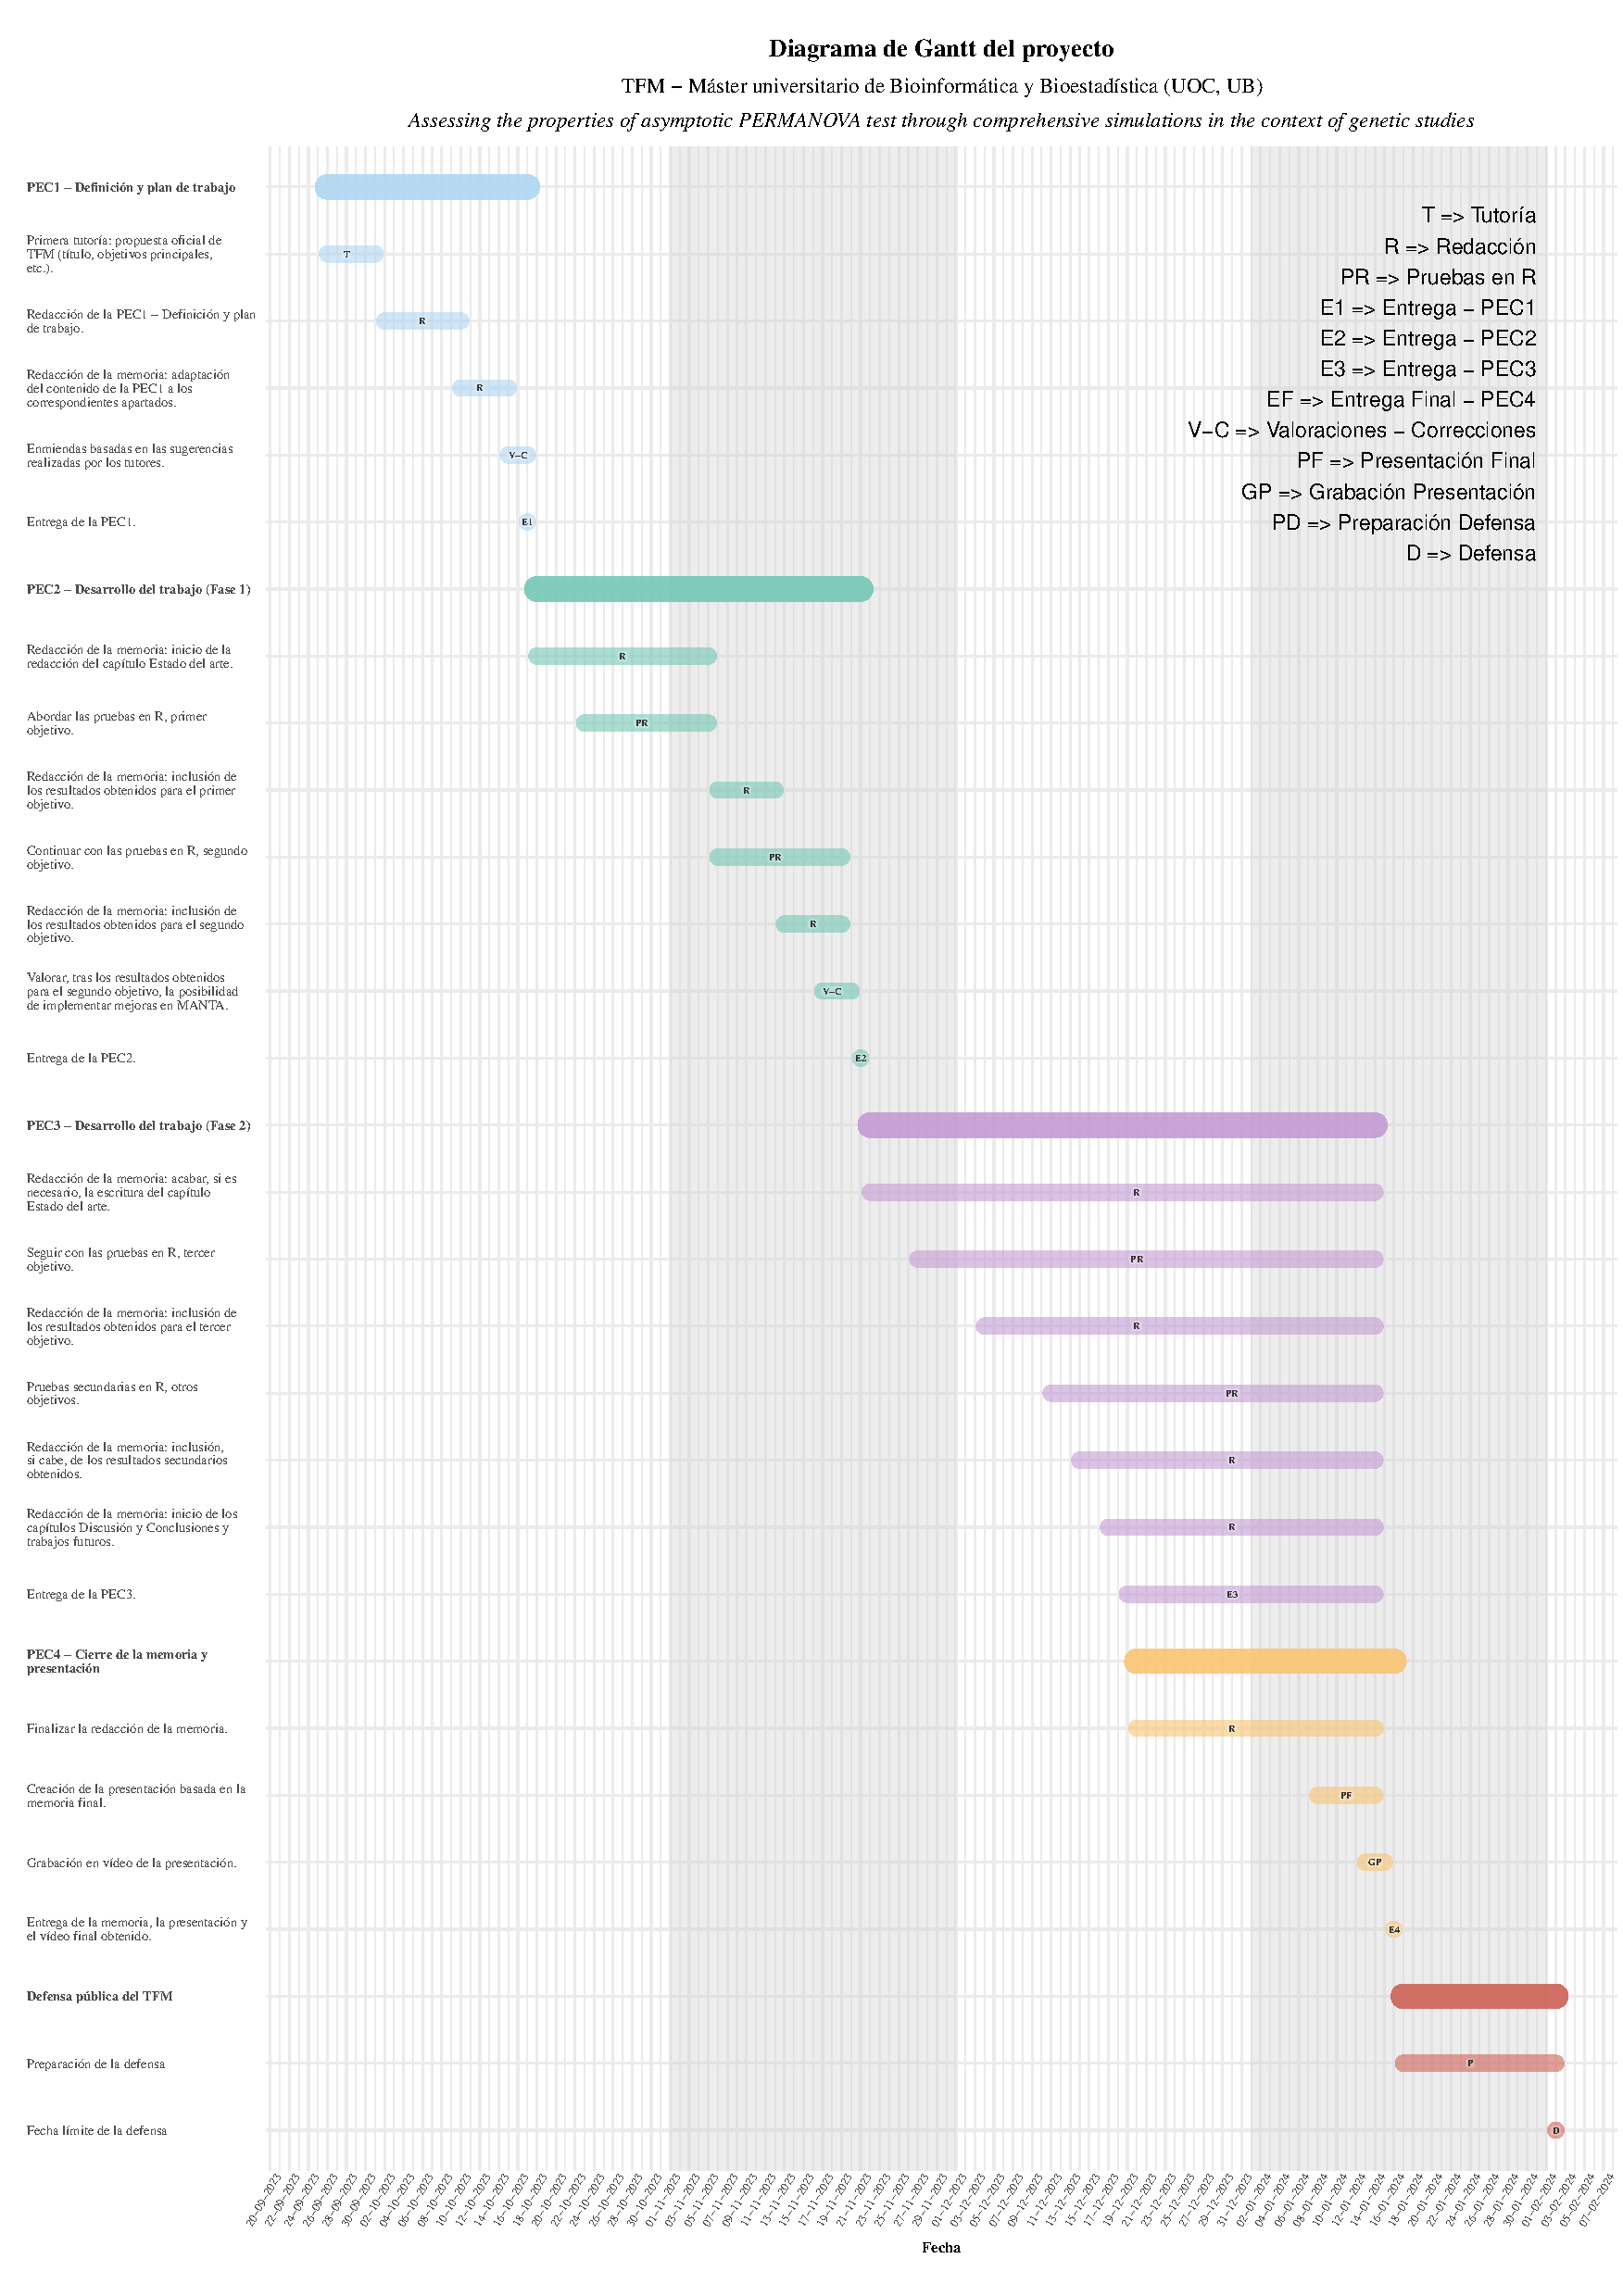
\includegraphics[scale=.5]{TFMGantt.pdf}
    \caption{\scriptsize{Planificación ideada de las tareas necesarias para la consecución de la memoria y presentación del presente TFM.}}
    \label{fig:PEC3 - GANTT_TFM}
\end{figure}


\newpage\null\thispagestyle{empty} % Página en blanco para separar la Memoria de las PEC

\Huge
\vfill

\textbf{Memoria}
\normalsize

\newpage



%%%%%%%%%%%%%%%%%%%
% Memoria del TFM %
%%%%%%%%%%%%%%%%%%%

%%%%%%%%%%%%%%%%%%%%%%%%%%%%%%%%%%%%%%%%%%
% Primera parte: Introducción  <--> PEC1 %
%%%%%%%%%%%%%%%%%%%%%%%%%%%%%%%%%%%%%%%%%%


\chapter{Introducción}
\label{chap:Introducción}


\section{Contexto y justificación del trabajo}
\label{sec:Contexto y justificación del trabajo}

% Contextualizad el TFM, explicad a qué ámbito pertenece, y justificad su interés: explicad por qué el trabajo que habéis elegido es interesante.


% Propuesta de TFM (D. Garrido y M. Calvo):
%
%  Título: Assessing the properties of asymptotic PERMANOVA test through comprehensive
%          simulations in the context of genetic studies
%
%  Objetivos principales:
%
%    - Estudio de potencia con distintas transformaciones (sqrt, log, datos composicionales, etc.)
%    - Estudio de la pérdida de potencia con respecto a MANOVA con P-valores pequeños
%    - Evaluación comparativa del método de Davies y el propuesto en Yang J. et al.
%      (implementación en C/C++)
%
%  Comentarios PEC1 (D. Garrido y M. Calvo):
%
%    - Acordarse que en todo caso trabajamos con la versión asintótica de PERMANOVA,
%                no con PERMANOVA!!! 
%
%    - Descripción más detallada:
%
%      a) GWAS y QTL mapping
%      b) Cómo en estos análisis se usan sobre todo métodos univariantes
%      c) Ventajas de las aproximaciones multivariantes
%      d) Limitaciones (parametricas, running time)
%      e) Cómo PERMANOVA puede ser una buena alternativa, pero necesita permutaciones,
%         razón por la que hemos desarrollado MANTA (= asymptotic PERMANOVA)
%      f) Aquí entra tu TFM: estudiar las propiedades de MANTA en algunos escenarios,
%         comparar transformaciones, estudiar pérdida de potencia vs MANOVA y otros métodos
%         (reportada en este artículo: https://www.nature.com/articles/s41588-022-01154-4), 
%         implementaciones (e.g. Farebrother -current- vs Saddlepoint), etc.
%         Nosotros ya hicimos benchmark Davies vs Farebrother vs Imhof vs Liu, aunque se puede ampliar,
%         el objetivo fundamental es comparar Farebrother con Saddlepoint.


El tema escogido para la realización del TFM se enmarca en el análisis de datos ómicos mediante el uso de la \textit{\gls{estadística multivariante}}, principalmente la versión asintótica de \textit{\gls{PERMANOVA}}, aplicada al estudio de asociaciones entre los polimorfismos de un solo nucleótido (\textit{\gls{SNPs}}) del genoma completo (estudios tipo \textit{\gls{GWAS}}) y algunos rasgos característicos, como son las principales enfermedades humanas, así como en la detección de \textit{\gls{sQTLs}} utilizando datos \textit{\gls{RNA-seq}}.

%      a) GWAS y QTL mapping
%      b) Cómo en estos análisis se usan sobre todo métodos univariantes

Originalmente, las investigaciones basadas en \textit{GWAS}, ya sea integrando \textit{sQTLs} o no, se han realizado con la finalidad de comprobar la asociación entre los \textit{SNPs} con diferentes variantes genéticas mediante el estudio de un único rasgo (única variable o \textit{\gls{trait}}), con lo que los análisis estadísticos correspondientes llevados a cabo suelen utilizar, lógicamente, los principales métodos univariantes disponibles (sumario estadístico basado en tablas de distribución de frecuencias, estadísticos de centralización o dispersión, etc.).

De este modo, este tipo de estudios, al centrarse en un solo \textit{trait} de todos los disponibles en el gran volumen de datos sobre fenotipos utilizable, no permiten tratar la posible relación causa-efecto subyacente, obteniendo un análisis meramente descriptivo. \\

%      c) Ventajas de las aproximaciones multivariantes
%      d) Limitaciones (parametricas, running time)
%      e) Cómo PERMANOVA puede ser una buena alternativa, pero necesita permutaciones,
%         razón por la que hemos desarrollado MANTA (= asymptotic PERMANOVA)

Alternativamente, gracias a la gran cantidad de datos disponibles últimamente con perfiles genómicos complejos (alta diversidad de rasgos moleculares), la necesidad de encontrar correlaciones entre las diferentes variables analizables y los rasgos de interés, ha resultado en un crecimiento en la utilización de métodos multivariantes para su análisis estadístico.

Las principales ventajas con respecto al enfoque univariante clásico, para poder determinar la posible estructura de correlaciones subyacente en los datos, pueden enumerarse como sigue:

{\small
\begin{itemize}
    \item Mayor \textit{\gls{potencia estadística}} (\( \mathbb P \)) para detectar asociaciones genéticas.
    \item Ofrece ventajas en el estudio de la \hspace{-.25em}\textit{\gls{pleiotropía}} (cuando el gen o alelo considerado es responsable de efectos fenotípicos o caracteres distintos y, a priori, no relacionados).
    \item Resulta de utilidad incluso cuando solo un pequeño grupo de los rasgos se ve afectado por el genotipo de interés.
    \item Permite el análisis a través de múltiples capas fenotípicas en bloque, dando luz sobre los mecanismos moleculares activados por las variantes genéticas consideradas.
    \item Posibilita la caracterización de los efectos genéticos sobre un mismo rasgo cuando este es medido en diferentes condiciones ambientales o entornos.
    \item Requiere de menos pruebas individuales, lo que disminuye las de carácter múltiple.
\end{itemize}}

Contrariamente, del uso de los métodos más habitualmente utilizados para estudiar estas asociaciones genéticas multirasgo emergen diversos inconvenientes, entre los cuales destacan:

{\small
\begin{itemize}
    \item Los métodos que modelan el genotipo como variable dependiente comprobando a su vez la asociación con una suma ponderada de fenotipos (\textit{MV-PLINK} (\cite{ferreira_multivariate_2009}) o análisis de correlación canónica, y \textit{\gls{MultiPhen}} \cite{coin_multiphen_2020} que utiliza la regresión ordinal) adolecen de la posibilidad de evaluar diseños complejos que presentan mutiples interacciones entre el genotipo y otras covariables.
    \item Tanto el análisis multivariante de la varianza (\textit{\gls{MANOVA}}), como el de los modelos multivariantes lineales mixtos (\textit{\gls{mvLMMs}}) \cite{zhou_efficient_2014}, resultan ser más tolerantes a estos diseños complejos al tratar los fenotipos como variables dependientes, introduciendo de froma natural el posible parentesco genético entre los individuos analizados. Esta ventaja se torna inconveniente para grandes conjuntos de datos, sobre todo para el método \textit{mvLMMs}, cuya continua mejora en su implementación computacional sigue requiriendo de tiempos excesivamente altos. 
    \item La pluralidad de los métodos de regresión multivariante presuponen una normalidad en la distribución de los errores del modelo que puede no llegar a cumplirse. Todo y que pueden aplicarse transformaciones individuales a cada rasgo estudiado, no puede garantizarse la normalidad multivariante, lo que resulta en una reducción de la potencia estadística en comparación con el modelo aplicado a los rasgos no transformados.
    \item Hasta el momento, las diversas implementaciones de \textit{métodos bayesianos} para el estudio de asociaciones multirasgo no han sido satisfactorias, requiriendo siempre un tiempo elevado de cálculo debido al coste computacional que implican.
    \item Para los métodos \textit{\gls{MTAR}} \cite{luo_multi-trait_2020} o \textit{\gls{MOSTest}} \cite{noauthor_precimedmostest_2023} \cite{van_der_meer_understanding_2020} existe la necesidad de garantizar la normalidad multivariante asintótica cuando se utilizan los sumarios estadísticos univariantes, lo que no es trivial, sumado a que evitar la aparición de sesgos en la estimación de correlaciones de rasgos a partir de esta clase de estadísticos no es sencillo (afectaciones de heredabilidad de los rasgos, patrones de desequilibrio de ligamiento, etc.).
\end{itemize}}

Con todo lo anterior, resulta evidente la necesidad de disponer de un método no paramétrico adecuado tanto para los estudios basados en (\textit{GWAS}) como en \textit{sQTLs}. El modelo de \textit{PERMANOVA} (\cite{anderson_new_2001}) amplía el modelo lineal factorial univariante a múltiples dimensiones sin requerir una distribución de probabilidad conocida de las variables dependientes, introduciendo un enfoque basado en la distancia, poniendo a prueba la hipótesis de ausencia de efectos mediante un procedimiento de permutación basado en un estadístico \textit{\gls{pseudo-F}}, en el que las sumas de cuadrados del \textit{ANOVA} se sustituyen por sumas de interdistancias entre observaciones.\\
Pese a ser exitoso en muchos estudios, dando buenos resultados en un tiempo de cálculo reducido para diseños fijos unidireccionales, resulta inviable en los estudios actuales, donde el mayor tamaño y complejidad de los conjuntos de datos requiere una precisión para el cálculo del valor p que este procedimiento permutacional no puede alcanzar en las condiciones requeridas.

El punto de partida del presente trabajo radica en los diversos estudios realizados con el fin de superar esta limitación. En concreto: sendos artículos de Garrido-Martín, D. \textit{et al.} (\cite{garrido-martin_fast_2022} y \cite{garrido-martin_identification_2021}), y el trabajo de Monlong, J. \textit{et al.} \cite{monlong_identification_2014}. Donde, gracias al programa \textit{\gls{MANTA}} (\cite{garrido-martin_manta_2023}, desarrollado principalmente en \hspace{-.2em}\Rlogo\hspace{+.1em}), se estudia mediante diversas simulaciones (\cite{garrido-martin_manta-sim_2022}) de diseños complejos la distribución asintótica de la estadística de pruebas \textit{PERMANOVA} en el caso de la distancia euclídea (\textit{\gls{valores p}} de carácter no paramétrico y asintótico para modelos lineales multivariados), obteniendo resultados igualmente válidos tras cualquier transformación de los datos que preserve la independencia de las observaciones.

%      f) Aquí entra tu TFM: estudiar las propiedades de MANTA en algunos escenarios,
%         comparar transformaciones, estudiar pérdida de potencia vs MANOVA y otros métodos
%         (reportada en este artículo: https://www.nature.com/articles/s41588-022-01154-4), 
%         implementaciones (e.g. Farebrother -current- vs Saddlepoint), etc.
%         Nosotros ya hicimos benchmark Davies vs Farebrother vs Imhof vs Liu, aunque se puede ampliar,
%         el objetivo fundamental es comparar Farebrother con Saddlepoint.

\

La finalidad principal será ahondar en estos estudios, yendo más allá en al menos los siguientes aspectos:


\begin{itemize}
    \item Estudiar las propiedades de \textit{MANTA} en algunos escenarios, determinando cómo los diferentes tipos de transformaciones de datos afectan a los resultados obtenidos, y dilucidar si existe algún protocolo privilegiado en las simulaciones implementadas.
    \item Estudiar la pérdida de potencia de la versión asintótica de \textit{PERMANOVA} con respecto a \textit{MANOVA} y otros métodos, profundizando en la afectación de la variación del nivel de significación considerado sobre la potencia de cada uno.
    \item Comparar los resultados obtenidos con respecto al cálculo de la distribución de las formas cuadráticas entre el método Farebrother (implementado para la versión asintótica de \textit{PERMANOVA} con \textit{MANTA}) y el de Saddlepoint.
    \item Extender el punto anterior, ampliando la comparativa Farebrother vs. Saddlepoint a otros métodos: métodos exactos como el de Davies, R. B. (\cite{davies_numerical_1973}, \cite{davies_algorithm_1980}), o aproximaciones numéricas como la de Liu–Tang–Zhang (\cite{qi_genetic_2022}), el método de Imhof, etc.
    \item Partiendo del caso de estudio anterior, y secundariamente, se llevaría a cabo la implementación del método más óptimo en el paquete \textit{MANTA} ya existente, en caso de que este exista.
\end{itemize}


\section{Objetivos del trabajo}
\label{sec:Objetivos del trabajo}

% Explicad a grandes rasgos en qué consistirá el TFM. Este punto no debe confundirse con una introducción, sino que también debe explicar brevemente como planeáis que sea el trabajo.


%  Comentarios PEC1 (D. Garrido y M. Calvo):
%
%    - En este contexto yo no añadiría los objetivos como tal, describe un poco si quieres pero
%      ponlos en el apartado correspondiente
%    - Quizás puedes definir un objetivo general, que sea estudiar las propiedades de MANTA en
%      distintos contextos de simulación [...] y mejorar la implementación actual y luego añadir
%      los objetivos (que ahora llamas principales) como específicos. O alternativamente desarrollar
%      un par de objetivos específicos por cada uno de los principales.


De los diferentes puntos detallados en el apartado anterior, se extrae que el presente trabajo deberá permitirnos profundizar en aspectos concretos de los estudios ya referenciados (\cite{garrido-martin_fast_2022}, \cite{garrido-martin_identification_2021}), \cite{monlong_identification_2014}), con el objetivo último de determinar la validez de la versión asintótica del método \textit{PERMANOVA} (implementado en el paquete \textit{MANTA}) con respecto a otros métodos similares bajo un mismo conjunto de simulaciones computacionales complejas basadas en datos de escenarios reales.

\newpage

% Explicad claramente tanto los objetivos generales como los específicos:
% Objetivos generales: Deben ser pocos (quizás un par o máximo tres) y suficientemente amplios para cubrir todo el alcance del proyecto. Deben estar redactados de forma concreta y evaluable.
% Objetivos específicos: desglosad cada objetivo general en otros más concretos (no confundir con tareas). Se deben redactar con un verbo en infinitivo de significado medible (no puede ser por ejemplo “saber” porque no se puede medir  o evidenciar su cumplimiento).

Según las bases generales establecidas, y para una consecución satisfactoria del estudio propuesto, se han considerado los siguientes objetivos principales:

{\small
\begin{itemize}
    \item Estudiar las propiedades de \textit{MANTA} en algunos escenarios, determinando cómo los diferentes tipos de transformaciones de datos afectan a los resultados obtenidos, y dilucidar si existe algún protocolo privilegiado en las simulaciones implementadas.
    \item Estudiar la pérdida de potencia de la versión asintótica de \textit{PERMANOVA} con respecto a \textit{MANOVA} y otros métodos, profundizando en la afectación de la variación del nivel de significación considerado sobre la potencia de cada uno.
    \item Comparar los resultados obtenidos con respecto al cálculo de la distribución de las formas cuadráticas entre el método Farebrother (implementado para la versión asintótica de \textit{PERMANOVA} con \textit{MANTA}) y el de Saddlepoint.
\end{itemize}}

Como extensión de los mismos, resulta también conveniente establecer otros objetivos secundarios:

{\small
\begin{itemize}
    \item Extender el tercer objetivo principal, ampliando la comparativa Farebrother vs. Saddlepoint a otros métodos: métodos exactos como el de Davies, R. B. (\cite{davies_numerical_1973}, \cite{davies_algorithm_1980}), o aproximaciones numéricas como la de Liu–Tang–Zhang (\cite{qi_genetic_2022}), el método de Imhof, etc.
    \item Partiendo del caso de estudio anterior, se llevaría a cabo la implementación del método más óptimo en el paquete \textit{MANTA} ya existente, en caso de que los resultados obtenidos indiquen que alguno de ellos resulta ser más eficiente tanto computacional como estadísticamente hablando.
\end{itemize}}


% \section{Impacto en sostenibilidad, ético-social y de diversidad}
% \label{sec:Impacto en sostenibilidad, ético-social y de diversidad}
% 
% Esta sección tendría que identificar los impactos positivos y/o negativos del trabajo final en las tres dimensiones de la competencia transversal UOC “Compromiso ético y global”.
% 
% La Guía transversal sobre la Competencia Ética y Global os ayudará a redactar estos apartados.


\section{Enfoque y método seguido}
\label{sec:Enfoque y método seguido}

% Mención de cuáles son las posibles estrategias para llevar a cabo el trabajo y cuál es la estrategia elegida (desarrollar un producto nuevo, adaptar un producto existente...). Hay que incluir una valoración de por qué esta es la estrategia más apropiada para conseguir los objetivos.


% Indicad cuáles son las posibles estrategias para llevar a cabo el trabajo e indicar cuál es la elegida. Valorad por qué ésta es la más apropiada para lograr los objetivos.


%  Comentarios PEC1 (D. Garrido y M. Calvo):
%
%    - Desarrolla una lista de tareas y método a seguir, así como una planificación orientativa (Gannt).
%      Entiendo que serán preliminares, pero en cualquier caso estaría bien que te plantearas las
%      distintas tareas, así como que hicieras una pequeña evaluación de riesgos.

En cuanto al tiempo de dedicación, se ha enfocado el trabajo adaptando las tareas ideadas para la consecución de los diferentes objetivos marcados a las pautas establecidas por las diferentes entregas programadas por la UOC (\textit{Pruebas de Evaluación Continua} o \textit{PEC}), pudiendo destacar los siguientes grandes bloques de trabajo y la estimación del peso que estos han tenido en el tiempo dedicado al proyecto:

 % - Primera entrega: PEC1 - Definición y plan de trabajo
 %   * Primera tutoría: propuesta oficial de TFM (título, objetivos principales, etc.).
 %   * Redacción de la PEC1 - Definición y plan de trabajo.
 %   * Redacción de la memoria: adaptación del contenido de la PEC1 a los correspondientes apartados.
 %   * Enmiendas basadas en las sugerencias realizadas por los tutores.
 %   * Entrega de la PEC1.
 % 
 % - Segunda entrega: PEC2 - Desarrollo del trabajo - Fase 1
 %   * Redacción de la memoria: inicio de la redacción del capítulo Estado del arte.
 %   * Abordar las pruebas en R, primer objetivo: estudiar las propiedades de MANTA en algunos escenarios
 %   comparando diferentes transformaciones de los datos.
 %   * Redacción de la memoria: inclusión de los resultados obtenidos para el primer objetivo.
 %   * Continuar con las pruebas en R, segundo objetivo: estudiar la pérdida de potencia de la versión asintótica
 %   de PERMANOVA con respecto a MANOVA y otros métodos.
 %   * Redacción de la memoria: inclusión de los resultados obtenidos para el segundo objetivo.
 %   * Valorar, tras los resultados obtenidos para el segundo objetivo, la posibilidad de implementar mejoras en MANTA.
 %   * Entrega de la PEC2.
 % 
 % - Tercera entrega: PEC3 - Desarrollo del trabajo - Fase 2
 %   * Redacción de la memoria: acabar, si es necesario, la escritura del capítulo Estado del arte.
 %   * Seguir con las pruebas en R, tercer objetivo: comparar los resultados obtenidos con respecto al cálculo de la
 %   distribución de las formas cuadráticas entre el método Farebrother (implementado para la versión asintótica de
 %   PERMANOVA con MANTA y el de Saddlepoint.
 %   * Redacción de la memoria: inclusión de los resultados obtenidos para el tercer objetivo.
 %   * Pruebas secundarias en R, otros objetivos: extender el tercer objetivo, ampliando la comparativa Farebrother
 %   vs. Saddlepoint a otros métodos (Davies, Imhof, Liu, etc.).
 %   * Redacción de la memoria: inclusión, si cabe, de los resultados secundarios obtenidos.
 %   * Redacción de la memoria: inicio de los capítulos Discusión y Conclusiones y trabajos futuros.
 %   * Entrega de la PEC3.
 % 
 % - Cuarta entrega: PEC4 - Cierre de la memoria y de la presentación
 %   * Finalizar la redacción de la memoria: adaptación del contenido generado en las diferentes PEC  a los cor-
 %   respondientes apartados, finalizando las secciones anexas (Bibliografía, Glosario, etc.).
 %   * Creación, bajo los criterios establecidos, de la presentación basada en la memoria final.
 %   * Grabación en vídeo de la presentación.
 %   * Entrega de la memoria, la presentación y el vídeo final obtenido (sendas copias en el REC y la aplicación Present@).

\footnotesize
\begin{itemize}
    \item \textbf{Primera fase o entrega (PEC1):} definición y plan de trabajo.\\
    \(\Rightarrow\) \textit{Dedicación estimada:} 3 \% del tiempo total final destinado al trabajo.
    \item \textbf{Segunda fase o entrega (PEC2):} primera fase del desarrollo del trabajo.\\
    \(\Rightarrow\) \textit{Dedicación estimada:} 35 \% del tiempo total final destinado al trabajo.
    \item \textbf{Tercera fase o entrega (PEC3):} segunda fase del desarrollo del trabajo.\\
    \(\Rightarrow\) \textit{Dedicación estimada:} 45 \% del tiempo total final destinado al trabajo.
    \item \textbf{Cuarta fase o entrega (PEC4):} cierre de la memoria y preparación de los documentos pertinentes.\\
    \(\Rightarrow\) \textit{Dedicación estimada:} 15 \% del tiempo total final destinado al trabajo.
    \item \textbf{Defensa pública:} Preparación de la defensa pública en base a la memoria final del proyecto.\\
    \(\Rightarrow\) \textit{Dedicación estimada:} 2 \% del tiempo total final destinado al trabajo.
\end{itemize}
\normalsize

Se puede encontrar una planificación más detallada en las secciones \textit{\hyperref[sec:Planificación del trabajo]{Planificación del trabajo}} e \textit{\hyperref[sec:Hitos]{Hitos}}, y una recopilación de los contratiempos encontrados y sus correspondientes enmiendas en la sección \textit{\hyperref[sec:Desviaciones en la planificación y acciones de mitigación]{Desviaciones en la planificación y acciones de mitigación}}.

\newpage
Con respecto al enfoque práctico, y a la metodología específica de trabajo seguida, caben destacar los siguientes aspectos:

\footnotesize
\begin{itemize}
        \item Estudio inicial detallado de los principales artículos de referencia: \cite{garrido-martin_fast_2022}, \cite{garrido-martin_identification_2021}), \cite{monlong_identification_2014}.
    \item Estudio en profundidad del método \textit{PERMANOVA} implementado en el paquete \textit{MANTA} (\cite{garrido-martin_manta_2023}), haciendo hincapié en la comprensión de la estructura del algoritmo implementado, y en la labor de cada una de las funciones implicadas.
    \item Estudio en profundidad de las diferentes simulaciones utilizadas en \cite{garrido-martin_fast_2022} (\cite{garrido-martin_manta-sim_2022}), con la finalidad de comprender el propósito de cada una de ellas en dicho trabajo e identificar el escenario en el cual el presente trabajo puede aportar más información.
    \item Implementación en \hspace{-.2em}\Rlogo\hspace{+.1em} del algoritmo necesario para realizar las simulaciones requeridas en el estudio de cada uno de los objetivos especificados, partiendo de la estructura original presente en \cite{garrido-martin_manta-sim_2022}, pero adaptando pertinentemente los escenarios de simulación adecuados.
    \item Pruebas del código implementado con diferentes finalidades: estudio de los resultados obtenidos bajo diversas combinaciones de las variables implicadas, salvaguardado oportuno de los datos producidos para su posterior análisis y utilización en la memoria, determinación de la visualización gráfica más apropiada en cada caso 
    \item Subsanado continuo de los errores obtenidos en la ejecución del código implementado.
    \item Evaluación y análisis con respecto al propósito original del proyecto de los resultados finales logrados.
\end{itemize}
\normalsize


% \begin{landscape}
\section{Planificación del trabajo}
\label{sec:Planificación del trabajo}

% Descripción de los recursos necesarios para hacer el trabajo, las tareas a realizar y una planificación temporal de cada tarea mediante un diagrama de Gantt o similar. Esta planificación tendría que marcar cuáles son los hitos parciales de cada una de las PEC.

% Desglosad las tareas que vais a hacer para conseguir vuestros objetivos y proponed una planificación temporal. 
% Tareas: Enumerad las diversas tareas en que se han desglosado los objetivos y la duración que se asigna a cada una. Tiene que haber una coherencia numérica entre objetivos generales, objetivos específicos y tareas.
% Calendario: Es recomendable usar un programa específico de planificación para generar un diagrama de Gantt que se pueda insertar en el documento.
% Hitos: Los hitos marcan los estados intermedios del proyecto y permiten avanzar en sucesivas etapas de resultados prácticos, por ejemplo, tomando decisiones relevantes. Es imprescindible que seáis estrictos en el cumplimiento de las fechas que os marquéis. Será importante que os baséis en el Plan Docente y concretamente en las fechas clave que se indican allá para elaborar vuestra planificación.
% Análisis de riesgos: Enumerad y comentad qué factores pueden repercutir negativamente en el seguimiento del plan de trabajo y en la consecución del proyecto. Hay dos factores que tienen influencia en cualquier proyecto: el alcance del proyecto  y el tiempo del que disponéis para realizarlo. Hay otros riesgos asociados a las características específicas de cada TFM y al método de investigación y/o de desarrollo que se utiliza. Igual que los objetivos, deben ser concretos. 

Tras analizar los objetivos marcados al inicio del proyecto, y considerar el ritmo de avance en la obtención de los resultados previstos en el plan de trabajo (\ref{fig:GANTT_TFM}), cabe destacar que se puede dar por completado el estudio del primer y segundo objetivo. Por otro lado, y pese a que se hicierón algunas pruebas preliminares, la implementación definitiva de las simulaciones necesarias para el estudio del tercer objetivo y su posterior evaluación ha tenido que ser pospuesta a futuros trabajos, ya que la fase de redacción final del trabajo no deja el tiempo suficiente para su realización sin poner en peligro la finalización del proyecto dentro de las fechas establecidas. 

En particular, tanto para el primer como para el segundo objetivo, y después de implementar diversos escenearios, algunos fallidos y otros exitosos, se han introducido ciertos cambios de criterio para establecer las simulaciones que debían ser relevantes para obtener los resultados que se buscaban en el proyecto actual. Este hecho ha aumentado el tiempo dedicado a las simulaciones en \hspace{-.2em}\Rlogo\hspace{+.1em}, en detrimento de la redacción de la memoria, conllevando la alteración final del orden de algunas tareas, e incluso la anulación de otras inicialmente previstas.

Recapitulando, se estima que la alteración y reestructuración de dicha planificación puede traducirse en que el proyecto final representará entorno al 80 \% de los objetivos del original. La planificación final de las tareas que han conformado cada bloque de trabajo específico puede encontrarse en \ref{fig:GANTT_TFM}. 

% \footnote{Esta página se muestra de forma apaisada deliberadamente, con tal de acomodar la imagen correctamente.}

\begin{figure}[!htbp]
    \centering
    % \includegraphics[width=22truecm]{GANTT_TFM.png}
    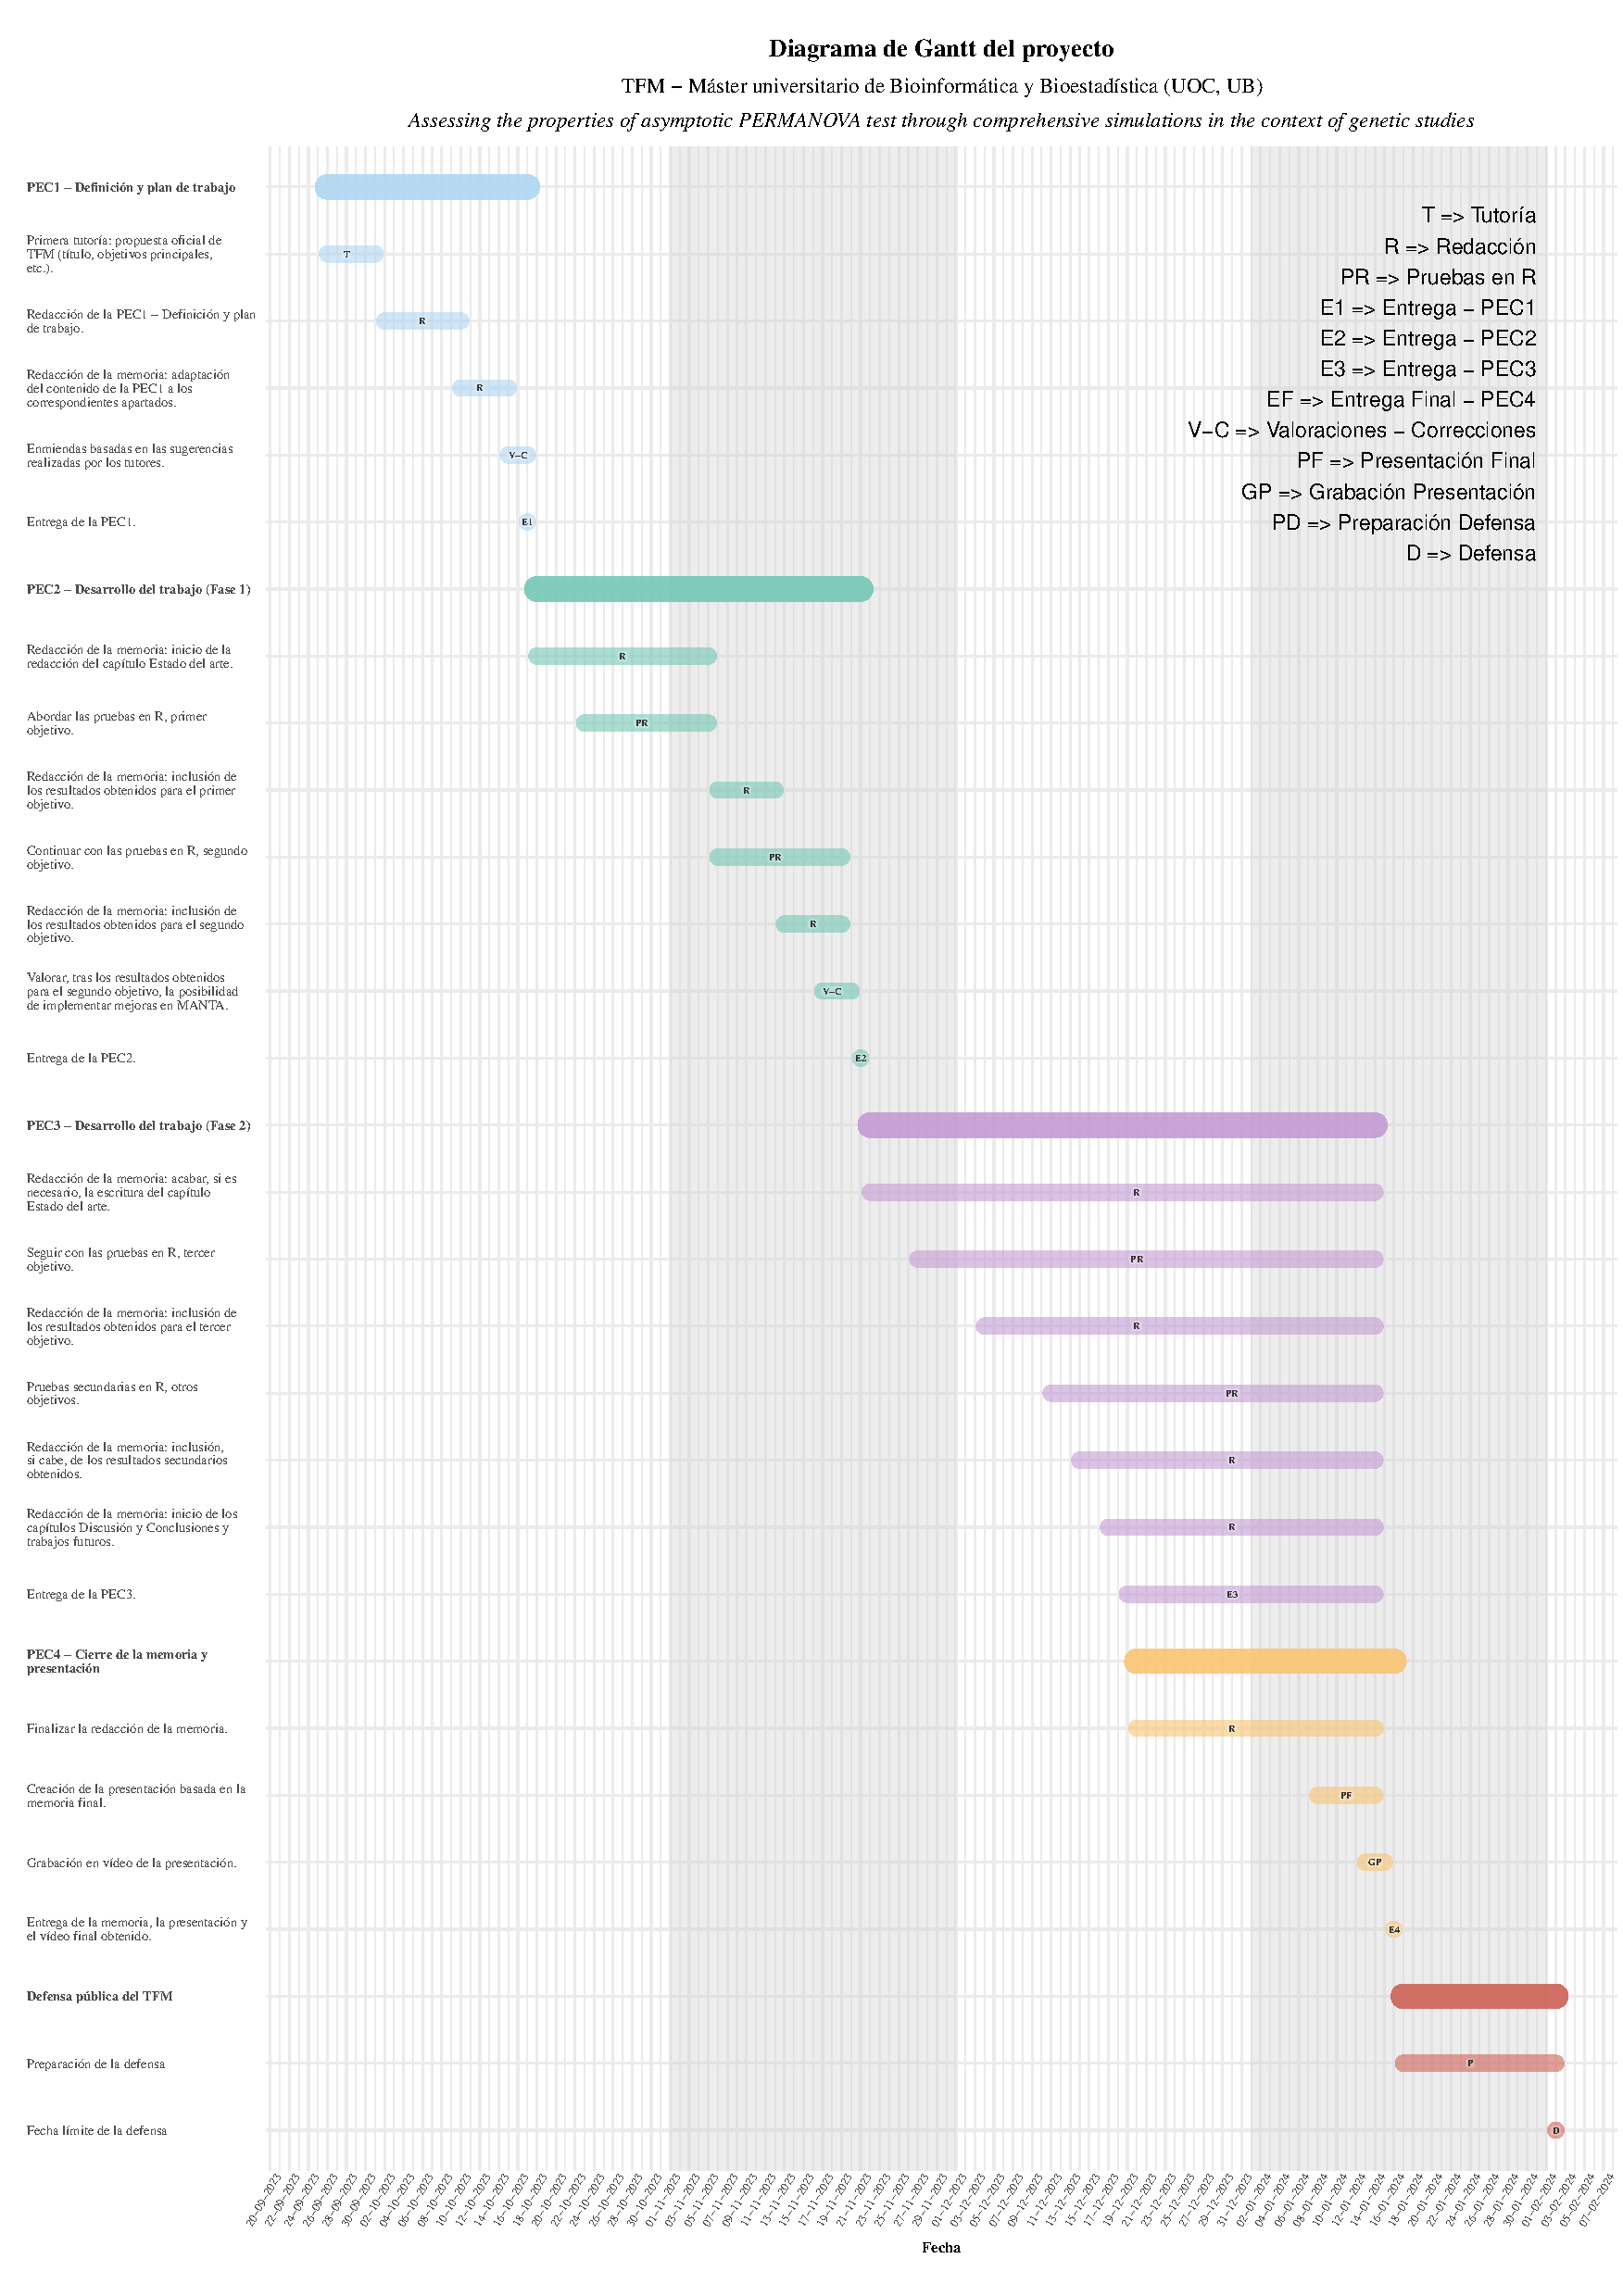
\includegraphics[scale=.5]{TFMGantt.pdf}
    \caption{\scriptsize{Planificación ideada de las tareas necesarias para la consecución de la memoria y presentación del presente TFM.}}
    \label{fig:GANTT_TFM}
\end{figure}


\newpage
% \end{landscape}


\section{Hitos}
\label{sec:Hitos}

A continuación se muestran las distintas fases del proyecto según su compleción, indicando los posibles retrasos o problemas inesperados o no que, al surgir, pueden haber puesto en riesgo la consecución de las tareas previstas, y los objetivos establecidos:

% Crear una lista con checkbox:
% Dentro del "todolist": \item, \item[\done] o \item[\wontfix] (Antiguos: \item[\cmark], \item[\xmark])

\begin{todolist}
  \item[\done] \textbf{Primera entrega:} \textit{PEC1 - Definición y plan de trabajo}
  \begin{todolist}
  \item[\done] Primera tutoría: propuesta oficial de TFM (título, objetivos principales, etc.).
  \item[\done] Redacción de la \textit{PEC1 - Definición y plan de trabajo}.
  \item[\done] Redacción de la memoria: adaptación del contenido de la \textit{PEC1} a los correspondientes apartados.
  \item[\done] Enmiendas basadas en las sugerencias realizadas por los tutores.
  \item[\done] Entrega de la \textit{PEC1}.
  \end{todolist}
\end{todolist}

\begin{todolist}
  \item[\done] \textbf{Segunda entrega:} \textit{PEC2 - Desarrollo del trabajo - Fase 1}
  \begin{todolist}
  \item[\progress] Redacción de la memoria: inicio de la redacción del capítulo \textit{Estado del arte}.
  \item[\done] Abordar las pruebas en \hspace{-.2em}\Rlogo\hspace{+.1em}, primer objetivo: estudiar las propiedades de \textit{MANTA} en algunos escenarios comparando diferentes transformaciones de los datos. EL tiempo de dedicación fue ligeramente más elevado del estimado originalmente.
  \item[\progress] Redacción de la memoria: inclusión de los resultados obtenidos para el primer objetivo. Pospuesta a la parte final del proyecto, una vez acabadas las simulaciones y obtenidos los resultados.
  \item[\done] Continuar con las pruebas en \hspace{-.2em}\Rlogo\hspace{+.1em}, segundo objetivo: estudiar la pérdida de potencia de la versión asintótica de \textit{PERMANOVA} con respecto a \textit{MANOVA} y otros métodos. En este caso, el tiempo de dedicación creció más de lo esperado con respecto al estimado en un principio, ya que surgieron diversos errores en el desarrollo de las simulaciones.
  \item[\progress] Redacción de la memoria: inclusión de los resultados obtenidos para el segundo objetivo. Pospuesta a la parte final del proyecto, una vez acabadas las simulaciones y obtenidos los resultados.
  \item[\wontfix] Valorar, tras los resultados obtenidos para el segundo objetivo, la posibilidad de implementar mejoras en \textit{MANTA}. Para no poner en peligro la consecución de los plazos establecidos, se ha decidido posponer a futuros trabajos este objetivo secundario, derivado directamente del anteriormente mencionado.
  \item[\done] Entrega de la \textit{PEC2}.
  \end{todolist}
\end{todolist}

\newpage

\begin{todolist}
  \item[\done] \textbf{Tercera entrega:} \textit{PEC3 - Desarrollo del trabajo - Fase 2}
  \begin{todolist}
  \item[\progress] Redacción de la memoria: acabar, si es necesario, la escritura del capítulo \textit{Estado del arte}. Pospuesta a la parte final del proyecto, una vez acabadas las simulaciones y obtenidos los resultados.
  \item[\wontfix] Seguir con las pruebas en \hspace{-.2em}\Rlogo\hspace{+.1em}, tercer objetivo: comparar los resultados obtenidos con respecto al cálculo de la distribución de las formas cuadráticas entre el método \textit{Farebrother} (implementado para la versión asintótica de \textit{PERMANOVA} con \textit{MANTA}) y el de \textit{Saddlepoint}. Pese a haberse realizado algunas simulaciones preliminares, se ha aplazado a posteriores trabajos por falta de tiempo.
  \item[\wontfix] Redacción de la memoria: inclusión de los resultados obtenidos para el tercer objetivo. Este punto no se ha llevado a cabo por haber sido aplazado a posteriores trabajos el objetivo correspondiente.
  \item[\wontfix] Pruebas secundarias en \hspace{-.2em}\Rlogo\hspace{+.1em}, otros objetivos: extender el tercer objetivo, ampliando la comparativa \textit{Farebrother} vs. \textit{Saddlepoint} a otros métodos (\textit{Davies}, \textit{Imhof}, \textit{Liu}, etc.). Este punto no se ha llevado a cabo por haber sido aplazado a posteriores trabajos el objetivo correspondiente.
  \item[\wontfix] Redacción de la memoria: inclusión, si cabe, de los resultados secundarios obtenidos. Pospuesta a la parte final del proyecto, una vez acabadas las simulaciones y obtenidos los resultados.
  \item[\progress] Redacción de la memoria: inicio de los capítulos \textit{Discusión} y \textit{Conclusiones y trabajos futuros}. Pospuesta a la parte final del proyecto, una vez acabadas las simulaciones y obtenidos los resultados.
  \item[\done] Entrega de la \textit{PEC3}.
  \end{todolist}
\end{todolist}

\begin{todolist}
  \item[\progress] \textbf{Cuarta entrega:} \textit{PEC4 - Cierre de la memoria y de la presentación}
  \begin{todolist}
  \item[\progress] Finalizar la redacción de la memoria: adaptación del contenido generado en las diferentes \textit{PEC} a los correspondientes apartados, finalizando las secciones anexas (\textit{Bibliografía}, \textit{Glosario}, etc.).
  \item[\progress] Creación, bajo los criterios establecidos, de la presentación basada en la memoria final.
  \item[\progress] Grabación en vídeo de la presentación.
  \item Entrega de la memoria, la presentación y el vídeo final obtenido (sendas copias en el \textit{REC} y la aplicación \textit{Present@}).
  \end{todolist}
\end{todolist}

\begin{todolist}
  \item \textbf{Defensa:} \textit{Preparación para la defensa pública del TFM}
  \begin{todolist}
  \item Preparación de la defensa a la espera de la asignación definitiva de fecha.
  \item Defensa pública síncrona del TFM ante el tribunal asignado.
  \end{todolist}
\end{todolist}


\section{Desviaciones en la planificación y acciones de mitigación}
\label{sec:Desviaciones en la planificación y acciones de mitigación}

Como ya se ha avanzado en los pormenores de la sección \textit{\hyperref[sec:Hitos]{Hitos}}, han habido ciertas desviaciones en la temporización, en particular, con el tiempo necesario para completar correctamente el primer y segundo objetivo, lo que ha hecho necesario implementar las acciones de mitigación pertinentes:

\footnotesize

\begin{itemize}
    \item Cambiar el orden de prioridad, y el tiempo asignado, a las tareas relacionadas con el estudio del primer y segundo objetivo.
    \item Priorizar la obtención de resultados concretos en detrimento del estudio de escenarios, a priori, no tan relevantes.
    \item Transferir parte del tiempo previsto a la redacción en favor de la implementación correcta del codigo necesario, y de la posterior simulación de los escenarios considerados. Aplazando, así, la parte teórica a las dos últimas semanas programadas.
    \item Tras consensuarlo con los tutores, se creyó oportuno centrarse en el estudio de las dos metas principales, y posponer \textit{sine die} el estudio de la tercera y sus subsiguientes derivadas. Se valoró que el tiempo de dedicación estimado pondría en peligro la compleción del proyecto en su globalidad dentro de las fechas establecidas.
\end{itemize}

\normalsize


\section{Análisis de riesgos}
\label{sec:Análisis de riesgos}

En esta sección se añaden algunas de las contingencias que han ido surgiendo durante la realización del proyecto, indicando, a su vez, si alguna de ellas ha impedido su apropiado avance o, incluso, la no consecución de alguno de los objetivos planteados:

\footnotesize

\begin{itemize}
\item \textit{\textbf{Tiempo limitado}:} debido a que el TFM debe realizarse en un solo cuatrimestre, el tiempo disponible para desarrollar el proyecto suele ser muy ajustado. Cualquier contratiempo o retraso en la planificación, ya sea predecible o no, puede afectar gravemente a la consecución de los plazos y, eventualmente, impedir alcanzar alguno de los objetivos que se hayan planteado. Aunque se ha maximizado la dedicación al mismo con el tiempo disponible, se han identificado algunos escollos que podrían haver acabado atascando el proceso, lo cual ha sido clave para mitigar sus efectos.
\item \textit{\textbf{Planificación incorrecta}:} aunque en principio no parece que se haya realizado inicialmente una mala priorización o asignación de tiempo a las tareas pertinentes, si que nos hemos encontrado con más dificultades de las esperadas a la hora de la implementación de las simulaciones necesarias para uno de los objetivos, lo cual ha influido de manera negativa en la planificación. Como resultado, estos problemas han impedido disponer del tiempo necesario para obtener los resultados buscados en uno de los objetivos marcados.
\item \textbf{Etapa de análisis y pruebas:} como ya se ha indicado, durante esta fase han aparecido algunos contratiempos, relacionados principalmente con la dificultad en la consecución del funcionamiento deseado de algunos \textit{scripts} de código que implementan los escenarios de simulación buscados. Aunque no se produjeron problemas inesperados con el computador utilizado, la lentitud de algunos procesos de simulación, debido a la multitud de combinaciones de variables a simular, también ha hecho mella en los tiempos destinados a cada fase del trabajo.
\end{itemize}

\normalsize


\section{Breve sumario de productos obtenidos}
\label{sec:Breve sumario de productos obtenidos}

% No hay que entrar en detalle: la descripción detallada se hará en el resto de capítulos.

% En este apartado debéis concretar qué se obtendrá al final del proyecto. Tienen que ser ítems tangibles y medibles de lo que se espera obtener. Recordad que estos resultados deberán incluir los entregables que os pedimos al final del trabajo:
% Plan de trabajo.
% Memoria.
% Producto, si es que hay un producto resultado que no se incluye en la memoria, por ejemplo un artículo, un software desarrollado, etc.
% Presentación virtual.

\footnotesize

\begin{itemize}
    \item \textbf{Plan de trabajo:} documento donde se incluye una distribución de tareas según los objetivos determinados, puntos clave y tiempos necesarios (disponible en la sección \textit{\hyperref[sec:Planificación del trabajo]{Planificación del trabajo}}). Este ha ido sufriendo cambios a lo largo del proyecto (especificados en la sección \textit{\hyperref[sec:Desviaciones y acciones de mitigación]{Desviaciones y acciones de mitigación}}), debido principalmente a la alteración en el tiempo dedicado a las simulaciones necesarias, en detrimento de la realización de uno de los objetivos iniciales, y de la redacción de la memoria.
    \item \textbf{Memoria:} producto derivado de todas las entregas parciales o \textit{PEC} (basado en la estructura recomendada por la UOC), donde se detallará el contexto científico, los resultados obtenidos según el procedimiento seguido y, finalmente, las conclusiones extraídas tras su interpretación. Consta de los capítulos principales: \textit{\hyperref[chap:Introducción]{Introducción}}, \textit{\hyperref[chap:Estado del arte]{Estado del arte}}, \textit{\hyperref[chap:Resultados]{Resultados}}, \textit{\hyperref[chap:Discusión]{Discusión}} y \textit{\hyperref[chap:Conclusiones y trabajos futuros]{Conclusiones y trabajos futuros}}.
    \item \textbf{Producto:} Todos los archivos, producto de la realización de este TFM, pueden encontrarse en el repositorio de \texti{GitHub} \cite{aitor_invernon_de_campos_codigo_2024}. Como se aprecia en el resumen de los lenguajes más usados, los diferentes \textit{scripts} se han realizado principalmente en \hspace{-.2em}\Rlogo\hspace{+.1em} y en \LaTeX. Mientras que los del primer tipo implementan tanto las funciones necesarias, como las diversas simulaciones de los escenarios considerados en cada caso a estudio, los segundos han sido necesarios para producir la memoria final del presenta trabajo final de máster.
    \item \textbf{Presentación virtual del TFM:} exposición oral y visual basada en la memoria producida. En ella se resaltan los aspectos más importantes del trabajo realizado, presentando las distintas fases del proyecto de forma resumida.
    \item \textbf{Autoevaluación del proyecto:} documento que, una vez finalizado el proyecto, debe redactarse para plasmar una evaluación crítica del trabajo realizado, determinando el grado de alcance de los objetivos, y valorando los aspectos potencialmente mejorables.
\end{itemize}

\normalsize


\section{Comentarios de los directores del TFM}
\label{sec:Comentarios de los directores del TFM}

Durante todo el proceso se ha ido manteniendo un contacto periódico con los directores del proyecto con el fin de encauzar el trabajo iniciado, corregir algunos errores, y recibir recomendaciones tanto teóricas como prácticas. Esto ha permitido: clarificar diversos aspectos del proyecto, determinar más claramente algunos enfoques del mismo, redefinir las prioridades a la hora de obtener unos resultados en detrimento de otros, y a reestructurar debidamente el esquema temporal del proyecto.


\section{Descripción de otros capítulos}
\label{sec:Descripción de otros capítulos}

En esta sección se realizará, en caso de ser necesario, una escueta descripción de los diversos capítulos de la memoria.

% Breve explicación de los contenidos de cada capítulo y su relación con el proyecto global.


%  ========================================>    GLOSARIO DE LA PRIMERA PARTE HECHO A DÍA 9/5/23    <==========================================  %
%  ========================================> PRIMERA PARTE CORREGIDA ORTOGRÁFICAMENTE A DÍA 9/5/23 <==========================================  %


%%%%%%%%%%%%%%%%%%%%%%%%%%%%%%%%%%%%%%%%%%%%%%%%%%%%%%%%%%%%%%%%%%%
% Segunda parte: Estado del arte + Primeros resultados  <--> PEC2 %
%%%%%%%%%%%%%%%%%%%%%%%%%%%%%%%%%%%%%%%%%%%%%%%%%%%%%%%%%%%%%%%%%%%


\chapter{Estado del arte}
\label{chap:Estado del arte}

% Estado del arte del tema en cuestión.
% Tendría que acabar mostrando por qué el trabajo es importante y que aporta algo, y con las hipótesis del trabajo.
%
%
% En estos apartados, hay que describir:
% \begin{itemize}
%     \item Los aspectos más relevante del diseño y desarrollo del trabajo.
%     \item La metodología elegida para hacer este desarrollo, describiendo las alternativas posibles, las decisiones tomadas, y los criterios utilizados para tomar estas decisiones.
%     \item Los productos obtenidos.
% \end{itemize}

\section{Contexto biotecnológico}
\label{sec:Contexto biotecnológico}

Aunque el presente trabajo se basa esencialmente en un estudio computacional comparativo entre dos métodos estadísticos multivariantes específicos, bajo la simulación de ciertos escenarios totalmente controlados, estos pueden desempeñar un papel importante en diversos campos de investigación. En este aspecto, cabe destacar su aplicabilidad en estudios biológicos, en concreto, en el campo de la genética avanzada.

Esta disciplina ha evolucionado enormemente en las últimas décadas gracias al desarrollo de nuevas tecnologías, permitiendo identificar variantes genéticas asociadas a una amplia variedad de fenotipos y rasgos. La secuenciación de nucleótidos que conforman la molécula de \textit{ADN} permite el análisis detallado de su estructura, convirtiéndose en la herramienta idonea para identificar variantes en el material genético.

En los años 70, la \textit{secuenciación Sanger} revolucionó la investigación originando la era genómica, la cual se ha asentado gracias a la evolución que ha sufrido este campo en los últimos años debido al desarrollo de las nuevas plataformas de secuenciación de alto rendimiento (\textit{Next-Generation Sequencing} o \textit{NGS}). Estas nuevas técnicas son capaces de generar paralelamente, y de forma masiva, millones de fragmentos de \textit{ADN} en un único proceso de secuenciación, consiguiendo así el análisis de grandes cantidades de información genética en una escala inimaginable en los orígenes de esta disciplina \cite{behjati_what_2013,noauthor_next-generation_nodate}.

Recientemente, cada vez más investigaciones han empezado a decantarse por un tipo específico de secuenciación masiva: la \textit{secuenciación de ARN} o \textit{RNA-seq}. Dicha estrategia de análisis utiliza técnicas \textit{NGS} para revelar la presencia y cantidad de \textit{ARN} existente en una muestra biológica en un momento dado, lo cual le permite ser aplicada para analizar cambios en el transcriptoma. Algunos usos potenciales de esta técnica que cabe destacar son \cite{wang_rna-seq_2009} \cite{noauthor_rna-seq_2023}:

\footnotesize

\begin{itemize}
    \item Observación de transcritos resultantes del \textit{empalme alternativo}, \textit{modificación postranscripcional}, \textit{fusiones génicas}, \textit{mutaciones/polimorfismos de nucleótidos únicos} o \textit{SNP} y \textit{cambios de expresión de genes}.
    \item Caracterización de diferentes poblaciones de \textit{ARN}: \textit{miARN}, \textit{tARN}, y \textit{rARN}.
    \item Determinación de las \textit{fronteras exón/intrón}
    \item Verificación y corrección de \textit{regiones 5' y 3'}.
\end{itemize}

\normalsize

%%%% => No relevante para el TFM, demasiado específico de un tema fuera del que se trata.
% Pese a que la \textit{RNA-seq} es similar a la \textit{secuenciación de ADN}, existe una importante diferencia. En esta, se añade un paso más, de forma que en vez de aislar directamente el \textit{ADN}, se extrae primero el \textit{ARN} de la muestra transcribiéndolo seguidamente al revés para producir \textit{cDNA}, el cual se fragmenta y procesa mediante un sistema \textit{NGS} de alto rendimiento. Cabe añadir que la alta reproducibilidad de esta tecnologia y la reducción en la duración de todo el proceso, ya situado en menos de 24 horas (incluyendo el tiempo de preparación de la biblioteca, la secuenciación en sí, y el análisis bioinformático), la convierte en una de las estrategias de análisi genético más accesible y utilizada.

\newpage
Gracias a estas técnicas de secuenciación masiva, los estudios de asociación del genoma completo (\textit{GWAS}) han sido hasta ahora el enfoque prioritario en cuanto a los esfuerzos por identificar variantes genéticas asociadas con un fenotipo o rasgo particular. Esta estrategia analiza la variación genética en todo el genoma de un gran número de individuos para identificar regiones asociadas con el rasgo de interés, resultando especialmente útil en la identificación de variantes genéticas asociadas con enfermedades comunes y complejas, así como con rasgos específicos. En concreto, este tipo de estudios destacan por su eficiencia en los siguientes campos \cite{tam_benefits_2019, garrido_martin_multivariate_2020, qi_genetic_2022, turner_quality_2011, noauthor_genome-wide_2023}:

\footnotesize

\begin{itemize}
    \item En la identificación de nuevas \textit{asociaciones variante-rasgo}, estableciendo con éxito \textit{loci} de riesgo para un gran número de enfermedades y rasgos. Aunque no pueden explicar toda la heredabilidad de los rasgos complejos, representan un medio práctico por el cual se pueden descubrir asociaciones genuinas. De forma que con el aumento del número de muestras \textit{GWAS} se deberían seguir determinando nuevos \textit{loci}.
    \item Los \textit{GWAS} pueden conducir al descubrimiento de nuevos mecanismos biológicos. Los \textit{loci GWAS} suelen implicar genes de función desconocida o que no se consideraban relevantes, cuyo seguimiento experimental puede conducir al descubrimiento de nuevos mecanismos biológicos subyacentes a las enfermedades.
    \item Tiene diversas aplicaciones clínicas, ya que las variantes genéticas descubiertas mediante \textit{GWAS} pueden utilizarse para identificar a individuos con alto riesgo de padecer determinadas enfermedades, mejorando así la evolución de los pacientes mediante la detección precoz, la prevención o el tratamiento. Sus hallazgos pueden aplicarse a la clasificación y subtipificación de enfermedades.
    \item Pueden aportar información sobre la etnicidad de ciertos rasgos complejos, ya que se conoce que algunos \textit{loci} de riesgo muestran considerables diferencias étnicas en frecuencia y/o tamaño del efecto.
    \item También son relevantes para el estudio de variantes raras y de baja frecuencia. En la actualidad, la mayor parte de este tipo de estudios se realizan utilizando datos obtenidos mediante \textit{arrays de SNP} que, al incluir actualmente una mayor densidad de variantes y una gama más amplia de frecuencias alélicas, permiten genotipar directamente muchas variantes raras y de baja frecuencia. Las variantes raras y de baja frecuencia también pueden genotiparse utilizando matrices personalizadas centradas en exomas.
    \item Otras aplicaciones son: puede utilizarse para \textit{identificar nuevos genes de enfermedades monogénicas y oligogénicas}, puede \textit{estudiar variantes genéticas distintas de los SNV}, sus datos se utilizan para \textit{múltiples aplicaciones más allá de la identificación de genes}, además, la \textit{generación, gestión y análisis de datos GWAS son sencillos}, además, al ser fácilmente compartibles y de acceso público, \textit{facilitan nuevos descubrimientos}.
\end{itemize}

\normalsize

Cabe destacar uno de estos puntos, ya que representa a la mayoría de los estudios tipo \textit{GWAS} que se realizan hoy en día. Es el caso de las investigaciones que utilizan datos \textit{GWAS basados en arrays de SNP}, que ofrecen unas ventajas particulares:

\footnotesize

\begin{itemize}
    \item \textbf{Utilizan una tecnología de \textit{genotipado} muy precisa}: lo que es crucial para el éxito de cualquier estudio de asociación genética a gran escala, donde los sesgos sistemáticos inducidos por las fuentes de error (aunque sean pequeñas) pueden hacer crecer tanto los falsos positivos como negativos a la hora de determinar las \textit{asociaciones variante-rasgo}. Concretamente, en la actualidad las \textit{matrices SNP} de genoma completo contemporáneas alcanzan precisiones por encima del 99,7 \% y, además, se han desarrollado protocolos que detrminan la utilización de solo aquellos datos que superen los umbrales de calidad para cada uno de los indicadores (\textit{call rate}, concordancia de duplicados, consistencia mendeliana y prueba de equilibrio de Hardy-Weinberg), establecidos de forma independiente para cada estudio, garantizando así la confianza en los resultados.
    \item \textbf{Rentabilidad (coste y tiempo) a la hora de identificar \textit{loci de riesgo}}: es un método rentable ya que el coste del análisis de \textit{matrices SNP} seguido de la \textit{imputación de variantes hasta un MAF del 0,1 \%} se ha ido reduciendo durante los últimos años de forma constante. Este hecho permite, hoy en día, explorar gran parte de la variación genética del genoma a un coste razonable incluso en muestras de gran tamaño.
\end{itemize}

\normalsize

Por otro lado, también presentan algunas limitaciones, entre las cuales se destacan las siguientes \cite{tam_benefits_2019, turner_quality_2011, noauthor_genome-wide_2023}:

\footnotesize

\begin{itemize}
    \item Estos estudios se ven altamente afectados por la necesidad de adoptar un alto nivel de significación para tener en cuenta las pruebas múltiples realizadas, lo que comúnmente se realiza usando una \textit{corrección de Bonferroni} para mantener la tasa de falsos positivos en todo el genoma en un 5 \% (basado en la suposición de \num{1e6} pruebas independientes para la variación genética común). Todo esto afecta a la \textit{potencia} de esta técnica para detectar toda la hereditariedad explicada por los \textit{SNPs}, ya que las señales de asociación deberán alcanzar un umbral de \( \mathbb P \)<\num{5e-8} para ser consideradas significativas. \\
Una estrategia útil en algunas ocasiones para superar esta limitación es aumentar el tamaño de la muestra; en otras ocasiones, reducir el número de pruebas realizadas (lo cual se logra utilizando pruebas de asociación basadas en genes o limitando los análisis a regiones genómicas candidatas) es lo más adecuado.
    \item Pese a haber identificado un número sin precedentes de variantes genéticas asociadas con enfermedades y rasgos comunes, sólo es capaz de explicar una pequeña parte de la heredabilidad estimada de los rasgos más complejos. Una probable explicación es que los \textit{SNPs} que afectan moderadamente se pierden porque no alcanzan el estricto umbral de significación establecido. El aumento constante en los tamaños de muestras, así como la adopción de nuevos métodos y diseños de estudio, pueden ayudar a solventar dicho escollo.
    \item La correlación local de múltiples variantes genéticas debido al desequilibrio de enlace facilita la identificación inicial de un \textit{locus} pero dificulta el discernimiento de la variante o variantes causales. Una vez que se ha realizado un \textit{GWAS}, a menudo se requieren pasos adicionales para identificar las variantes causales y sus genes de destino. Los avances en los métodos estadísticos como los enfoques bayesianos, han permitido avanzar en la restricción de las posibles variantes causales. \\
    Además, el aumento de bases de datos de elementos reguladores en una variedad de tipos de tejidos y células, disponibles públicamente  (ENCODE, Epigenome RoadMap, FANTOM5 y GTEx), así como herramientas para la consulta de dichos bancos de datos, ha permitido integrar los hallazgos de \textit{GWAS} con datos de genómica funcional en múltiples niveles, priorizando las variantes candidatas para el seguimiento funcional.
    \item Otras limitaciones también son: que no se pueden identificar todos los determinantes genéticos de rasgos complejos; su poca fiabilidad en la detección de epistasis en humanos; que las señales analizadas pueden deberse a la estratificación criptica de la población; usualmente, tienen una capacidad predictiva clínicoa limitada.
    \item En cuanto a los \textit{GWAS basados en arrays de SNP}, existen algunas limitaciones particulares:
    \begin{itemize}
        \item Dependen de la integridad de los estudios de secuenciación y los paneles de referencia resultantes que se utilizan para informar al diseño de matriz de genotipado e imputar variantes no tipadas en \textit{GWAS}. Las primeras configuraciones de SNP para todo el genoma fueron diseñados seleccionando \textit{SNPs} de los paneles de referencia de poblaciones predominantemente europeas, generando así un sesgo, y eludiendo la influencia que la variación de los patrones de desequilibrio de enlace entre grupos étnicos pueda tener. De un tiempo a esta parte, se ha intentado solventar desarrollando una nueva generación de matrices de alta densidad cuyos contenidos se basan en datos de secuenciación de poblaciones más diversas. Sin embargo, muchos grupos étnicos todavía no han sido secuenciados.
        \item Aunque la evidencia empírica sugiere que gran parte de la heredabilidad de los rasgos complejos puede explicarse por variantes comunes, también se considera que las variantes raras y ultra raras han de contribuir de alguna manera. En este contexto, es destacable el hecho que hoy en día los \textit{GWAS basados en arrays de SNP} son incapaces de detectar variantes ultrararas asociadas con la enfermedad.
    \end{itemize}
\end{itemize}

\normalsize


Además, cabe tener en cuenta también que en este tipo de estudios una proporción de las variantes descritas son \textit{QTLs} (\textit{eQTLs}, \textit{trQTLs}, etc.), siendo de particular interés los \textit{locus de rasgo cuantitativo de empalme} (\textit{sQTLs}), los cuales regulan el empalme alternativo del \textit{pre-ARNm}, y pueden ser detectados usando datos \textit{RNA-seq} \cite{noauthor_splicing_2021, monlong_identification_2014}. De esta manera, la correcta integración del genoma secuenciado, los \textit{QTLs} y el fenotipo celular, puede ayuda a comprender los genes causantes de ciertas enfermedades, las variantes genéticas causales que subyacen a los \textit{GWAS} y los procesos biológicos que intervienen.

%%%% => No relevante para el TFM, demasiado específico de un tema fuera del que se trata.
% Un \textit{locus de rasgo cuantitativo} (\textit{QTL}) es una sección de ADN que se correlaciona con la variación de un rasgo cuantitativo en el fenotipo de una población de organismos. Estos pueden mapearse de manera que permitan identificar qué marcadores moleculares, \textit{SNPs} o \textit{Polimorfismos en la longitud de fragmentos amplificados} (\textit{AFLPs}), se correlacionan con un rasgo observado, lo que suele ser un primer paso en la secuenciación e identificación de los genes que realmente modulan la expresión génica. \\
% Este mapeo permite descubrir regiones genómicas asociadas a la regulación de la transcripción de genes que pueden relacionarse con la variación fenotípica cuando se colocan con \textit{QTLs} (efectos \textit{cis} y \textit{trans}), proporcionando una base molecular para la \textit{asociación fenotipo-genotipo} \cite{noauthor_quantitative_2023, takata_genome-wide_2017, zhang_identification_2015}.


\section{Estadística multivariante aplicada a estudios \textit{GWAS} basados en datos \textit{RNA-seq}}
\label{sec:Estadística multivariante aplicada a estudios GWAS basados en datos RNA-seq}

Precisamente, el presente trabajo trata de caracterizar dos de los métodos de estadística multivariante más novedosos, contextualizándose dentro de los estudios \textit{GWAS} de ciertas asociaciones \textit{SNPs}-\textit{Rasgos característicos} que integran la influencia de los \textit{sQTLs} mediante el análisis de datos \textit{RNA-seq}. En particular, mediante un estudio cuantitativamente comparativo de la \textit{potencia estadística} \( \mathbb P \) de sendos métodos: \textit{MANOVA}, y la versión asintótica de \textit{PERMANOVA}.

\

Para poder dar una visión suficientemente amplia de todos los métodos estadísticos aplicados a este tipo de estudios, a continuación se pretende elaborar una sucinta descripción, englobando tanto los métodos más comunmente utilizados como las estrategias más novedosas, entre las cuales se encuentran los métodos ya mencionados, protagonistas de los análisis comparativos que se llevarán a cabo en este proyecto.


\subsection{Métodos univariantes y bivariantes}
\label{sec:Métodos univariantes y bivariantes}

Inicialmente, las investigaciones basadas en \textit{GWAS}, ya sea integrando la influencia de los diferentes \textit{QTLs} o no, se realizaron con la finalidad de comprobar la asociación de los \textit{SNPs} analizados con diferentes variantes genéticas mediante el estudio de como máximo un par de rasgos (variables o \textit{traits}) de forma simultánea.

\

Para el caso univariante, el análisis es meramente descriptivo y trata de caracterizar el rasgo escogido, ya sea una variable cualitativa categórica o cuantitativa del conjunto de datos en cuestión, mediante métodos gráficos (\textit{\gls{tablas de distribución de frecuencia}}, \textit{\gls{gráficos de barras}}, \textit{\gls{histogramas}},
\textit{\gls{gráficos circulares}}), o bien a través de un \textit{\gls{análisis de regresión}} que trate de determinar cómo varía el atributo escogido con respecto al efecto individual de esa única variable. Siempre, sin buscar ningún tipo de relación entre esta y el resto del variables que conforman el conjunto de datos experimental \cite{everitt_cambridge_1998, noauthor_univariate_nodate}.

Aunque en parte vale la misma descripción para los métodos de análisis bivariado, estos se caracterizan por permitir evaluar hasta qué punto será viable predecir un valor para una posible variable dependiente, conociendo el valor de la otra (posiblemente independiente) mediante su correlación, y efectuando la consiguiente regresión lineal simple. Al igual que el análisis univariado, este puede ser descriptivo o inferencial, siendo el caso de análisis multivariado más sencillo pero que no resulta satisfactorio cuando el objetivo es, como en el tipo de estudios que contextualizan el presente trabajo, examinar de foma simultánea las posibles múltiples relaciones entre las múltiples variables del conjunto de datos considerado \cite{everitt_cambridge_1998, noauthor_bivariate_nodate}.

\

Existen diversas formas para tratar de describir los patrones que se encuentran en los datos, habitualmente en formato de \textit{\gls{sumario estadístico}}, entre las cuales puden incluirse los ya mencionados métodos gráficos y los siguientes estadísticos \textit{\gls{medida de tendencia central}}, \textit{\gls{medida de variabilidad}} y 
\textit{\gls{estadísticos de dispersión}} entre otros.

\

Tras todo lo anterior, resulta pues evidente que con este tipo de análisis solo se puede realizar estudios estadísticos meramente descriptivos de la variable o \textit{trait} considerada en cada caso, y pese a que resultan útiles para determinar la calidad del elevado volumen de datos con el cual suele trabajarse en este tipo de estudios, tratar de inferir la influencia de la variable seleccionada con respecto al rasgo considerado dentro de un conjunto multivariable es una estrategia equivocada o, como mínimo, muy sesgada. Es en estas situaciones cuando probar la implementación de un análisis multivariante resulta más apropiado.


\subsection{Métodos multivariantes: características y aplicaciones}
\label{sec:Métodos multivariantes: características y aplicaciones}

Actualmente, debido a la gran cantidad de datos disponibles con perfiles genómicos complejos (alta diversidad de rasgos moleculares), la necesidad de encontrar correlaciones entre las diferentes variables analizables y los rasgos de interés ha desembocado en un crecimiento en la utilización de métodos multivariantes para su correcto análisis estadístico. Seguidamente se detallarán, de los más relevantes, sus características principales, los entornos de aplicación habituales y sus posibles desventajas:

\begin{itemize}
    \item Los métodos que modelan el genotipo como variable dependiente comprobando a su vez la asociación con una suma ponderada de fenotipos (\textit{MV-PLINK} (\cite{ferreira_multivariate_2009}) o análisis de correlación canónica, y \textit{\gls{MultiPhen}} \cite{coin_multiphen_2020} que utiliza la regresión ordinal) adolecen de la posibilidad de evaluar diseños complejos que presentan mutiples interacciones entre el genotipo y otras covariables.
    \item Tanto el análisis multivariante de la varianza (\textit{\gls{MANOVA}}), como el de los modelos multivariantes lineales mixtos (\textit{\gls{mvLMMs}}) \cite{zhou_efficient_2014}, resultan ser más tolerantes a estos diseños complejos al tratar los fenotipos como variables dependientes, introduciendo de forma natural el posible parentesco genético entre los individuos analizados. Esta ventaja se torna inconveniente para grandes conjuntos de datos, sobre todo para el método \textit{mvLMMs}, cuya continua mejora en su implementación computacional sigue requiriendo de tiempos excesivamente altos.
    \item La pluralidad de los métodos de regresión multivariante presuponen una normalidad en la distribución de los errores del modelo que puede no llegar a cumplirse. Todo y que pueden aplicarse transformaciones individuales a cada rasgo estudiado, no puede garantizarse la normalidad multivariante, lo que resulta en una reducción de la potencia estadística en comparación con el modelo aplicado a los rasgos no transformados.
    \item Hasta el momento, las diversas implementaciones de \textit{métodos bayesianos} para el estudio de asociaciones multirasgo no han sido satisfactorias, requiriendo siempre un tiempo elevado de cálculo debido al coste computacional que implican.
    \item Para los métodos \textit{\gls{MTAR}} \cite{luo_multi-trait_2020} o \textit{\gls{MOSTest}} \cite{noauthor_precimedmostest_2023} \cite{van_der_meer_understanding_2020}, existe la necesidad de garantizar la normalidad multivariante asintótica cuando se utilizan los sumarios estadísticos univariantes, lo que no es trivial. Sumado a que evitar la aparición de sesgos en la estimación de correlaciones de rasgos a partir de esta clase de estadísticos no es sencillo (afectaciones de heredabilidad de los rasgos, patrones de desequilibrio de ligamiento, etc.).
\end{itemize}

Considerando lo anteriormente expuesto, emerge de forma lógica la necesidad de implementar un método más adecuado a las características de los estudios estadísticos que deben llevarse a cabo en el marco de las investigaciones basadas en \textit{GWAS} (con o sin influencia de los diferentes \textit{QTLs}) que analizan las asociaciones \textit{traits}-\textit{SNPs}.


\section{El modelo \textit{PERMANOVA}}
\label{sec:El modelo PERMANOVA}

El modelo \textit{PERMANOVA} (\cite{anderson_new_2001}) amplía el modelo lineal factorial univariante a múltiples dimensiones sin requerir una distribución de probabilidad conocida de las variables dependientes, introduciendo un enfoque basado en la distancia, poniendo a prueba la hipótesis de ausencia de efectos mediante un procedimiento de permutación basado en un estadístico \textit{\gls{pseudo-F}}, en el que las sumas de cuadrados del \textit{ANOVA} se sustituyen por sumas de interdistancias entre observaciones.\\

=> Algo más de info + eq pseudo F

%% EJEMPLO ECUACIÓN
% \begin{equation}\label{eq:valoresalpha}
% \alpha \in [0.05, 0.01, 0.001]
% \end{equation}
% \myequations{Valores de alpha}
% 
% La ecuación ~\ref{eq:valoresalpha} es ...

Pese a ser exitoso en muchos estudios, dando buenos resultados en un tiempo de cálculo reducido para diseños fijos unidireccionales, resulta inviable en los estudios actuales, donde el mayor tamaño y complejidad de los conjuntos de datos requiere una precisión para el cálculo del valor p que este procedimiento permutacional no puede alcanzar en las condiciones requeridas.


\section{MANTA - Una implementación de la versión asintótica y no paramétrica de \textit{PERMANOVA}}
\label{sec:MANTA - Una implementación de la versión asintótica y no paramétrica de PERMANOVA}

Gracias al programa \textit{\gls{MANTA}} (\cite{garrido-martin_manta_2023}, desarrollado principalmente en \hspace{-.2em}\Rlogo\hspace{+.1em}), se puede estudiar mediante la simulación de diversos escenarios de diseños complejos (\cite{garrido-martin_manta-sim_2022}) la distribución asintótica de la estadística de pruebas \textit{PERMANOVA} en el caso de la distancia euclídea (\textit{\gls{valores p}} de carácter no paramétrico y asintótico para modelos lineales multivariados), obteniendo resultados igualmente válidos tras cualquier transformación de los datos que preserve la independencia de las observaciones \cite{garrido-martin_fast_2022, garrido-martin_identification_2021, monlong_identification_2014}.

=> Algo más de info + eq pseudo F

%% EJEMPLO ECUACIÓN
% \begin{equation}\label{eq:valoresalpha}
% \alpha \in [0.05, 0.01, 0.001]
% \end{equation}
% \myequations{Valores de alpha}
% 
% La ecuación ~\ref{eq:valoresalpha} es ...

Es mediante una implementación adaptada de \textit{MANTA} a un estudio computacional comparativo a través de escenarios simulados con variables controladas, que se procederá a estudiar cómo varia la potencia estadística \( \mathbb P \) con respecto al método paramétrico \textit{MANOVA}.


%%%%%%%%%%%%%%%%%%%%%%%%%%%%%%%%%%%%%%%%%%%%%%%%%%%%
% Tercera parte: Resultados + Discusión  <--> PEC3 %
%%%%%%%%%%%%%%%%%%%%%%%%%%%%%%%%%%%%%%%%%%%%%%%%%%%%


\chapter{Metodología y Resultados}
\label{chap:Metodología y Resultados}

% Detallad en este apartado los resultados obtenidos utilizando la metodología descrita en el apartado anterior.

%Compilación de los resultados del trabajo. Tendría que haber una correspondencia con la metodología en el sentido que los resultados es el que se obtiene después de haber aplicado la metodología.

% Las figuras tienen que estar explicadas y citadas en el texto, como la \ref{fig:my_label}, en la cual se muestra el error en función de la distancia, en unidades arbitrarias. En todas las gráficas tiene que haber el título de los ejes.
% 
% \begin{figure}[!htbp]
%     \centering
%     \includegraphics[width=7truecm]{Rplotmanh.png}
%     \caption{Error en función de la distancia en unidades arbitrarias.}
%     \label{fig:my_label}
% \end{figure}

\section{Objetivos finales del estudio}
\label{sec:Objetivos finales del estudio}

Tras los cambios en la planificación original, debidos principalmente a la alteración en el tiempo dedicado a las simulaciones necesarias, y detallados en las secciones \textit{\hyperref[sec:Planificación del trabajo]{Planificación del trabajo}} y \textit{\hyperref[sec:Desviaciones y acciones de mitigación]{Desviaciones y acciones de mitigación}}, se especificarán a continuación los objetivos de trabajo que finalmente han sido llevados a cabo de forma completa y satisfactoria:

\

\begin{enumerate}[label=\textnormal{\Roman*.}]
\item \label{th1} \textit{Primer objetivo:} Estudiar la posible variación de la potencia estadística \( \mathbb P \), es decir, de la probabilidad de no cometer un \textit{\gls{error de tipo II}}, entre el método basado en la versión asintótica de \textit{PERMANOVA}, implementada en \hspace{-.2em}\Rlogo\hspace{+.1em} mediante el paquete \textit{MANTA}, y el del análisis multivariante de la varianza o \textit{MANOVA} (aplicando la función \textit{manova()} del paquete \textit{Stats} \cite{noauthor_r_nodate}), bajo unas condiciones de simulación determinadas:

   \footnotesize
   \begin{enumerate}[label=\textnormal{(\alph*)}]
   \item Se comparará la \( \mathbb P \) de ambos métodos calculando la fracción de los \textit{p-valores} de uno de los factores del conjunto de datos simulado (\textbf{S} simulaciones del tipo \( Y \sim A + B + AB \) bajo el modelo de distribución de datos \textit{Multivariate normal} o \textit{mvnorm}), en este caso el factor \textbf{B}, que se encuentren por debajo del nivel de significación definido (\( \alpha = \text{0.05} \)), con respecto a la variación controlada de la variable que determina la correlación de los datos (\textbf{c} o \textbf{Cor}), a la vez que estos son condicionados mediante cuatro tipos diferentes de \textit{varianza} (\textit{Var} o \textit{v}). Dicho análisis se llevará a cabo sin aplicar ninguna transformación a los datos, y considerando una matriz de correlación homogénea con el mismo valor \textbf{Cor} variable fuera de la diagonal.
   \item Repetición de las simulaciones del paso previo, pero aplicando las transformaciones \textit{centered log-ratio} (\textit{clr}), \textit{log-ratio} y \textit{raíz cuadrada}, con el fin de comprobar la ideonidad de estos métodos con dicho tipo de tratamiento de los datos. A su vez, se valorará la posible invarianza frente a la transformación de los datos de cada método por separado.
   \item Se contrastarán los resultados anteriores con la repetición del mismo tipo de simulaciones previamente realizadas pero bajo el condicionante de un nivel de significación menor al considerado, en particular para: \( \alpha \in [\text{0.01}, \text{0.001}] \).
   \item Similarmente al primer punto, se vuelve a comparar la \( \mathbb P \) de ambos métodos pero, ahora, imponiendo una matriz de correlación inhomogénea de valores aleatorios fuera de la diagonal a la vez que \textit{Var} toma los cuatro valores impuestos. Para este caso se confrontarán gráficamente los resultados obtenidos para los diferentes valores del nivel de significación: \( \alpha \in [\text{0.05}, \text{0.01}, \text{0.001}] \).
   \end{enumerate}
   \normalsize

\newpage
\item \label{th2} \textit{Segundo objetivo:} Estudio de la posible invarianza frente a la transformación de los datos del método asintótico \textit{PERMANOVA}, implementado en \textit{MANTA}, con respecto a su potencia estadística (\( \mathbb P \)). Teniendo en cuenta diferentes situaciones de simulación del conjunto de datos, mediante el uso de un \textit{\gls{algoritmo símplex}} con \( n = 3 \) \cite{noauthor_simplex_nodate, noauthor_algoritmo_nodate} (\textit{3-símplex} o \textit{tetraedro}).

   \footnotesize
   \begin{enumerate}[label=\textnormal{(\alph*)}]
   \item Se usará una función de simulación de datos original, \textit{Sim.simplex}, que implementa el algoritmo \textit{3-símplex} deseado. Esta, a su vez, depende de otras dos funciones igualmente originales: \textit{sim.simplex}, y \textit{step2h1}.
La implementación de las cuales está disponible en el archivo \textit{fx.R} (\cite{garrido-martin_manta-sim_2022}), desarrolladas \textit{ex profeso} durante la elaboración del artículo \cite{garrido-martin_fast_2022}.
   \item Se simularán y confrontarán los resultados de \( \mathbb P \) para todas las combinaciones \( \Delta - q - Loc \) que sean posibles, siempre y cuando no se generen errores durante la ejecución del algoritmo implementado, estableciendo el nivel de significación en \( \alpha = \text{0.05} \).
   \item Se contrastará el resultado anterior con los obtenidos al repetir la simulación anterior para dos niveles de significación menores: \( \alpha \in [\text{0.01}, \text{0.001}]] \).
   \end{enumerate}
   \normalsize
   
\end{enumerate}
\normalsize


\section{Metodología}
\label{sec:Metodología}

Durante todo el desarrollo del presente trabajo, se ha hecho uso de un computador de la marca \textit{Apple} con las siguientes características principales de hardware:

\begin{itemize}\raggedright
  \small
  \item \textit{Nombre del modelo}:	MacBook Air
  \item \textit{Identificador del modelo}:	Mac14,15
  \item \textit{Número de modelo}:	MQKQ3Y/A
  \item \textit{Chip}:	Apple M2
  \item \textit{Cantidad total de núcleos}:	8 (4 de rendimiento y 4 de eficiencia)
  \item \textit{Memoria}:	8 GB
  \normalsize
\end{itemize}


Tanto la implementación del código en \hspace{-.2em}\Rlogo\hspace{+.1em} necesario para las simulaciones consideradas, como la creación y manipulación de los diversos archivos \LaTeX\hspace{+.1em} indispensables para conformar la memoria de este trabajo final de máster, se ha llevado a cabo mediante el hardware arriba especificado a través de la aplicación \RStudiologo. A continuación se especifica la información relevante de la sesión de trabajo, obtenida mediante la función \textit{toLatex(sessionInfo())}:

\begin{itemize}\raggedright
  \small
  \item \textit{R version}: 4.3.1 (2023-06-16), \verb|aarch64-apple-darwin20|
  \item \textit{Locale}: \verb|en_US.UTF-8/en_US.UTF-8/en_US.UTF-8/C/en_US.UTF-8/en_US.UTF-8|
  \item \textit{Time zone}: \verb|Europe/Madrid|
  \item \textit{TZcode source}: \verb|internal|
  \item \textit{Running under}: \verb|macOS Sonoma 14.1|
  \item \textit{Matrix products}: default
  \item \textit{BLAS}: \tiny \verb|/System/Library/Frameworks/Accelerate.framework/Versions/A/Frameworks/vecLib.framework/Versions/A/libBLAS.dylib|
  \small
  \item \textit{LAPACK}: \tiny \verb|/Library/Frameworks/R.framework/Versions/4.3-arm64/Resources/lib/libRlapack.dylib|
; \quad\ LAPACK version3.11.0
  \small
  \item \textit{Base packages}: base, datasets, graphics, grDevices, methods, stats, utils
  \item \textit{Other packages}: \tiny arm~1.13-1, car~3.1-2, carData~3.0-5, common~1.1.1, compositions~2.0-6, CompQuadForm~1.4.3,
    copula~1.1-3, data.table~1.14.10, devtools~2.4.5, dplyr~1.1.3, fmtr~1.6.3, ggjoy~0.4.1, ggplot2~3.4.4, ggridges~0.5.5,
    glue~1.6.2, Hmisc~5.1-1, hms~1.1.3, knitr~1.44, latex2exp~0.9.6, lattice~0.21-8, lme4~1.1-35.1, manta~1.0.1, MASS~7.3-60,
    Matrix~1.6-4, permute~0.9-7, pheatmap~1.0.12, plyr~1.8.9, progress~1.2.3, randomcoloR~1.1.0.1, remotes~2.4.2.1,
    reshape2~1.4.4, stargazer~5.2.3, svMisc~1.2.3, tibble~3.2.1, usethis~2.2.2, vegan~2.6-4, versions~0.3, viridis~0.6.4,
    viridisLite~0.4.2
  \small
  \item \textit{Loaded via a namespace (and not attached)}: \tiny abind~1.4-5, ADGofTest~0.3, backports~1.4.1, base64enc~0.1-3,
    bayesm~3.1-6, bookdown~0.37, boot~1.3-28.1, cachem~1.0.8, callr~3.7.3, checkmate~2.3.1, cli~3.6.2, cluster~2.1.4,
    coda~0.19-4, colorspace~2.1-0, compiler~4.3.1, crayon~1.5.2, curl~5.2.0, DEoptimR~1.1-3, digest~0.6.33, ellipsis~0.3.2,
    evaluate~0.22, fansi~1.0.5, farver~2.1.1, fastmap~1.1.1, foreign~0.8-84, Formula~1.2-5, fs~1.6.3, ganttrify~0.0.0.9009,
    generics~0.1.3, ggpp~0.5.5, grid~4.3.1, gridExtra~2.3, gsl~2.1-8, gtable~0.3.4, htmlTable~2.4.2, htmltools~0.5.6.1,
    htmlwidgets~1.6.2, httpuv~1.6.11, jsonlite~1.8.7, labeling~0.4.3, later~1.3.1, lifecycle~1.0.3, magrittr~2.0.3,
    memoise~2.0.1, mgcv~1.8-42, mime~0.12, miniUI~0.1.1.1, minqa~1.2.6, munsell~0.5.0, mvtnorm~1.2-4, nlme~3.1-162,
    nloptr~2.0.3, nnet~7.3-19, numDeriv~2016.8-1.1, parallel~4.3.1, pcaPP~2.0-4, pillar~1.9.0, pkgbuild~1.4.2,
    pkgconfig~2.0.3, pkgload~1.3.3, polynom~1.4-1, prettyunits~1.2.0, processx~3.8.2, profvis~0.3.8, promises~1.2.1,
    ps~1.7.5, pspline~1.0-19, purrr~1.0.2, R6~2.5.1, RColorBrewer~1.1-3, Rcpp~1.0.11, renv~1.0.3, rlang~1.1.1,
    rmarkdown~2.25, robustbase~0.99-1, rpart~4.1.19, rstudioapi~0.15.0, Rtsne~0.17, scales~1.2.1, sessioninfo~1.2.2,
    shiny~1.7.5, splines~4.3.1, stabledist~0.7-1, stats4~4.3.1, stringi~1.7.12, stringr~1.5.0, tensorA~0.36.2.1,
    tidyselect~1.2.0, tools~4.3.1, urlchecker~1.0.1, utf8~1.2.3, V8~4.4.1, vctrs~0.6.3, withr~2.5.1, xfun~0.40, xtable~1.8-4,
    yaml~2.3.7
  \normalsize
\end{itemize}

Todos los archivos generados en la realización de este \textbf{TFM}, pueden encontrarse en el repositorio de \texti{GitHub} \cite{aitor_invernon_de_campos_codigo_2024}. Como se aprecia en el resumen de los lenguajes más usados, los diferentes \textit{scripts} se han realizado principalmente en \hspace{-.2em}\Rlogo\hspace{+.1em} y en \LaTeX. Mientras que los del primer tipo implementan tanto las funciones necesarias, como las diversas simulaciones de los escenarios considerados en cada caso a estudio, los segundos han sido necesarios para producir la memoria final del presenta trabajo final de máster.

Aunque

Los distintos parámetros de los escenarios de simulación implementados para el estudio de los puntos establecidos en el \textit{Objetivo I} pueden encontrarse en las tablas \ref{tab:TabSim31122010Sim01012233} y \ref{tab:TabSim08011919Sim09011147}.
  
% % % % % % % % % % % % % % % % % % % % % % %
% Simulación: "Sim. 31-12-2023 20 h 10 min" %
% % % % % % % % % % % % % % % % % % % % % % %
%     Matriz de correlación homogénea       %
%  (mismo valor Cor fuera de la diagonal)   %
% % % % % % % % % % % % % % % % % % % % % % %
%                α = 0.05                   %
% % % % % % % % % % % % % % % % % % % % % % %
% 420 simulaciones
% tiempo total = 56 min
% tiempo por simulación = 8 s

% % % % % % % % % % % % % % % % % % % % % % %
% Simulación: "Sim. 01-01-2024 22 h 33 min" %
% % % % % % % % % % % % % % % % % % % % % % %
%    Matriz de correlación inhomogénea      %
% (valores aleatorios fuera de la diagonal) %
% % % % % % % % % % % % % % % % % % % % % % %
%                α = 0.05                   %
% % % % % % % % % % % % % % % % % % % % % % %
% 84 simulaciones
% tiempo total = 12 min
% tiempo por simulación = 8.6 s

\begin{table}[!htbp] \centering 
  \caption{\scriptsize{Simulaciones comparativas \textbf{MANTA-MANOVA} bajo el modelo de 
  distribución \textit{mvnorm} (\textit{Objetivo I}), calculando la potencia estadística 
  \( \mathbb P \) bajo un nivel de significación \( \alpha = \text{0.05} \) y con: \(S = 1000\); 
  \(n = 300\); \(q = 3\)}} 
  \label{tab:TabSim31122010Sim01012233}
% \hspace*{-2cm} % Movimiento relativo del gráfico
\begin{subtable}[t]{0.48\textwidth}
\tiny
\centering
\begin{tabular}{@{\extracolsep{-8pt}} ccc} 
\\ \specialrule{.1em}{.05em}{.05em} 
\specialrule{.1em}{.05em}{.05em} 
Variable de simulación & Nombre & Valores \\ 
\specialrule{.1em}{.05em}{.05em} 
Nivel de significación & alpha & 0.05 \\ 
Número de simulaciones & S & 1000 \\ 
Tamaño de la muestra & n & 300 \\
Número de respuestas & q & 3 \\
  &  &  \\
Tipo de varianza & Var & Equal o Unequal \\
  &  & (Type I, Type II, Type III) \\
  &  &  \\
  &  &  \\
Parámetro de generación de \( H_{1} \) & delta & De 0 a 0.35 (21 valores) \\
  &  & Con un paso de 0.0175 \\
  &  &  \\
Correlación de las variables & Cor & 0, 0.2, 0.4, 0.6, 0.8 \\ 
\specialrule{.1em}{.05em}{.05em}
\end{tabular}
\caption{Combinaciones \(\Delta - Var\): imponiendo una matriz de correlación \textit{homogénea}, 
con valores idénticos fuera de la diagonal, determinados por el valor de la variable \textbf{Cor}.}
\label{TabSim31122010Sim01012233a}
\end{subtable}
\hfil
\begin{subtable}[t]{0.48\textwidth}
\tiny
\centering
\begin{tabular}{@{\extracolsep{-8pt}} ccc} 
\\ \specialrule{.1em}{.05em}{.05em} 
\specialrule{.1em}{.05em}{.05em} 
Variable de simulación & Nombre & Valores \\ 
\specialrule{.1em}{.05em}{.05em} 
Nivel de significación & alpha & 0.05 \\ 
Número de simulaciones & S & 1000 \\ 
Tamaño de la muestra & n & 300 \\
Número de respuestas & q & 3 \\
  &  &  \\
Tipo de varianza & Var & Equal o Unequal \\
  &  & (Type I, Type II, Type III) \\
  &  &  \\
  &  &  \\
Parámetro de generación de \( H_{1} \) & delta & De 0 a 0.35 (21 valores) \\
  &  & Con un paso de 0.0175 \\
  &  &  \\ 
Correlación de las variables & Cor & Valores aleatorios \\ 
\specialrule{.1em}{.05em}{.05em} 
\end{tabular}
\caption{Combinaciones \(\Delta - Var\): imponiendo una matriz de correlación \textit{inhomogénea}, 
con valores aleatorios fuera de la diagonal (opción implementada en la función\textit{sim.mvnorm()}.}
\label{TabSim31122010Sim01012233b}
\end{subtable}
\end{table}


% % % % % % % % % % % % % % % % % % % % % % %
% Simulación: "Sim. 08-01-2024 19 h 19 min" %
% % % % % % % % % % % % % % % % % % % % % % %
%     Matriz de correlación homogénea       %
%  (mismo valor Cor fuera de la diagonal)   %
% % % % % % % % % % % % % % % % % % % % % % %
%            α = (0.01, 0.001)              %
% % % % % % % % % % % % % % % % % % % % % % %  
% 840 simulaciones
% tiempo total = 129 min
% tiempo por simulación = 9.2 s

% % % % % % % % % % % % % % % % % % % % % % %
% Simulación: "Sim. 09-01-2024 11 h 47 min" %
% % % % % % % % % % % % % % % % % % % % % % %
%    Matriz de correlación inhomogénea      %
% (valores aleatorios fuera de la diagonal) %
% % % % % % % % % % % % % % % % % % % % % % %
%            α = (0.01, 0.001)              %
% % % % % % % % % % % % % % % % % % % % % % %
% 168 simulaciones
% tiempo total = 23 min
% tiempo por simulación = 8.2 s

\begin{table}[!htbp] \centering 
  \caption{\scriptsize{Simulaciones comparativas \textbf{MANTA-MANOVA} bajo el modelo de 
  distribución \textit{mvnorm} (\textit{Objetivo I}), calculando la potencia estadística 
  \( \mathbb P \) bajo unos niveles de significación estadístic menores (\( \alpha \in [\text{0.01}, \text{0.001}] \))
  y con: \(S = 1000\); \(n = 300\); \(q = 3\)}}
  \label{tab:TabSim08011919Sim09011147}
% \hspace*{-2cm} % Movimiento relativo del gráfico
\begin{subtable}[t]{0.48\textwidth}
\tiny
\centering
\begin{tabular}{@{\extracolsep{-8pt}} ccc} 
\\ \specialrule{.1em}{.05em}{.05em} 
\specialrule{.1em}{.05em}{.05em} 
Variable de simulación & Nombre & Valores \\ 
\specialrule{.1em}{.05em}{.05em} 
Nivel de significación & alpha & 0.01, 0.001 \\ 
Número de simulaciones & S & 1000 \\ 
Tamaño de la muestra & n & 300 \\
Número de respuestas & q & 3 \\
  &  &  \\
Tipo de varianza & Var & Equal o Unequal \\
  &  & (Type I, Type II, Type III) \\
  &  &  \\
  &  &  \\
Parámetro de generación de \( H_{1} \) & delta & De 0 a 0.35 (21 valores) \\
  &  & Con un paso de 0.0175 \\
  &  &  \\
Correlación de las variables & Cor & 0, 0.2, 0.4, 0.6, 0.8 \\ 
\specialrule{.1em}{.05em}{.05em}
\end{tabular}
\caption{Combinaciones \(\Delta - Var\): imponiendo una matriz de correlación \textit{homogénea}, 
con valores idénticos fuera de la diagonal, determinados por el valor de la variable \textbf{Cor}.}
\label{TabSim08011919Sim09011147a}
\end{subtable}
\hfil
\begin{subtable}[t]{0.48\textwidth}
\tiny
\centering
\begin{tabular}{@{\extracolsep{-8pt}} ccc} 
\\ \specialrule{.1em}{.05em}{.05em} 
\specialrule{.1em}{.05em}{.05em} 
Variable de simulación & Nombre & Valores \\ 
\specialrule{.1em}{.05em}{.05em} 
Nivel de significación & alpha & 0.01, 0.001 \\ 
Número de simulaciones & S & 1000 \\ 
Tamaño de la muestra & n & 300 \\
Número de respuestas & q & 3 \\
  &  &  \\
Tipo de varianza & Var & Equal o Unequal \\
  &  & (Type I, Type II, Type III) \\
  &  &  \\
  &  &  \\
Parámetro de generación de \( H_{1} \) & delta & De 0 a 0.35 (21 valores) \\
  &  & Con un paso de 0.0175 \\
  &  &  \\ 
Correlación de las variables & Cor & Valores aleatorios \\ 
\specialrule{.1em}{.05em}{.05em} 
\end{tabular}
\caption{Combinaciones \(\Delta - Var\): imponiendo una matriz de correlación \textit{inhomogénea}, 
con valores aleatorios fuera de la diagonal (opción implementada en la función\textit{sim.mvnorm()}.}
\label{TabSim08011919Sim09011147b}
\end{subtable}
\end{table}

En cuanto al \textit{Objetivo II}, en la tabla \ref{tab:TabSim02010156Sim09011559} se muestra la parametrización final que, tras las diversas pruebas previas, ha permitido la simulación de los escenarios deseados de forma satisfactoria.

% % % % % % % % % % % % % % % % % % % % % % %
% Simulación: "Sim. 02-01-2024 01 h 56 min" %
% % % % % % % % % % % % % % % % % % % % % % %
%              ∆ max = 0.025                %
% % % % % % % % % % % % % % % % % % % % % % %
%                 α = 0.05                  %
% % % % % % % % % % % % % % % % % % % % % % %
% 182 simulaciones
% tiempo total = 119 min
% tiempo por simulación = 39.2 s

% % % % % % % % % % % % % % % % % % % % % % %
% Simulación: "Sim. 09-01-2024 15 h 59 min" %
% % % % % % % % % % % % % % % % % % % % % % %
%              ∆ max = 0.025                %
% % % % % % % % % % % % % % % % % % % % % % %
%            α = (0.01, 0.001)              %
% % % % % % % % % % % % % % % % % % % % % % %
% 364 simulaciones
% tiempo total = 231 min
% tiempo por simulación = 38.1 s

\begin{table}[!htbp] \centering 
  \caption{\scriptsize{Simulaciones para el estudio de la posible invarianza frente a la transformación 
  de los datos del método asintótico \textit{PERMANOVA}, implementado en \textit{MANTA}, con respecto a 
  su potencia estadística (\( \mathbb P \)). Teniendo en cuenta diferentes situaciones de simulación del 
  conjunto de datos, mediante el uso de un \textit{\gls{algoritmo símplex}} con \( n = 3 \).}}
  \label{tab:TabSim02010156Sim09011559}
% \hspace*{-2cm} % Movimiento relativo del gráfico
\begin{subtable}[t]{0.48\textwidth}
\tiny
\centering
\begin{tabular}{@{\extracolsep{-8pt}} ccc} 
\\ \specialrule{.1em}{.05em}{.05em} 
\specialrule{.1em}{.05em}{.05em} 
Variable de simulación & Nombre & Valores \\ 
\specialrule{.1em}{.05em}{.05em} 
Nivel de significación & alpha & 0.05 \\ 
Número de simulaciones & S & 1000 \\ 
Tamaño de la muestra & n & 300 \\
Número de respuestas & q & 3, 5 \\
  &  &  \\
Localización del modelo que  & loc & 1, 2, 3, 5 (\( \forall q = 3 \)) \\
genera el 3-símplex  &  & 1, 2, 3 (\( \forall q = 5 \)) \\
  &  &  \\
  &  &  \\
Parámetro de generación de \( H_{1} \) & delta & De 0 a 0.025 (26 valores) \\
  &  & Con un paso variable \\
\specialrule{.1em}{.05em}{.05em}
\end{tabular}
\caption{Combinaciones \(\Delta - q - loc\): imponiendo un \( \alpha \in \text{0.05} \).}
\label{TabSim02010156Sim09011559a}
\end{subtable}
\hfil
\begin{subtable}[t]{0.48\textwidth}
\tiny
\centering
\begin{tabular}{@{\extracolsep{-8pt}} ccc} 
\\ \specialrule{.1em}{.05em}{.05em} 
\specialrule{.1em}{.05em}{.05em} 
Variable de simulación & Nombre & Valores \\ 
\specialrule{.1em}{.05em}{.05em} 
Nivel de significación & alpha & 0.01, 0.001 \\ 
Número de simulaciones & S & 1000 \\ 
Tamaño de la muestra & n & 300 \\
Número de respuestas & q & 3, 5 \\
  &  &  \\
Localización del modelo que  & loc & 1, 2, 3, 5 (\( \forall q = 3 \)) \\
genera el 3-símplex  &  & 1, 2, 3 (\( \forall q = 5 \)) \\
  &  &  \\
  &  &  \\
Parámetro de generación de \( H_{1} \) & delta & De 0 a 0.025 (26 valores) \\
  &  & Con un paso variable \\
\specialrule{.1em}{.05em}{.05em} 
\end{tabular}
\caption{Combinaciones \(\Delta - q - loc\): imponiendo un \( \alpha \in [\text{0.01}, \text{0.001}] \).}
\label{TabSim02010156Sim09011559b}
\end{subtable}
\end{table}


\section{Exposición de los resultados obtenidos}
\label{sec:Metodología}

\subsection{Resultados del primer objetivo}
\label{sec:Resultados del primer objetivo}

Tras las condiciones de simulación especificadas en la sección previa (\textit{\hyperref[sec:Metodología]{Metodología}}), se obtuvieron un seguido de resultados que se mostrarán a continuación de la forma más detallada posible.

\

Como primer paso, y como alternativa a mostrar los primero o últimos valores, se detallará una tabla con valores extraídos aleatoriamente del conjunto de datos generado tras la computación de los escenarios expuestos en las tablas \ref{tab:TabSim31122010Sim01012233} y \ref{tab:TabSim08011919Sim09011147} (\ref{tab:AleatHeadSim31122010Sim08011919}, \ref{tab:AleatHeadSim01012233Sim09011147}). En ella pueden encontrarse el valor de las variables involucradas en cada una de las simulaciones, así como el valor de la potencia estadística correspondiente, y el tiempo empleado en llevar a cabo cada iteración.


%%% OBJ I %%%
% Tablas con ejemplos aleatorios de las simulaciones mvnorm:

%% Matriz Cor Homogénea
\begin{table}[!htbp] \centering 
  \caption{\scriptsize{Muestra aleatoria de 15 de los 5040 resultados obtenidos para los 
   cálculos de la potencia estadística \( \mathbb P \) bajo las condiciones detalladas en  
   las simulaciones \ref{TabSim31122010Sim01012233a} y \ref{TabSim08011919Sim09011147a}.}} 
  \label{tab:AleatHeadSim31122010Sim08011919} 
\scriptsize
\begin{tabular}{@{\extracolsep{-8pt}} cccccccccccc} 
\\ \specialrule{.1em}{.05em}{.05em} 
\specialrule{.1em}{.05em}{.05em} 
Datos & Modelo & alpha & S & n & Var & q & Cor & delta & Método & Potencia & t comp.\( (s) \) \\  
\specialrule{.1em}{.05em}{.05em} 
Datos sin transformar & mvnorm & 0.050 & 1,000 & 300 & Unequal Type III & 3 & 0.4 & 0.158 & MANOVA & 0.979 & 0.720 \\ 
Transformación logarítmica & mvnorm & 0.001 & 1,000 & 300 & Equal & 3 & 0.6 & 0.262 & MANTA & 0.241 & 1.390 \\ 
Transformación Centered Log Ratio (clr) & mvnorm & 0.050 & 1,000 & 300 & Unequal Type II & 3 & 0.4 & 0.315 & MANTA & 0.092 & 1.530 \\ 
Datos sin transformar & mvnorm & 0.050 & 1,000 & 300 & Unequal Type II & 3 & 0.2 & 0.088 & MANOVA & 0.219 & 0.690 \\ 
Datos sin transformar & mvnorm & 0.010 & 1,000 & 300 & Unequal Type III & 3 & 0.2 & 0.210 & MANOVA & 0.500 & 0.660 \\ 
Transformación Centered Log Ratio (clr) & mvnorm & 0.050 & 1,000 & 300 & Unequal Type II & 3 & 0.8 & 0.140 & MANTA & 0.051 & 1.070 \\ 
Datos sin transformar & mvnorm & 0.050 & 1,000 & 300 & Unequal Type I & 3 & 0.0 & 0.018 & MANOVA & 0.085 & 0.690 \\ 
Transformación logarítmica & mvnorm & 0.001 & 1,000 & 300 & Unequal Type I & 3 & 0.8 & 0.018 & MANOVA & 0.008 & 0.650 \\ 
Transformación Centered Log Ratio (clr) & mvnorm & 0.010 & 1,000 & 300 & Unequal Type I & 3 & 0.2 & 0 & MANOVA & 0.948 & 0.730 \\ 
Transformación Centered Log Ratio (clr) & mvnorm & 0.010 & 1,000 & 300 & Unequal Type II & 3 & 0.8 & 0.315 & MANTA & 0.947 & 1.490 \\ 
Datos sin transformar & mvnorm & 0.010 & 1,000 & 300 & Unequal Type III & 3 & 0.8 & 0.262 & MANTA & 0.482 & 1.110 \\ 
Transformación Centered Log Ratio (clr) & mvnorm & 0.010 & 1,000 & 300 & Equal & 3 & 0.0 & 0.350 & MANOVA & 0.995 & 0.710 \\ 
Transformación Centered Log Ratio (clr) & mvnorm & 0.050 & 1,000 & 300 & Equal & 3 & 0.8 & 0.175 & MANOVA & 0.059 & 0.750 \\ 
Transformación Centered Log Ratio (clr) & mvnorm & 0.010 & 1,000 & 300 & Unequal Type III & 3 & 0.8 & 0.332 & MANOVA & 0.996 & 0.770 \\ 
Datos sin transformar & mvnorm & 0.010 & 1,000 & 300 & Unequal Type II & 3 & 0.8 & 0.350 & MANTA & 0.828 & 1.110 \\ 
\specialrule{.1em}{.05em}{.05em} 
\end{tabular} 
\end{table}

%% Matriz Cor Inhomogénea
\begin{table}[!htbp] \centering 
  \caption{\scriptsize{Muestra aleatoria de 15 de los 1008 resultados obtenidos para los 
   cálculos de la potencia estadística \( \mathbb P \) bajo las condiciones detalladas en  
   las simulaciones \ref{TabSim31122010Sim01012233b} y \ref{TabSim08011919Sim09011147b}.}} 
  \label{tab:AleatHeadSim01012233Sim09011147} 
\scriptsize 
\begin{tabular}{@{\extracolsep{-8pt}} cccccccccccc} 
\\ \specialrule{.1em}{.05em}{.05em} 
\specialrule{.1em}{.05em}{.05em} 
Datos & Modelo & alpha & S & n & Var & q & Cor & delta & Método & Potencia & t comp.\( (s) \) \\ 
\specialrule{.1em}{.05em}{.05em} 
Datos sin transformar & mvnorm & 0.010 & 1,000 & 300 & Unequal Type II & 3 & Aleat. & 0.280 & MANTA & 0.560 & 1.280 \\ 
Transformación Centered Log Ratio (clr) & mvnorm & 0.010 & 1,000 & 300 & Unequal Type I & 3 & Aleat. & 0.018 & MANOVA & 0.997 & 0.810 \\ 
Transformación Centered Log Ratio (clr) & mvnorm & 0.050 & 1,000 & 300 & Unequal Type II & 3 & Aleat. & 0.280 & MANOVA & 0.999 & 0.770 \\ 
Transformación raíz cuadrada & mvnorm & 0.001 & 1,000 & 300 & Unequal Type I & 3 & Aleat. & 0.192 & MANOVA & 0.255 & 0.680 \\ 
Transformación logarítmica & mvnorm & 0.001 & 1,000 & 300 & Unequal Type I & 3 & Aleat. & 0.192 & MANTA & 0.086 & 1.140 \\ 
Transformación logarítmica & mvnorm & 0.010 & 1,000 & 300 & Unequal Type II & 3 & Aleat. & 0.070 & MANOVA & 0.104 & 0.690 \\ 
Datos sin transformar & mvnorm & 0.010 & 1,000 & 300 & Unequal Type I & 3 & Aleat. & 0.158 & MANOVA & 0.271 & 0.730 \\ 
Transformación raíz cuadrada & mvnorm & 0.001 & 1,000 & 300 & Unequal Type I & 3 & Aleat. & 0.088 & MANTA & 0.008 & 1.030 \\ 
Transformación raíz cuadrada & mvnorm & 0.001 & 1,000 & 300 & Equal & 3 & Aleat. & 0.245 & MANTA & 0.167 & 1.030 \\ 
Datos sin transformar & mvnorm & 0.001 & 1,000 & 300 & Unequal Type III & 3 & Aleat. & 0.158 & MANTA & 0.019 & 1.210 \\ 
Transformación logarítmica & mvnorm & 0.001 & 1,000 & 300 & Unequal Type I & 3 & Aleat. & 0.332 & MANOVA & 0.760 & 0.820 \\ 
Transformación raíz cuadrada & mvnorm & 0.001 & 1,000 & 300 & Unequal Type II & 3 & Aleat. & 0.175 & MANOVA & 0.191 & 0.770 \\ 
Datos sin transformar & mvnorm & 0.010 & 1,000 & 300 & Equal & 3 & Aleat. & 0.035 & MANTA & 0.022 & 1.030 \\ 
Transformación logarítmica & mvnorm & 0.010 & 1,000 & 300 & Unequal Type III & 3 & Aleat. & 0.332 & MANOVA & 0.892 & 0.730 \\ 
Transformación Centered Log Ratio (clr) & mvnorm & 0.001 & 1,000 & 300 & Unequal Type III & 3 & Aleat. & 0.018 & MANOVA & 0.986 & 0.770 \\ 
\specialrule{.1em}{.05em}{.05em} 
\end{tabular} 
\end{table}


Seguidamente, se mostrarán las características del estimador estadístico a estudio, la potencia \( \mathbb P \) de los métodos comparados (\textbf{MANTA} y \textbf{MANOVA}), teniendo en cuenta las diferentes consideraciones del escenario de simulación: determinado por la computación de un conjunto de datos no transformados bajo una distribución \textit{mvnorm}, aplicando una matriz de correlación \textit{homogénea}, y considerando diferentes niveles de significación para el cálculo de \( \mathbb P \).

% mvnorm: Stats Potencia - t comp - Datos sin transformar - Homogen.
\begin{table}[!htbp] \centering 
  \caption{\scriptsize{Descripción de los estadísticos potencia (\( \mathbb P \)) y 
  tiempo de computación (\textit{t comp.}), para los métodos \textbf{MANTA} y 
  \textbf{MANOVA}, bajo una distribución \textit{mvnorm}, con una matriz de correlación 
  \textit{homogénea}, y considerando diferentes niveles de significación.}}
  \label{tab:mvnormMANTAMANOVAStatsHomoNoTransfAlphas}
% \hspace*{-2cm} % Movimiento relativo del gráfico
\begin{subtable}[t]{0.55\textwidth}
\tiny
\centering
\begin{tabular}{@{\extracolsep{-8pt}}cccccccc} 
\\ \specialrule{.1em}{.05em}{.05em} 
\specialrule{.1em}{.05em}{.05em} 
\multicolumn{1}{c}{Tipo de Datos} & \multicolumn{1}{c}{\( \alpha  \)} & Statistic & \multicolumn{1}{c}{N} & \multicolumn{1}{c}{Mean} & \multicolumn{1}{c}{St. Dev.} & \multicolumn{1}{c}{Min} & \multicolumn{1}{c}{Max} \\ 
\specialrule{.1em}{.05em}{.05em} 
\multirow{6}{*}{Datos sin transformar} & \multirow{2}{*}{0.05} & Potencia & 210 & 0.6686 & 0.3754 & 0.0410 & 1.0000 \\ 
 & & tcomp & 210 & 1.0975 & 0.0715 & 1.0157 & 1.5871 \\ 
 & \multirow{2}{*}{0.01} & Potencia & 210 & 0.2722 & 0.2795 & 0.0140 & 0.8280 \\ 
 & & tcomp & 210 & 1.3319 & 1.5585 & 1.0310 & 17.5338 \\ 
 & \multirow{2}{*}{0.001} & Potencia & 210 & 0.1373 & 0.1845 & 0.0030 & 0.5840 \\ 
 & & tcomp & 210 & 1.1096 & 0.0567 & 1.0255 & 1.3353 \\  
\specialrule{.1em}{.05em}{.05em}   
\end{tabular}
\caption{Método \textbf{MANTA}.}
\label{mvnormMANTAMANOVAStatsHomoNoTransfAlphasa}
\end{subtable}
\hfil
\begin{subtable}[t]{0.55\textwidth}
\tiny
\centering
\begin{tabular}{@{\extracolsep{-8pt}}cccccccc} 
\\ \specialrule{.1em}{.05em}{.05em} 
\specialrule{.1em}{.05em}{.05em} 
\multicolumn{1}{c}{Tipo de Datos} & \multicolumn{1}{c}{\( \alpha  \)} & Statistic & \multicolumn{1}{c}{N} & \multicolumn{1}{c}{Mean} & \multicolumn{1}{c}{St. Dev.} & \multicolumn{1}{c}{Min} & \multicolumn{1}{c}{Max} \\ 
\specialrule{.1em}{.05em}{.05em} 
\multirow{6}{*}{Datos sin transformar} & \multirow{2}{*}{0.05} & Potencia & 210 & 0.6823 & 0.3762 & 0.0520 & 1.0000 \\ 
 & & tcomp & 210 & 0.6850 & 0.0557 & 0.6396 & 1.3357 \\ 
 & \multirow{2}{*}{0.01} & Potencia & 210 & 0.3979 & 0.3234 & 0.0200 & 0.9000 \\ 
 & & tcomp & 210 & 0.8146 & 1.3082 & 0.6232 & 17.4757 \\ 
 & \multirow{2}{*}{0.001} & Potencia & 210 & 0.2820 & 0.2806 & 0.0020 & 0.7890 \\ 
 & & tcomp & 210 & 0.6706 & 0.0342 & 0.6323 & 0.7993 \\   
\specialrule{.1em}{.05em}{.05em}   
\end{tabular}
\caption{Método \textbf{MANOVA}.}
\label{mvnormMANTAMANOVAStatsHomoNoTransfAlphasb}
\end{subtable}
\end{table}

% Fig. OBJ1mvnormStatsHomog
\begin{figure}
\centering
\begin{subfigure}{0.49\textwidth}
\centering
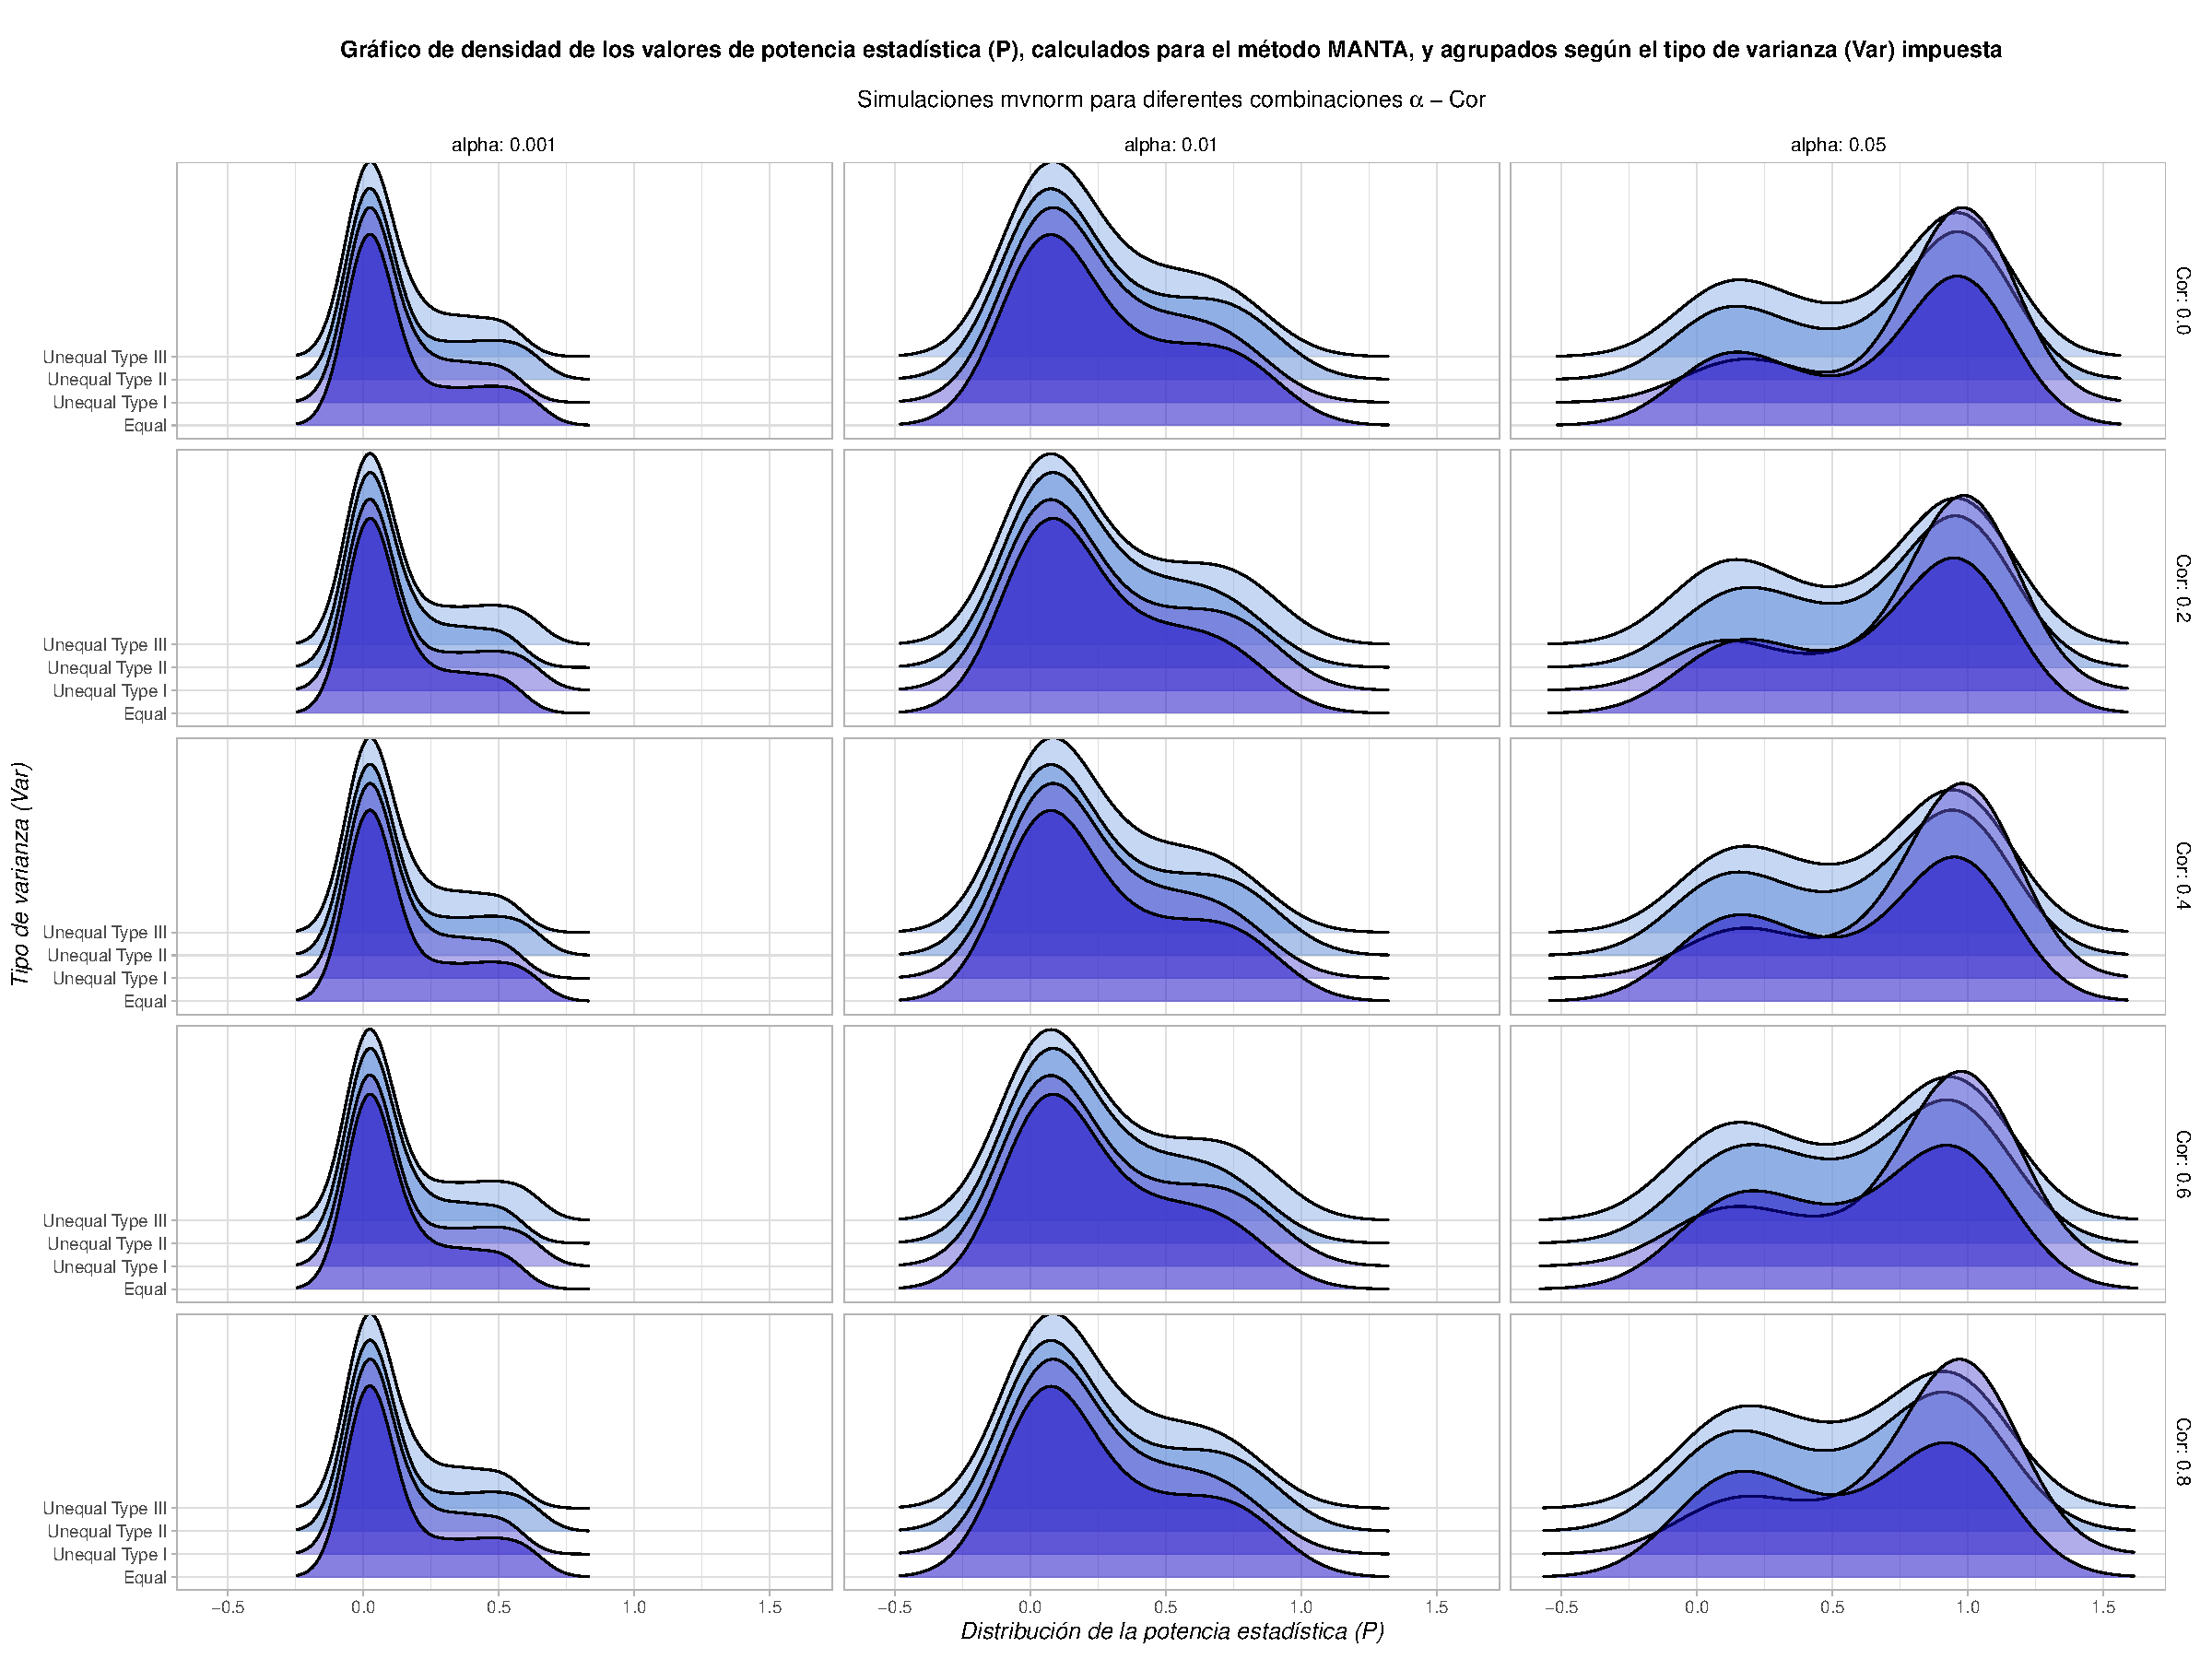
\includegraphics[width = \textwidth]{OBJ1mvnormStatsHomogMANTACorAlpha.pdf}
\caption{OBJ1mvnormStatsHomogMANTACorAlpha}
\label{fig:OBJ1mvnormStatsHomogMANTACorAlpha}
\end{subfigure}
\begin{subfigure}{0.49\textwidth}
\centering
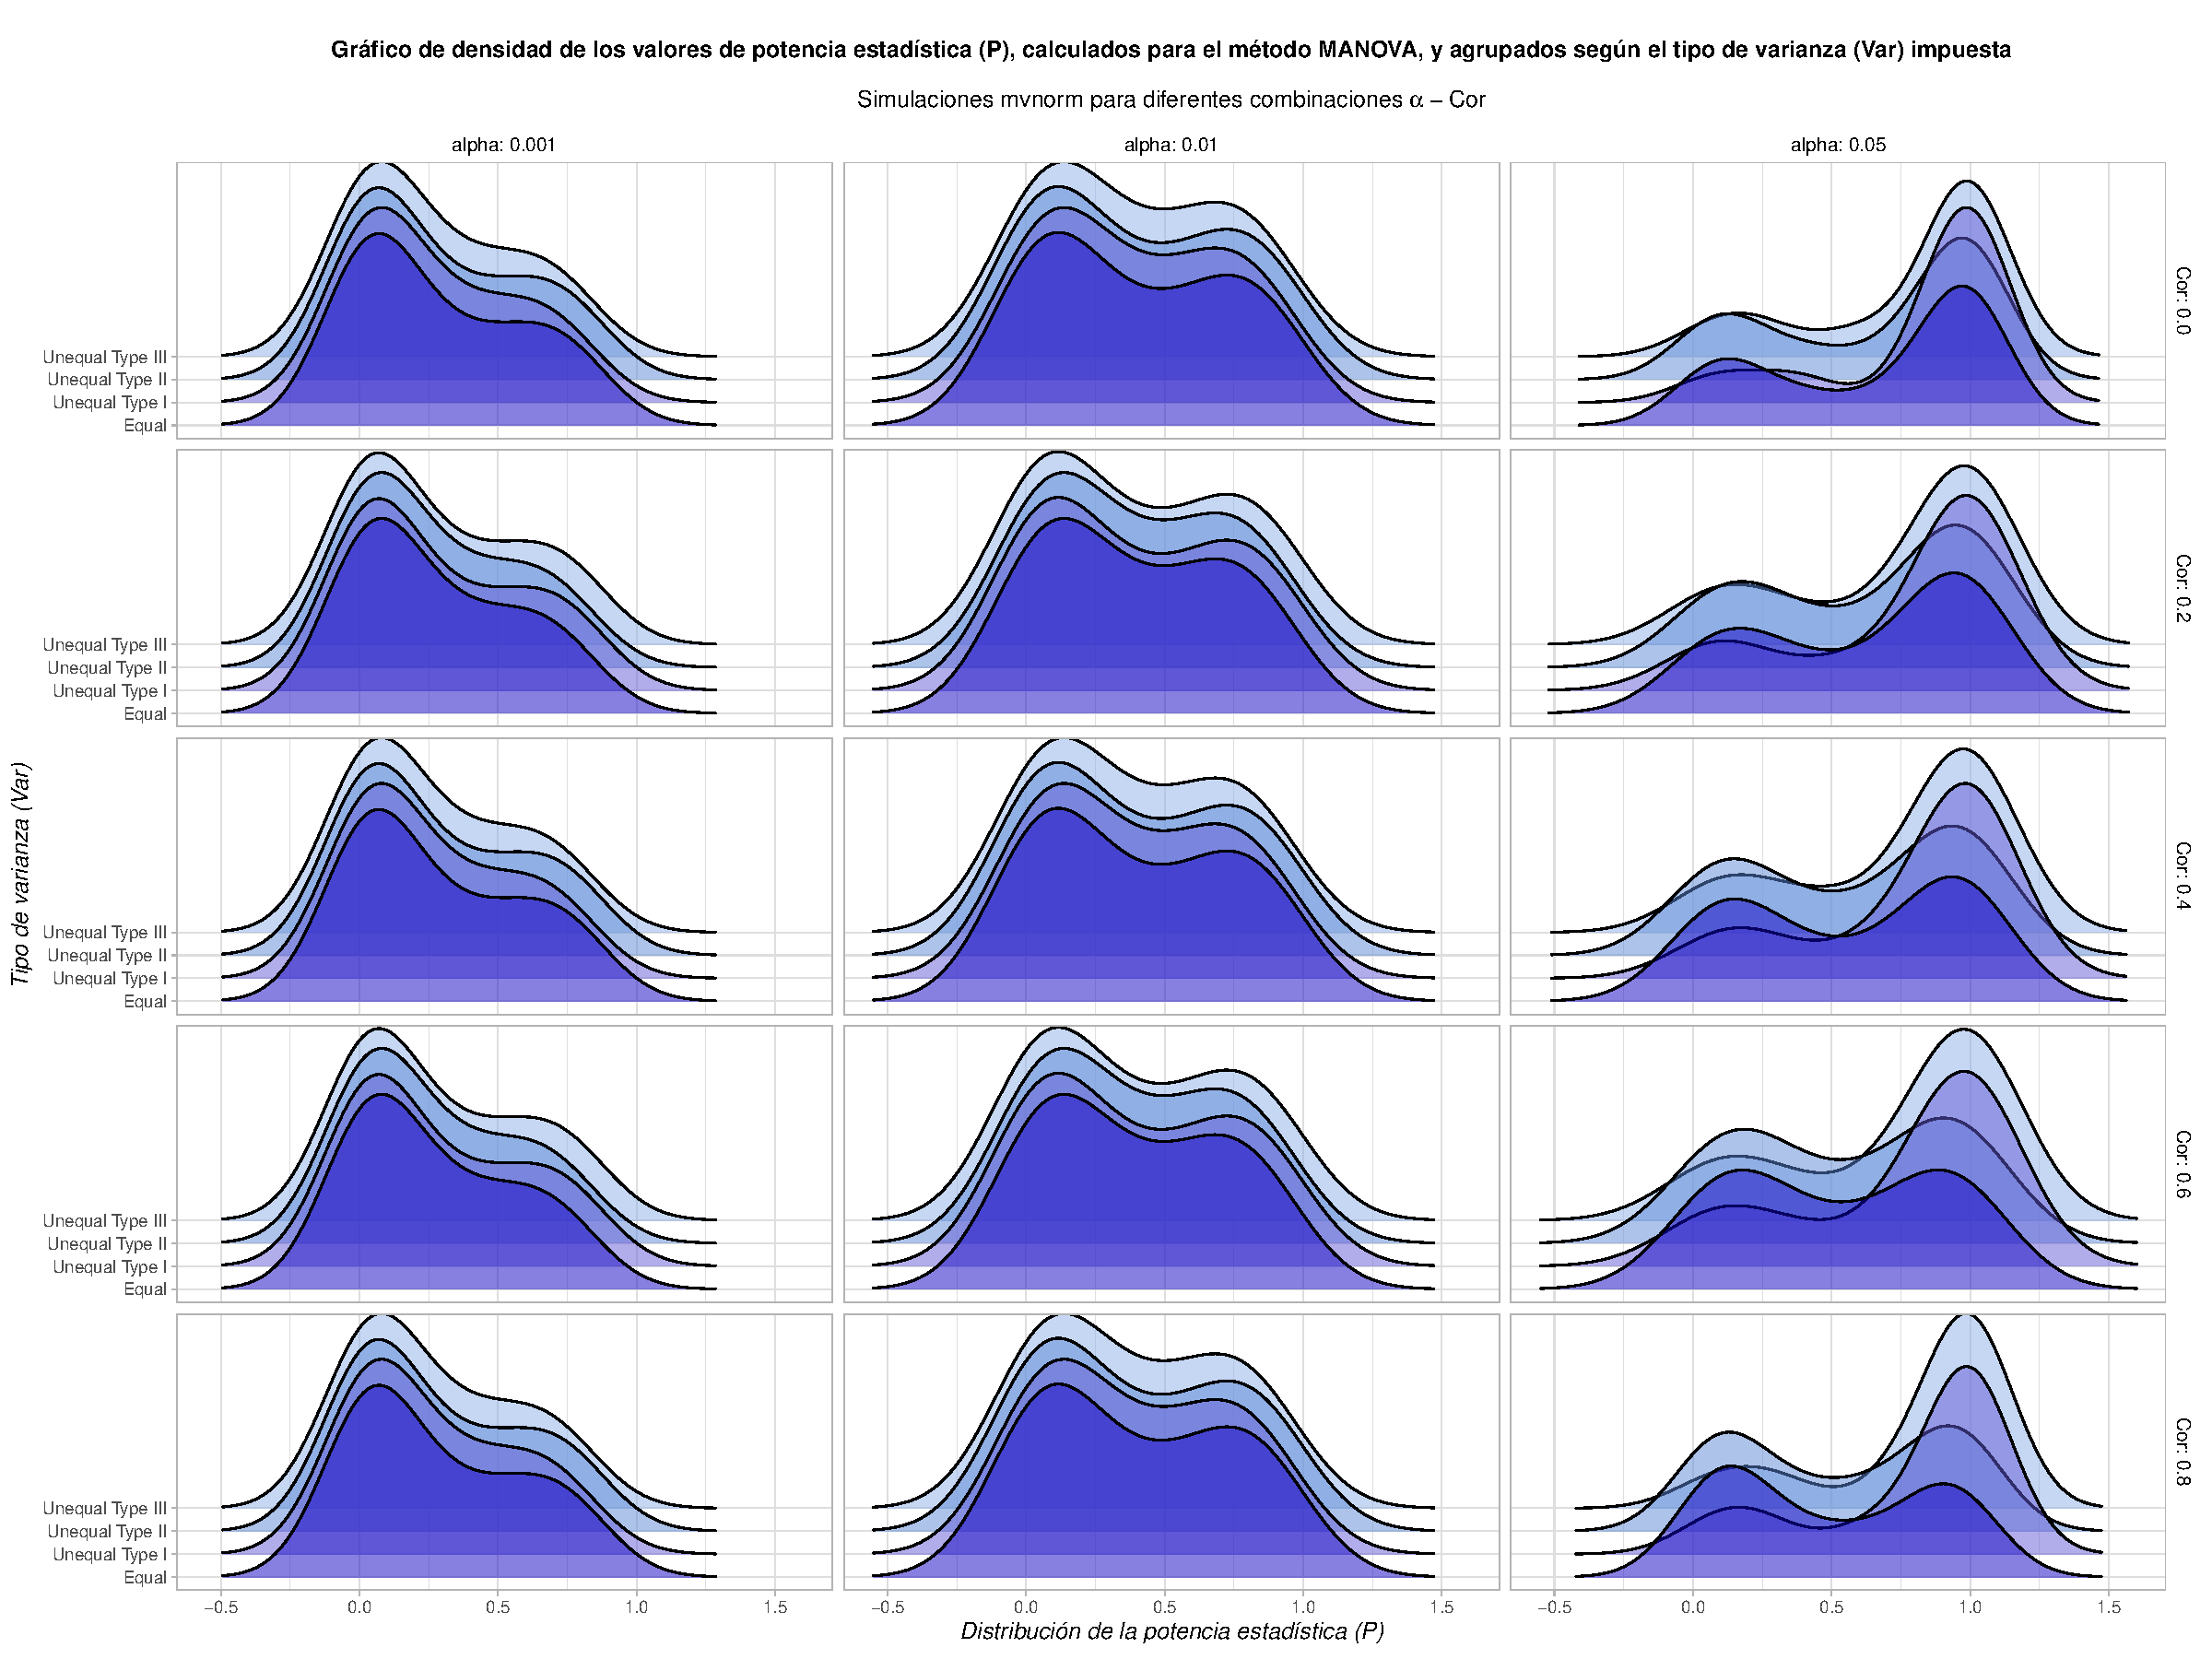
\includegraphics[width = \textwidth]{OBJ1mvnormStatsHomogMANOVACorAlpha.pdf}
\caption{OBJ1mvnormStatsHomogMANOVACorAlpha}
\label{fig:OBJ1mvnormStatsHomogMANOVACorAlpha}
\end{subfigure}
\\
\begin{subfigure}{0.49\textwidth}
\centering
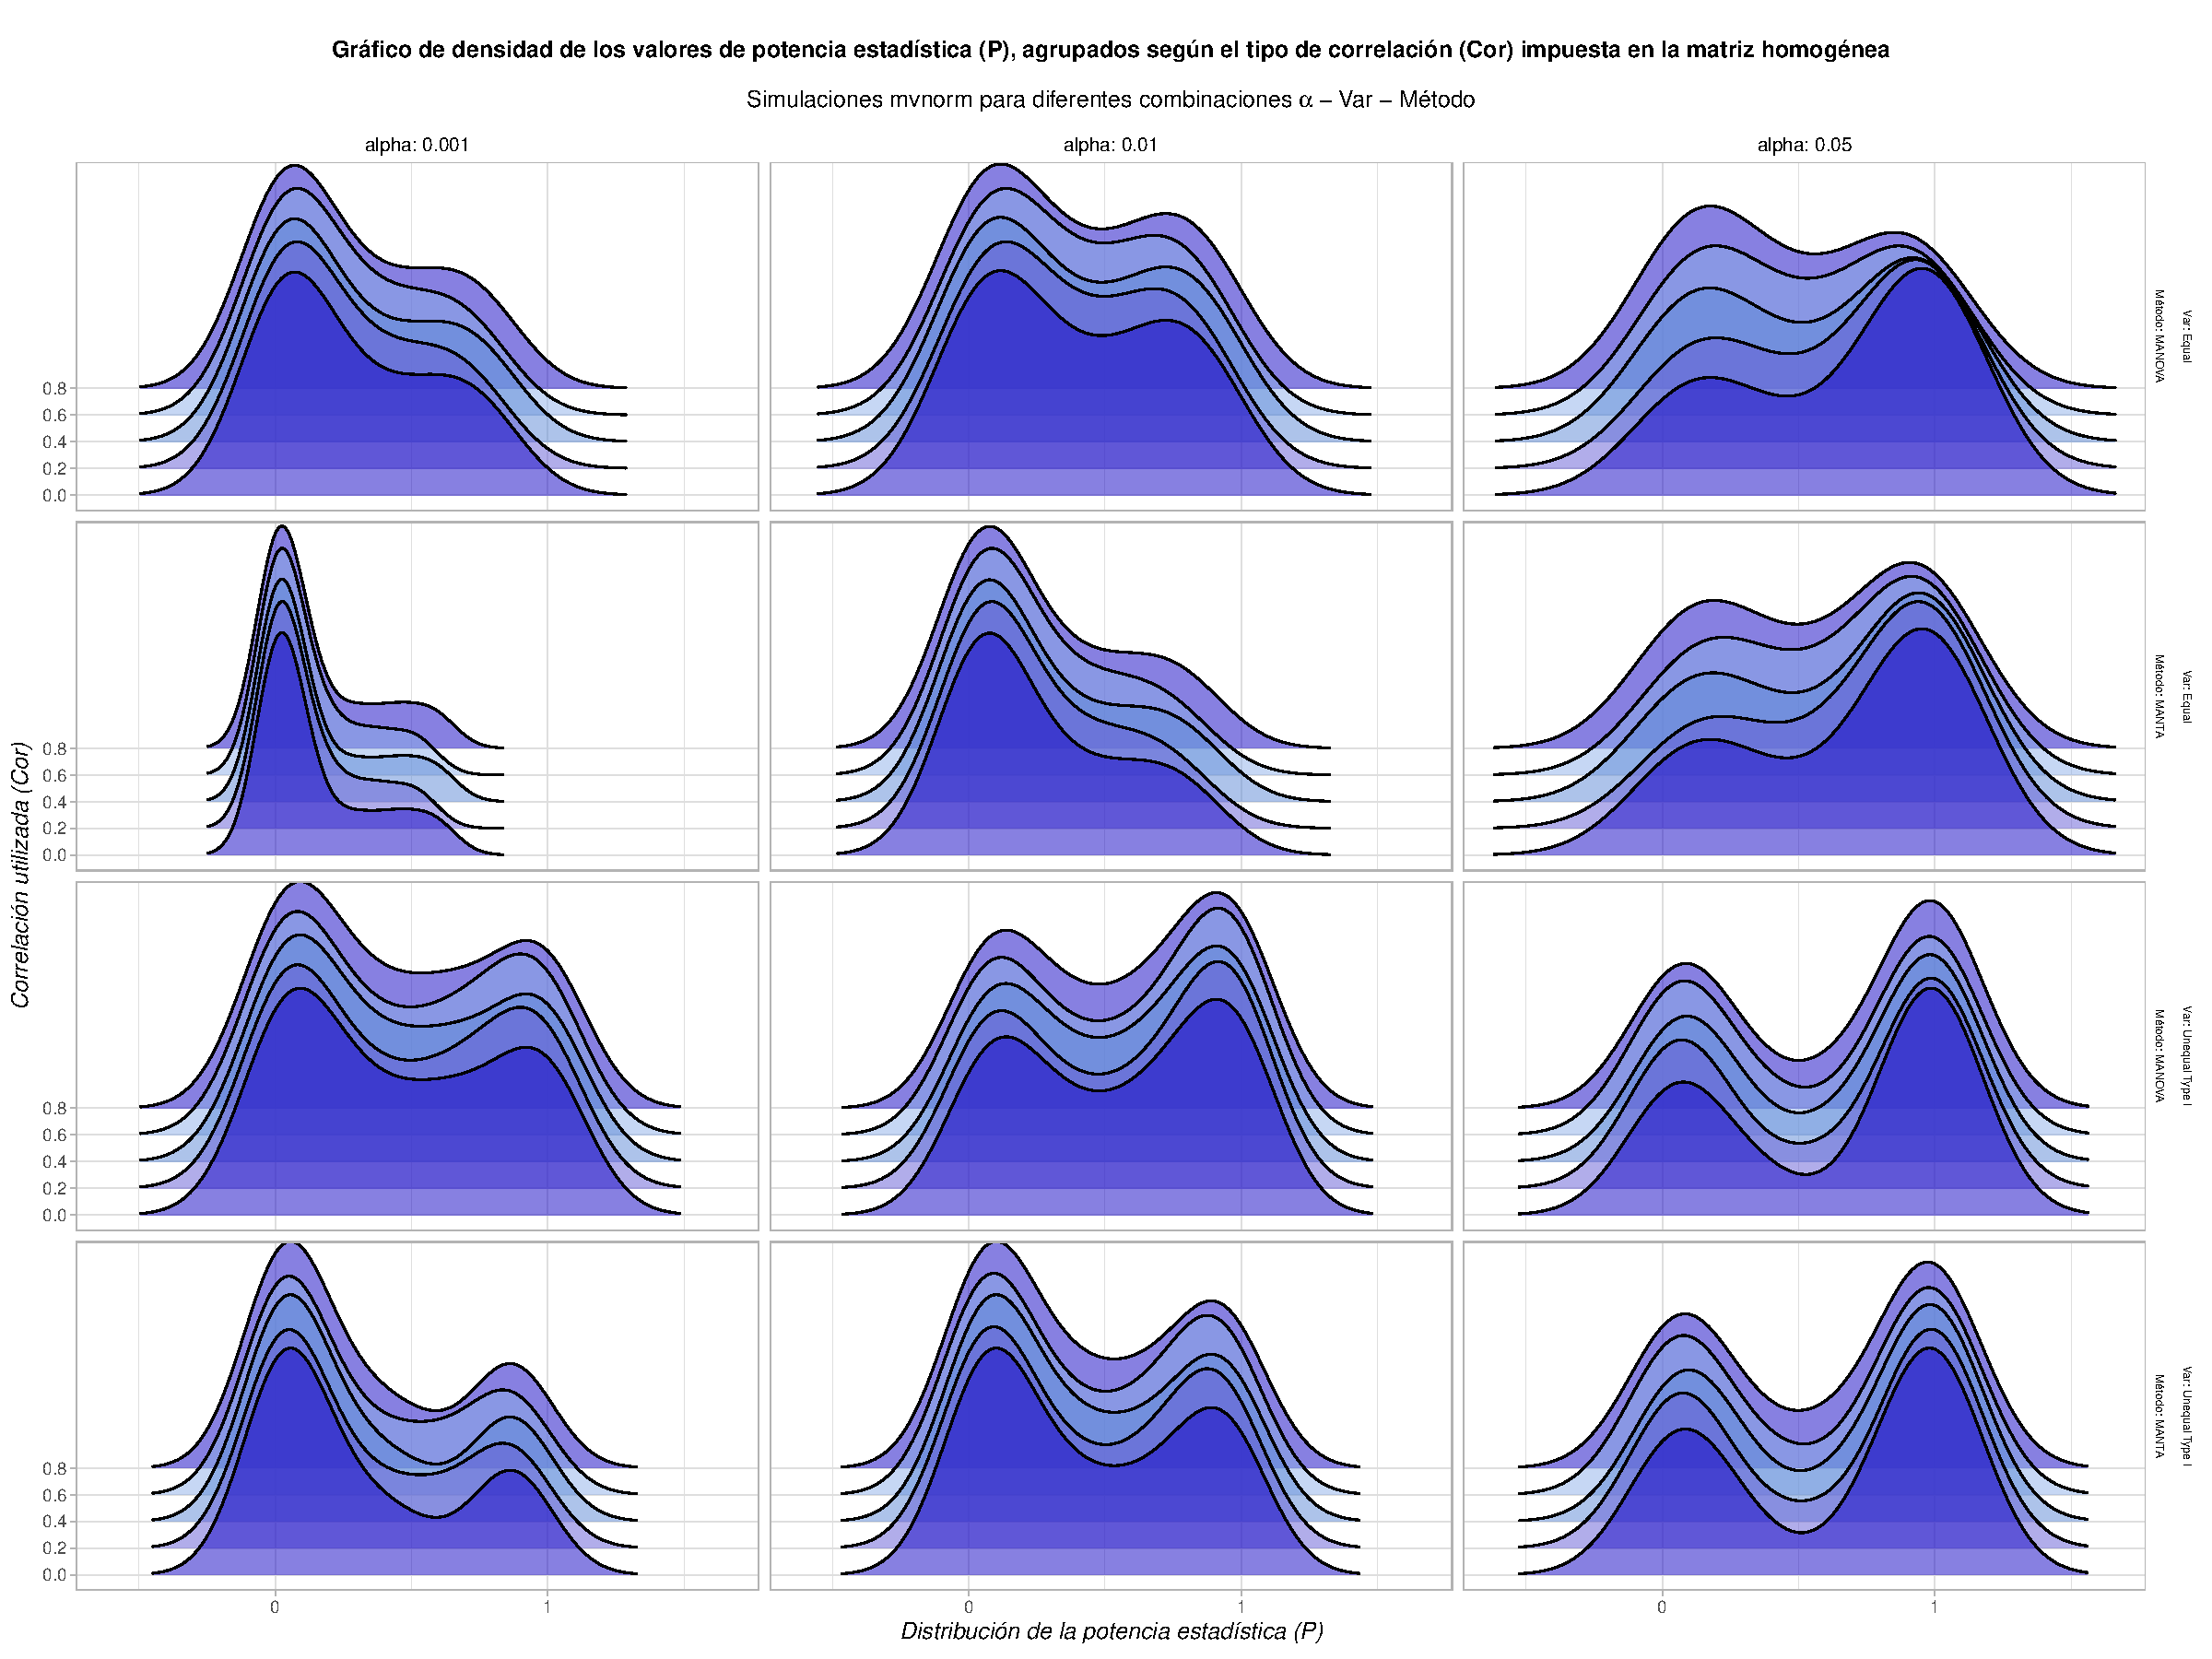
\includegraphics[width = \textwidth]{OBJ1mvnormStatsHomogMANTAMANOVAVar1.pdf}
\caption{OBJ1mvnormStatsHomogMANTAMANOVAVar1}
\label{fig:OBJ1mvnormStatsHomogMANTAMANOVAVar1}
\end{subfigure}
\begin{subfigure}{0.49\textwidth}
\centering
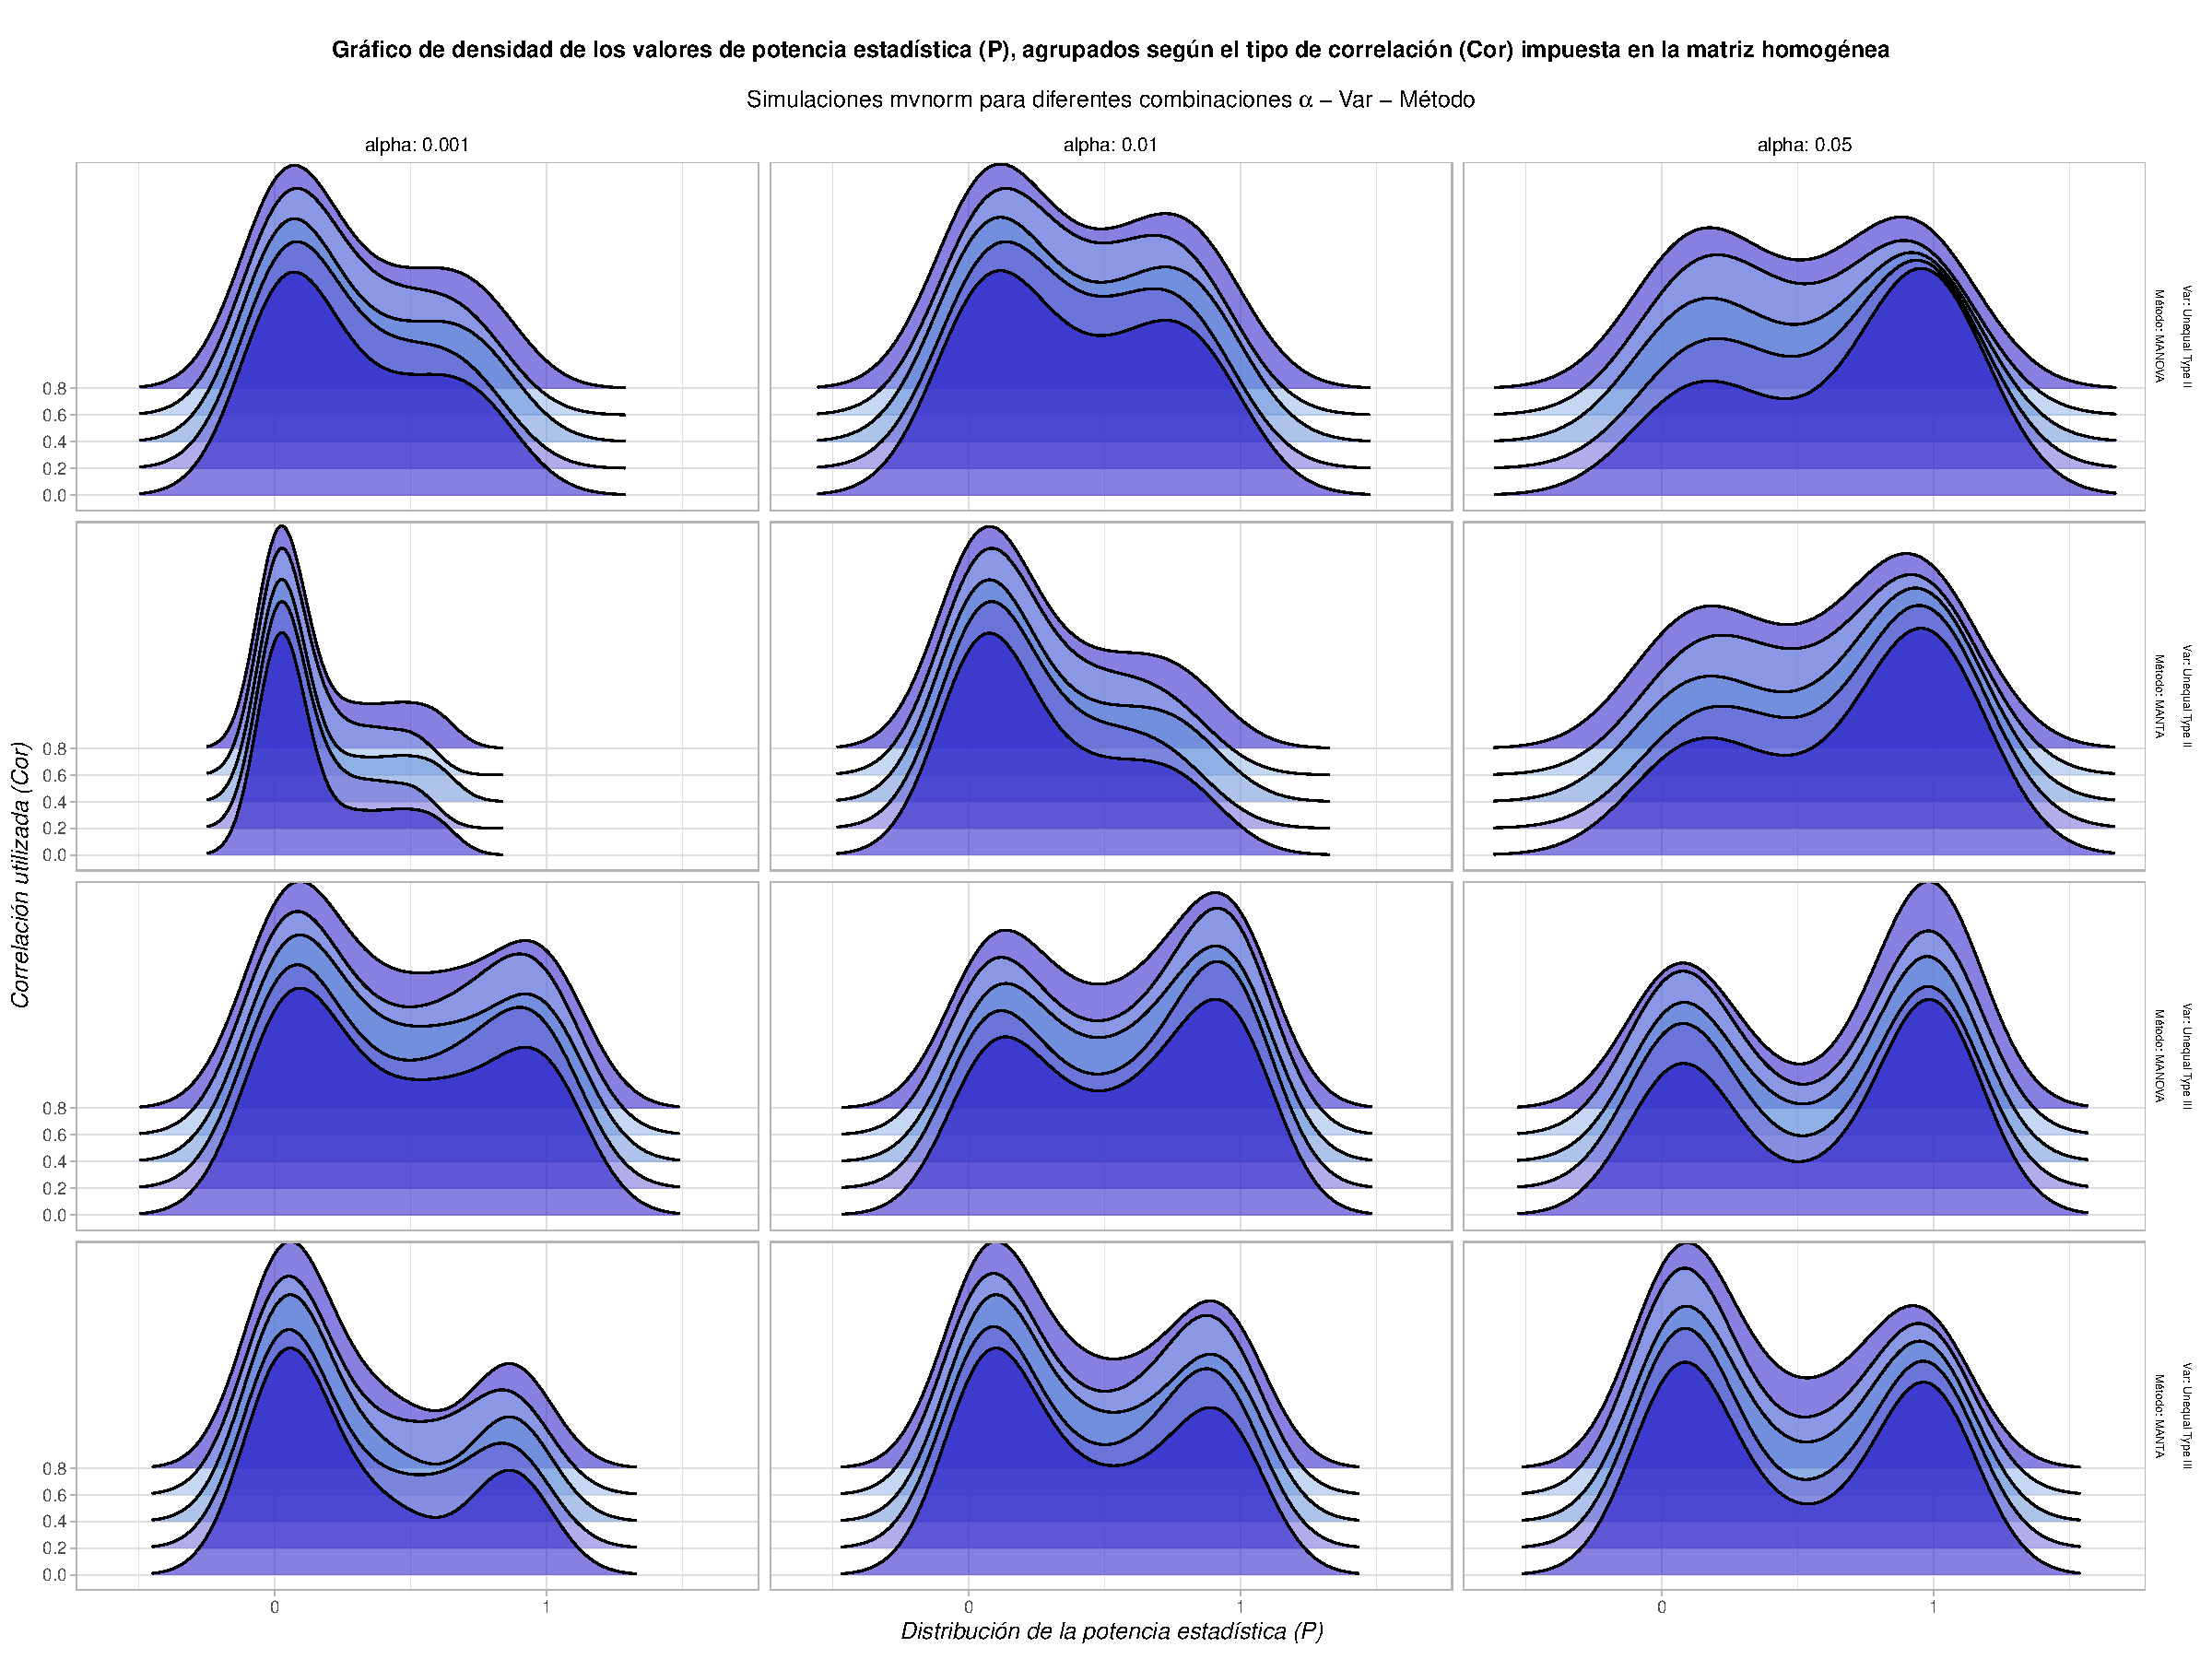
\includegraphics[width = \textwidth]{OBJ1mvnormStatsHomogMANTAMANOVAVar2.pdf}
\caption{OBJ1mvnormStatsHomogMANTAMANOVAVar2}
\label{fig:OBJ1mvnormStatsHomogMANTAMANOVAVar2}
\end{subfigure}
\caption{OBJ1mvnormStatsHomog}
\label{fig:OBJ1mvnormStatsHomog}
\end{figure}

Complementariamente, se muestra también para el supuesto alternativo: determinado por el mismo escenario anterior pero con la salvedad de haber forzado la aplicación de una matriz de correlación \textit{inhomogénea}, con valores aleatorios de la variable \textit{Cor} fuera de la diagonal.

% mvnorm: Stats Potencia - t comp - Datos sin transformar - No Homogen.
\begin{table}[!htbp] \centering 
  \caption{\scriptsize{Descripción de los estadísticos potencia (\( \mathbb P \)) y 
  tiempo de computación (\textit{t comp.}), para los métodos \textbf{MANTA} y 
  \textbf{MANOVA}, bajo una distribución \textit{mvnorm}, con una matriz de correlación 
  \textit{inhomogénea}, y considerando diferentes niveles de significación.}}
  \label{tab:mvnormMANTAMANOVAStatsNOHomoNoTransfAlphas}
% \hspace*{-2cm} % Movimiento relativo del gráfico
\begin{subtable}[t]{0.55\textwidth}
\tiny
\centering
\begin{tabular}{@{\extracolsep{-8pt}}cccccccc} 
\\ \specialrule{.1em}{.05em}{.05em} 
\specialrule{.1em}{.05em}{.05em} 
\multicolumn{1}{c}{Tipo de Datos} & \multicolumn{1}{c}{\( \alpha  \)} & Statistic & \multicolumn{1}{c}{N} & \multicolumn{1}{c}{Mean} & \multicolumn{1}{c}{St. Dev.} & \multicolumn{1}{c}{Min} & \multicolumn{1}{c}{Max} \\ 
\specialrule{.1em}{.05em}{.05em} 
\multirow{6}{*}{Datos sin transformar} & \multirow{2}{*}{0.05} & Potencia & 42 & 0.4257 & 0.3292 & 0.0620 & 0.9550 \\ 
 & & tcomp & 42 & 1.1242 & 0.1114 & 1.0503 & 1.6741 \\ 
 & \multirow{2}{*}{0.01} & Potencia & 42 & 0.2722 & 0.2822 & 0.0140 & 0.8280 \\ 
 & & tcomp & 42 & 1.1125 & 0.0759 & 1.0149 & 1.2862 \\ 
 & \multirow{2}{*}{0.001} & Potencia & 42 & 0.1373 & 0.1862 & 0.0030 & 0.5840 \\ 
 & & tcomp & 42 & 1.0848 & 0.0625 & 1.0200 & 1.3337 \\  
\specialrule{.1em}{.05em}{.05em}   
\end{tabular}
\caption{Método \textbf{MANTA}.}
\label{mvnormMANTAMANOVAStatsNOHomoNoTransfAlphasa}
\end{subtable}
\hfil
\begin{subtable}[t]{0.55\textwidth}
\tiny
\centering
\begin{tabular}{@{\extracolsep{-8pt}}cccccccc} 
\\ \specialrule{.1em}{.05em}{.05em} 
\specialrule{.1em}{.05em}{.05em} 
\multicolumn{1}{c}{Tipo de Datos} & \multicolumn{1}{c}{\( \alpha  \)} & Statistic & \multicolumn{1}{c}{N} & \multicolumn{1}{c}{Mean} & \multicolumn{1}{c}{St. Dev.} & \multicolumn{1}{c}{Min} & \multicolumn{1}{c}{Max} \\ 
\specialrule{.1em}{.05em}{.05em} 
\multirow{6}{*}{Datos sin transformar} & \multirow{2}{*}{0.05} & Potencia & 42 & 0.5154 & 0.3346 & 0.0620 & 0.9600 \\ 
 & & tcomp & 42 & 0.7004 & 0.0560 & 0.6452 & 0.9949 \\ 
 & \multirow{2}{*}{0.01} & Potencia & 42 & 0.3979 & 0.3265 & 0.0200 & 0.9000 \\ 
 & & tcomp & 42 & 0.6956 & 0.0416 & 0.6473 & 0.8252 \\ 
 & \multirow{2}{*}{0.001} & Potencia & 42 & 0.2820 & 0.2833 & 0.0020 & 0.7890 \\ 
 & & tcomp & 42 & 0.6897 & 0.0344 & 0.6532 & 0.8221 \\ 
\specialrule{.1em}{.05em}{.05em}   
\end{tabular}
\caption{Método \textbf{MANOVA}.}
\label{mvnormMANTAMANOVAStatsNOHomoNoTransfAlphasb}
\end{subtable}
\end{table}

% OBJ1mvnormStatsNoHomog.pdf 
\begin{figure}[!htbp]
\hspace*{-2.1cm} % Movimiento relativo del gráfico
    \centering
    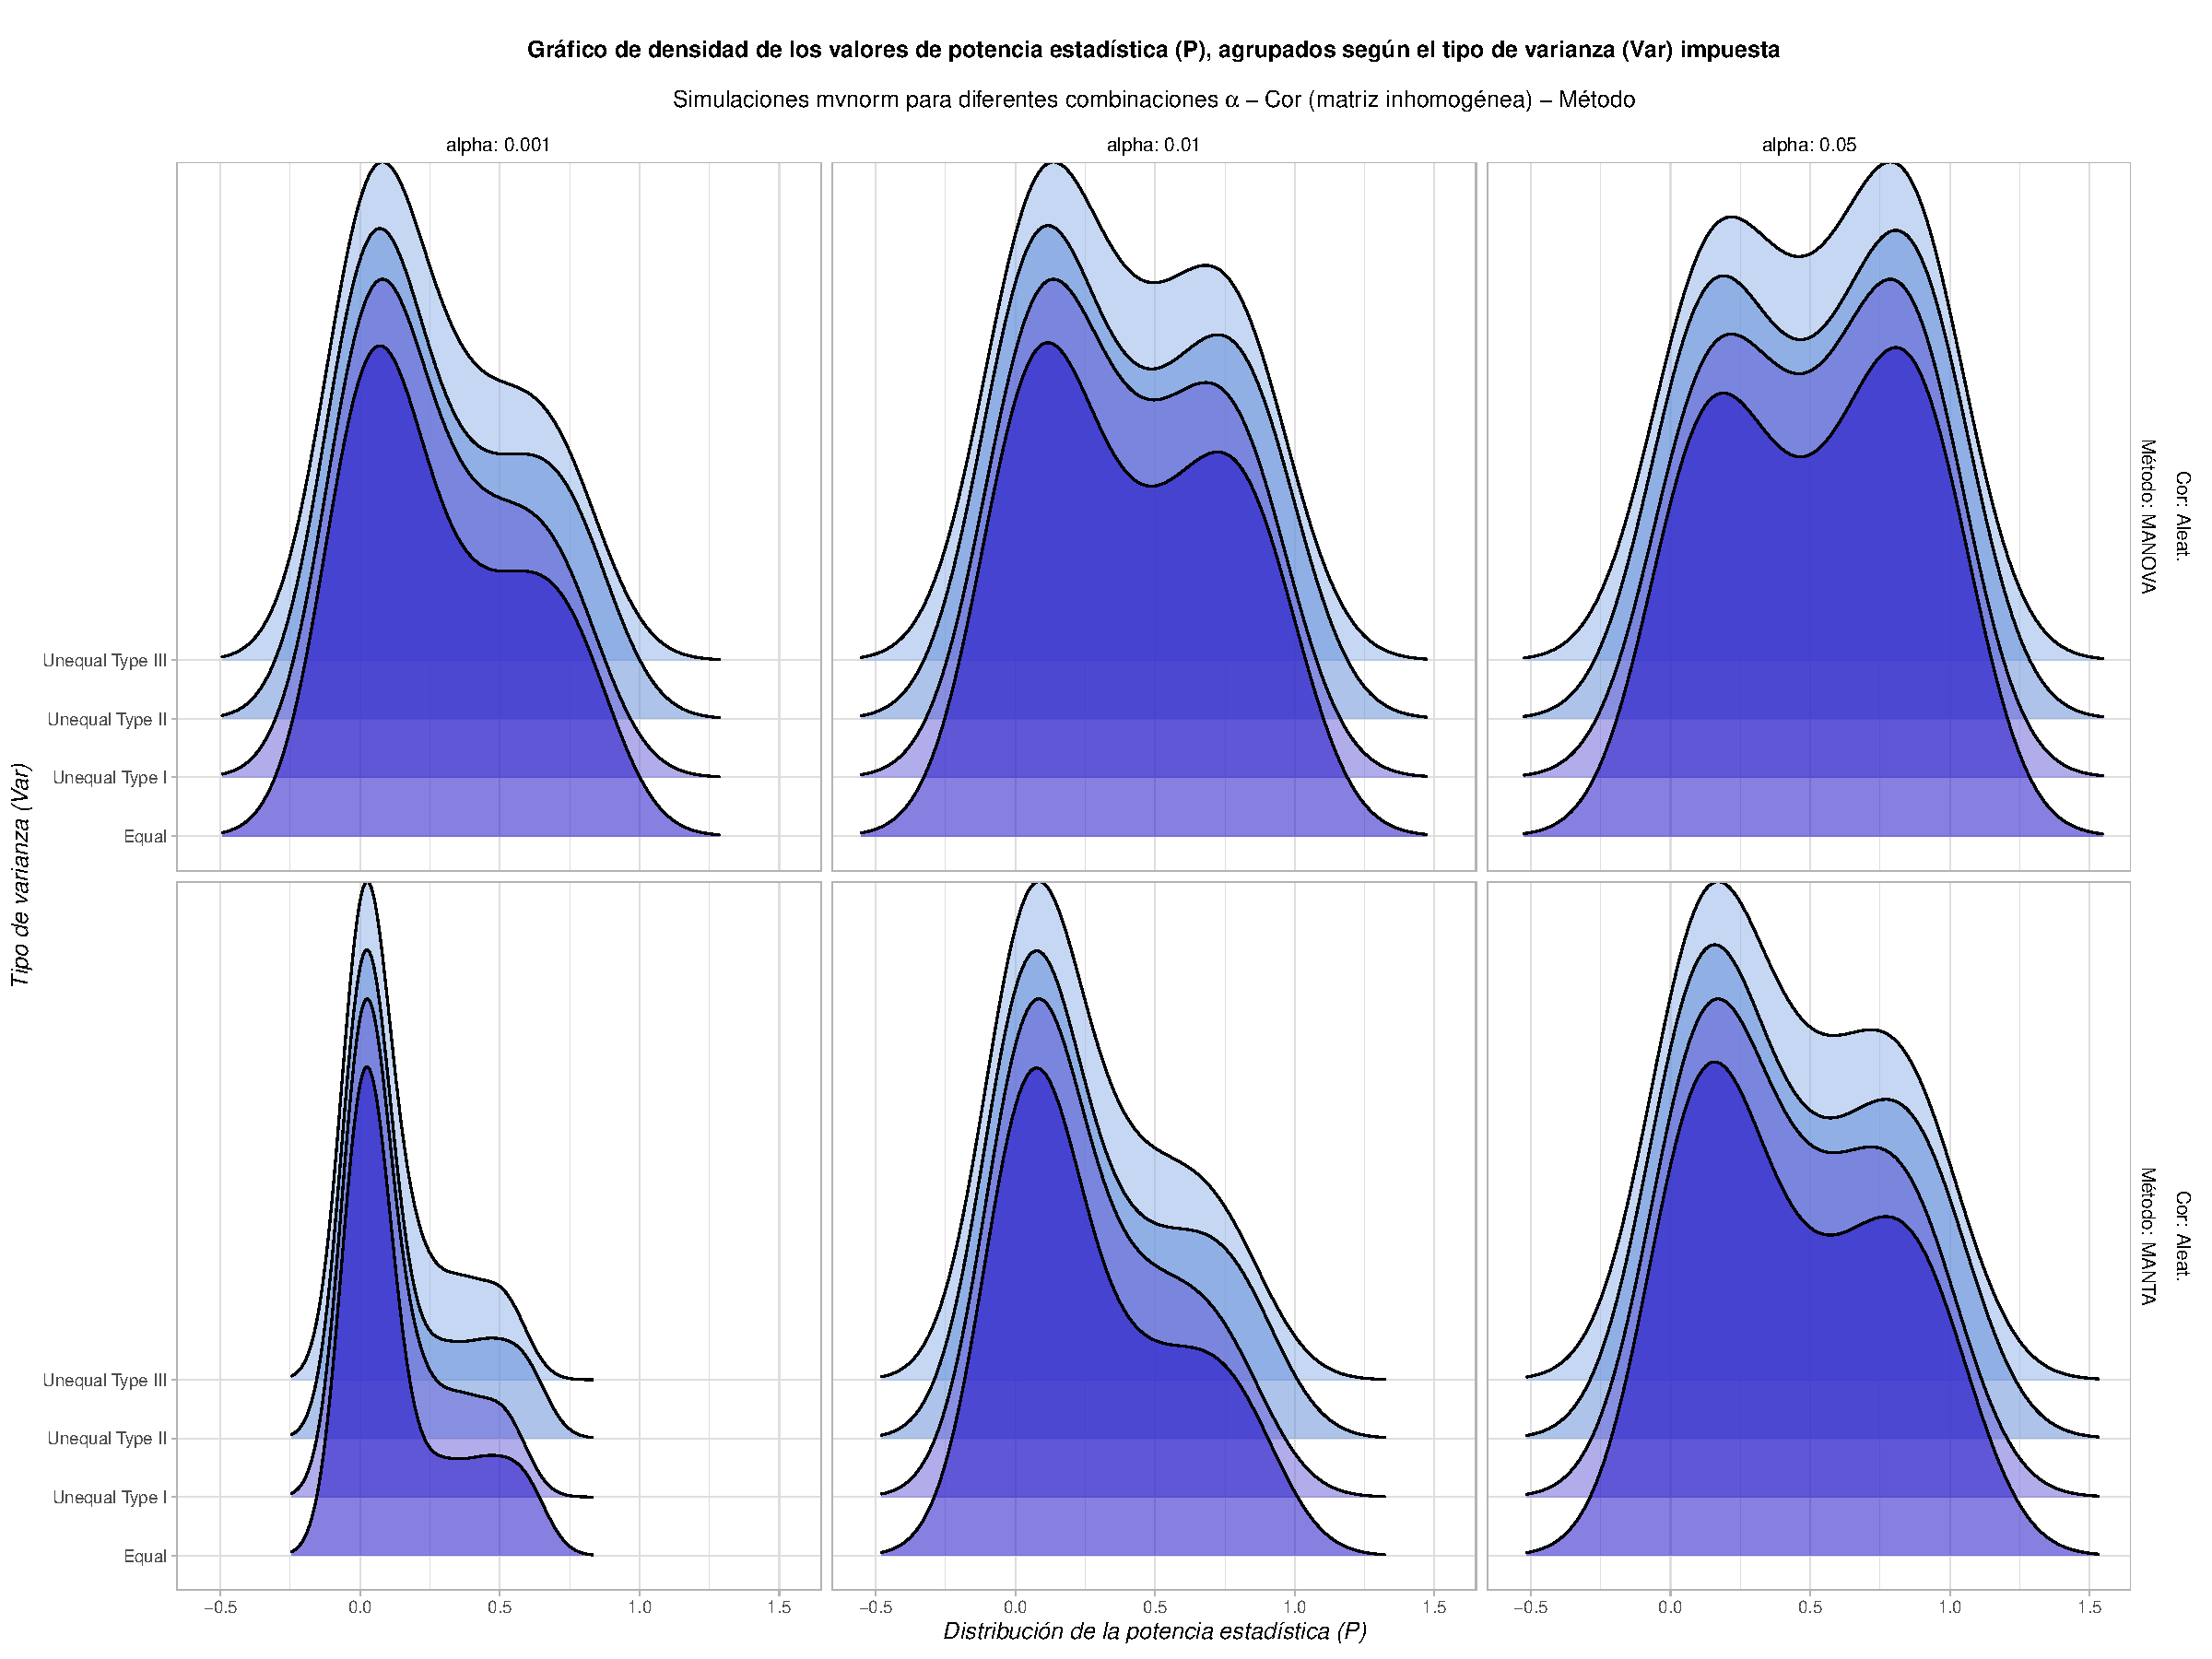
\includegraphics[scale=.3]{OBJ1mvnormStatsNoHomog.pdf}
    \caption{\scriptsize{A.}}
    \label{fig:OBJ1mvnormStatsNoHomog}
\end{figure}

Aún a sabiendas de que algunas de las transformaciones que más típicamente se aplican al tratamiento de un conjunto de datos (\textit{logarítmica} o \textit{log-ratio}, \textit{centered log-ratio} o \textit{clr} y \textit{raíz cuadrada}) no garantizan los supuestos de aplicación de los métodos a estudio, en particular de \textit{MANOVA}, se llevaron a cabo las simulaciones pertinentes con el fin de verificar y, si cabe, cuantificar, dicho efecto. Las tablas correspondientes pueden encontrarse en el apéndice de tablas del presente documento (\ref{tabAppend:mvnormStatsMANTAHomoCorDataTypeAlphas}, \ref{tabAppend:mvnormStatsMANOVAHomoCorDataTypeAlphas}, \ref{tabAppend:mvnormMANTAStatsNOHomoCorDataTypeAlphas} y \ref{tabAppend:mvnormMANOVAStatsNOHomoCorDataTypeAlphas}).

Para tratar de interpretar mejor los datos tabulados anteriormente expuestos, se realizarón representaciones gráficas de estos estadísticos en forma de comparativas de distribuciones de densidad, teniendo en cuenta diferentes combinaciones de las variables de simulación involucradas. Estas son complementarias a las tablas presentadas con anterioridad (\ref{fig:?}).





Tras esta exposición, se procederá a mostrar los resultados del estudio comparativo detallado previamente en forma de representaciones de mallas gráficas para las consideraciones del primer punto (\textit{a}) del \textit{Objetivo I}.

% OBJ1a005.pdf
\begin{figure}[!htbp]
% \hspace*{-1.6cm} % Movimiento relativo del gráfico
    \centering
    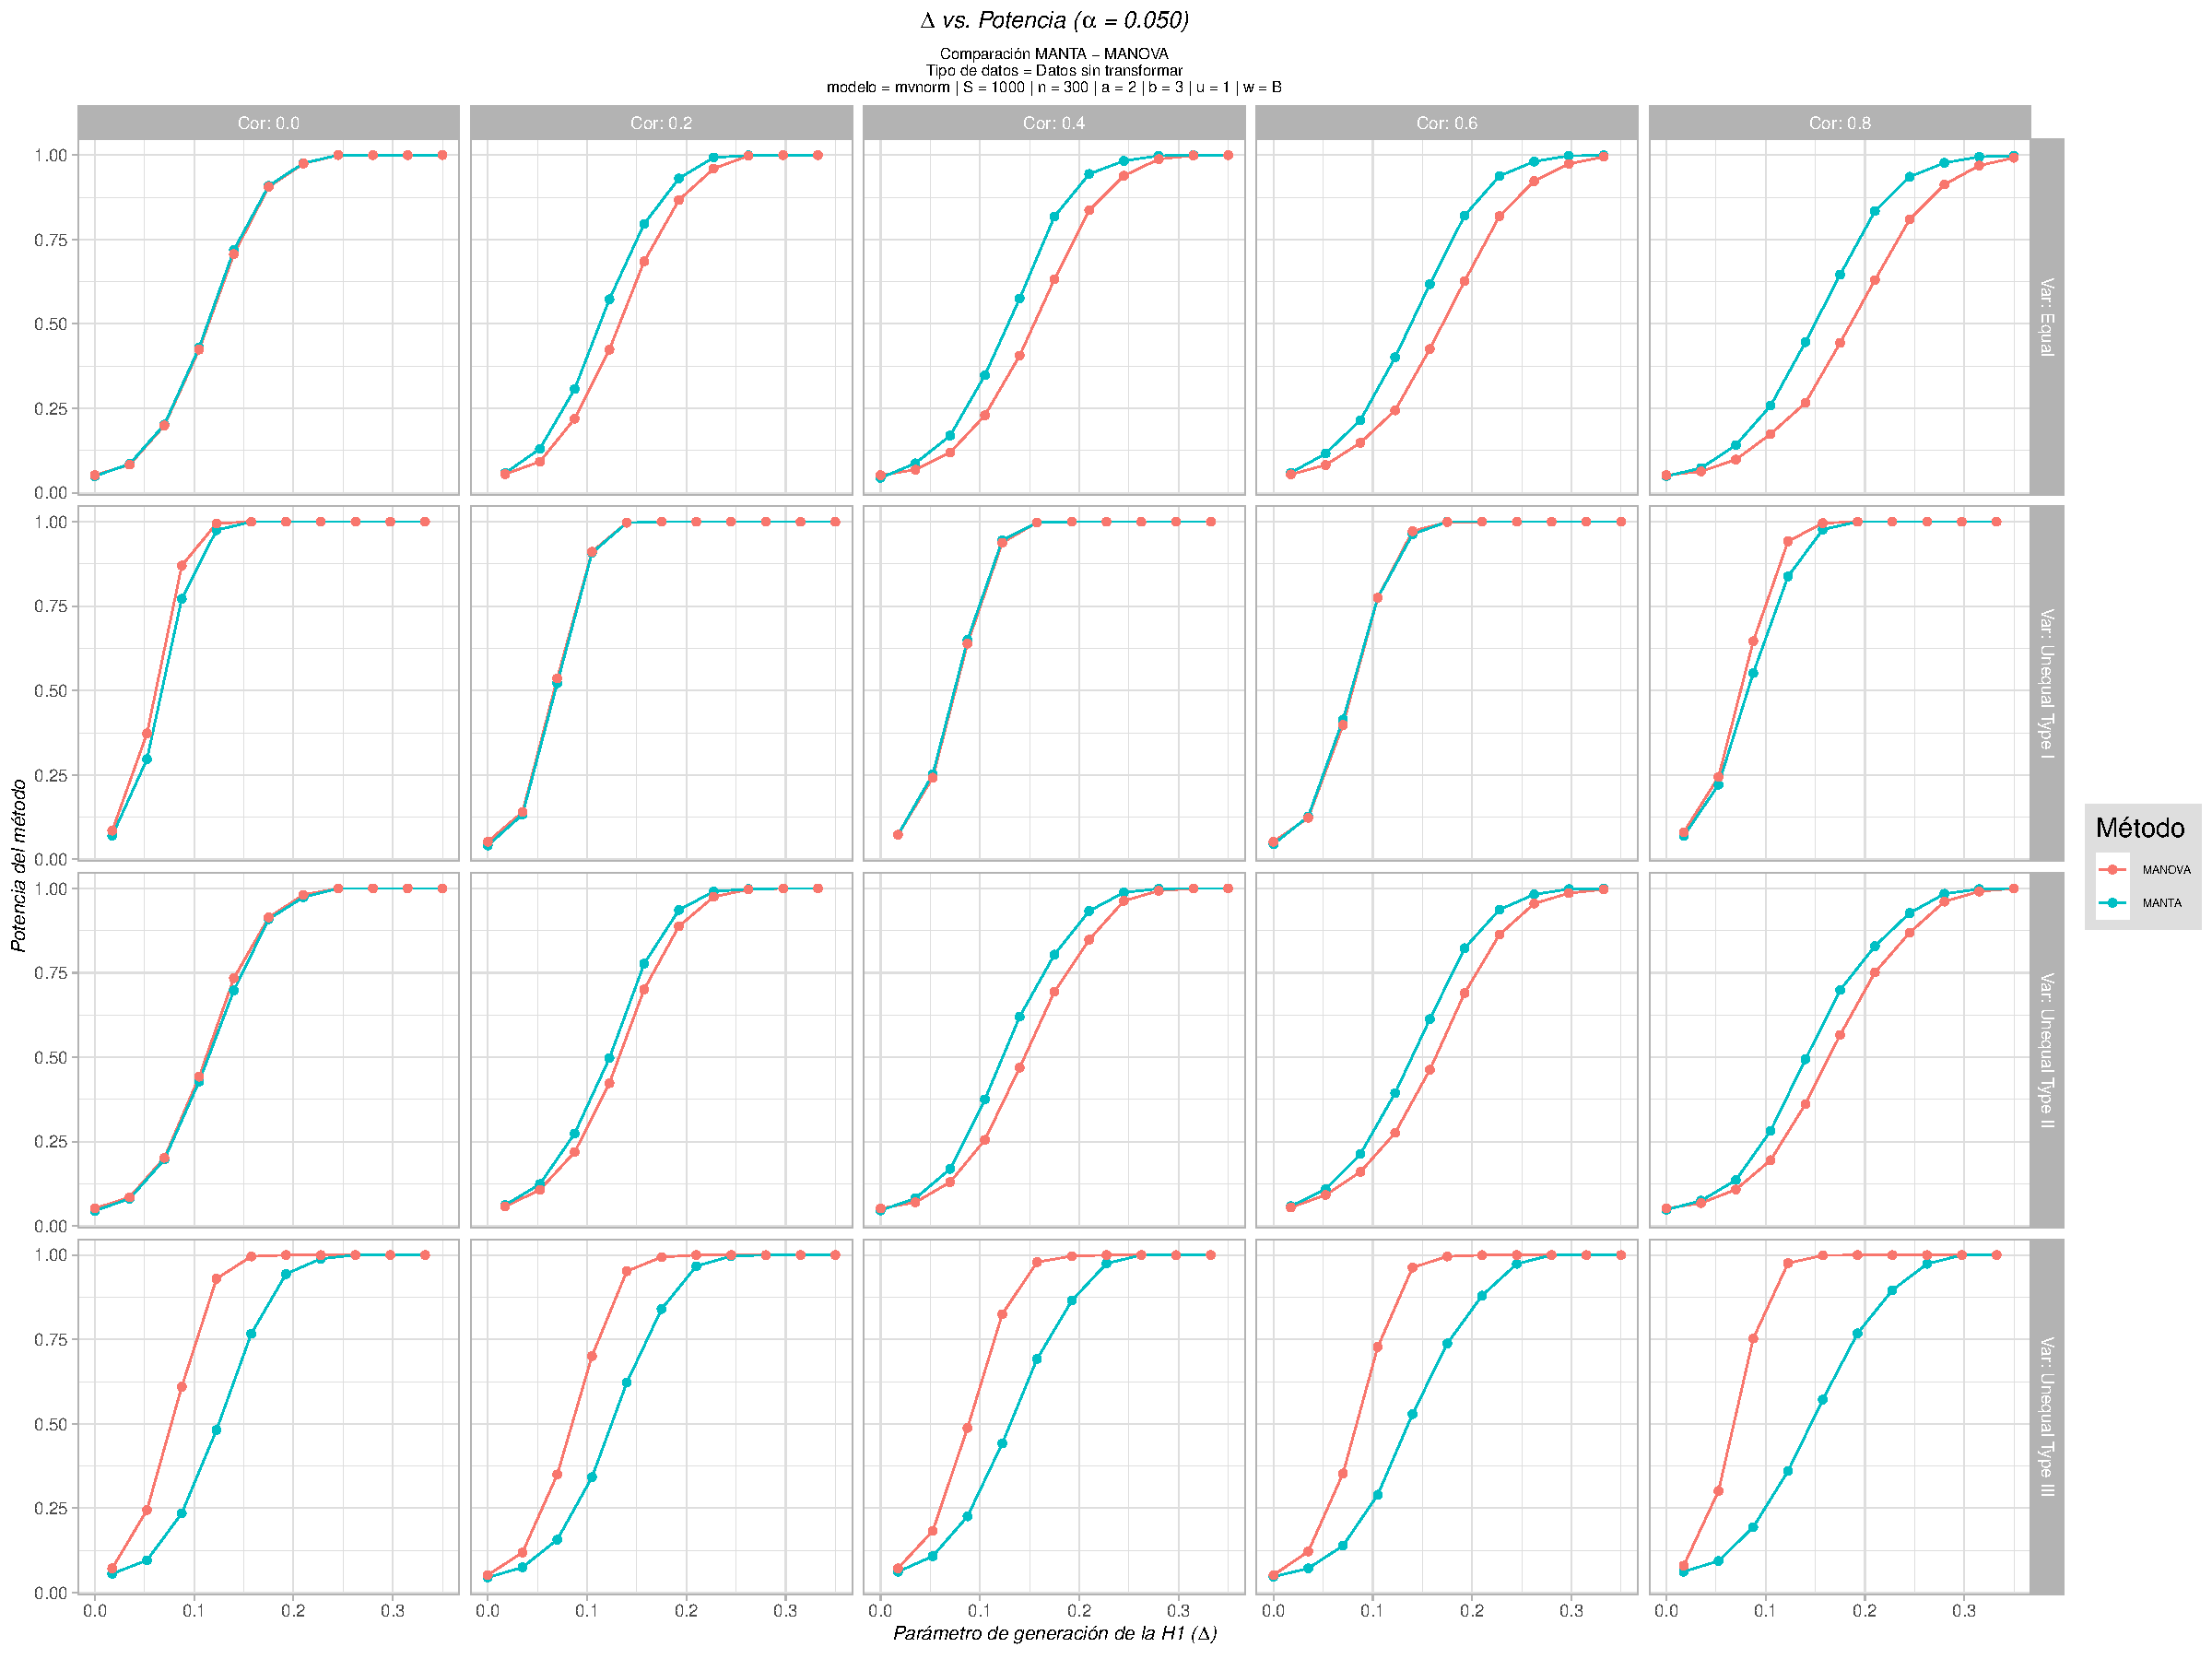
\includegraphics[scale=.45]{OBJ1a005.pdf}
    \caption{\scriptsize{A.}}
    \label{fig:OBJ1a005}
\end{figure}

Seguidamente, se presentan los productos resultantes de las simulaciones pertenecientes al punto \textit{b}.

% OBJ1bALEAT005.pdf
% OBJ1bALEATInvMANTAMANOVA001.pdf
% OBJ1bALEATInvMANTAMANOVA0001.pdf
% OBJ1bALEATInvMANTAMANOVA005.pdf
% OBJ1bHomclr001.pdf
% OBJ1bHomclr0001.pdf
% OBJ1bHomclr005.pdf
% OBJ1bHomInvMANOVA001.pdf
% OBJ1bHomInvMANOVA0001.pdf
% OBJ1bHomInvMANOVA005.pdf
% OBJ1bHomInvMANTA001.pdf
% OBJ1bHomInvMANTA0001.pdf
% OBJ1bHomInvMANTA005.pdf
% OBJ1bHomlog001.pdf
% OBJ1bHomlog0001.pdf
% OBJ1bHomlog005.pdf
% OBJ1bHomNoTransf001.pdf
% OBJ1bHomNoTransf0001.pdf
% OBJ1bHomNoTransf005.pdf
% OBJ1bHomsqrt001.pdf
% OBJ1bHomsqrt0001.pdf
% OBJ1bHomsqrt005.pdf
\begin{figure}[!htbp]
\hspace*{-1.6cm} % Movimiento relativo del gráfico
    \centering
    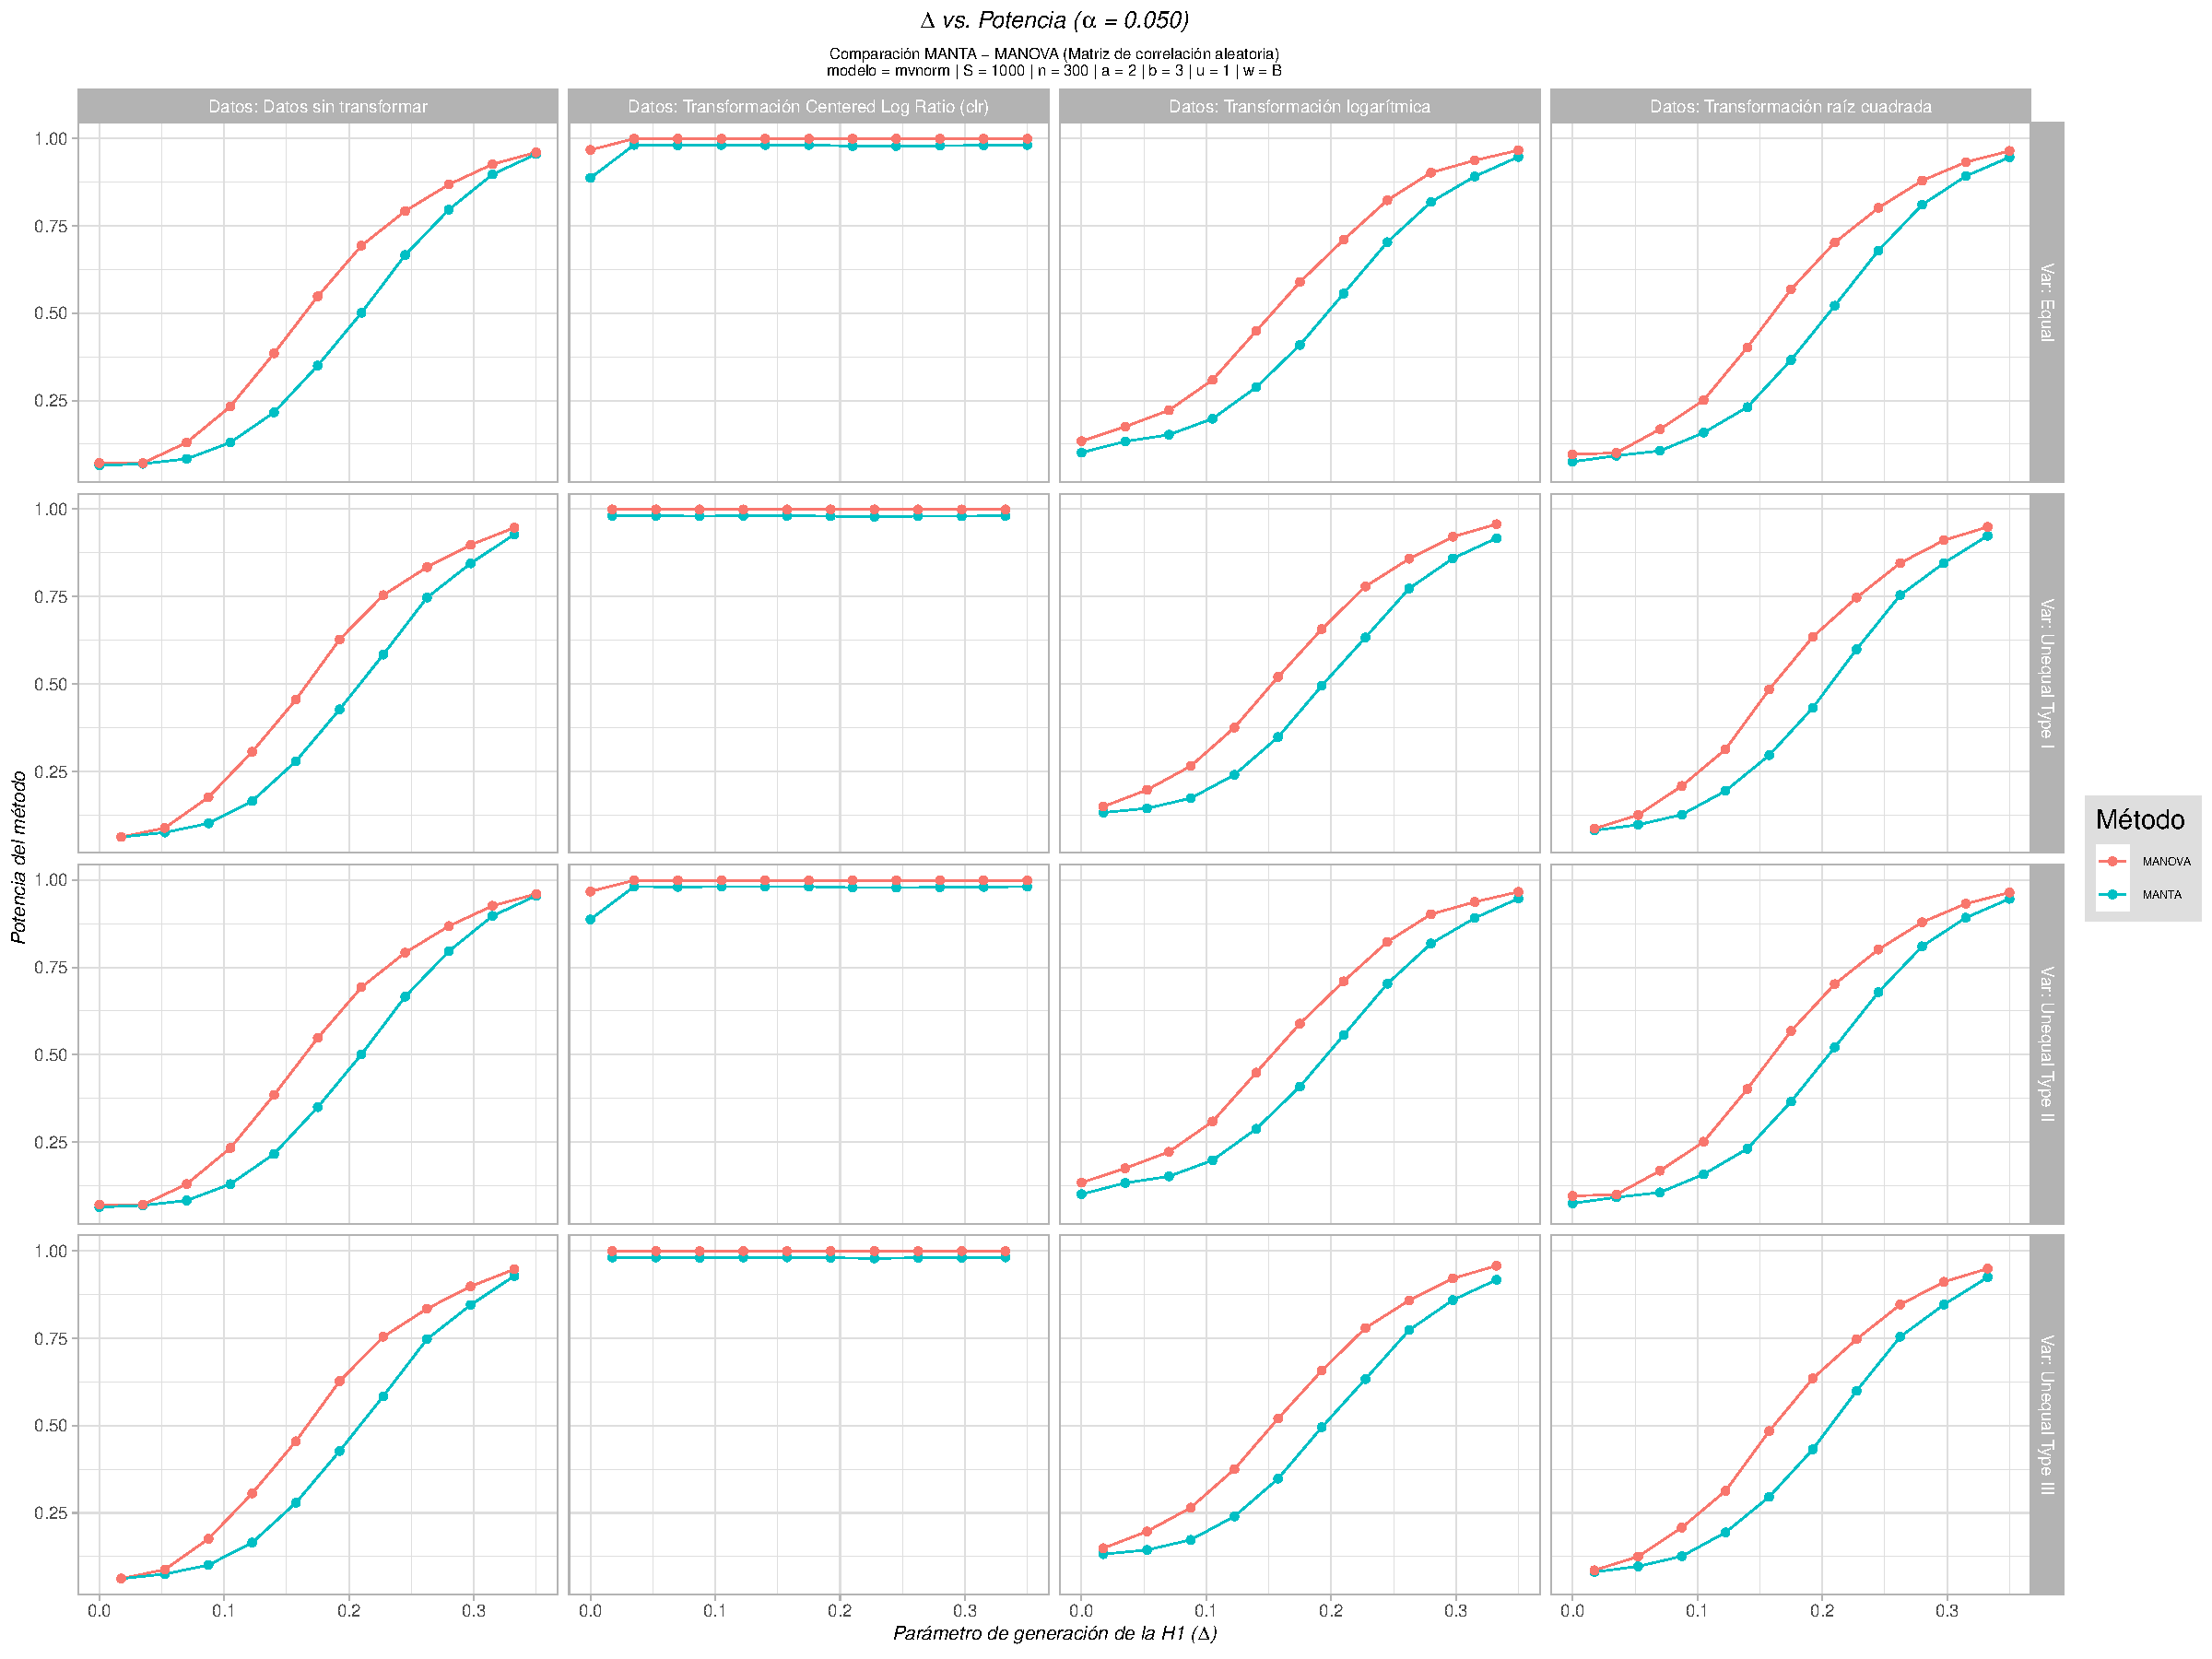
\includegraphics[scale=.51]{OBJ1bALEAT005.pdf}
    \caption{\scriptsize{A.}}
    \label{fig:OBJ1bALEAT005}
\end{figure}

De la misma forma, se añden los resultados gráficos de la computación de los escenarios determinados en \textit{c}.

% OBJ1c1005.pdf
% OBJ1c2001.pdf
% OBJ1c30001.pdf
\begin{figure}[!htbp]
\hspace*{-2cm} % Movimiento relativo del gráfico
\begin{subfigure}{.65\textwidth}
  \centering
  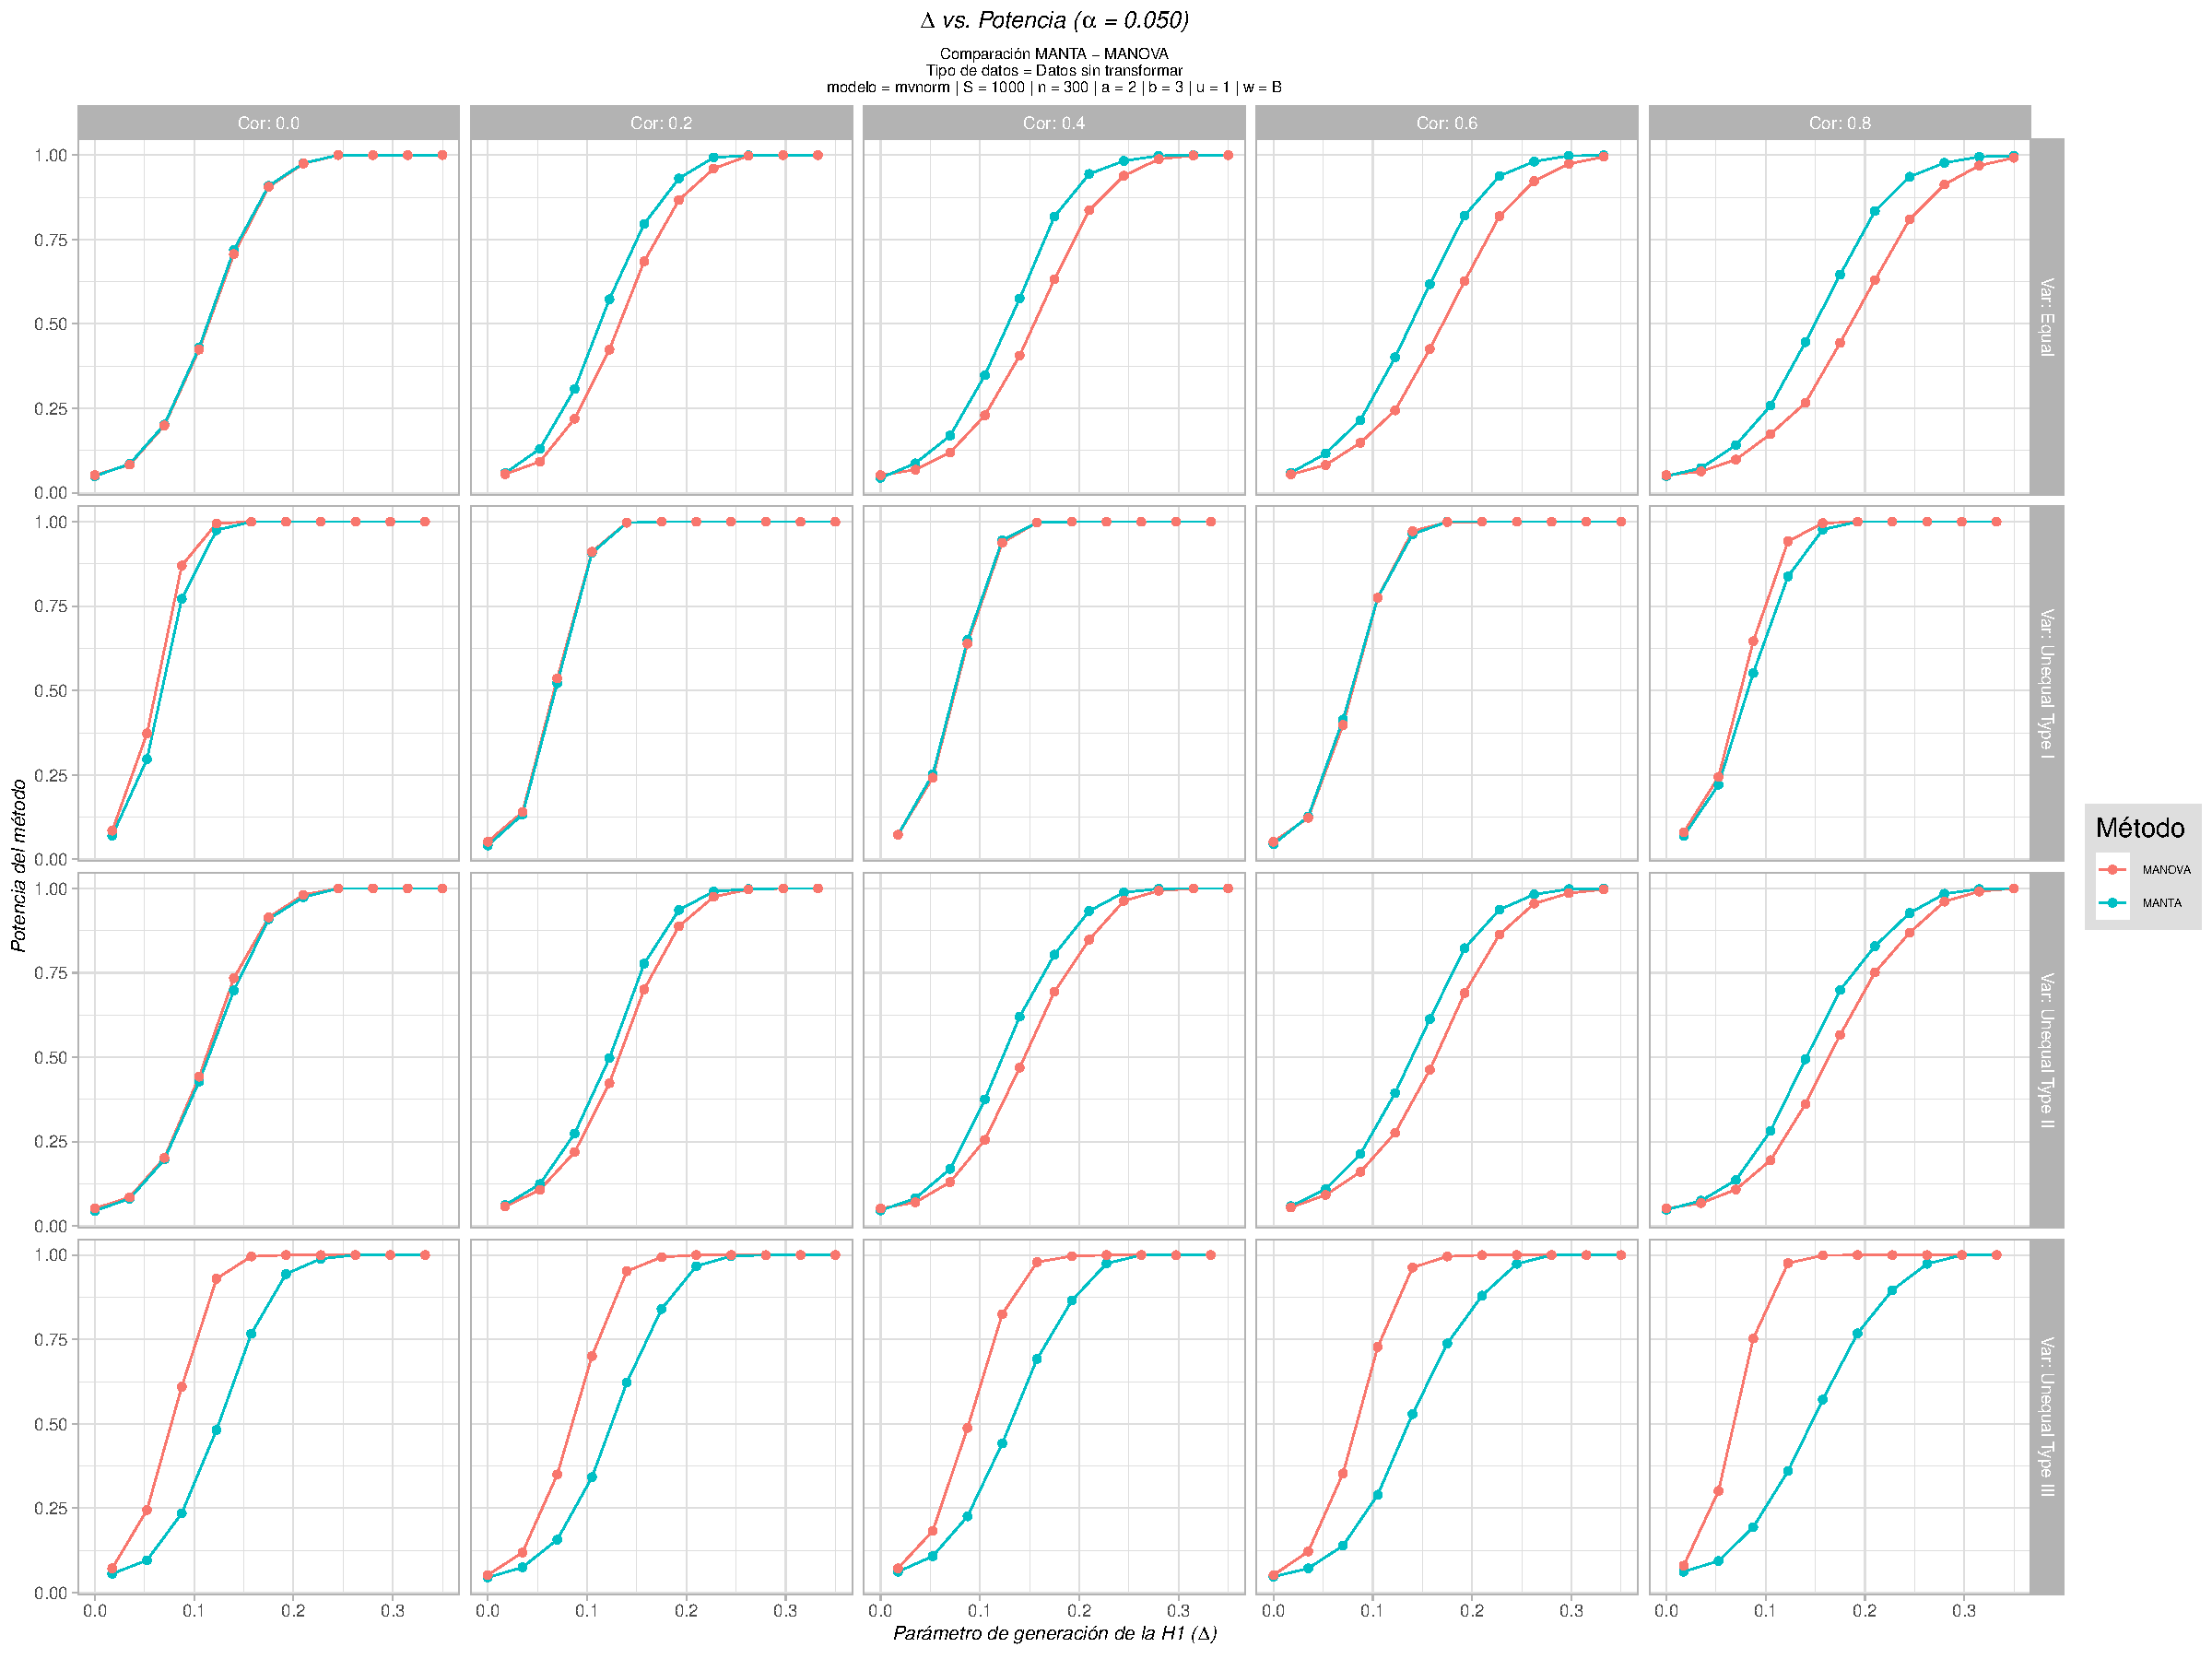
\includegraphics[width=.9\linewidth]{OBJ1c1005.pdf}
  \caption{\scriptsize{A.}}
  \label{fig:OBJ1c1005}
\end{subfigure}%
\begin{subfigure}{.65\textwidth}
\hspace*{-2.3cm} % Movimiento relativo del gráfico
  \centering
  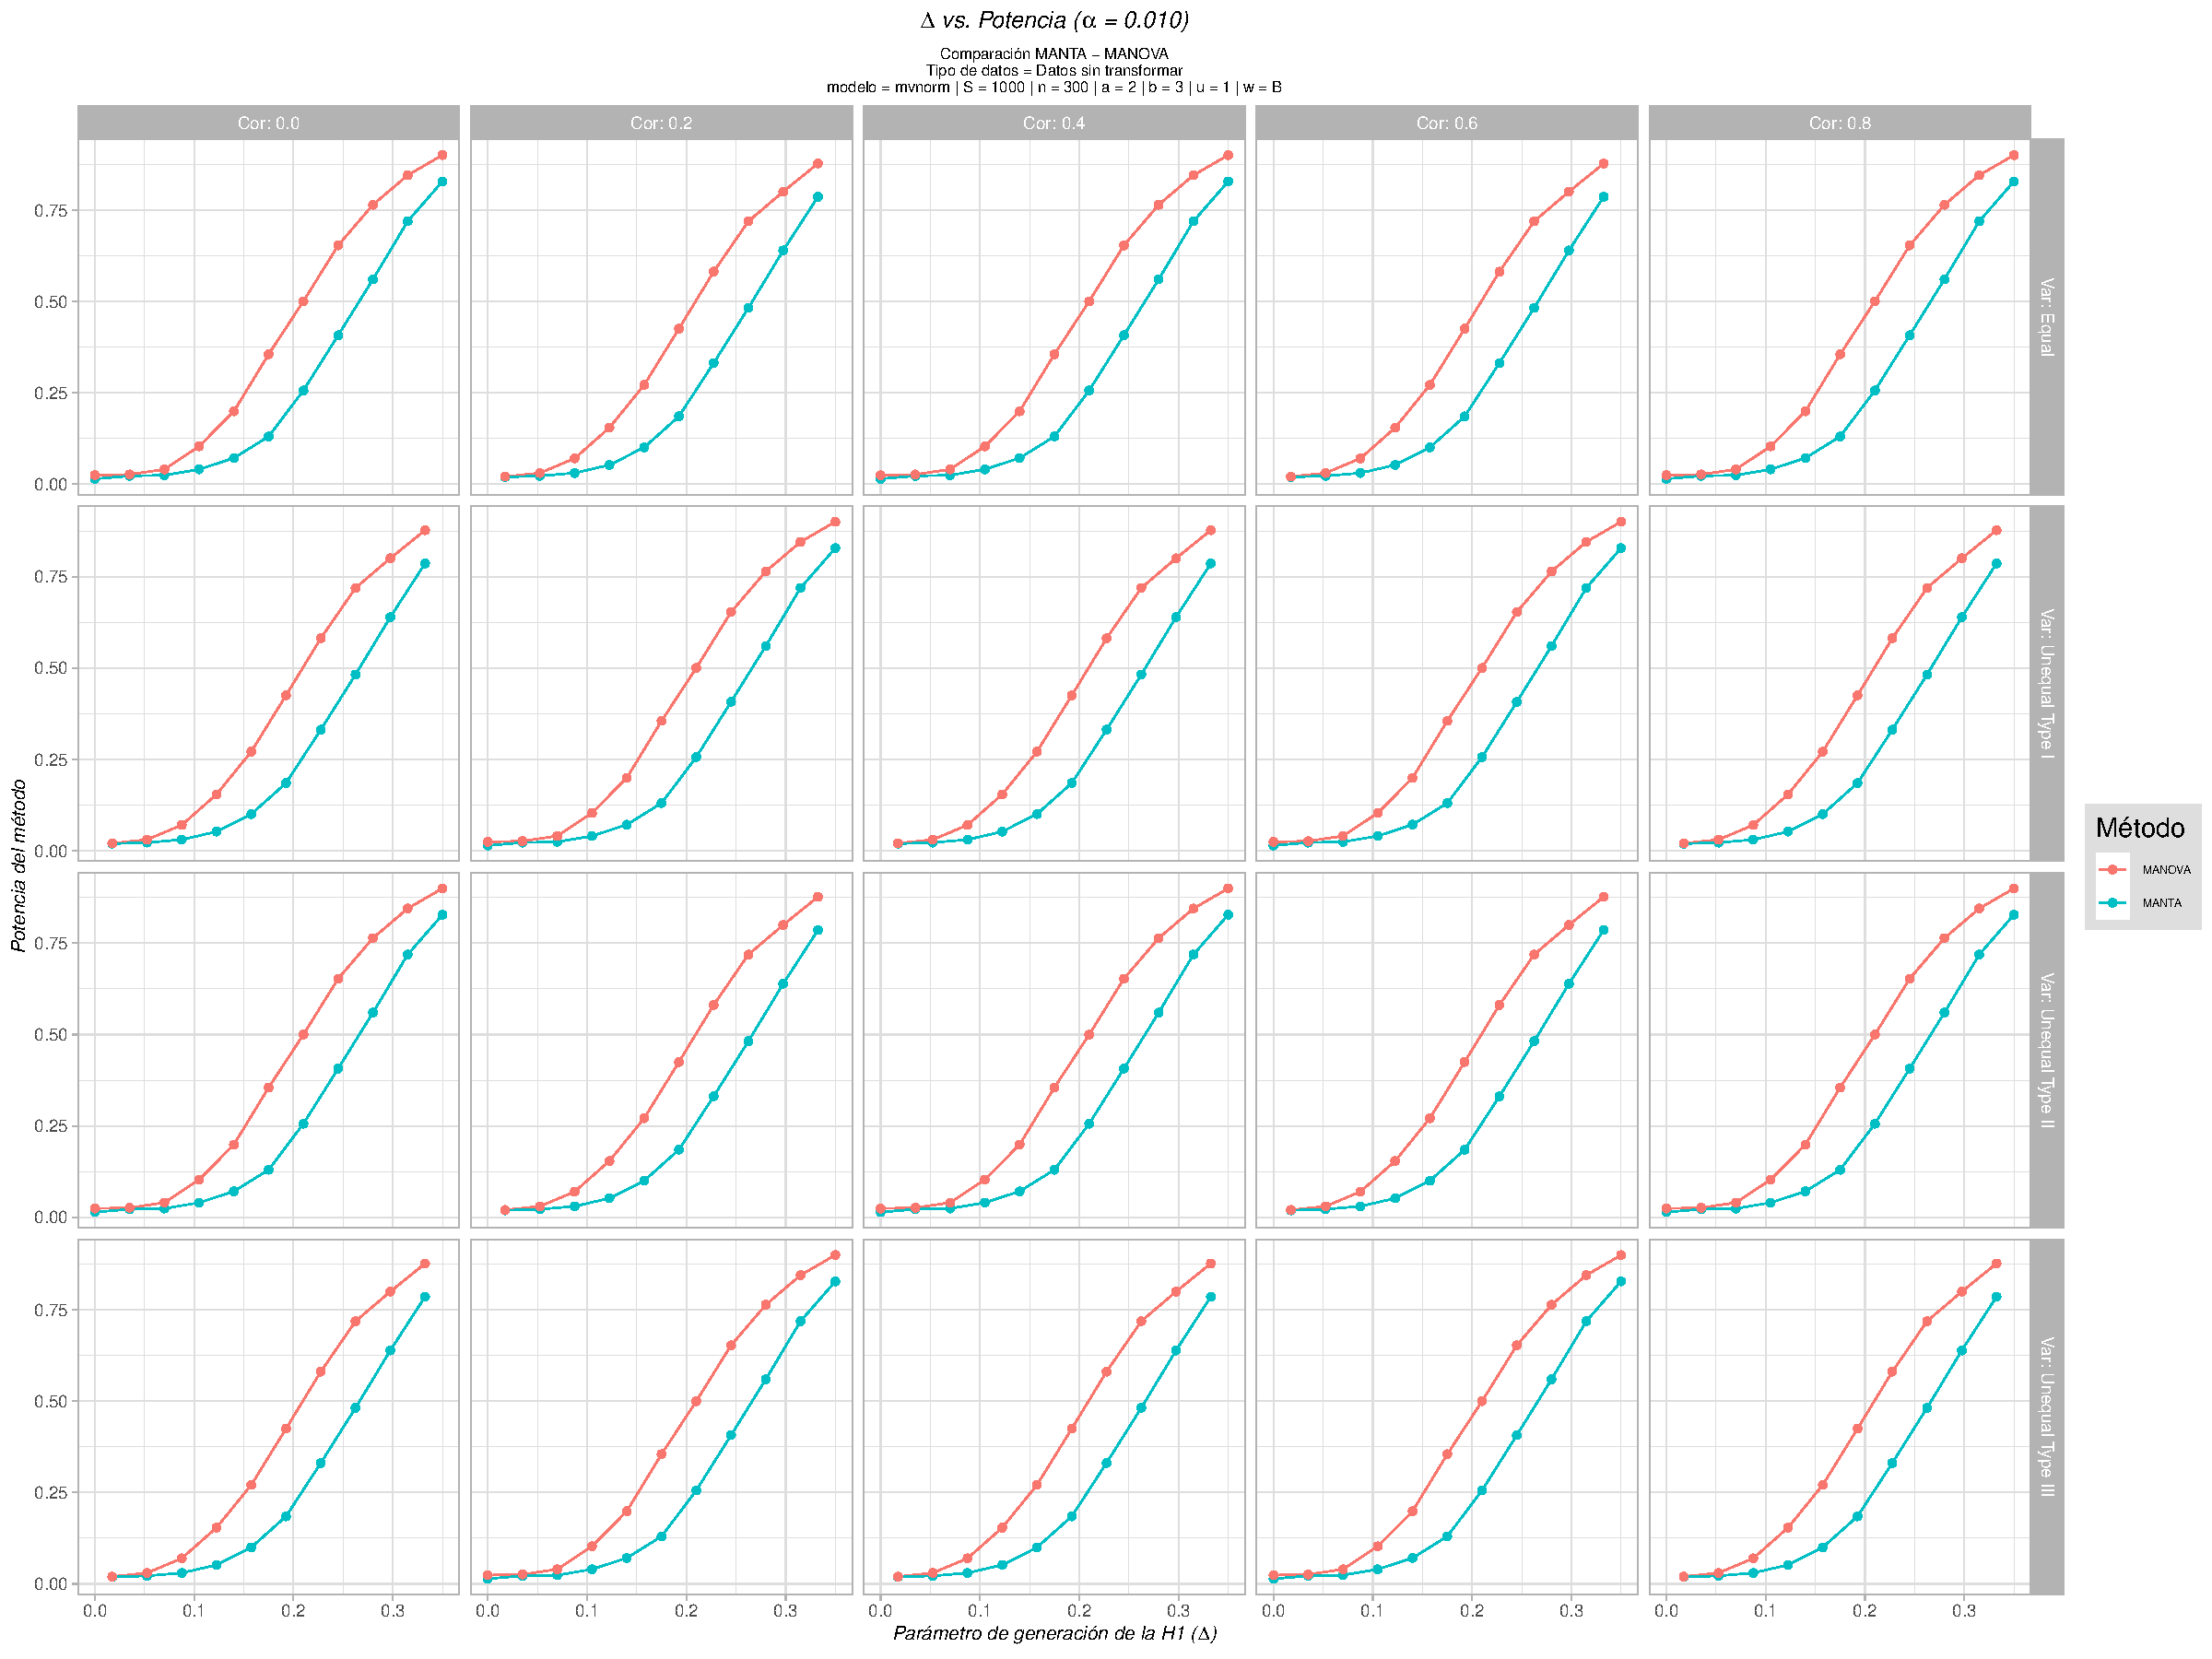
\includegraphics[width=.9\linewidth]{OBJ1c2001.pdf}
  \caption{\scriptsize{A.}}
  \label{fig:OBJ1c2001}
\end{subfigure}%
\\
\\
\begin{subfigure}{.65\textwidth}
\hspace*{3.5cm} % Movimiento relativo del gráfico
  \centering
  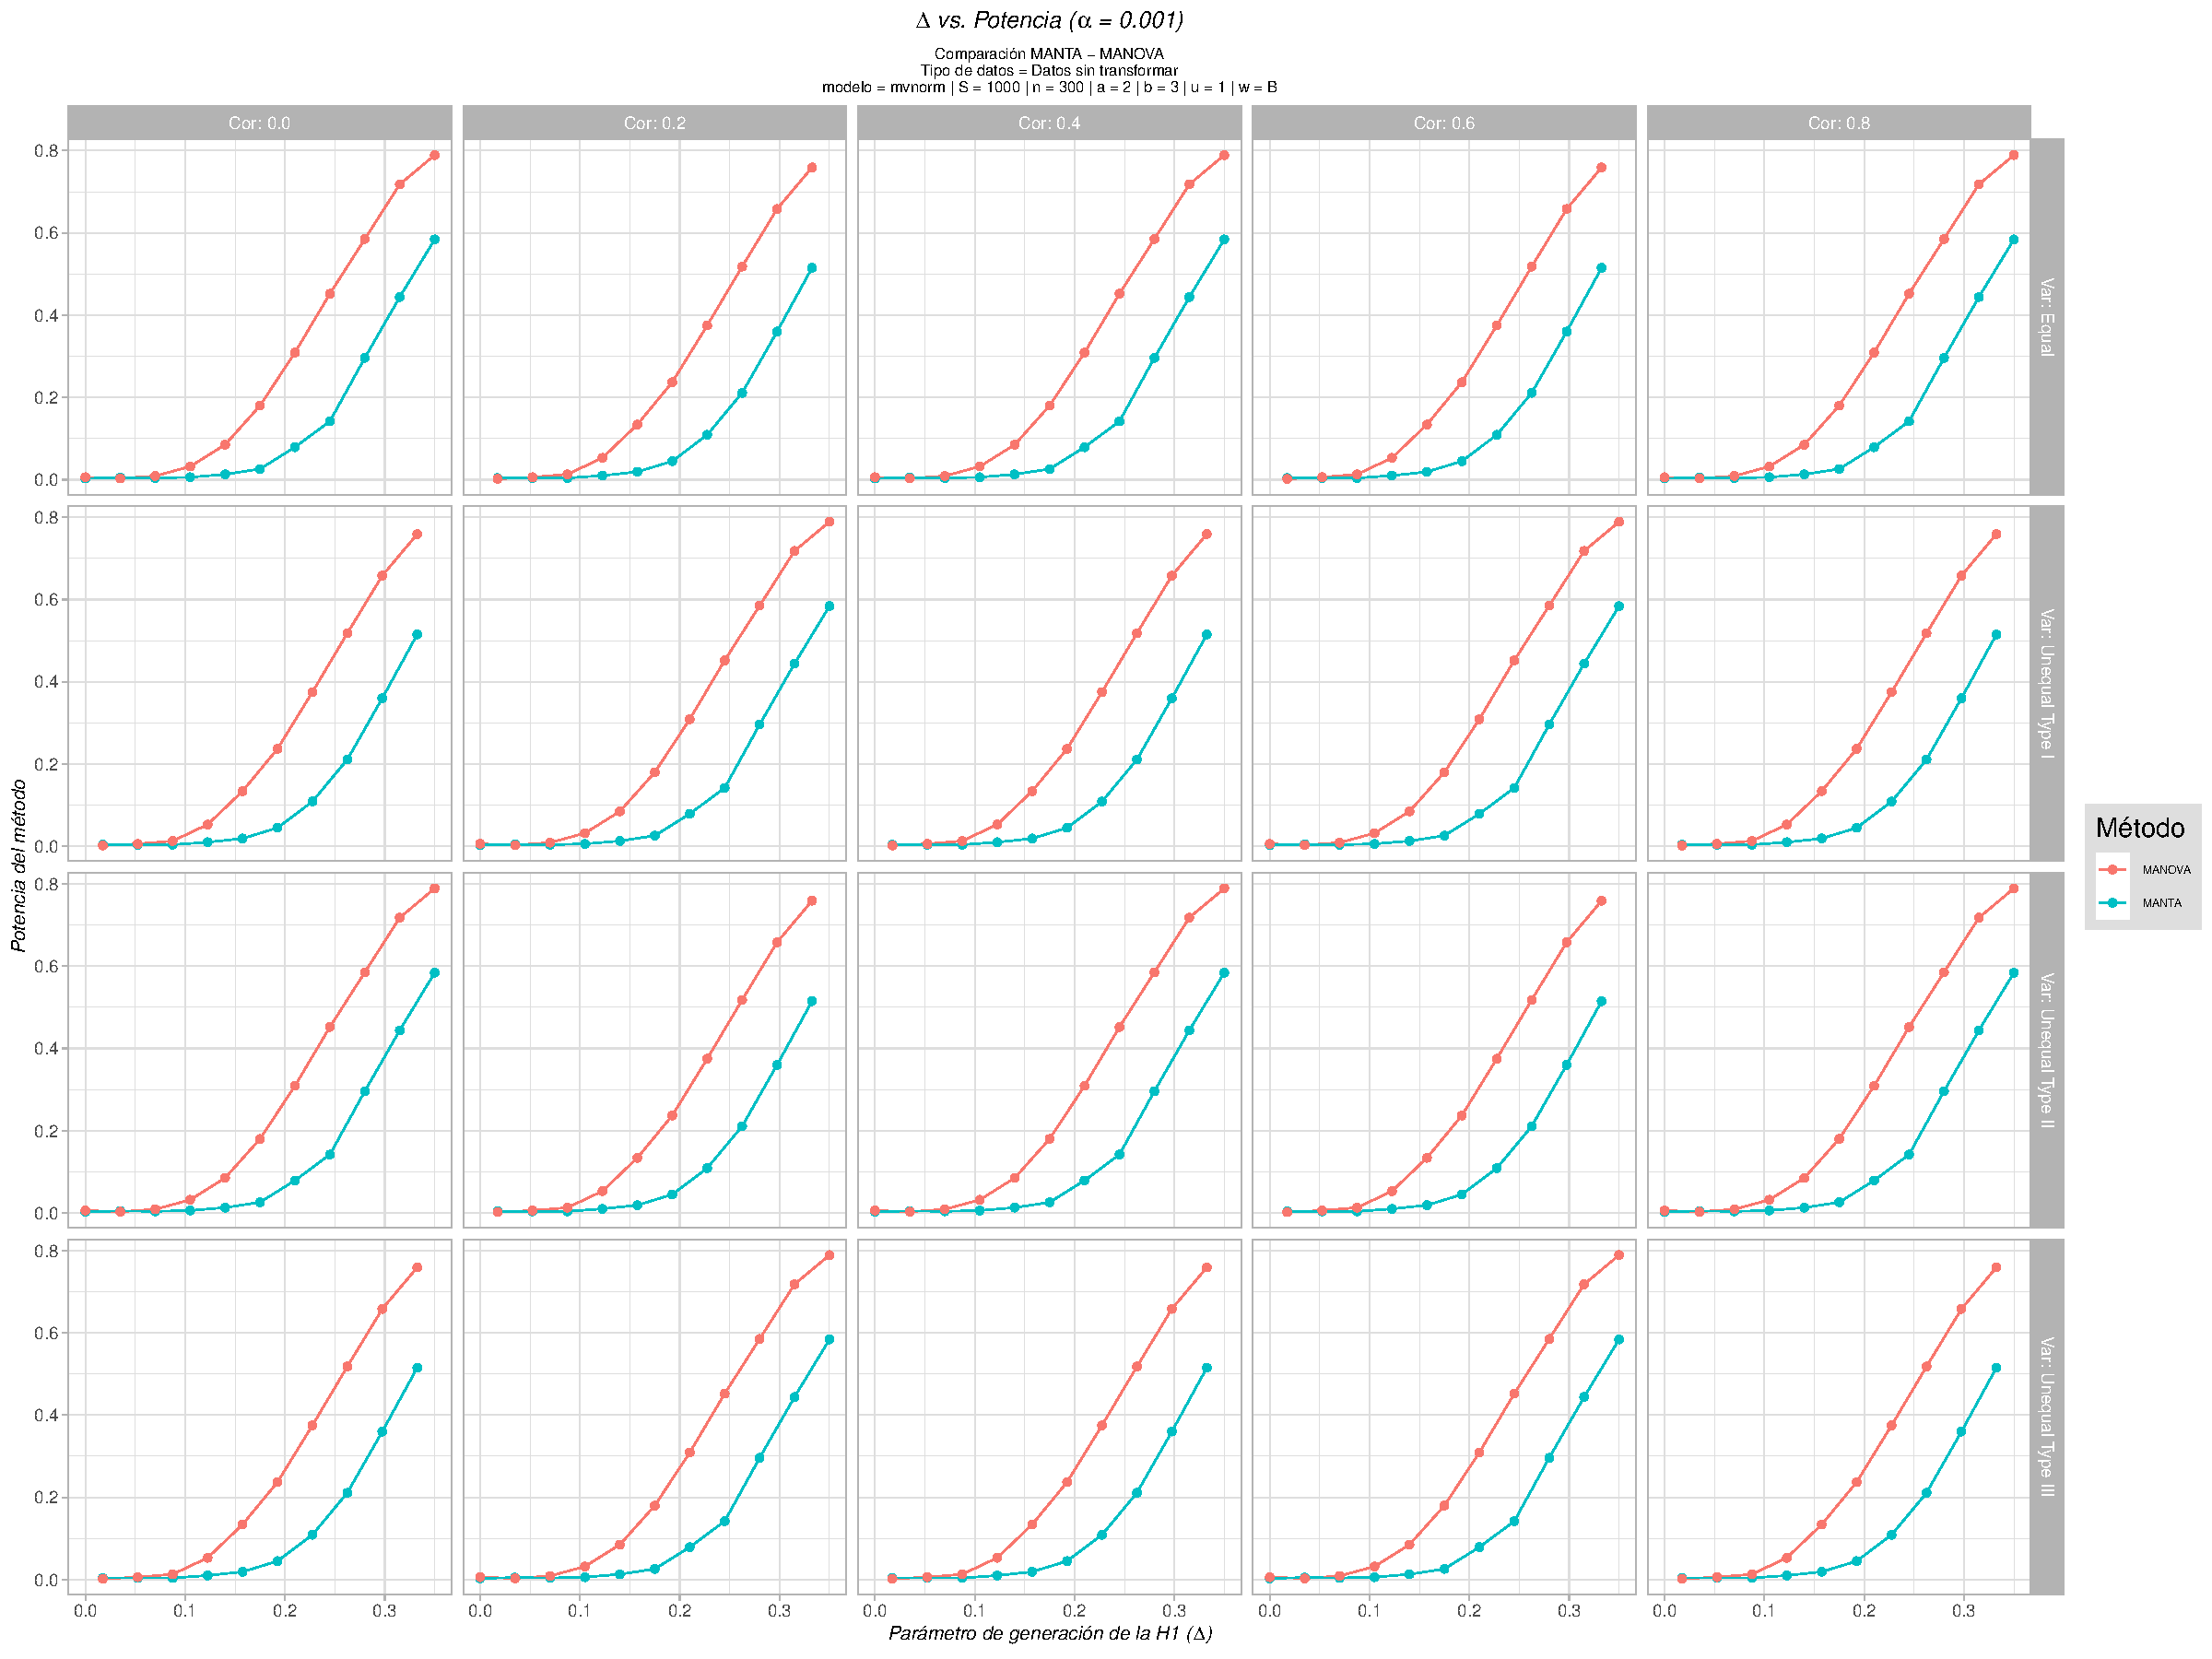
\includegraphics[width=.9\linewidth]{OBJ1c30001.pdf}
  \caption{\scriptsize{A.}}
  \label{fig:OBJ1c30001}
\end{subfigure}
\caption{\scriptsize{A.}}
\label{fig:OBJ1c}
\end{figure}

Finalmente, para concluir la exposición de los resultados obtenidos para los escenarios de simulación expuestos en el detallado del primer objetivo del presente trabajo, se añadirá del punto \textit{b} del primer objetivo:

% OBJ1dallalpha.pdf
\begin{figure}[!htbp]
\hspace*{-1.6cm} % Movimiento relativo del gráfico
    \centering
    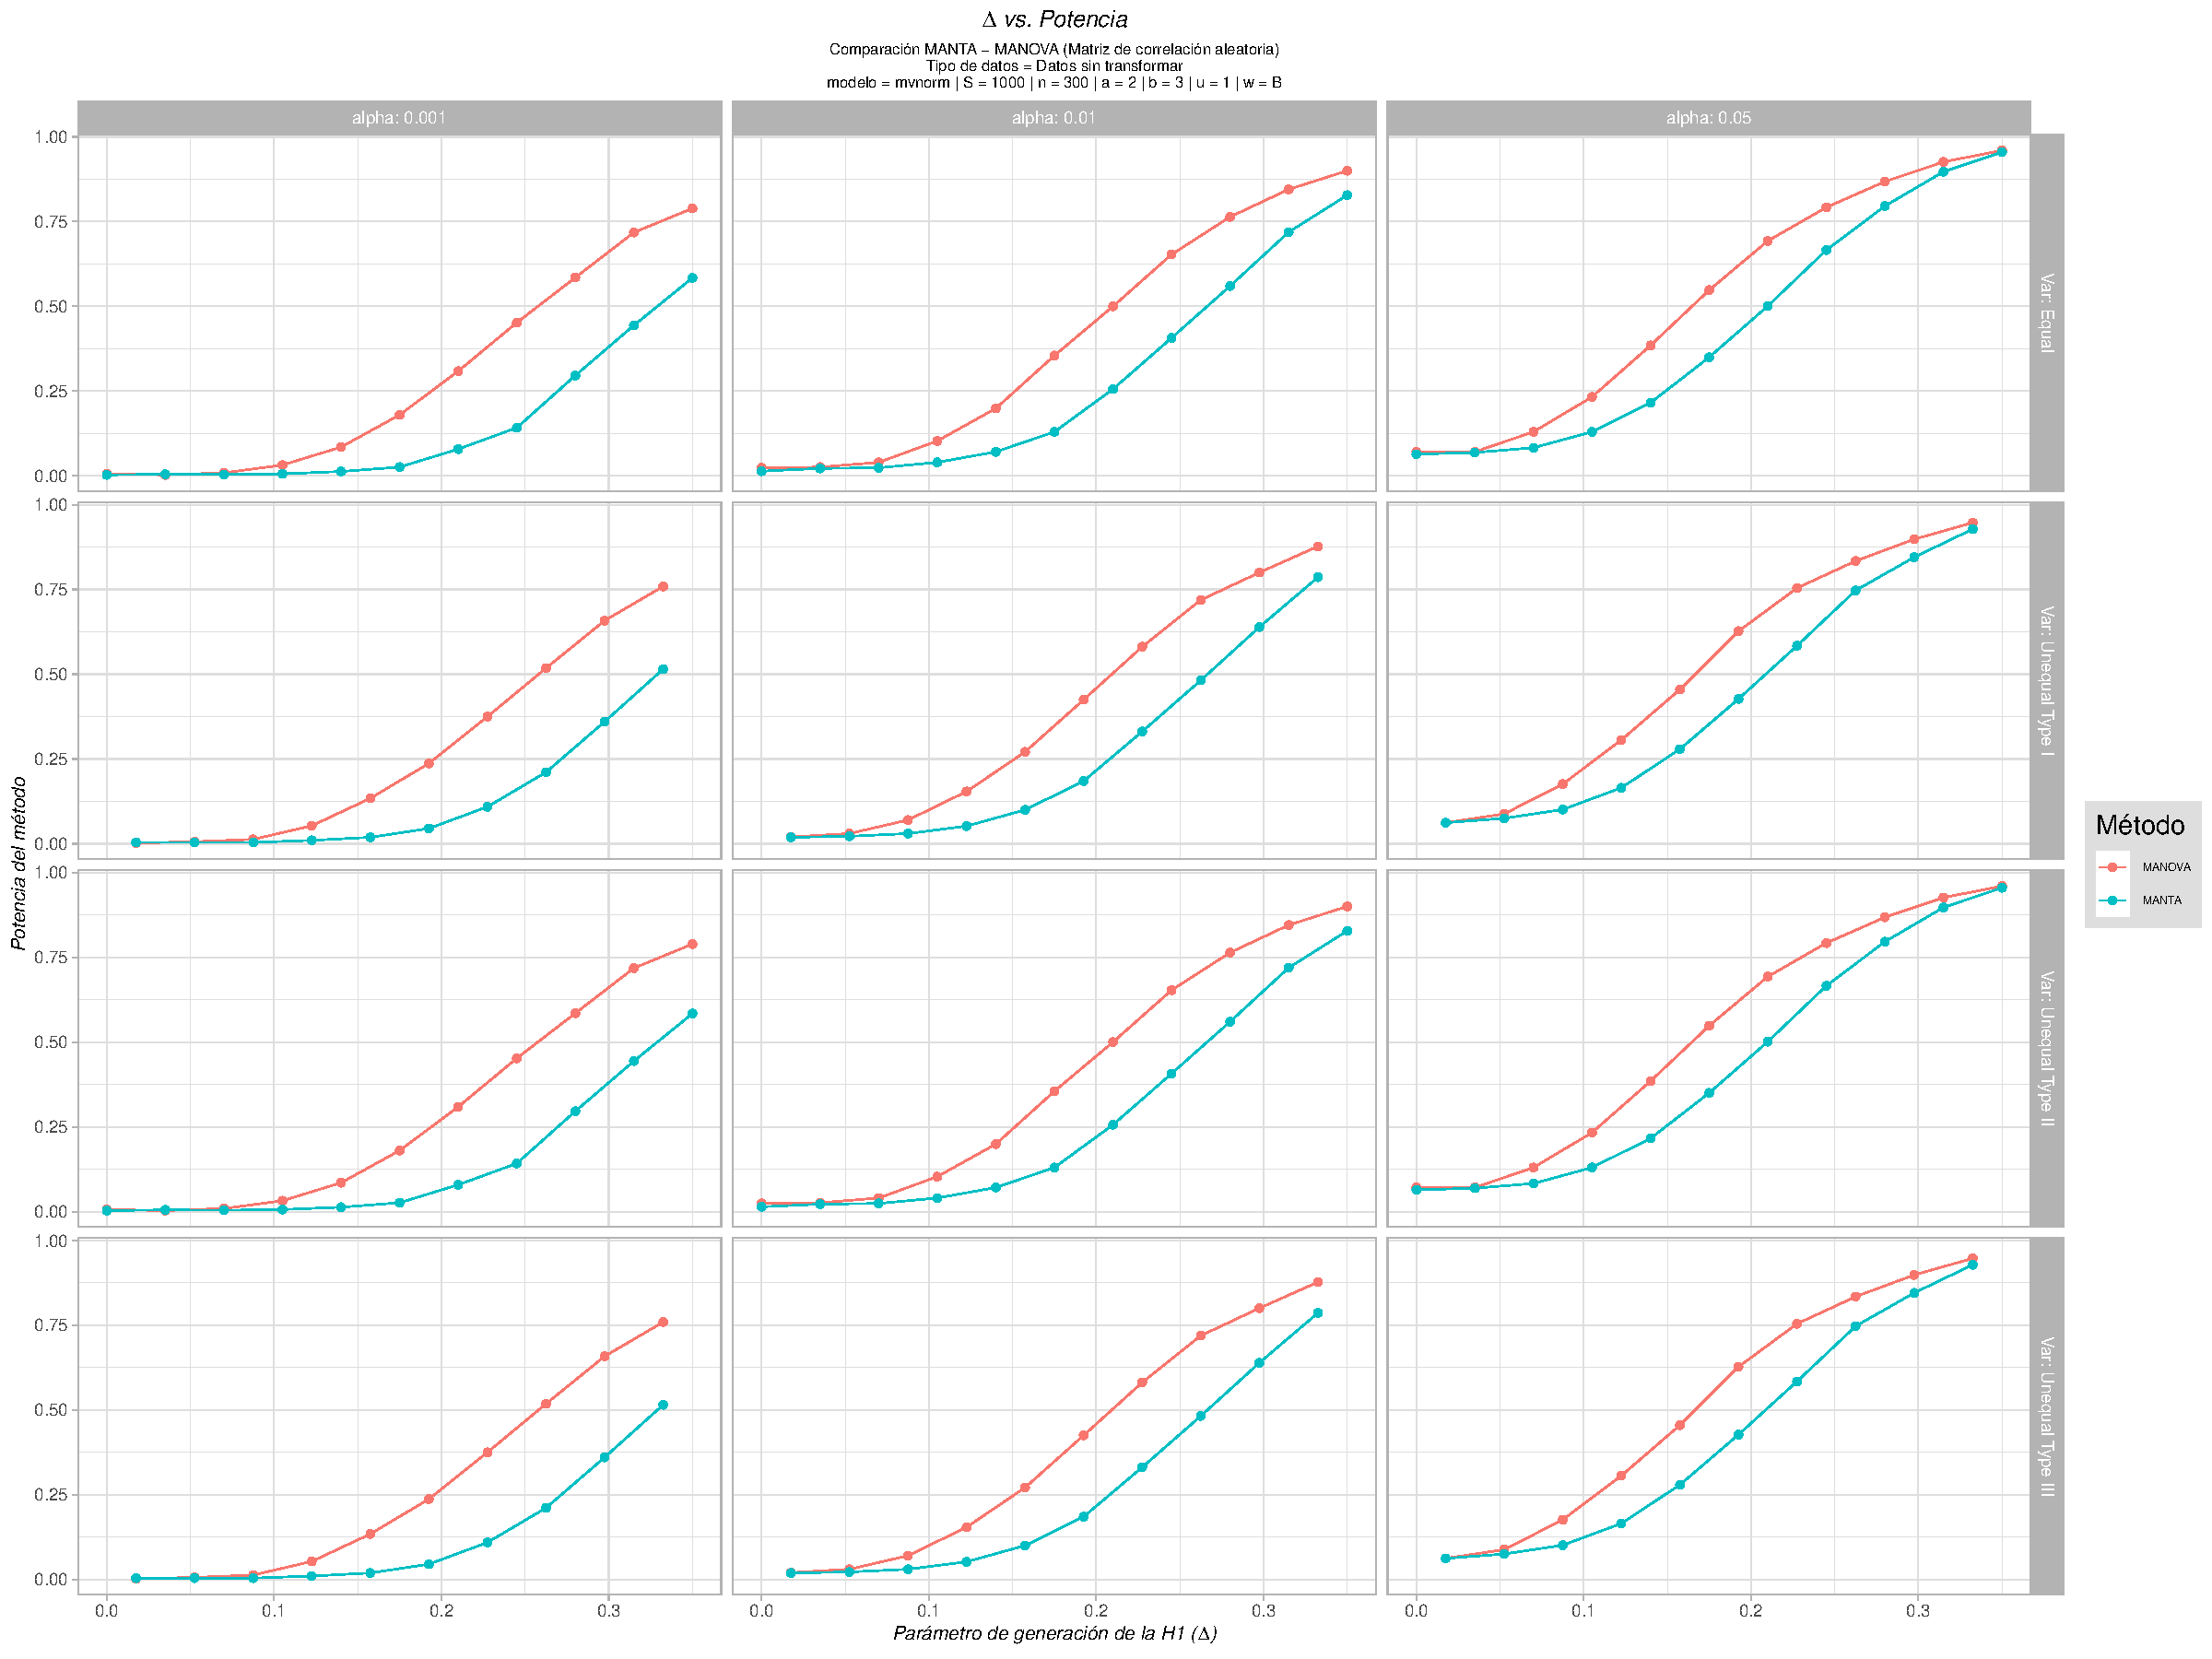
\includegraphics[scale=.51]{OBJ1dallalpha.pdf}
    \caption{\scriptsize{A.}}
    \label{fig:OBJ1dallalpha}
\end{figure}


\newpage
\subsection{Resultados del segundo objetivo}
\label{sec:Resultados del segundo objetivo}

En esta subsección se detallarán los resultados del segundo objetivo procediendo, como en el caso anterior, a mostrar en forma de malla gráfica comparativa los diversos supuestos de simulación. 

\

Previamente, se mostrará a modo de ejemplo una tabla con valores aleatorios del conjunto de datos generado tras la computación del escenario expuesto en \ref{TabSim02010156Sim09011559a} y \ref{TabSim02010156Sim09011559b}, el cual contiene información sobre el valor de las variables involucradas en cada una de las simulaciones, así como el valor del cálculo de la potencia estadística correspondiente, y el tiempo empleado:

% Tabla con ejemplos aleatorios de las simulaciones simplex:
\begin{table}[!htbp] \centering 
  \caption{\scriptsize{Muestra aleatoria de 15 de los 2144 resultados obtenidos para los 
   cálculos de la potencia estadística \( \mathbb P \) bajo las condiciones detalladas en  
   las simulaciones \ref{TabSim02010156Sim09011559a} y \ref{TabSim02010156Sim09011559b}.}} 
  \label{tab:AleatHeadSim02010156Sim09011559} 
\scriptsize 
\begin{tabular}{@{\extracolsep{-8pt}} cccccccccccc} 
\\ \specialrule{.1em}{.05em}{.05em} 
\specialrule{.1em}{.05em}{.05em} 
Datos & Modelo & alpha & S & n & Var & q & Cor & delta & Método & Potencia & t comp.\( (s) \) \\ 
\specialrule{.1em}{.05em}{.05em} 
Transformación raíz cuadrada & simplex & 0.0500 & 1,000 & 300 & 5 & 3 & 0.0260 & 0.0250 & MANTA & 1 & 13.1700 \\ 
Transformación raíz cuadrada & simplex & 0.0100 & 1,000 & 300 & 5 & 1 & 0.0270 & 0.0235 & MANTA & 1 & 10.4600 \\ 
Datos sin transformar & simplex & 0.0500 & 1,000 & 300 & 3 & 5 & 0.0230 & 0.0005 & MANTA & 0.0480 & 1.1400 \\ 
Transformación raíz cuadrada & simplex & 0.0500 & 1,000 & 300 & 3 & 3 & 0.0240 & 0.0240 & MANTA & 1 & 17.3500 \\ 
Datos sin transformar & simplex & 0.0500 & 1,000 & 300 & 5 & 3 & 0.0260 & 0.0090 & MANTA & 0.7960 & 1.1000 \\ 
Transformación logarítmica & simplex & 0.0500 & 1,000 & 300 & 5 & 3 & 0.0260 & 0.0170 & MANTA & 1 & 1 \\ 
Transformación Centered Log Ratio (clr) & simplex & 0.0010 & 1,000 & 300 & 3 & 5 & 0.0230 & 0.0085 & MANTA & 0.0900 & 1.0500 \\ 
Transformación raíz cuadrada & simplex & 0.0100 & 1,000 & 300 & 3 & 5 & 0.0230 & 0.0080 & MANTA & 0.5310 & 1.4400 \\ 
Transformación Centered Log Ratio (clr) & simplex & 0.0500 & 1,000 & 300 & 5 & 2 & 0.0270 & 0.0175 & MANTA & 0.9970 & 1.0500 \\ 
Datos sin transformar & simplex & 0.0010 & 1,000 & 300 & 3 & 3 & 0.0240 & 0.0140 & MANTA & 0.9710 & 1.0900 \\ 
Transformación logarítmica & simplex & 0.0010 & 1,000 & 300 & 3 & 5 & 0.0230 & 0.0045 & MANTA & 0.0260 & 0.9900 \\ 
Datos sin transformar & simplex & 0.0010 & 1,000 & 300 & 3 & 5 & 0.0230 & 0.0005 & MANTA & 0 & 1.0700 \\ 
Transformación logarítmica & simplex & 0.0100 & 1,000 & 300 & 3 & 2 & 0.0240 & 0.0220 & MANTA & 1 & 1 \\ 
Transformación raíz cuadrada & simplex & 0.0500 & 1,000 & 300 & 3 & 5 & 0.0230 & 0.0165 & MANTA & 1 & 14.2000 \\ 
Datos sin transformar & simplex & 0.0010 & 1,000 & 300 & 5 & 1 & 0.0270 & 0.0020 & MANTA & 0.0010 & 1.1300 \\ 
\specialrule{.1em}{.05em}{.05em} 
\end{tabular} 
\end{table}

Además, se han realizado un seguido de sumarios del estimador estadístico principal (\( \mathbb P \)), a la vez que del tiempo de computación (\textit{t comp.}), para los diferentes tipos de subgrupos de simulación definidos por las transformaciones de datos aplicadas, con el fin de poder aportar más información a la interpretación de los resultados que se mostrarán más adelante.

Para una mejor interpretación, se han realizado representaciones gráficas de estos estadísticos en forma de distribuciones de densidad, forzando la comparativa entre diversas variables para garantizar una correcta visualización de las posibles dependencias entre ellas (\ref{fig:OBJ2SimplexStatswrapAlpha} y \ref{fig:OBJ2SimplexStatsGridqloc}).

\newpage
% Sumarios estadísticos de la Potencia y el Tiempo de computación según el tipo de datos y alpha (símplex):
%% Datos sin transformar
\begin{table}[!htbp] \centering 
  \caption{\scriptsize{Sumario estadístico (para diferentes valores del nivel de significación \( \alpha \)) 
  de la potencia estadística (\( \mathbb P \)) calculada, y del tiempo de computación empleado en las 
  simulaciones \textit{3-símplex}, sin aplicar al conjunto de datos ninguna transformación.}}
  \label{tab:SummarySimplexNoTransfAllAlpha}
% \hspace*{-2cm} % Movimiento relativo del gráfico
\begin{subtable}[t]{0.48\textwidth}
\tiny
\centering
\begin{tabular}{@{\extracolsep{-8pt}}lccccc} 
\\ \specialrule{.1em}{.05em}{.05em} 
\specialrule{.1em}{.05em}{.05em} 
Statistic & \multicolumn{1}{c}{N} & \multicolumn{1}{c}{Mean} & \multicolumn{1}{c}{St. Dev.} & \multicolumn{1}{c}{Min} & \multicolumn{1}{c}{Max} \\ 
\specialrule{.1em}{.05em}{.05em} 
Potencia & 179 & 0.7593 & 0.3475 & 0.0470 & 1.0000 \\ 
tcomp & 179 & 1.1578 & 0.0798 & 1.0764 & 1.4821 \\ 
\specialrule{.1em}{.05em}{.05em} 
\end{tabular} 
\caption{Combinaciones \(\Delta - q - loc\): imponiendo un \( \alpha \in \text{0.05} \).}
\label{SummarySimplexNoTransf005}
\end{subtable}
\hfil
\begin{subtable}[t]{0.48\textwidth}
\tiny
\centering
\begin{tabular}{@{\extracolsep{-8pt}}lccccc} 
\\ \specialrule{.1em}{.05em}{.05em} 
\specialrule{.1em}{.05em}{.05em} 
Statistic & \multicolumn{1}{c}{N} & \multicolumn{1}{c}{Mean} & \multicolumn{1}{c}{St. Dev.} & \multicolumn{1}{c}{Min} & \multicolumn{1}{c}{Max} \\ 
\specialrule{.1em}{.05em}{.05em} 
Potencia & 178 & 0.6971 & 0.3906 & 0.0050 & 1.0000 \\ 
tcomp & 178 & 1.1214 & 0.0620 & 1.0489 & 1.3689 \\ 
\specialrule{.1em}{.05em}{.05em} 
\end{tabular} 
\caption{Combinaciones \(\Delta - q - loc\): imponiendo un \( \alpha \in \text{0.01} \).}
\label{SummarySimplexNoTransf001}
\end{subtable}
\hfil
\begin{subtable}[t]{0.48\textwidth}
\tiny
\centering
\begin{tabular}{@{\extracolsep{-8pt}}lccccc} 
\\ \specialrule{.1em}{.05em}{.05em} 
\specialrule{.1em}{.05em}{.05em} 
Statistic & \multicolumn{1}{c}{N} & \multicolumn{1}{c}{Mean} & \multicolumn{1}{c}{St. Dev.} & \multicolumn{1}{c}{Min} & \multicolumn{1}{c}{Max} \\ 
\specialrule{.1em}{.05em}{.05em} 
Potencia & 179 & 0.6277 & 0.4212 & 0.0000 & 1.0000 \\ 
tcomp & 179 & 1.1132 & 0.0546 & 1.0469 & 1.3755 \\ 
\specialrule{.1em}{.05em}{.05em}
\end{tabular}
\caption{Combinaciones \(\Delta - q - loc\): imponiendo un \( \alpha \in \text{0.001} \).}
\label{SummarySimplexNoTransf0001}
\end{subtable}
\end{table}


%% Transformación logarítmica
\begin{table}[!htbp] \centering 
  \caption{\scriptsize{Sumario estadístico (para diferentes valores del nivel de significación \( \alpha \)) 
  de la potencia estadística (\( \mathbb P \)) calculada, y el tiempo de computación empleado en las 
  simulaciones \textit{3-símplex}, aplicando al conjunto de datos una transformación logarítmica.}}
  \label{tab:SummarySimplexLogAllAlpha}
% \hspace*{-2cm} % Movimiento relativo del gráfico
\begin{subtable}[t]{0.48\textwidth}
\tiny
\centering
\begin{tabular}{@{\extracolsep{-8pt}}lccccc} 
\\ \specialrule{.1em}{.05em}{.05em} 
\specialrule{.1em}{.05em}{.05em} 
Statistic & \multicolumn{1}{c}{N} & \multicolumn{1}{c}{Mean} & \multicolumn{1}{c}{St. Dev.} & \multicolumn{1}{c}{Min} & \multicolumn{1}{c}{Max} \\ 
\specialrule{.1em}{.05em}{.05em} 
Potencia & 179 & 0.7516 & 0.3514 & 0.0470 & 1.0000 \\ 
tcomp & 179 & 1.0767 & 0.0917 & 0.9947 & 1.6458 \\ 
\specialrule{.1em}{.05em}{.05em} 
\end{tabular} 
\caption{Combinaciones \(\Delta - q - loc\): imponiendo un \( \alpha \in \text{0.05} \).}
\label{SummarySimplexLog005}
\end{subtable}
\hfil
\begin{subtable}[t]{0.48\textwidth}
\tiny
\centering
\begin{tabular}{@{\extracolsep{-8pt}}lccccc} 
\\ \specialrule{.1em}{.05em}{.05em} 
\specialrule{.1em}{.05em}{.05em} 
Statistic & \multicolumn{1}{c}{N} & \multicolumn{1}{c}{Mean} & \multicolumn{1}{c}{St. Dev.} & \multicolumn{1}{c}{Min} & \multicolumn{1}{c}{Max} \\ 
\specialrule{.1em}{.05em}{.05em} 
Potencia & 178 & 0.6878 & 0.3942 & 0.0060 & 1.0000 \\ 
tcomp & 178 & 1.0395 & 0.0462 & 0.9804 & 1.2416 \\ 
\specialrule{.1em}{.05em}{.05em} 
\end{tabular} 
\caption{Combinaciones \(\Delta - q - loc\): imponiendo un \( \alpha \in \text{0.01} \).}
\label{SummarySimplexLog001}
\end{subtable}
\hfil
\begin{subtable}[t]{0.48\textwidth}
\tiny
\centering
\begin{tabular}{@{\extracolsep{-8pt}}lccccc} 
\\ \specialrule{.1em}{.05em}{.05em} 
\specialrule{.1em}{.05em}{.05em} 
Statistic & \multicolumn{1}{c}{N} & \multicolumn{1}{c}{Mean} & \multicolumn{1}{c}{St. Dev.} & \multicolumn{1}{c}{Min} & \multicolumn{1}{c}{Max} \\ 
\specialrule{.1em}{.05em}{.05em} 
Potencia & 179 & 0.6176 & 0.4236 & 0.0000 & 1.0000 \\ 
tcomp & 179 & 1.0469 & 0.0558 & 0.9882 & 1.3023 \\  
\specialrule{.1em}{.05em}{.05em}
\end{tabular}
\caption{Combinaciones \(\Delta - q - loc\): imponiendo un \( \alpha \in \text{0.001} \).}
\label{SummarySimplexLog0001}
\end{subtable}
\end{table}


%% Transformación clr
\begin{table}[!htbp] \centering 
  \caption{\scriptsize{Sumario estadístico (para diferentes valores del nivel de significación \( \alpha \)) 
  de la potencia estadística (\( \mathbb P \)) calculada, y el tiempo de computación empleado en las 
  simulaciones \textit{3-símplex}, aplicando al conjunto de datos una transformación \textit{Centered Log 
  Ratio} (\textit{clr}).}}
  \label{tab:SummarySimplexclrAllAlpha}
% \hspace*{-2cm} % Movimiento relativo del gráfico
\begin{subtable}[t]{0.48\textwidth}
\tiny
\centering
\begin{tabular}{@{\extracolsep{-8pt}}lccccc} 
\\ \specialrule{.1em}{.05em}{.05em} 
\specialrule{.1em}{.05em}{.05em} 
Statistic & \multicolumn{1}{c}{N} & \multicolumn{1}{c}{Mean} & \multicolumn{1}{c}{St. Dev.} & \multicolumn{1}{c}{Min} & \multicolumn{1}{c}{Max} \\ 
\specialrule{.1em}{.05em}{.05em} 
Potencia & 179 & 0.6964 & 0.3745 & 0.0510 & 1.0000 \\ 
tcomp & 179 & 1.1206 & 0.0843 & 1.0358 & 1.5834 \\ 
\specialrule{.1em}{.05em}{.05em} 
\end{tabular} 
\caption{Combinaciones \(\Delta - q - loc\): imponiendo un \( \alpha \in \text{0.05} \).}
\label{SummarySimplexclr005}
\end{subtable}
\hfil
\begin{subtable}[t]{0.48\textwidth}
\tiny
\centering
\begin{tabular}{@{\extracolsep{-8pt}}lccccc} 
\\ \specialrule{.1em}{.05em}{.05em} 
\specialrule{.1em}{.05em}{.05em} 
Statistic & \multicolumn{1}{c}{N} & \multicolumn{1}{c}{Mean} & \multicolumn{1}{c}{St. Dev.} & \multicolumn{1}{c}{Min} & \multicolumn{1}{c}{Max} \\ 
\specialrule{.1em}{.05em}{.05em} 
Potencia & 178 & 0.6112 & 0.4158 & 0.0050 & 1.0000 \\ 
tcomp & 178 & 1.0879 & 0.0470 & 1.0276 & 1.2818 \\ 
\specialrule{.1em}{.05em}{.05em} 
\end{tabular} 
\caption{Combinaciones \(\Delta - q - loc\): imponiendo un \( \alpha \in \text{0.01} \).}
\label{SummarySimplexclr001}
\end{subtable}
\hfil
\begin{subtable}[t]{0.48\textwidth}
\tiny
\centering
\begin{tabular}{@{\extracolsep{-8pt}}lccccc} 
\\ \specialrule{.1em}{.05em}{.05em} 
\specialrule{.1em}{.05em}{.05em} 
Statistic & \multicolumn{1}{c}{N} & \multicolumn{1}{c}{Mean} & \multicolumn{1}{c}{St. Dev.} & \multicolumn{1}{c}{Min} & \multicolumn{1}{c}{Max} \\ 
\specialrule{.1em}{.05em}{.05em} 
Potencia & 179 & 0.5194 & 0.4351 & 0.0000 & 1.0000 \\ 
tcomp & 179 & 1.0762 & 0.0375 & 1.0300 & 1.2588 \\   
\specialrule{.1em}{.05em}{.05em}
\end{tabular}
\caption{Combinaciones \(\Delta - q - loc\): imponiendo un \( \alpha \in \text{0.001} \).}
\label{SummarySimplexclr0001}
\end{subtable}
\end{table}


%% Transformación sqrt
\begin{table}[!htbp] \centering 
  \caption{\scriptsize{Sumario estadístico (para diferentes valores del nivel de significación \( \alpha \)) 
  de la potencia estadística (\( \mathbb P \)) calculada, y el tiempo de computación empleado en las 
  simulaciones \textit{3-símplex}, aplicando al conjunto de datos una transformación de \textit{raíz 
  cuadrada} (\textit{sqrt}).}}
  \label{tab:SummarySimplexsqrtAllAlpha}
% \hspace*{-2cm} % Movimiento relativo del gráfico
\begin{subtable}[t]{0.48\textwidth}
\tiny
\centering
\begin{tabular}{@{\extracolsep{-8pt}}lccccc} 
\\ \specialrule{.1em}{.05em}{.05em} 
\specialrule{.1em}{.05em}{.05em} 
Statistic & \multicolumn{1}{c}{N} & \multicolumn{1}{c}{Mean} & \multicolumn{1}{c}{St. Dev.} & \multicolumn{1}{c}{Min} & \multicolumn{1}{c}{Max} \\ 
\specialrule{.1em}{.05em}{.05em} 
Potencia & 179 & 0.7389 & 0.3574 & 0.0470 & 1.0000 \\ 
tcomp & 179 & 5.2245 & 12.1286 & 0.9998 & 95.8778 \\ 
\specialrule{.1em}{.05em}{.05em} 
\end{tabular} 
\caption{Combinaciones \(\Delta - q - loc\): imponiendo un \( \alpha \in \text{0.05} \).}
\label{SummarySimplexsqrt005}
\end{subtable}
\hfil
\begin{subtable}[t]{0.48\textwidth}
\tiny
\centering
\begin{tabular}{@{\extracolsep{-8pt}}lccccc} 
\\ \specialrule{.1em}{.05em}{.05em} 
\specialrule{.1em}{.05em}{.05em} 
Statistic & \multicolumn{1}{c}{N} & \multicolumn{1}{c}{Mean} & \multicolumn{1}{c}{St. Dev.} & \multicolumn{1}{c}{Min} & \multicolumn{1}{c}{Max} \\ 
\specialrule{.1em}{.05em}{.05em} 
Potencia & 178 & 0.6708 & 0.4002 & 0.0060 & 1.0000 \\ 
tcomp & 178 & 5.4130 & 13.1872 & 0.9952 & 101.6103 \\ 
\specialrule{.1em}{.05em}{.05em} 
\end{tabular} 
\caption{Combinaciones \(\Delta - q - loc\): imponiendo un \( \alpha \in \text{0.01} \).}
\label{SummarySimplexsqrt001}
\end{subtable}
\hfil
\begin{subtable}[t]{0.48\textwidth}
\tiny
\centering
\begin{tabular}{@{\extracolsep{-8pt}}lccccc} 
\\ \specialrule{.1em}{.05em}{.05em} 
\specialrule{.1em}{.05em}{.05em} 
Statistic & \multicolumn{1}{c}{N} & \multicolumn{1}{c}{Mean} & \multicolumn{1}{c}{St. Dev.} & \multicolumn{1}{c}{Min} & \multicolumn{1}{c}{Max} \\ 
\specialrule{.1em}{.05em}{.05em} 
Potencia & 179 & 0.5969 & 0.4278 & 0.0000 & 1.0000 \\ 
tcomp & 179 & 5.2086 & 12.1741 & 0.9893 & 96.1683 \\    
\specialrule{.1em}{.05em}{.05em}
\end{tabular}
\caption{Combinaciones \(\Delta - q - loc\): imponiendo un \( \alpha \in \text{0.001} \).}
\label{SummarySimplexsqrt0001}
\end{subtable}
\end{table}

\newpage

% Fig. OBJ2SimplexStatswrapAlpha.pdf + OBJ2SimplexStatsGridqloc.pdf
\begin{figure}
\centering
\begin{subfigure}{0.49\textwidth}
\centering
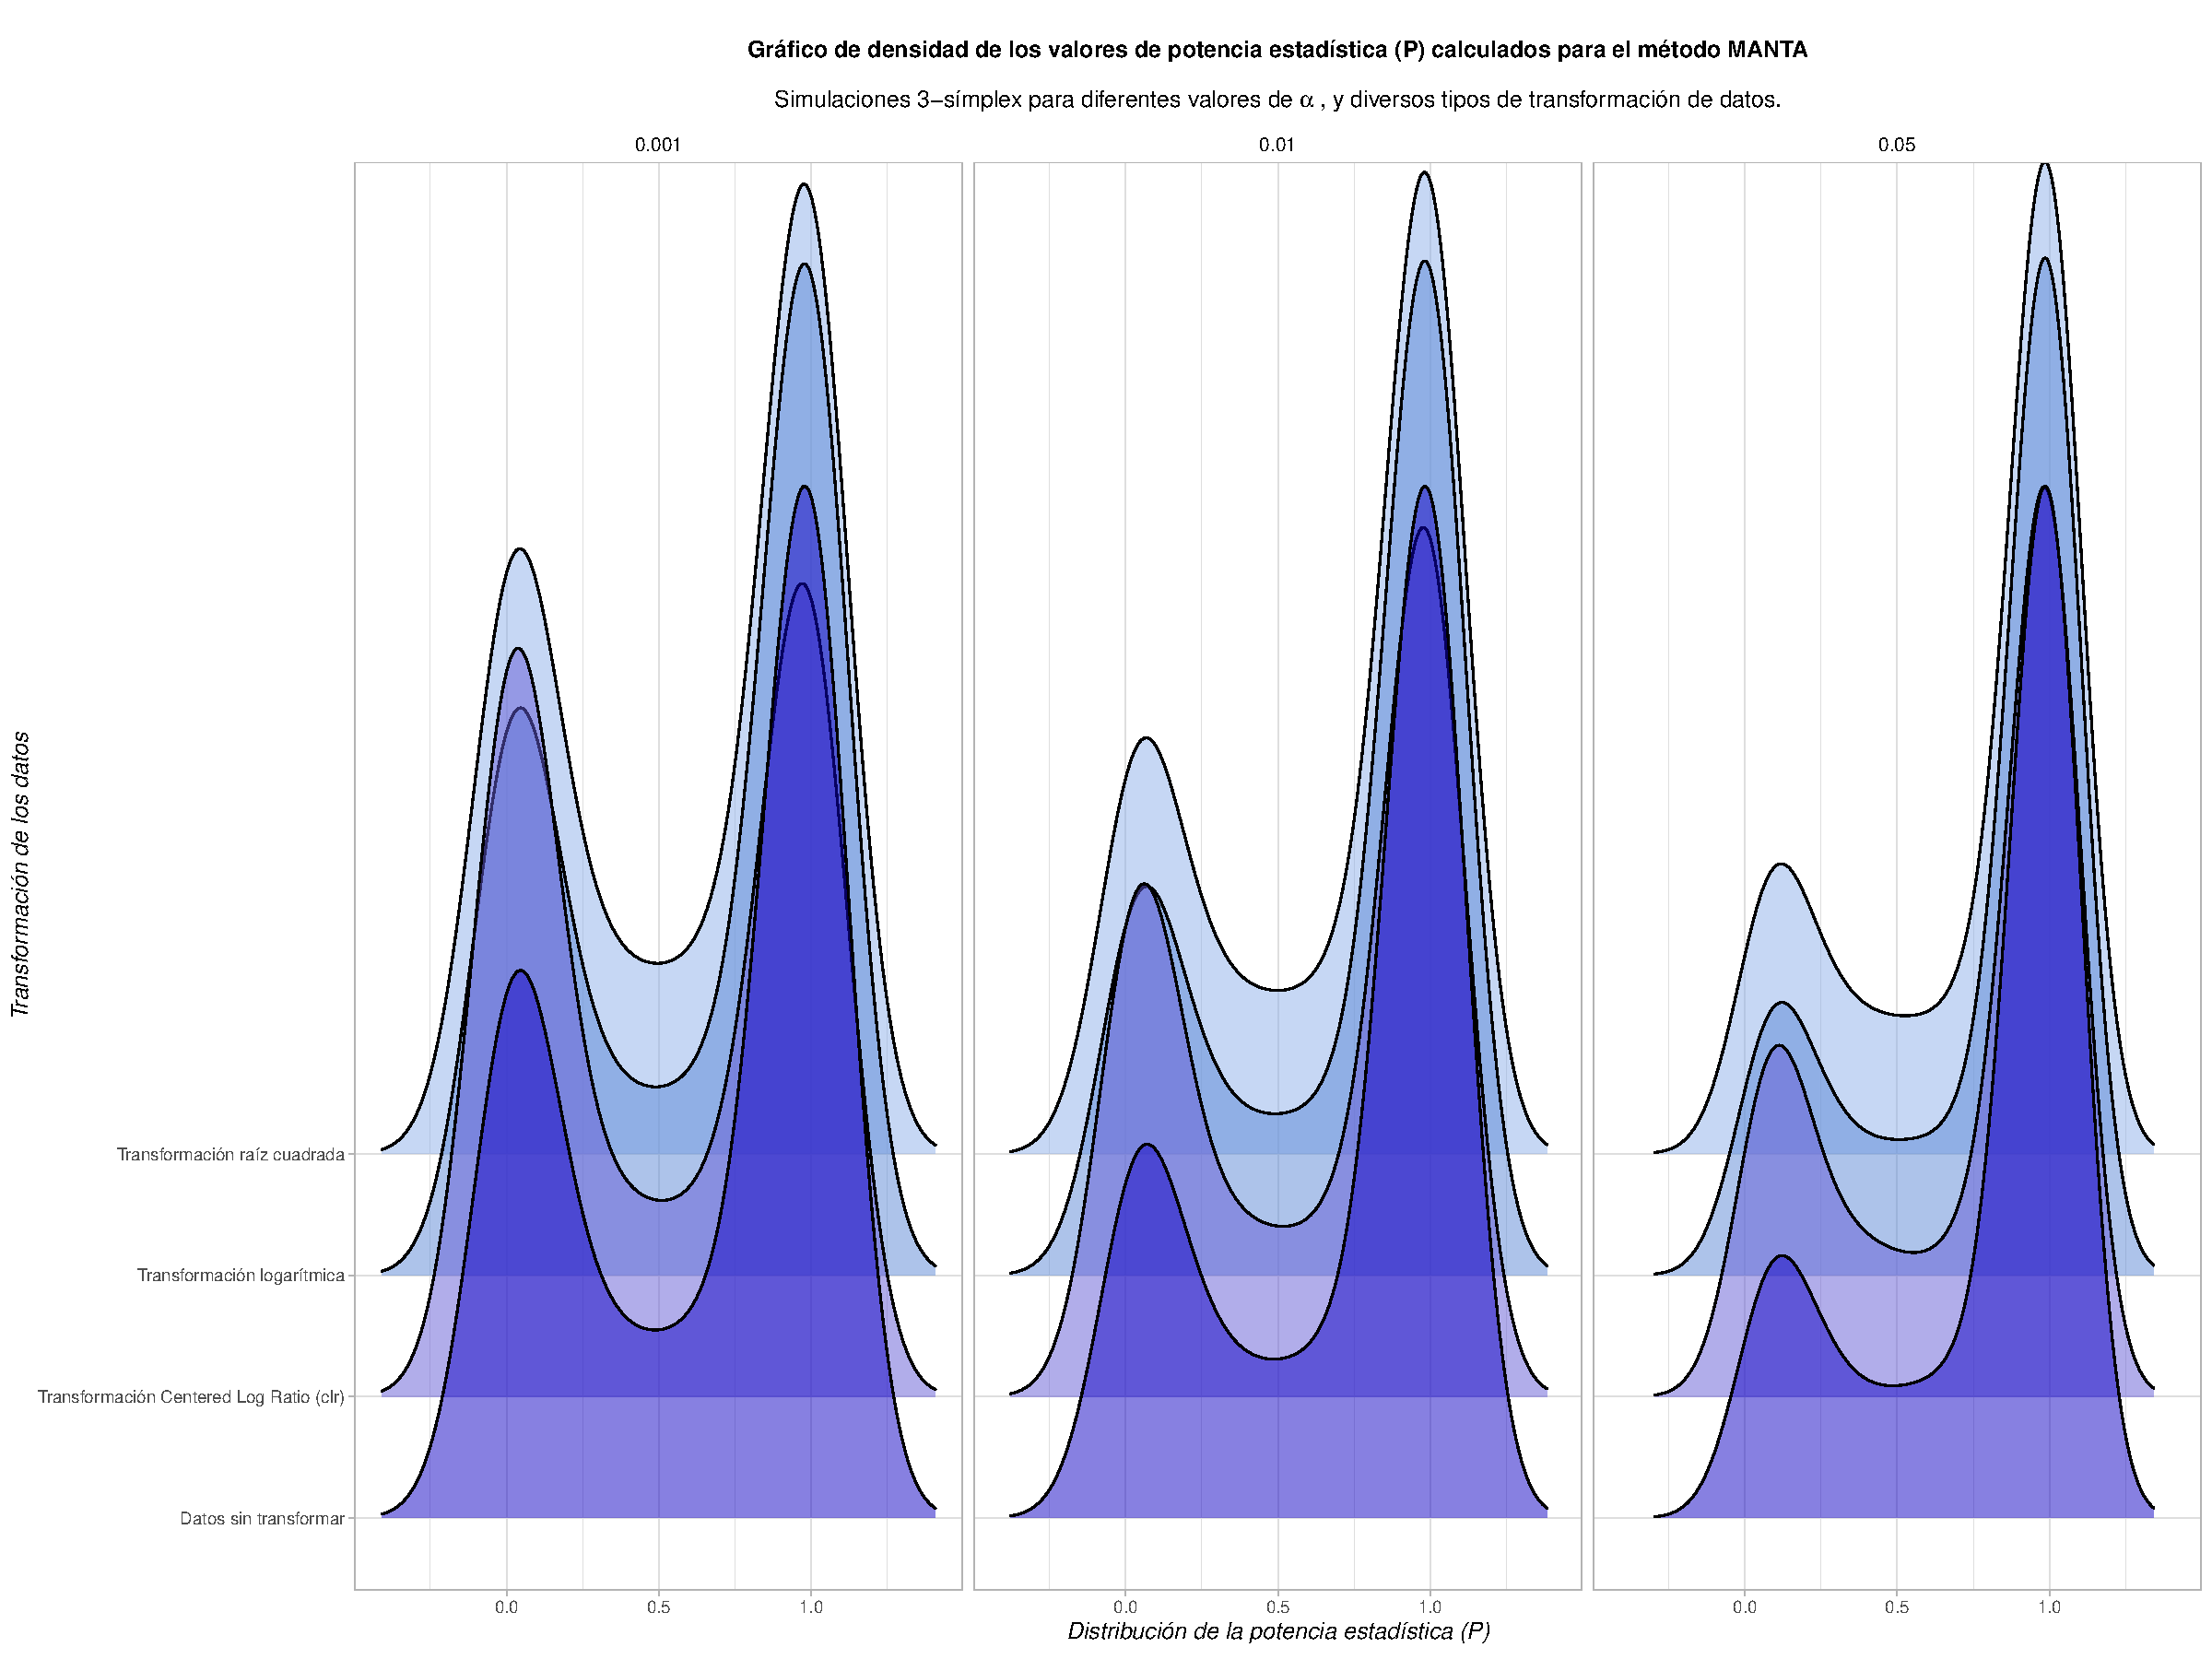
\includegraphics[width = \textwidth]{OBJ2SimplexStatswrapAlpha.pdf}
    \caption{\scriptsize{A.}}
    \label{fig:OBJ2SimplexStatswrapAlpha}
\end{subfigure}
\begin{subfigure}{0.49\textwidth}
\centering
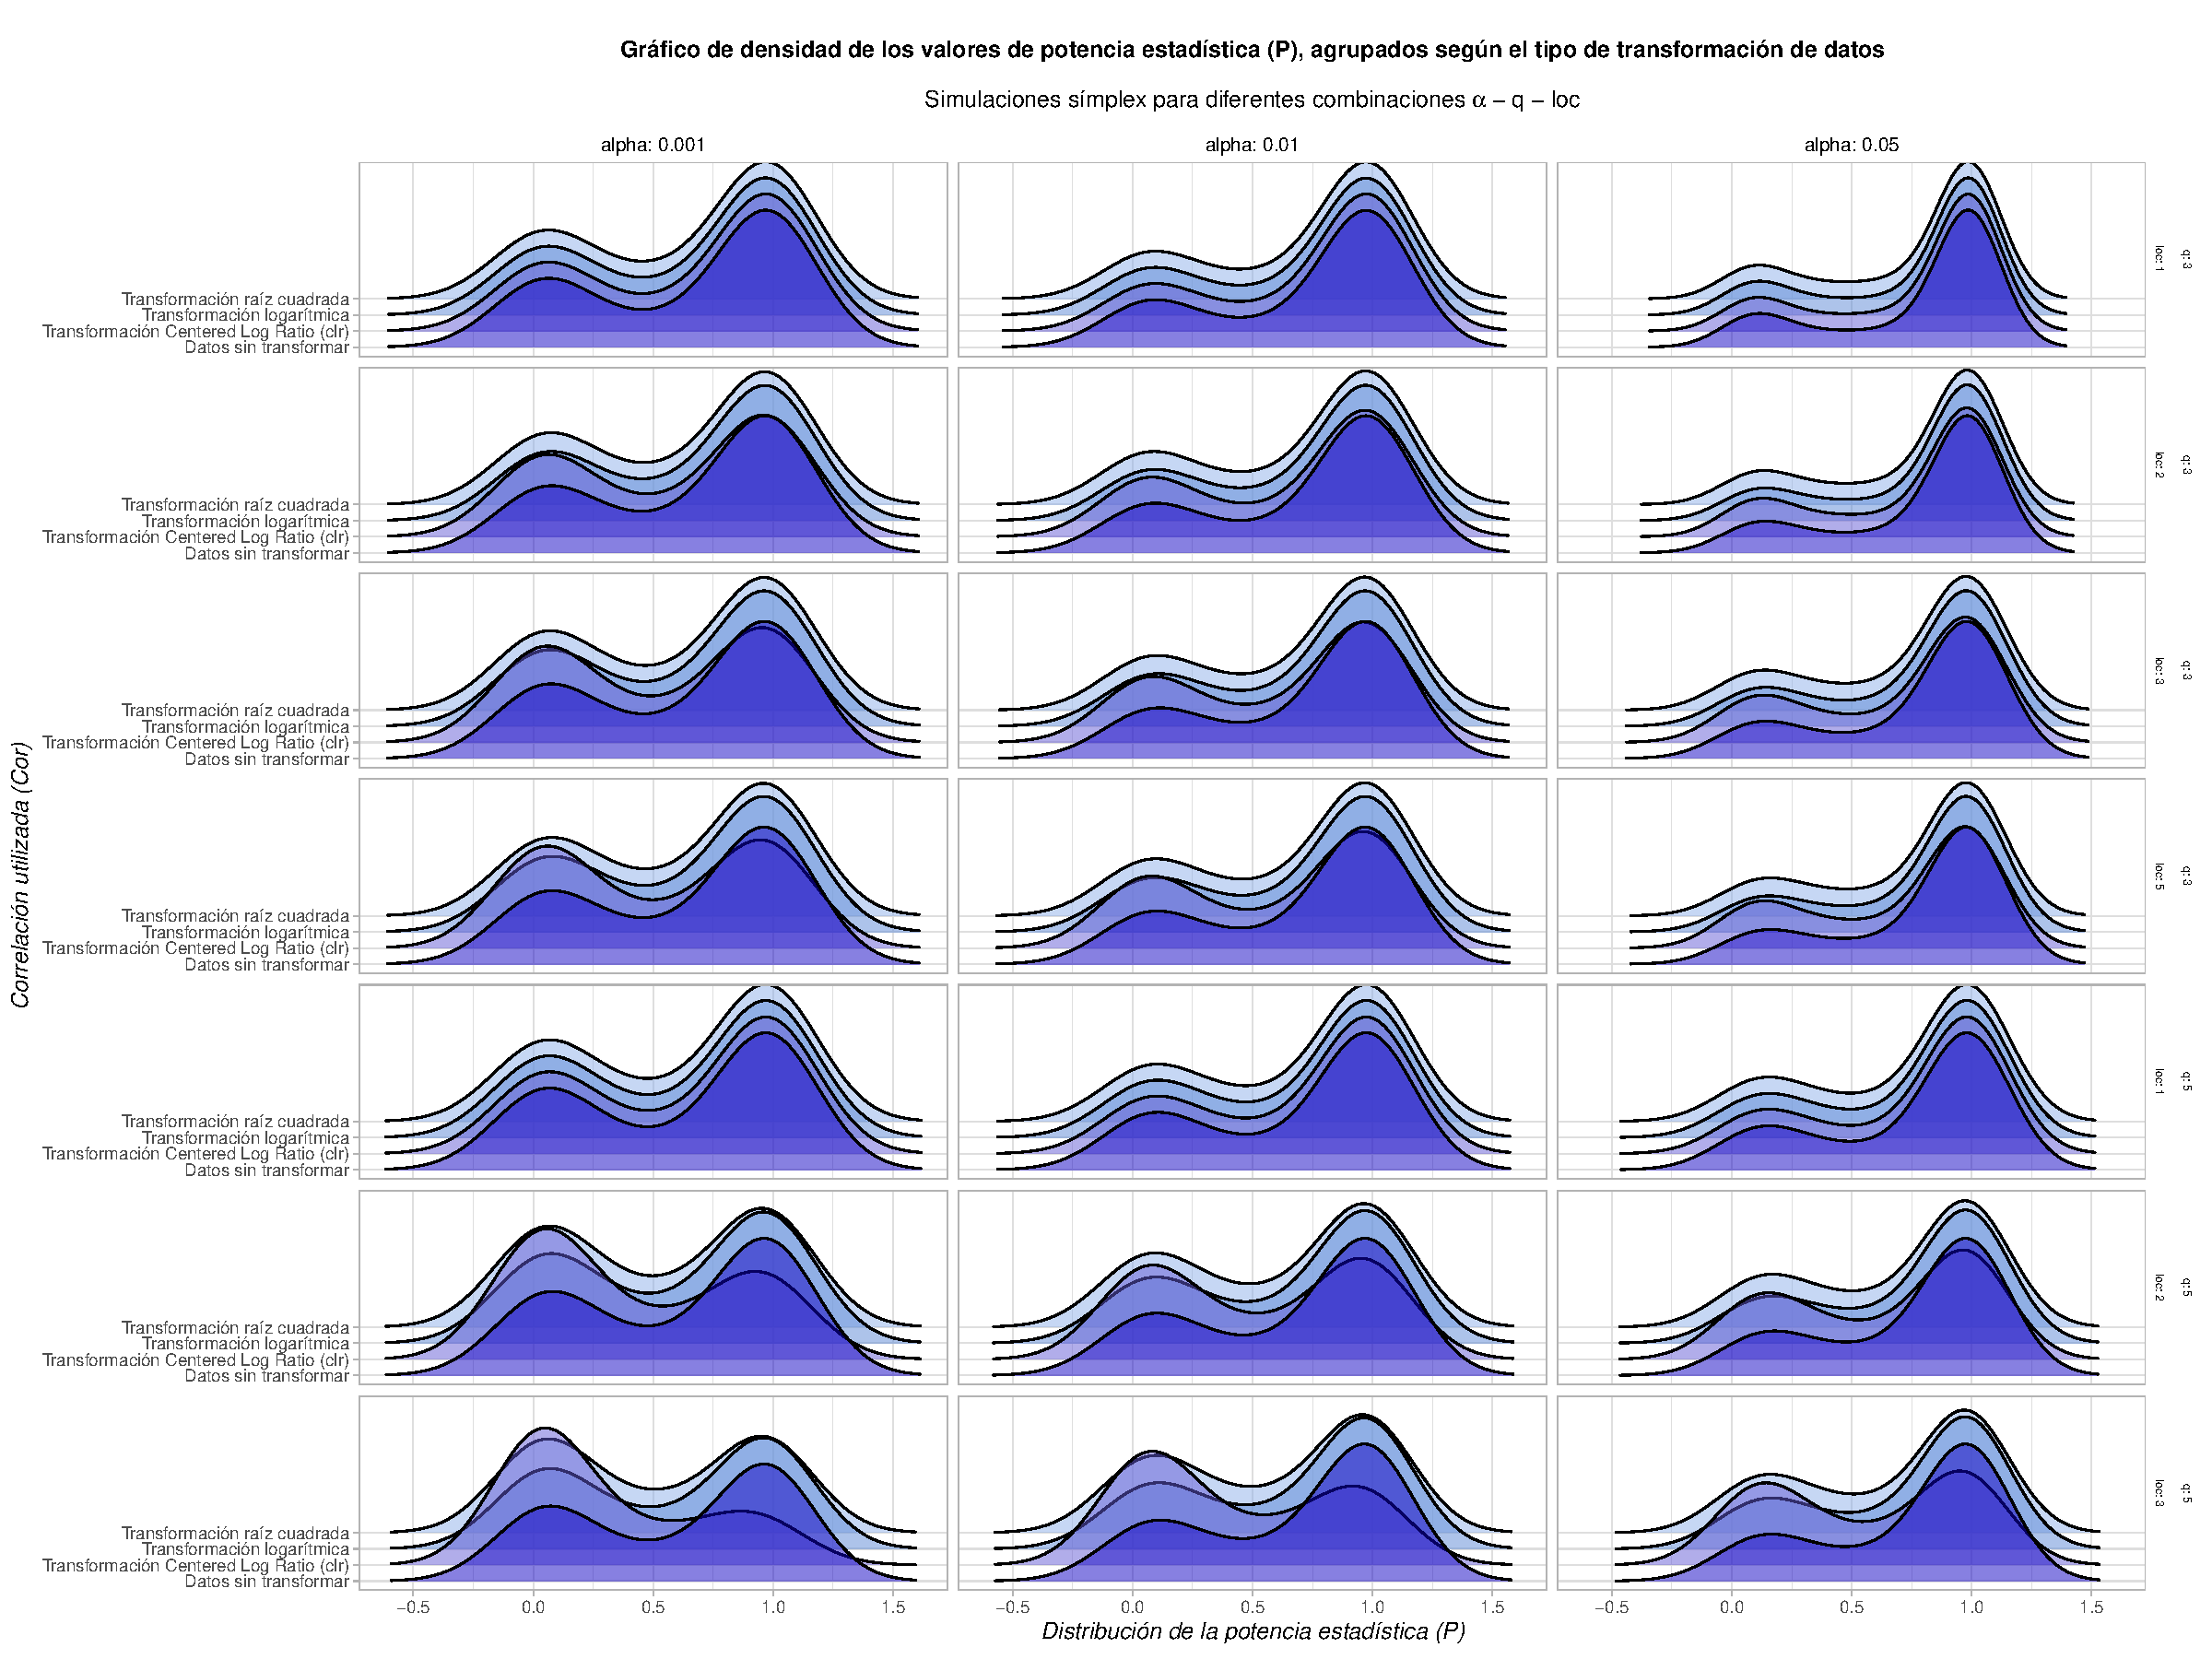
\includegraphics[width = \textwidth]{OBJ2SimplexStatsGridqloc.pdf}
    \caption{\scriptsize{A.}}
    \label{fig:OBJ2SimplexStatsGridqloc}
\end{subfigure}
\caption{OBJ1mvnormStatsHomog}
\label{fig:OBJ1mvnormStatsHomog}
\end{figure}

Tras lo anterior, y como primer resultado gráfico, se podrá encontrar el estudio de la posible invarianza frente a la transformación de los datos del método asintótico \textit{PERMANOVA} con respecto a su potencia estadística \( \mathbb P \) (calculada bajo un nivel de significación \( \alpha = \text{0.05} \)), teniendo en cuenta las siguientes variaciones \( \Delta - q - Loc \) en la simulación del conjunto de datos mediante el uso de un \textit{3-símplex}.

\

Para poder apreciar con más detalle la separación de los puntos de datos presentados en la figura \ref{fig:OBJ2SimplexMANTAqloc005}, se han realizado ampliaciones de las curvas agrandando las zonas pertenecientes a sendas colas: \textit{izquierda} (\textit{izqda.}) con valores bajos de \( \Delta \) (\ref{fig:OBJ2SimplexMANTAqloc005ColaIzq}), y la que muestra sus valores más altos (\textit{dcha.}) disponible en \ref{fig:OBJ2SimplexMANTAqloc005Coladch}.

% OBJ2SimplexMANTAqloc005.pdf
\begin{figure}[!htbp]
\hspace*{-0.8cm} % Movimiento relativo del gráfico
    \centering
    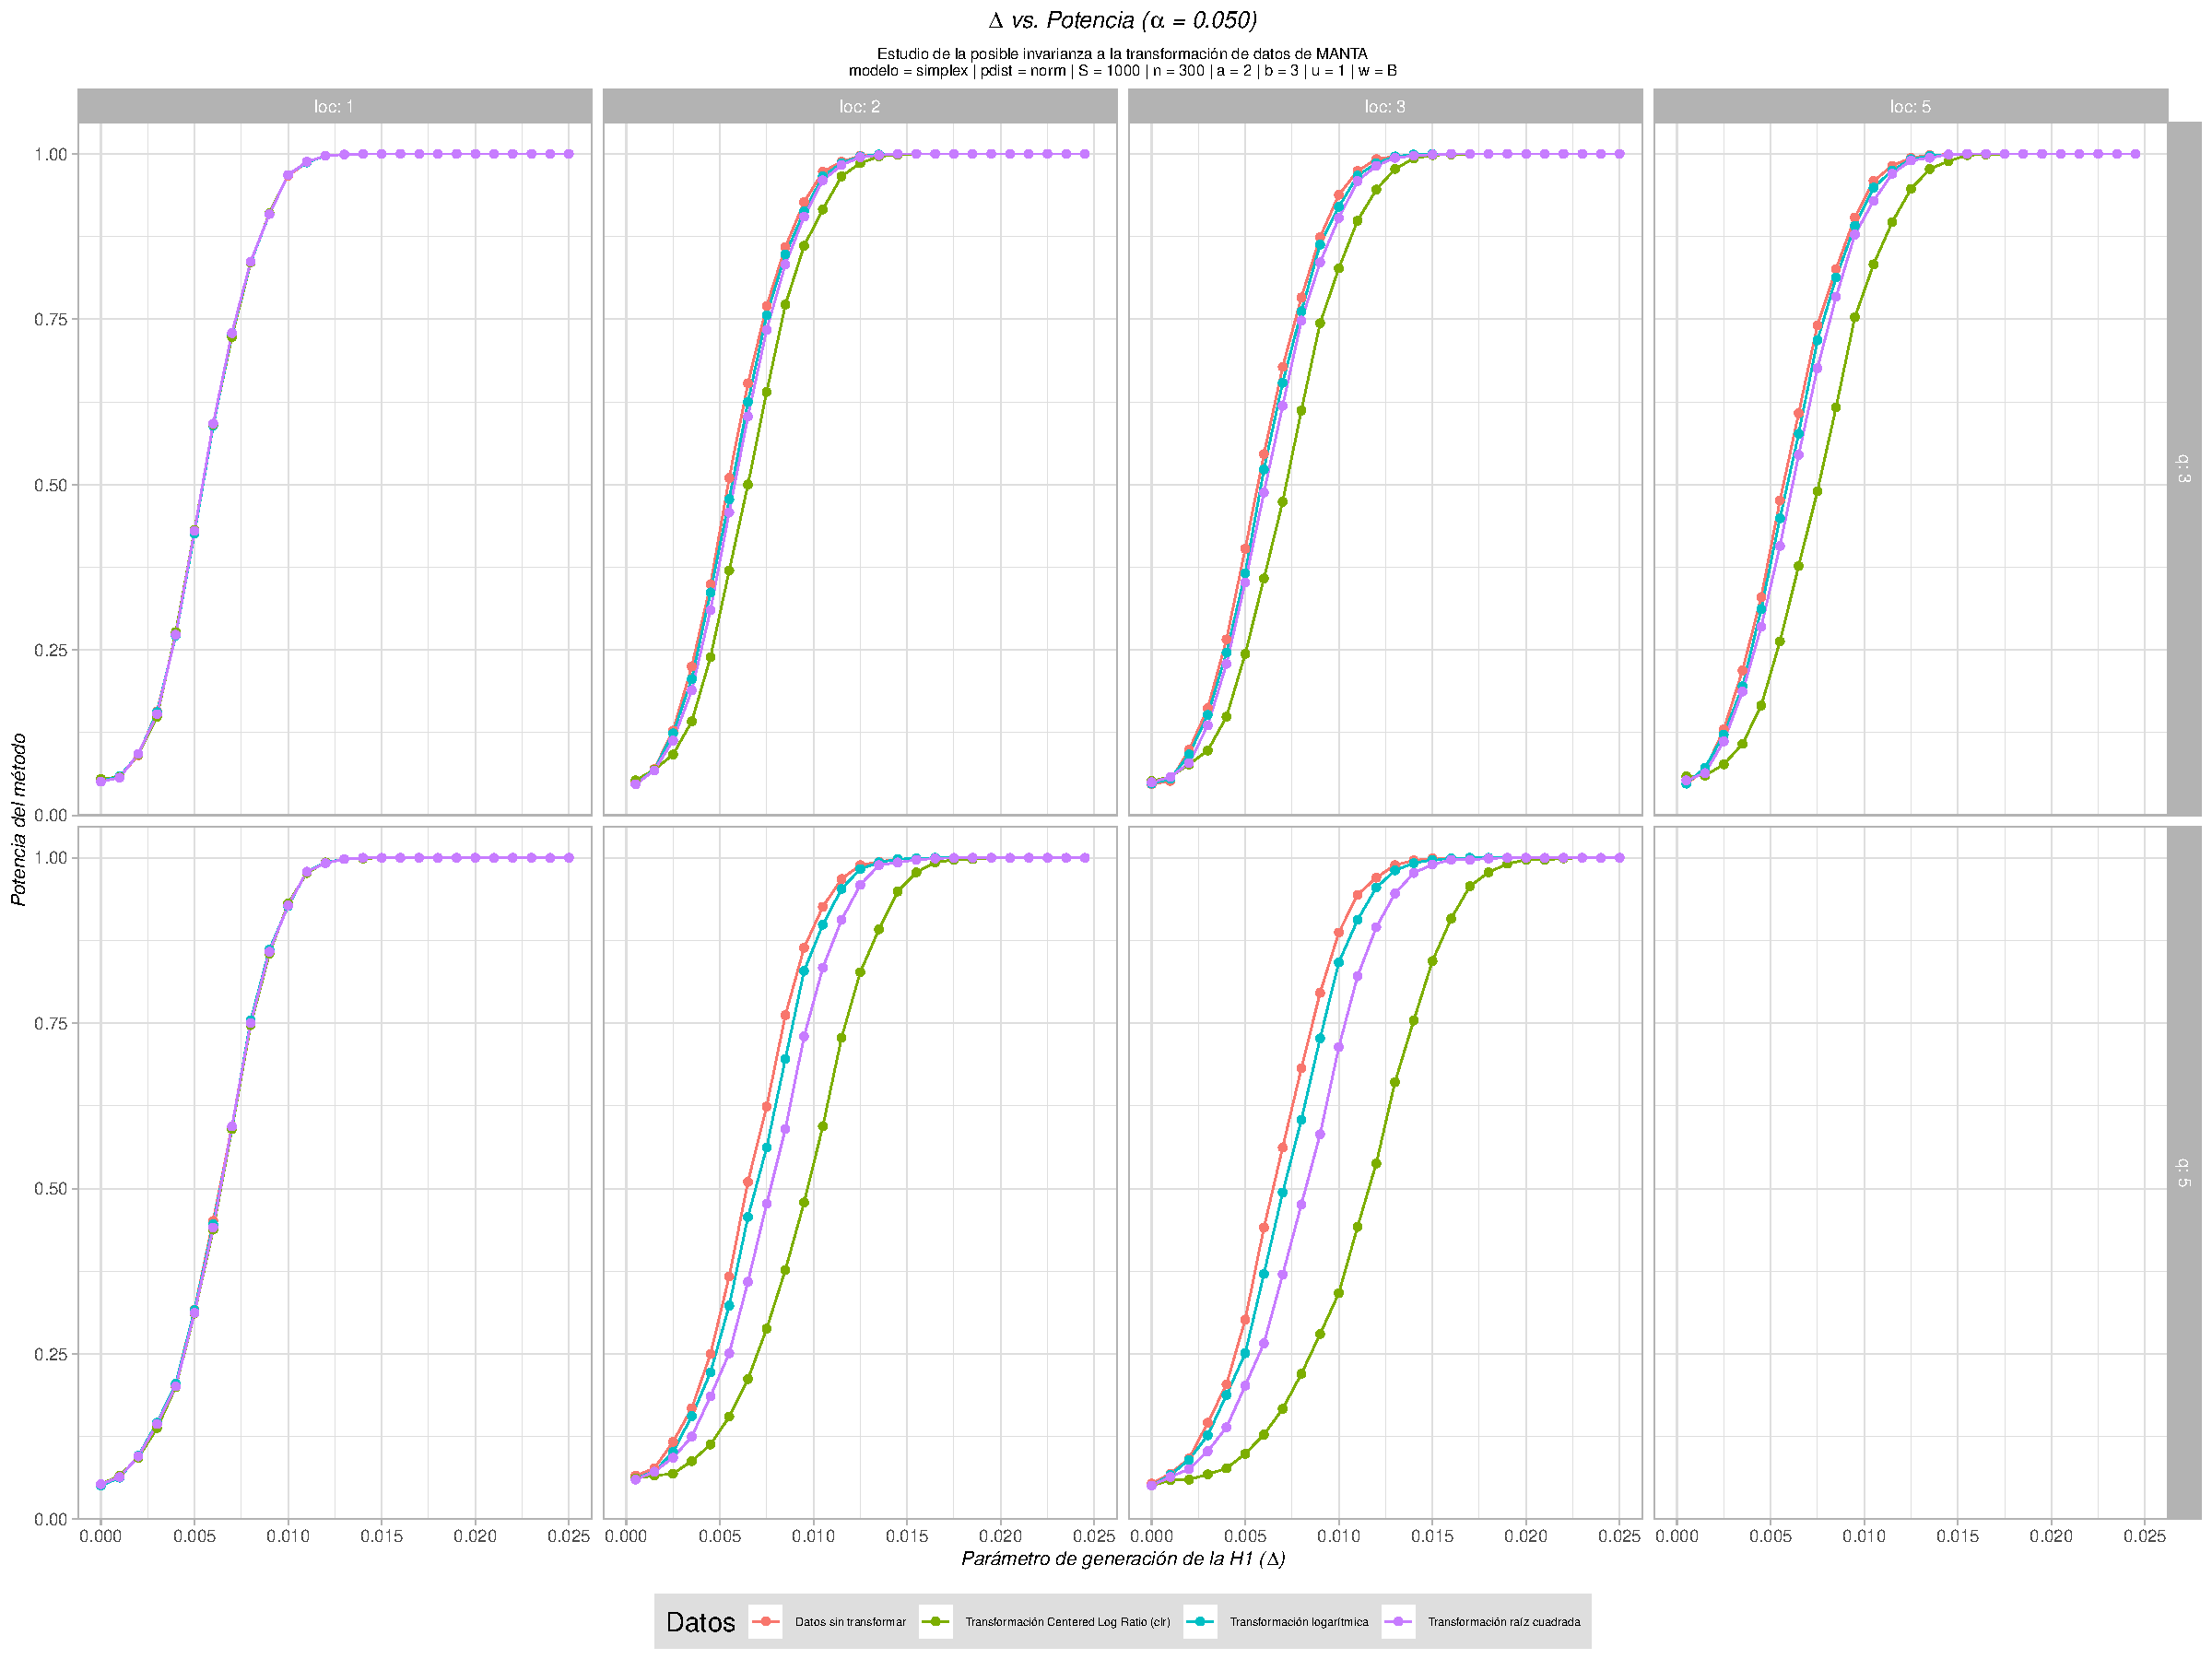
\includegraphics[scale=.45]{OBJ2SimplexMANTAqloc005.pdf}
    \caption{\scriptsize{A.}}
    \label{fig:OBJ2SimplexMANTAqloc005}
\end{figure}

% OBJ2SimplexMANTAqloc005ColaIzq.pdf
% OBJ2SimplexMANTAqloc005Coladch.pdf
\begin{figure}[!htbp]
\hspace*{-2cm} % Movimiento relativo del gráfico
\begin{subfigure}{.65\textwidth}
  \centering
  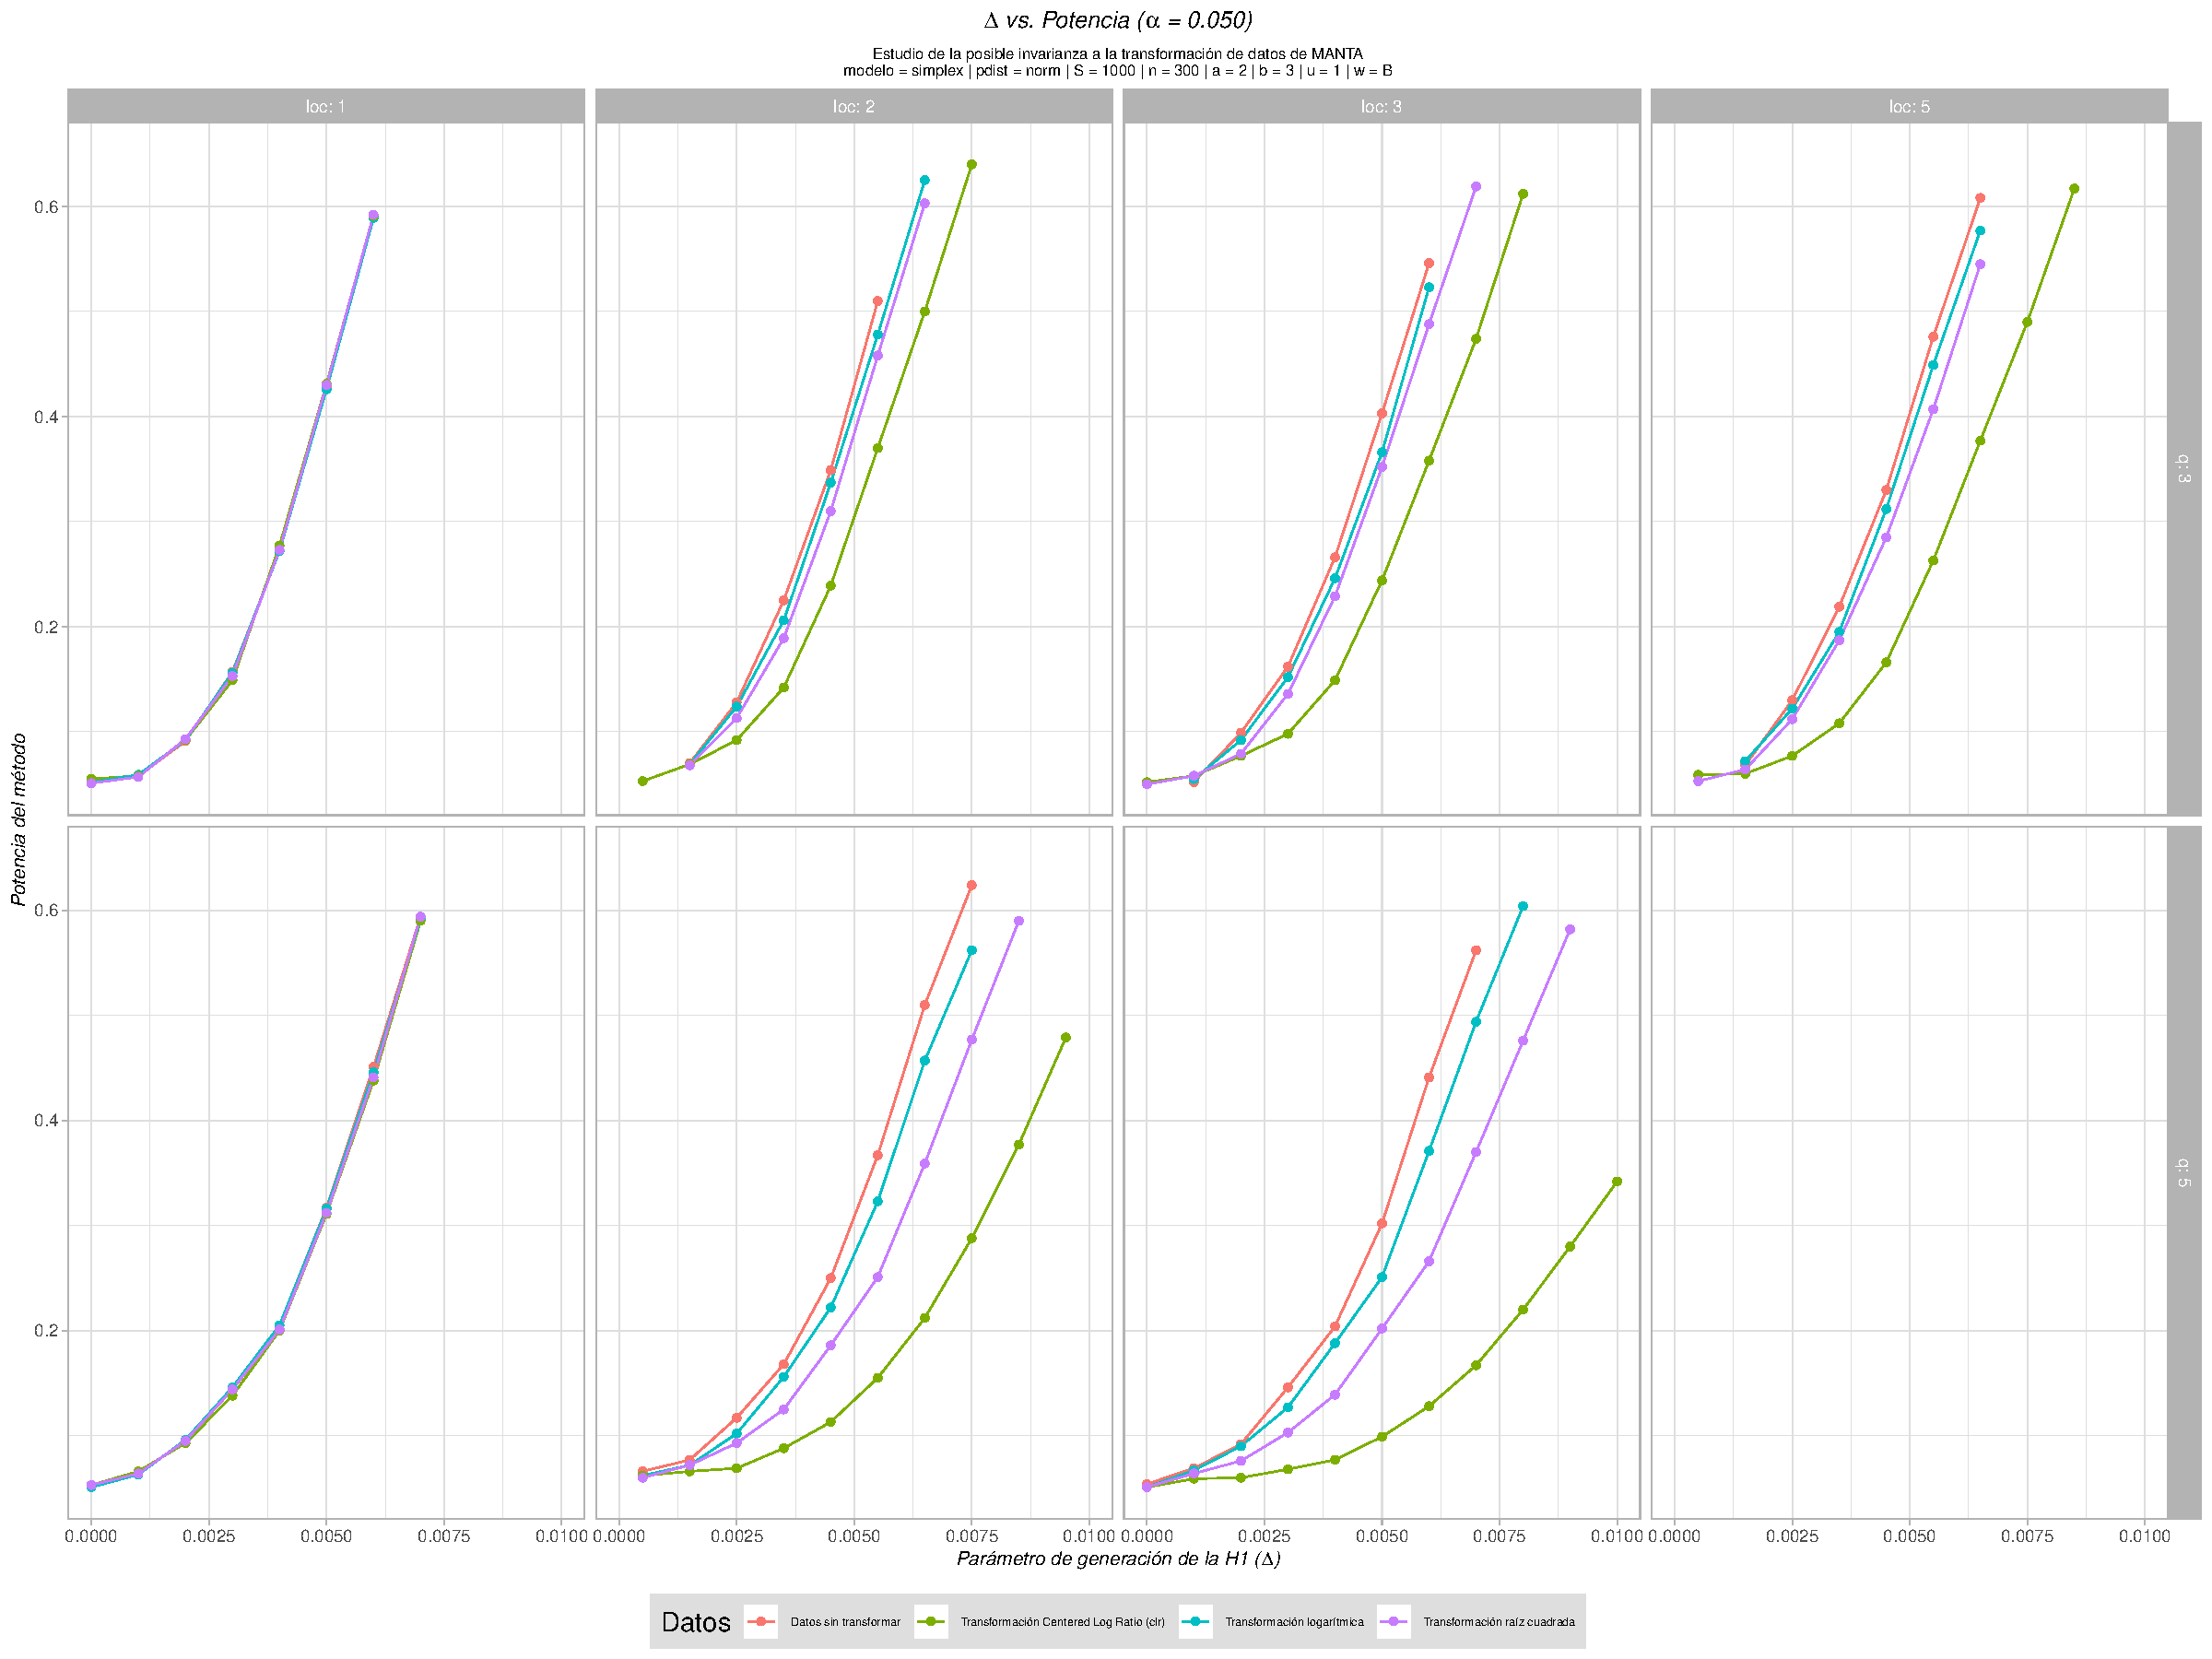
\includegraphics[width=.7\linewidth]{OBJ2SimplexMANTAqloc005ColaIzq.pdf}
  \caption{\scriptsize{A.}}
  \label{fig:OBJ2SimplexMANTAqloc005ColaIzq}
\end{subfigure}%
\begin{subfigure}{.65\textwidth}
\hspace*{-2.3cm} % Movimiento relativo del gráfico
  \centering
  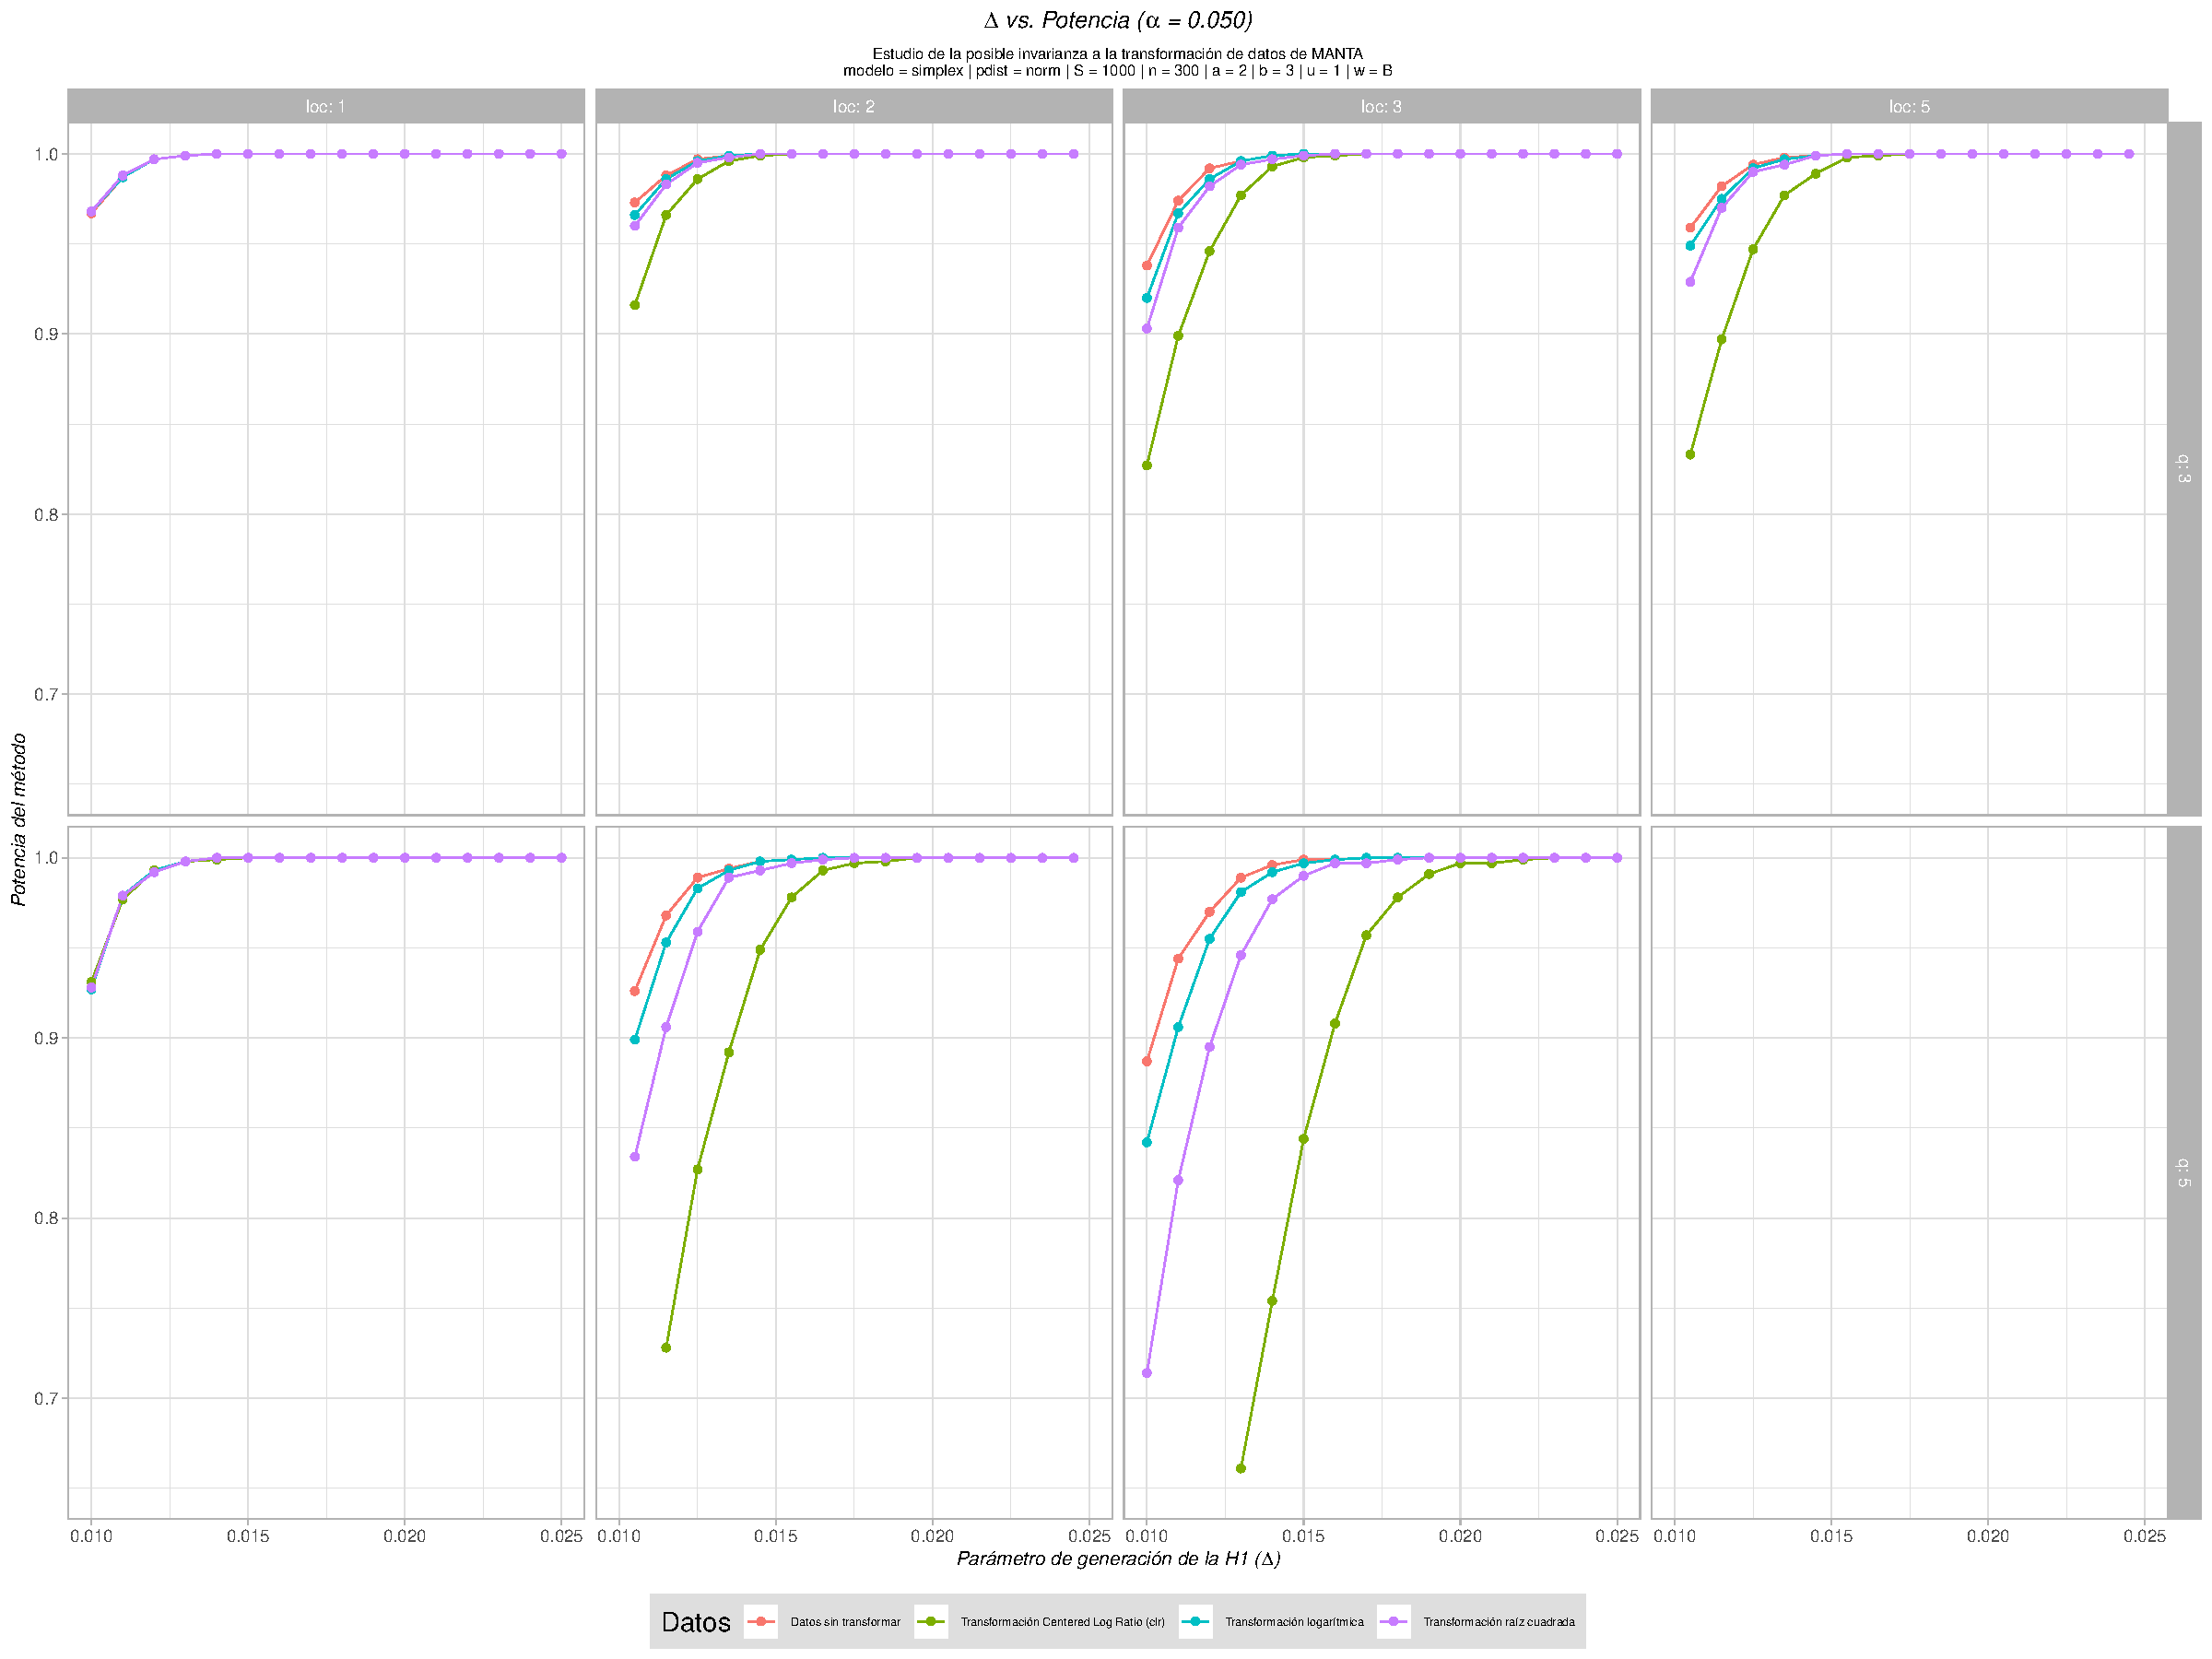
\includegraphics[width=.7\linewidth]{OBJ2SimplexMANTAqloc005Coladch.pdf}
  \caption{\scriptsize{A.}}
  \label{fig:OBJ2SimplexMANTAqloc005Coladch}
\end{subfigure}
\caption{\scriptsize{A.}}
\label{fig:OBJ2005zoom}
\end{figure}

Como ya se avanzó en el detallado del segundo objetivo en la sección \textit{\ref{sec:Objetivos finales del estudio}}, se repitieron las simulaciones anteriores pero realizando el cálculo de \( \mathbb P \) bajo niveles de significación más bajos, en particular: \( \alpha \in [\text{0.01}, \text{0.001}]] \)

Similarmente al caso previo, para \( \alpha = \text{0.01} \) se obtuvieron las figuras \ref{fig:OBJ2SimplexMANTAqloc001} y \ref{fig:OBJ2001zoom}, y para \( \alpha = \text{0.001} \) los gráficos que se encuentran disponibles en \ref{fig:OBJ2SimplexMANTAqloc0001}, \ref{fig:OBJ20001zoom}.

% OBJ2SimplexMANTAqloc001.pdf
\begin{figure}[!htbp]
\hspace*{-0.8cm} % Movimiento relativo del gráfico
    \centering
    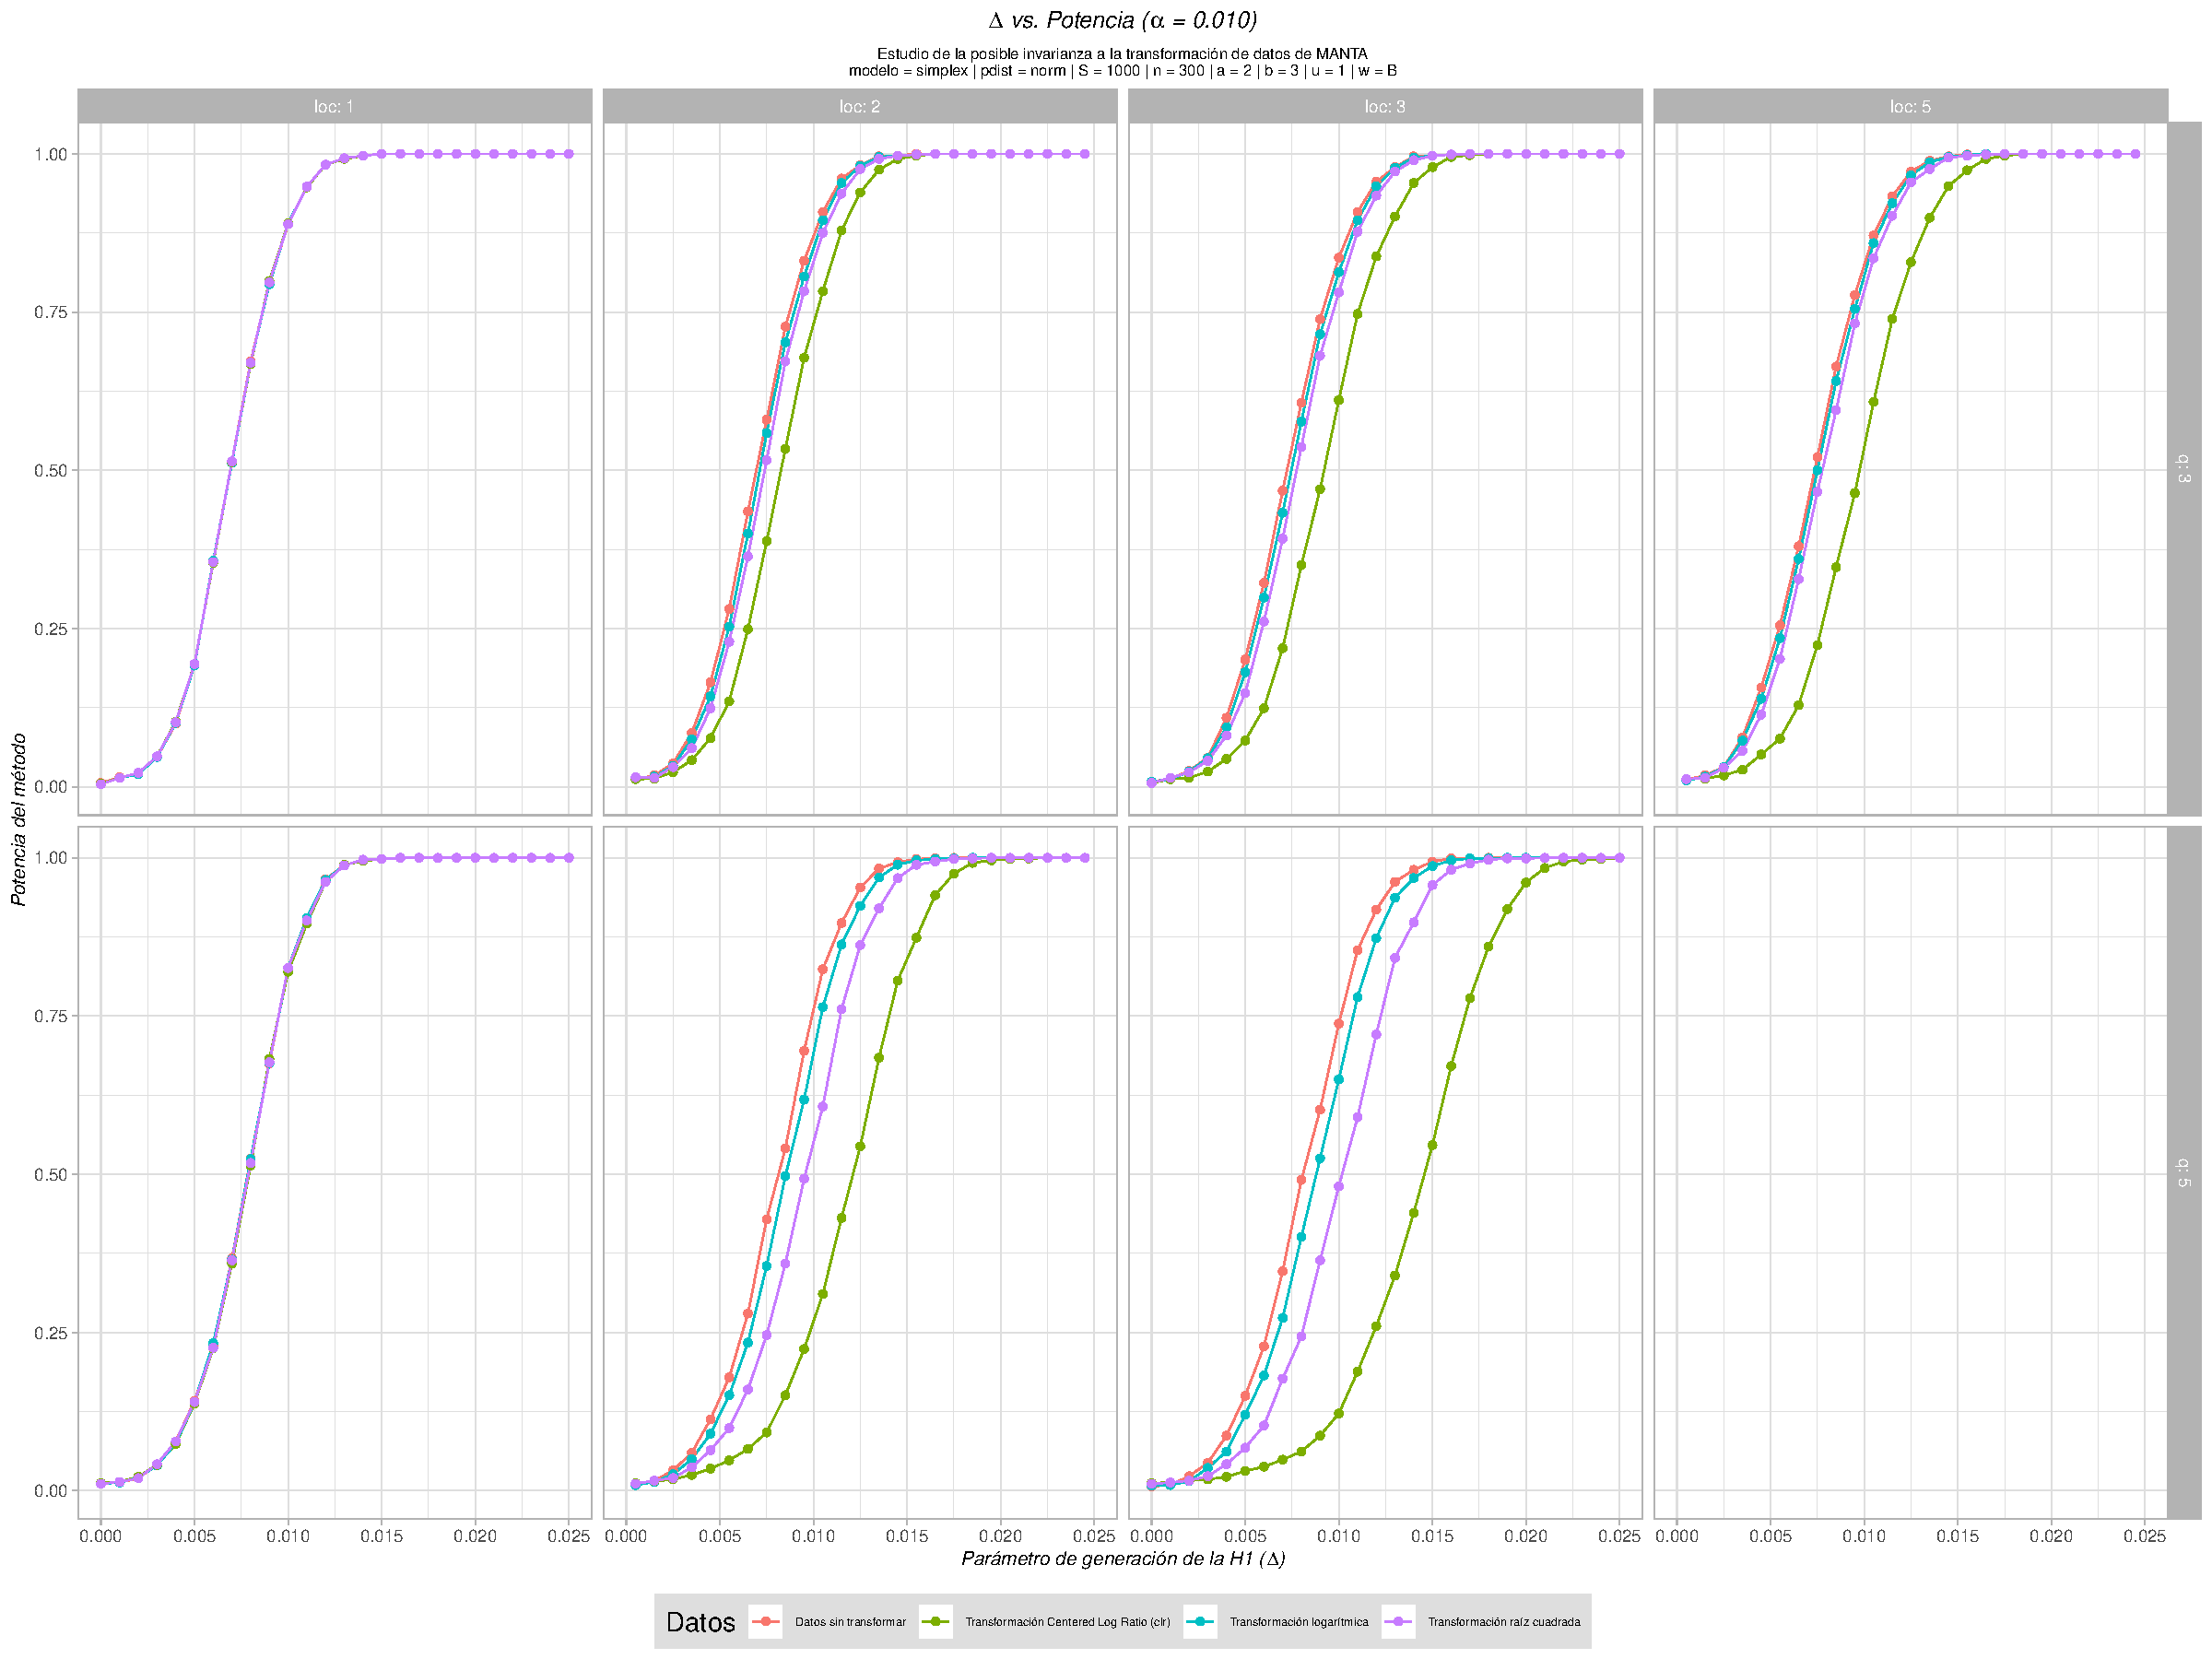
\includegraphics[scale=.45]{OBJ2SimplexMANTAqloc001.pdf}
    \caption{\scriptsize{A.}}
    \label{fig:OBJ2SimplexMANTAqloc001}
\end{figure}

% OBJ2SimplexMANTAqloc001ColaIzq.pdf
% OBJ2SimplexMANTAqloc001Coladch.pdf
\begin{figure}[!htbp]
\hspace*{-2cm} % Movimiento relativo del gráfico
\begin{subfigure}{.65\textwidth}
  \centering
  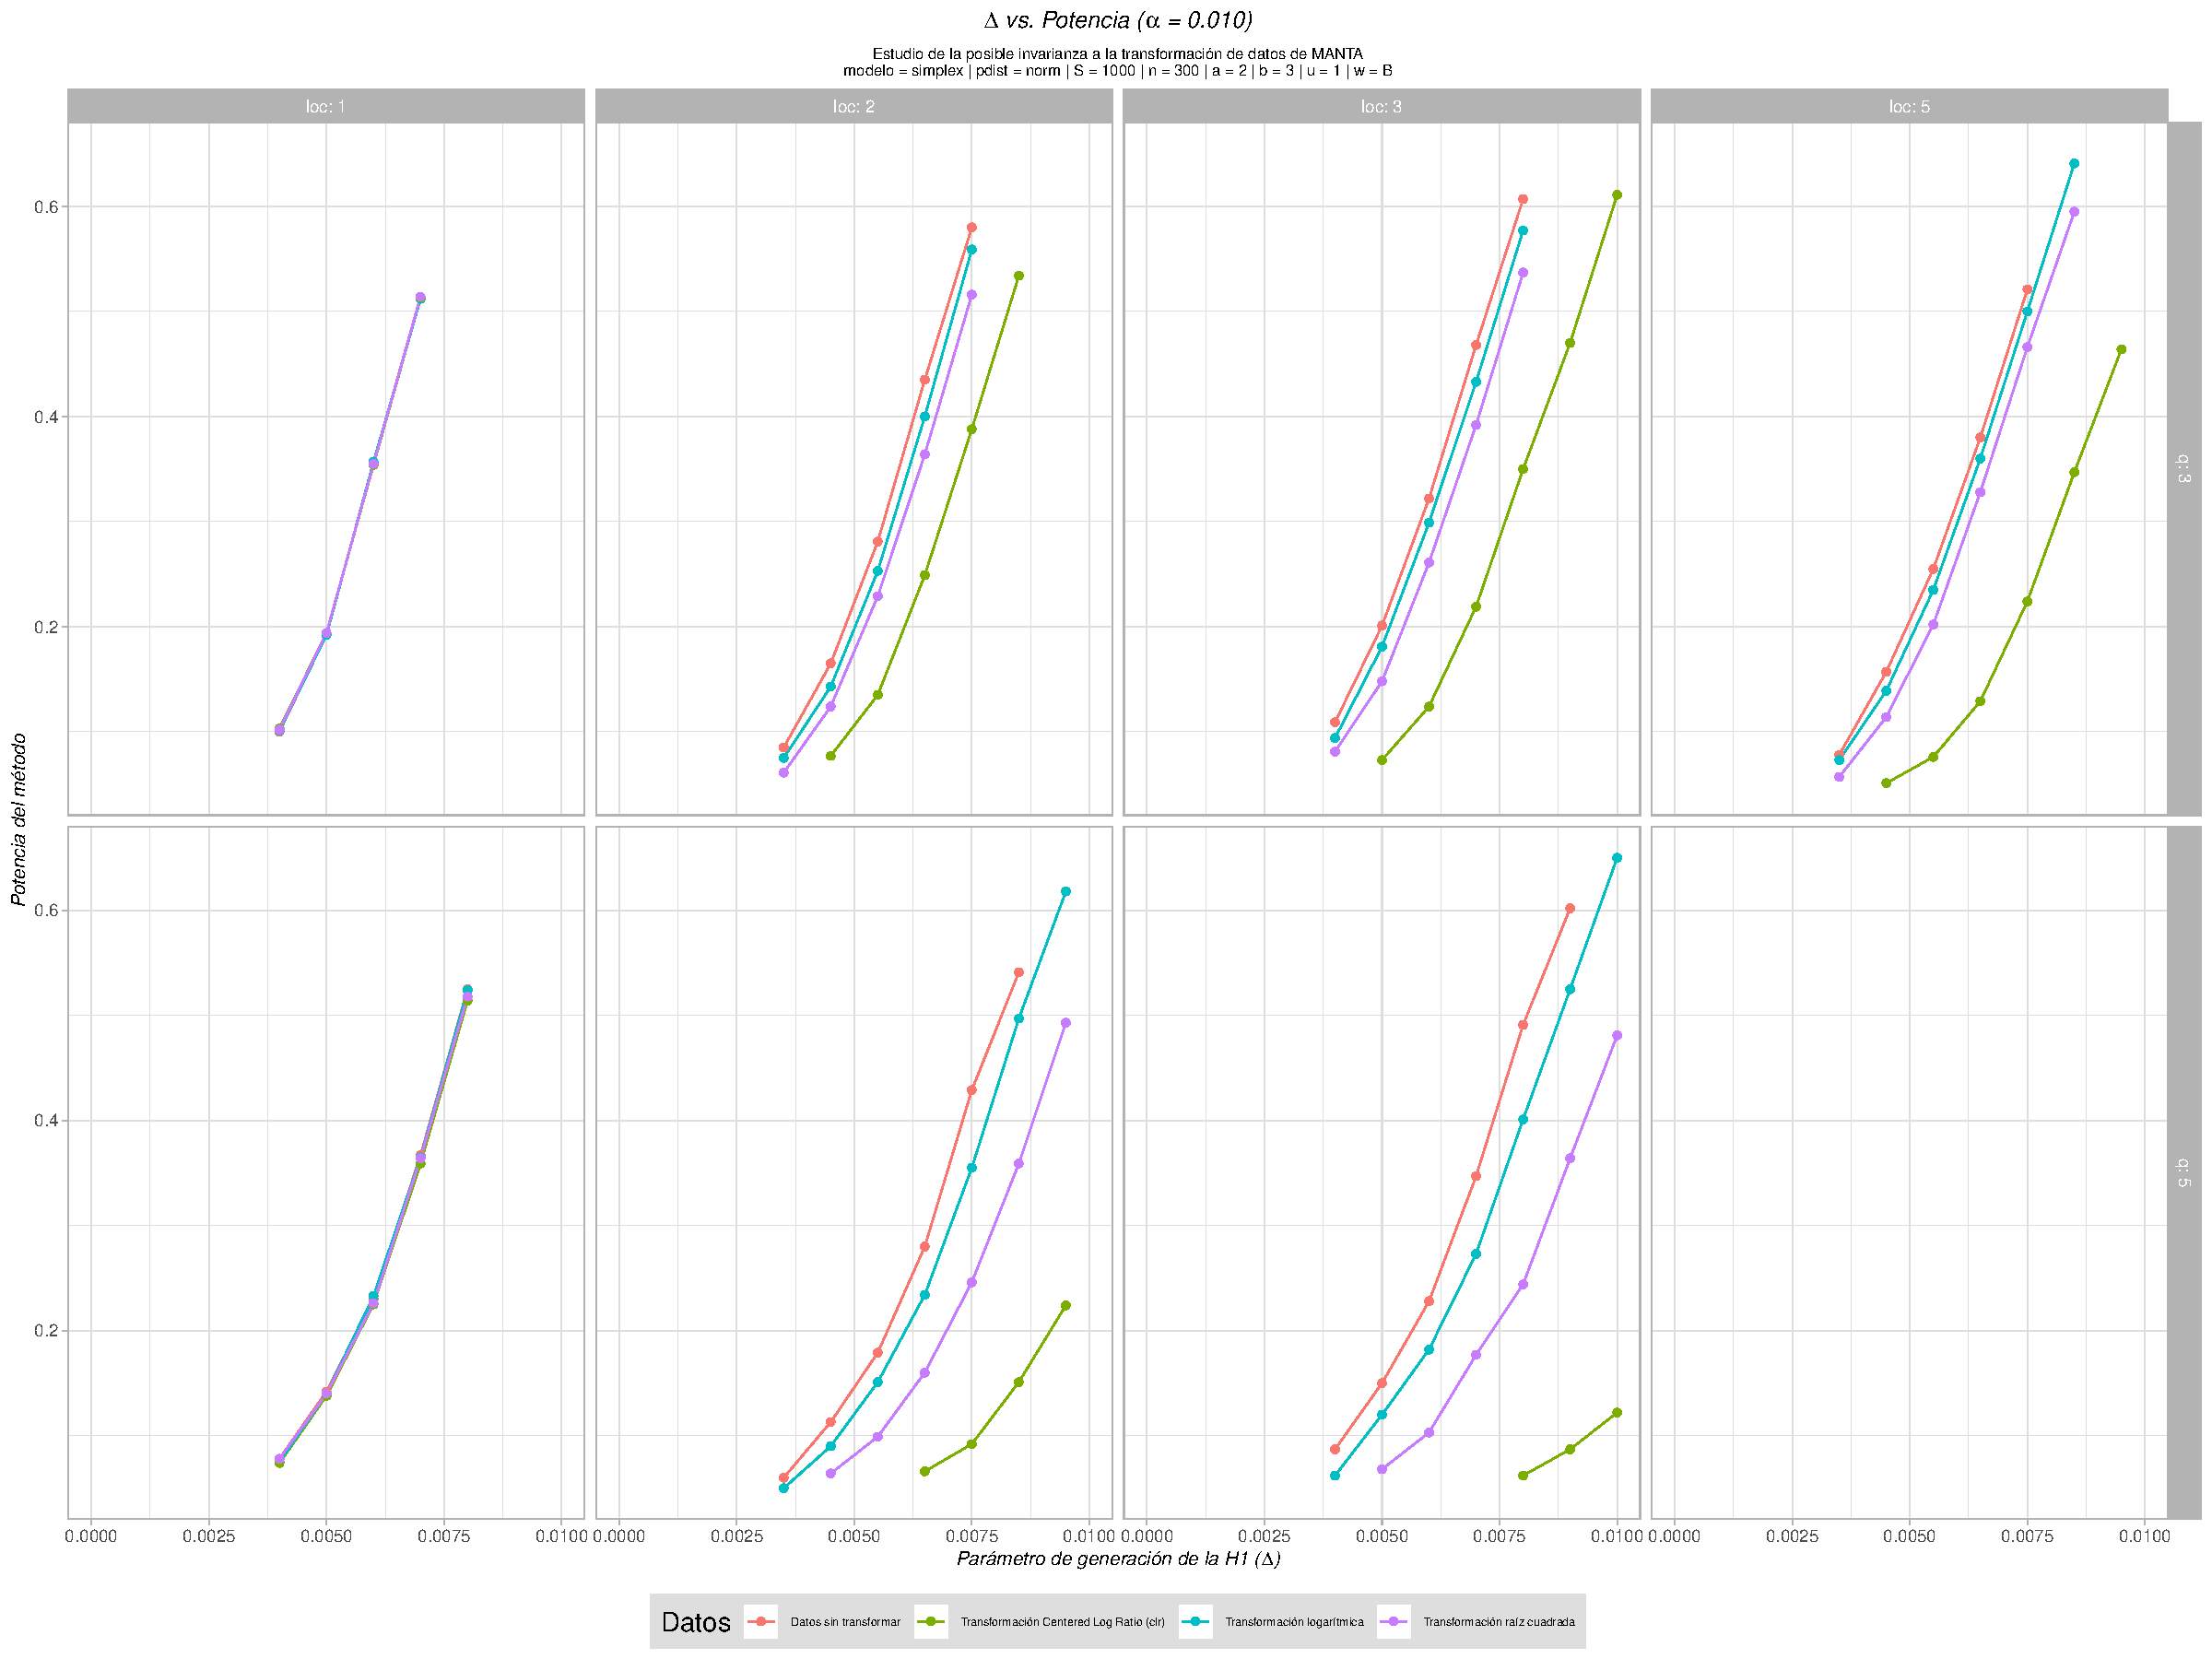
\includegraphics[width=.7\linewidth]{OBJ2SimplexMANTAqloc001ColaIzq.pdf}
  \caption{\scriptsize{A.}}
  \label{fig:OBJ2SimplexMANTAqloc001ColaIzq}
\end{subfigure}%
\begin{subfigure}{.65\textwidth}
\hspace*{-2.3cm} % Movimiento relativo del gráfico
  \centering
  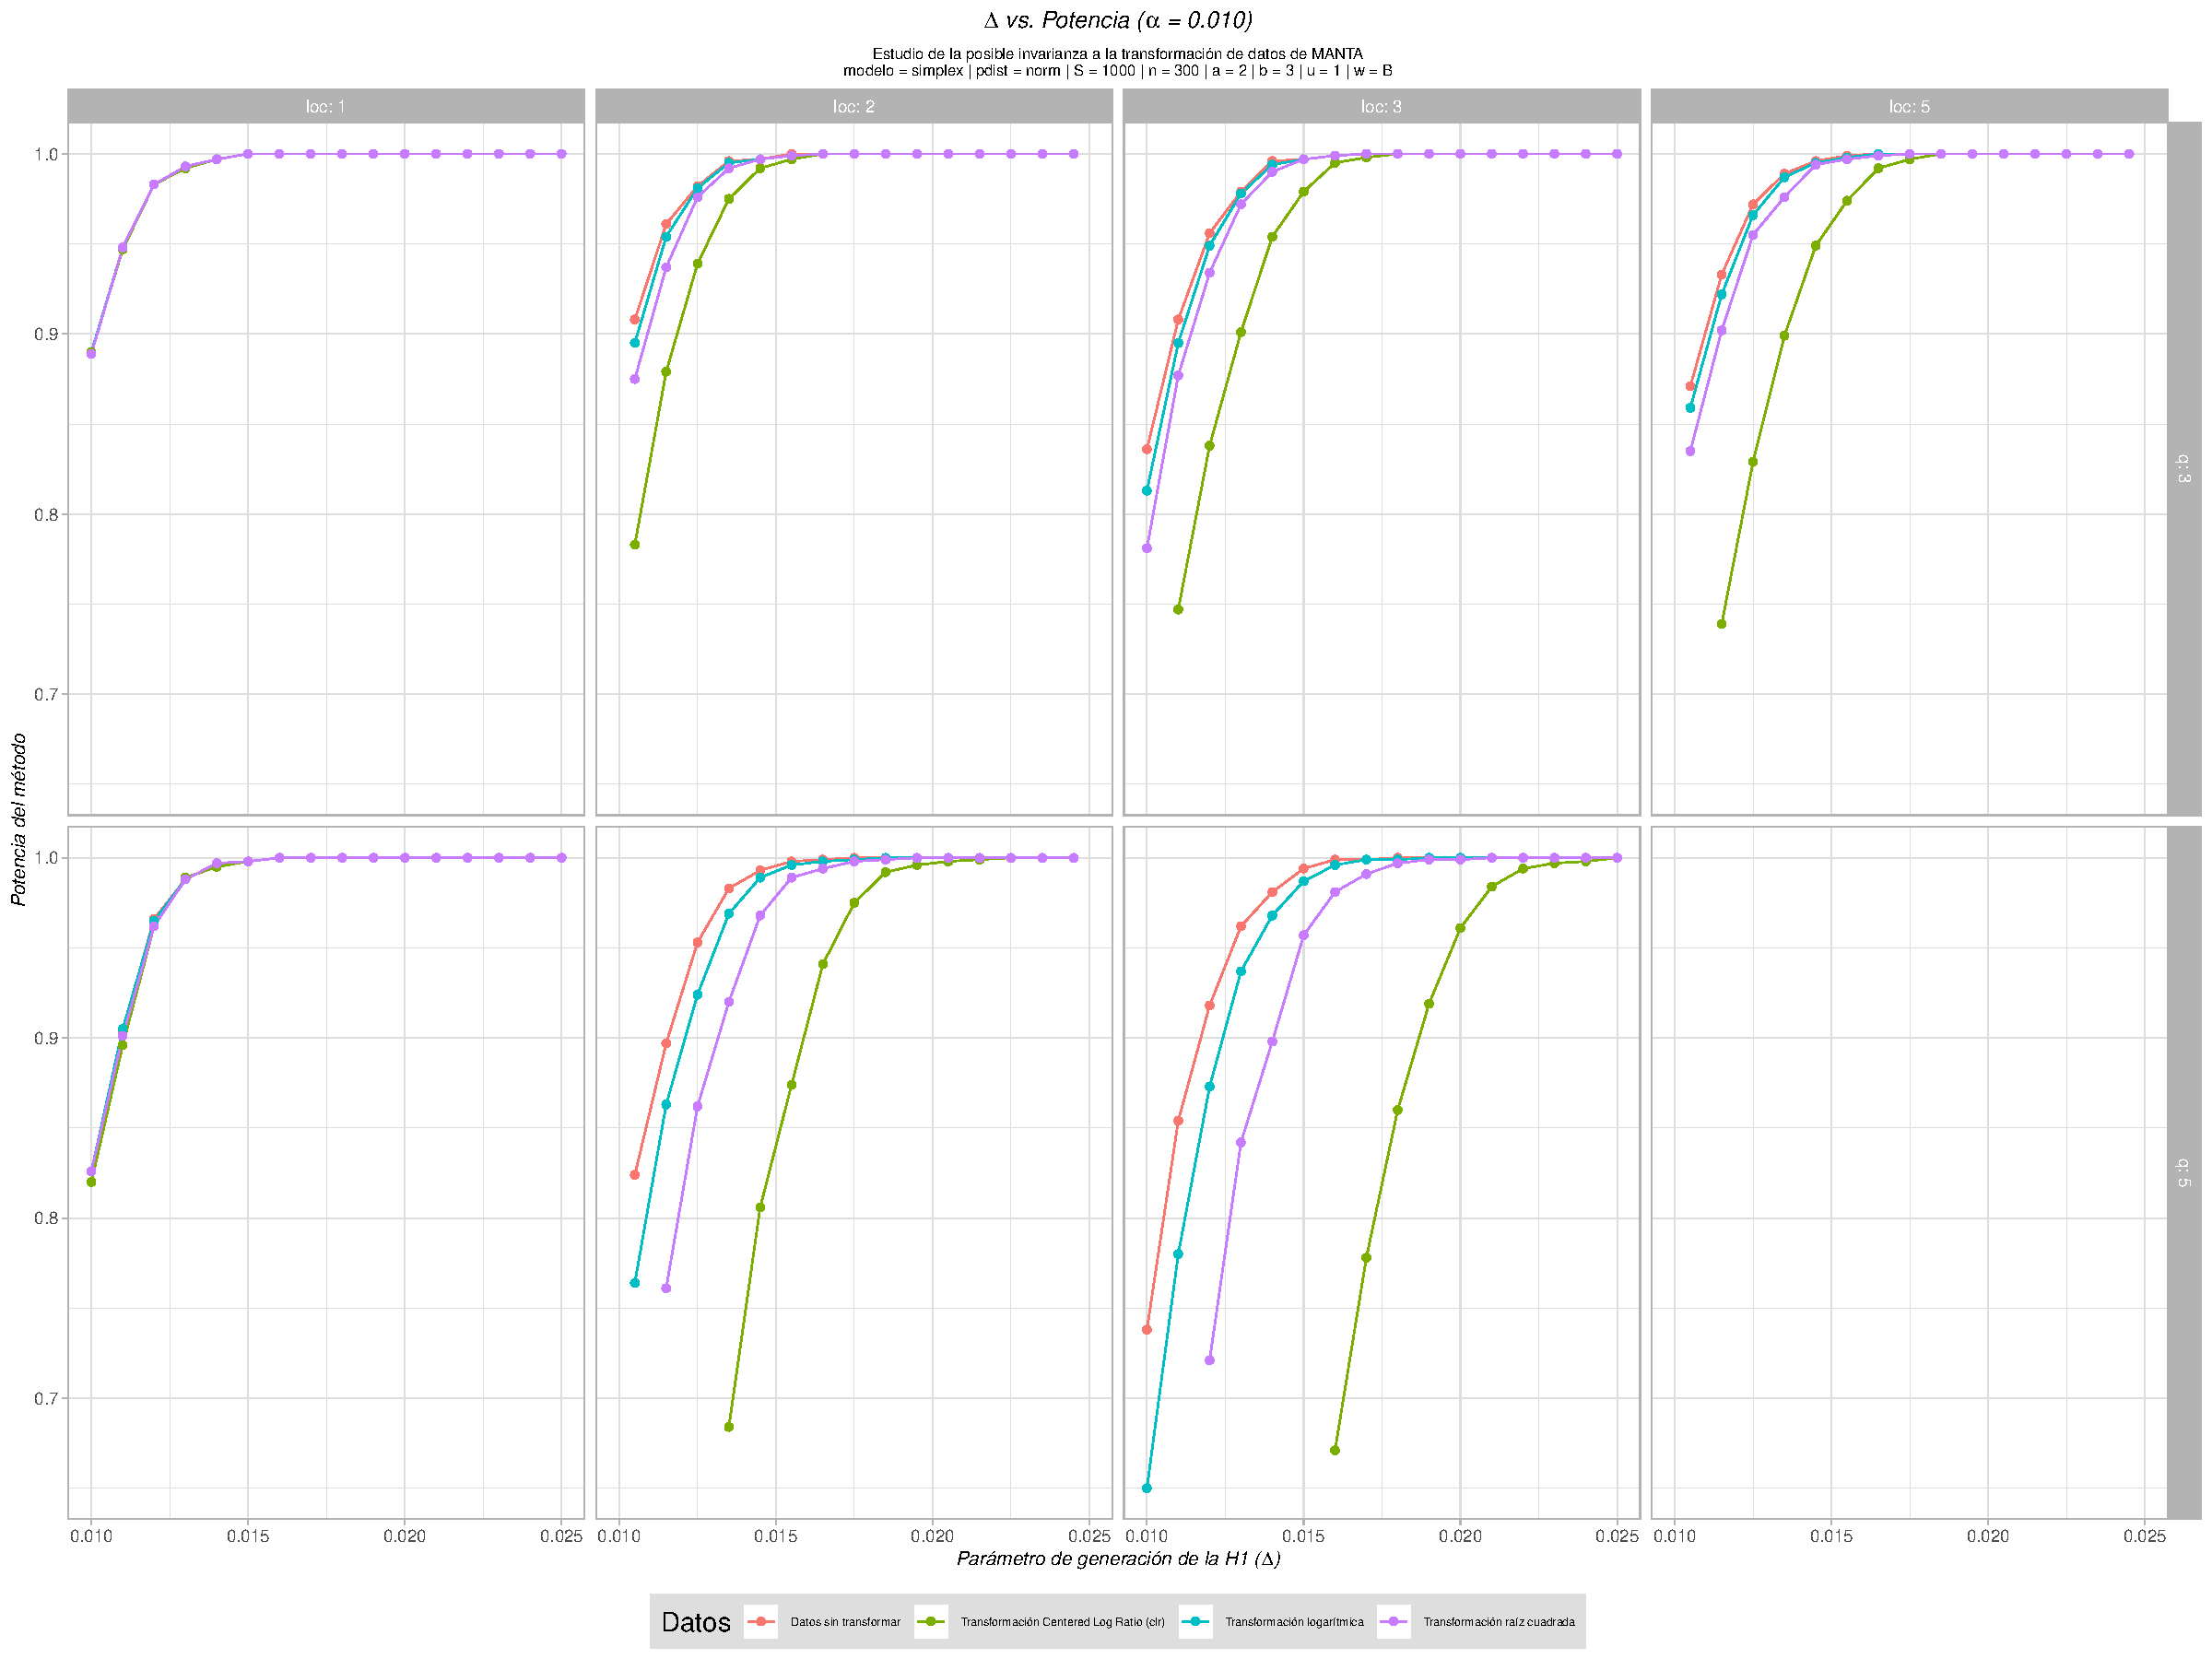
\includegraphics[width=.7\linewidth]{OBJ2SimplexMANTAqloc001Coladch.pdf}
  \caption{\scriptsize{A.}}
  \label{fig:OBJ2SimplexMANTAqloc001Coladch}
\end{subfigure}
\caption{\scriptsize{A.}}
\label{fig:OBJ2001zoom}
\end{figure}

% OBJ2SimplexMANTAqloc0001.pdf
\begin{figure}[!htbp]
\hspace*{-0.8cm} % Movimiento relativo del gráfico
    \centering
    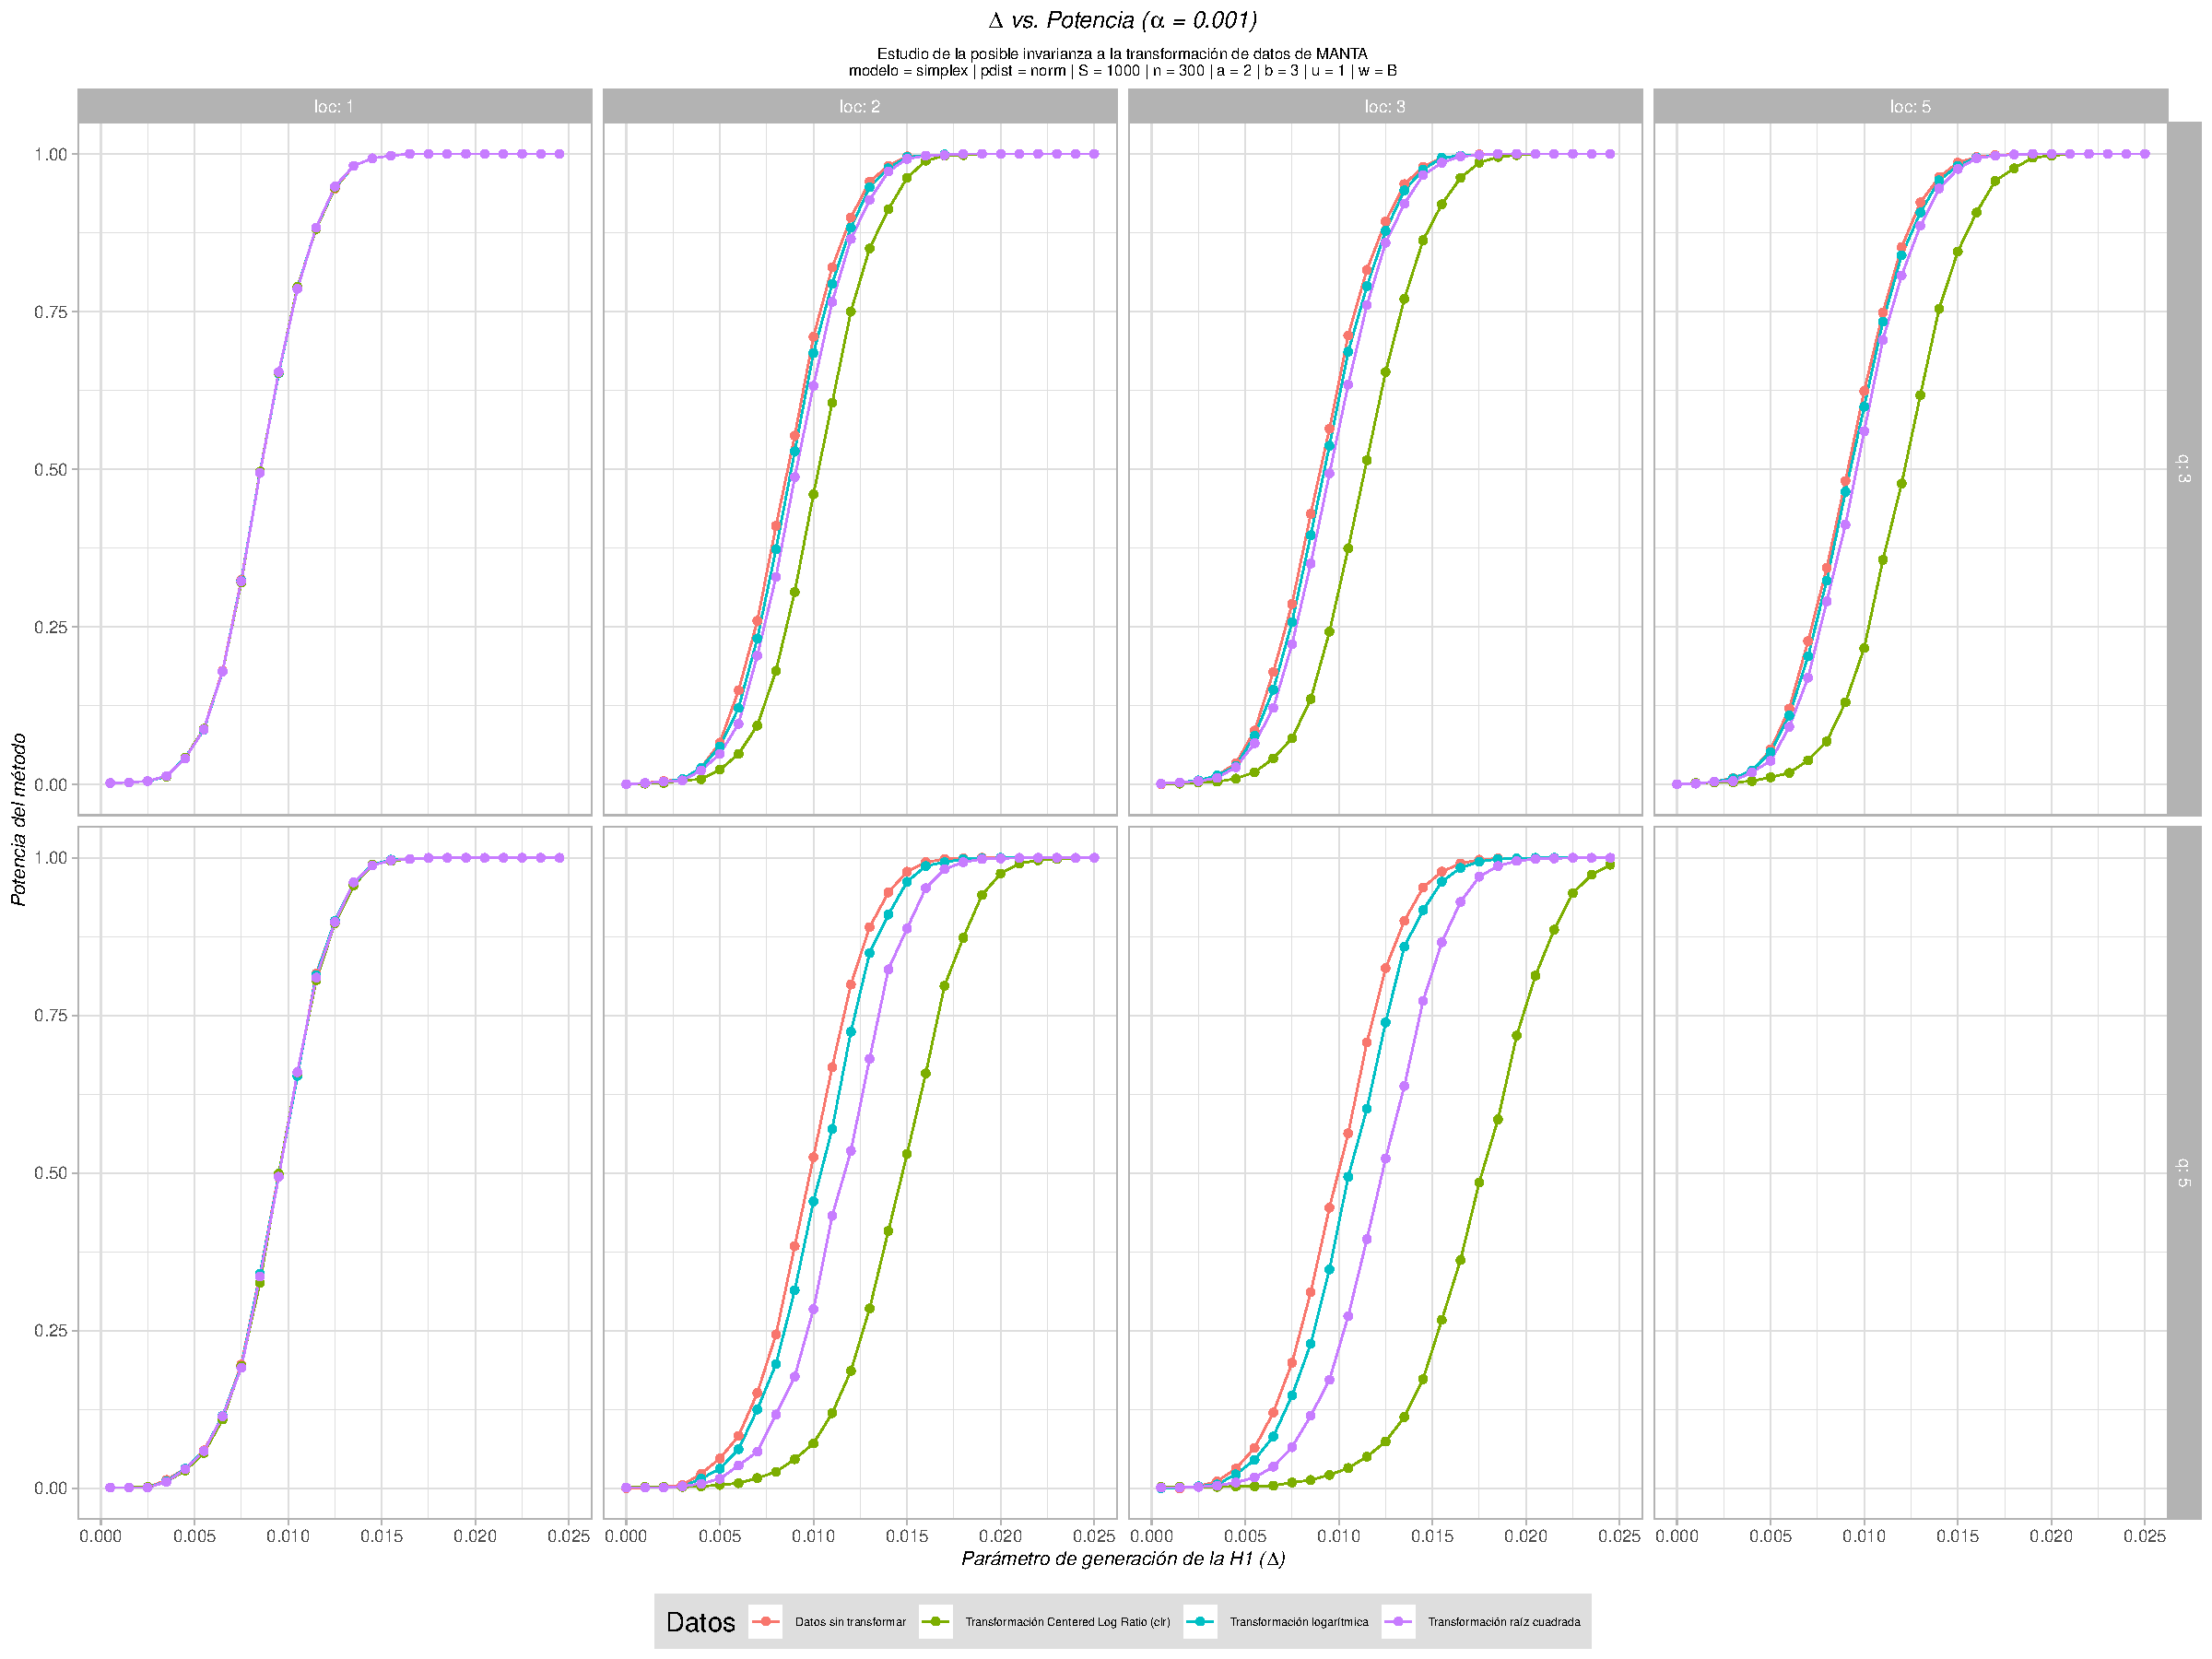
\includegraphics[scale=.45]{OBJ2SimplexMANTAqloc0001.pdf}
    \caption{\scriptsize{A.}}
    \label{fig:OBJ2SimplexMANTAqloc0001}
\end{figure}

% OBJ2SimplexMANTAqloc0001ColaIzq.pdf
% OBJ2SimplexMANTAqloc0001Coladch.pdf
\begin{figure}[!htbp]
\hspace*{-2cm} % Movimiento relativo del gráfico
\begin{subfigure}{.65\textwidth}
  \centering
  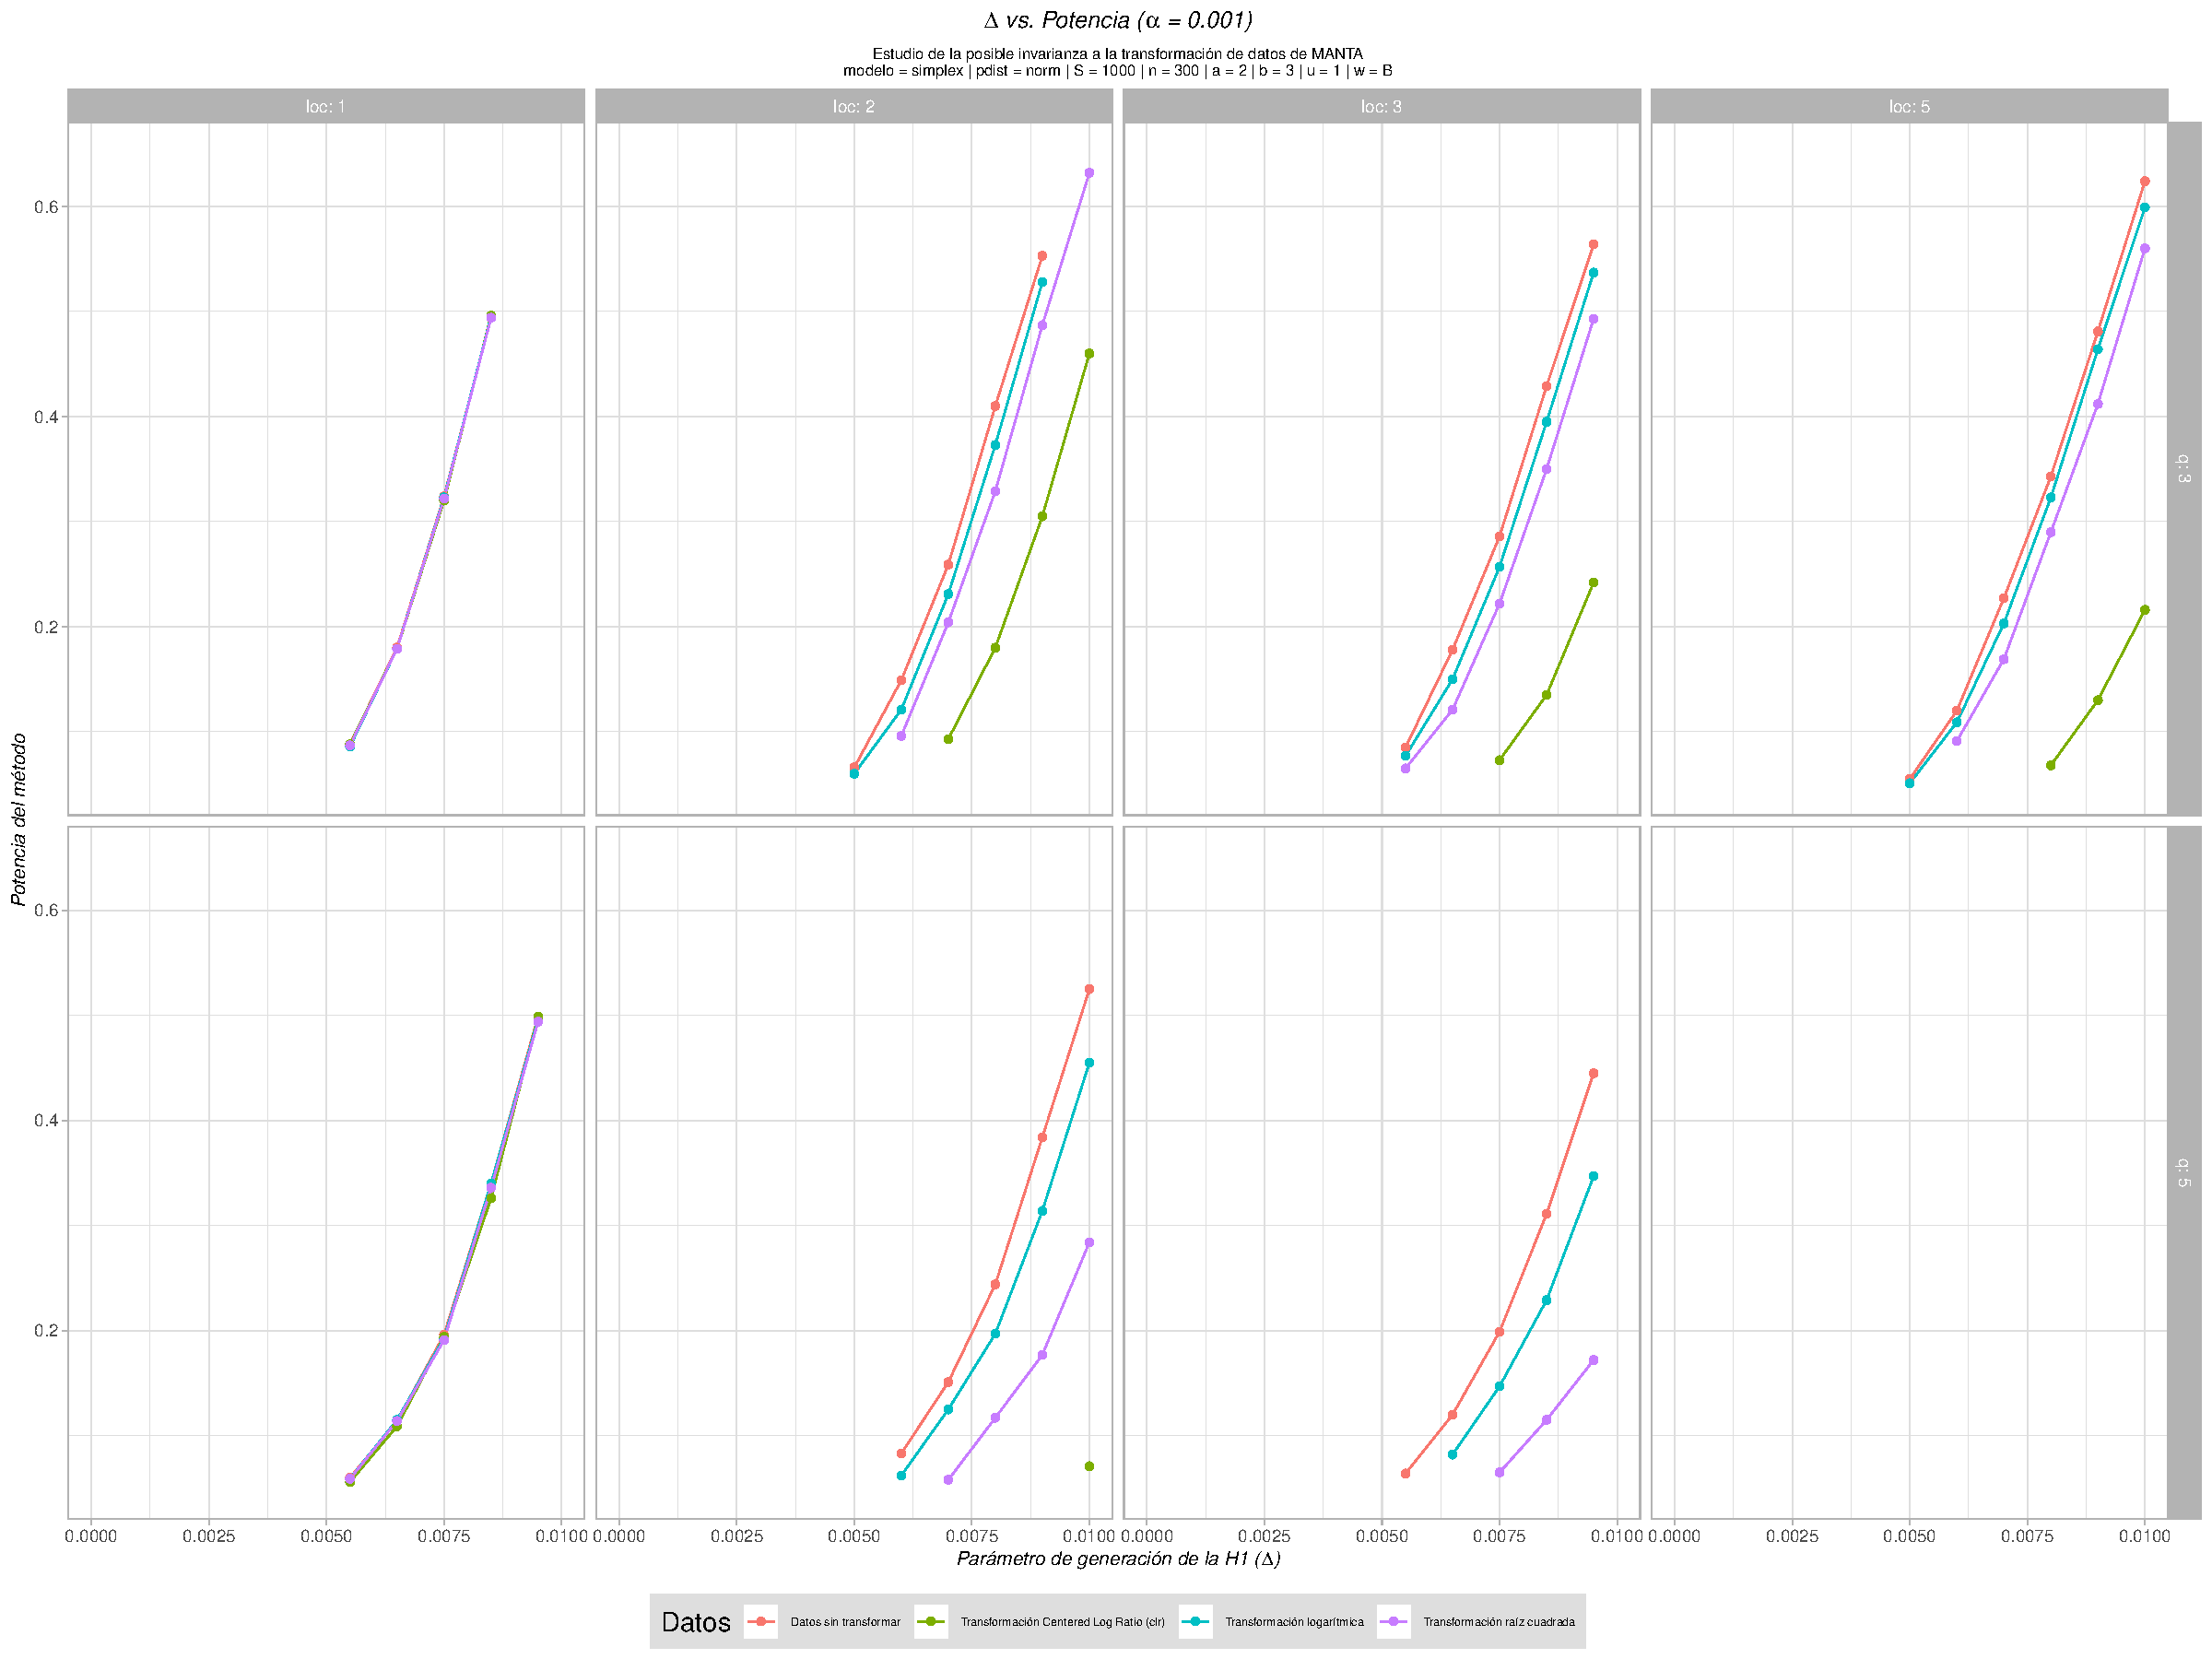
\includegraphics[width=.7\linewidth]{OBJ2SimplexMANTAqloc0001ColaIzq.pdf}
  \caption{\scriptsize{A.}}
  \label{fig:OBJ2SimplexMANTAqloc0001ColaIzq}
\end{subfigure}%
\begin{subfigure}{.65\textwidth}
\hspace*{-2.3cm} % Movimiento relativo del gráfico
  \centering
  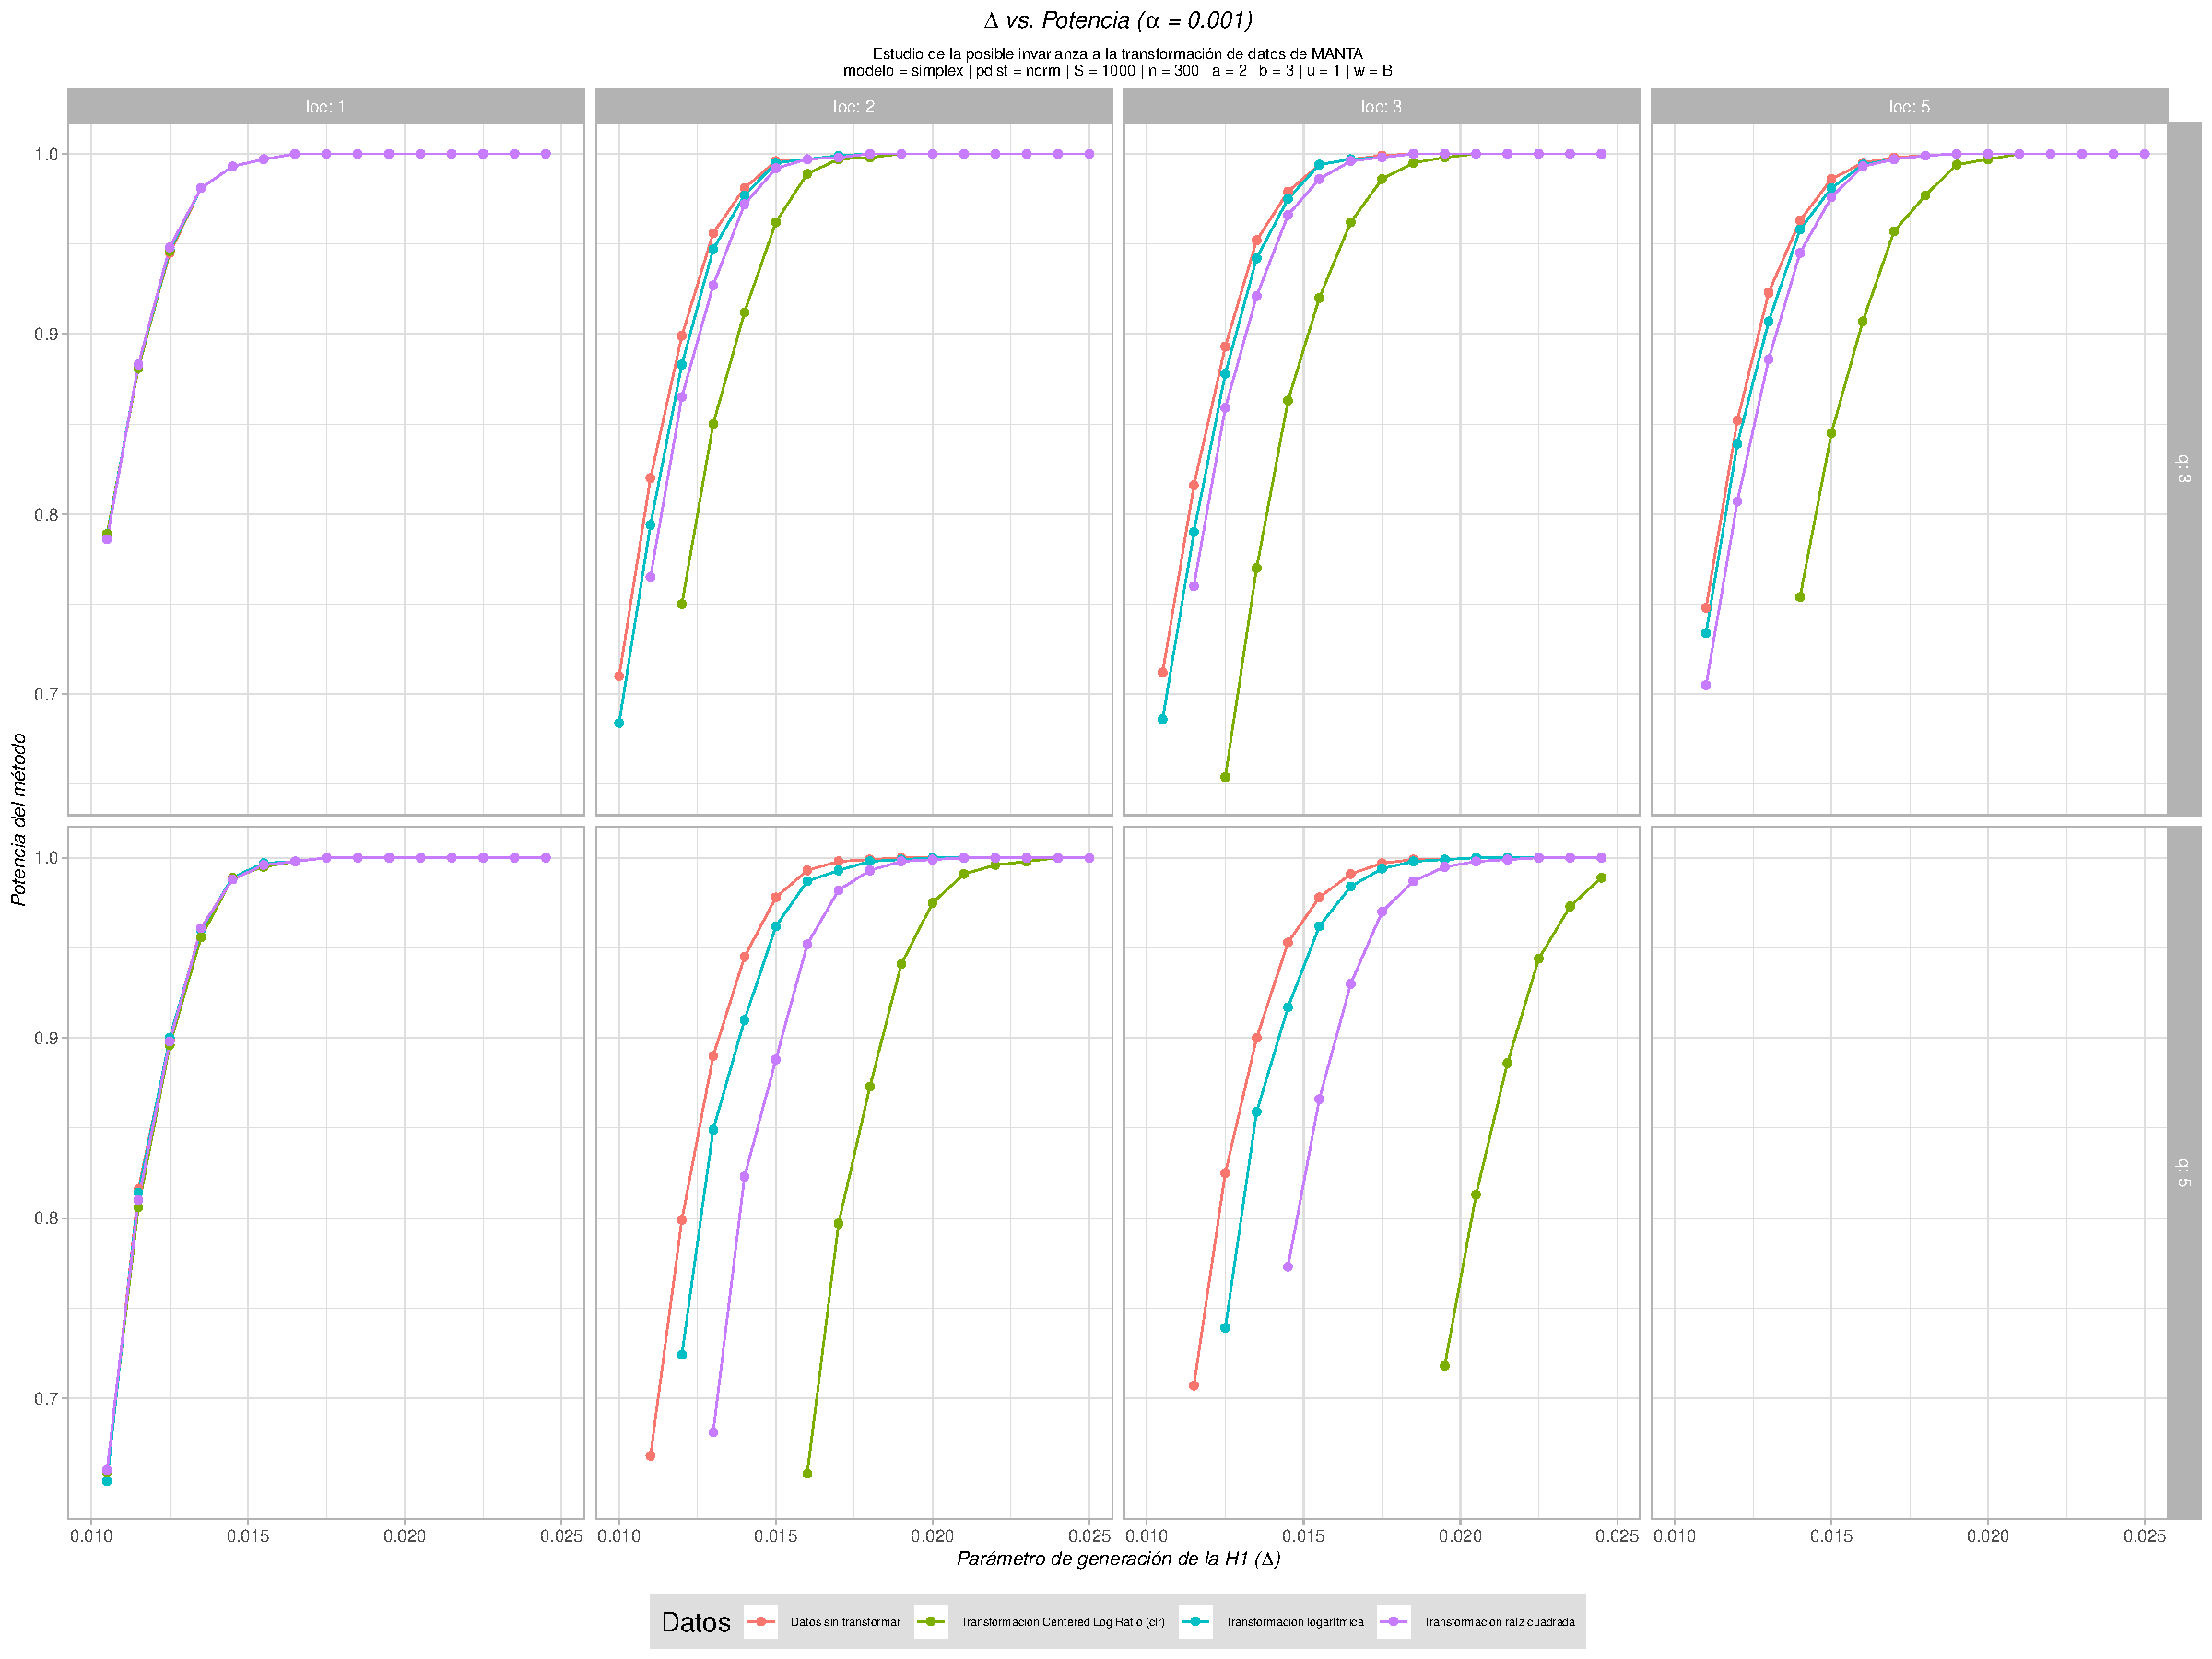
\includegraphics[width=.7\linewidth]{OBJ2SimplexMANTAqloc0001Coladch.pdf}
  \caption{\scriptsize{A.}}
  \label{fig:OBJ2SimplexMANTAqloc0001Coladch}
\end{subfigure}
\caption{\scriptsize{A.}}
\label{fig:OBJ20001zoom}
\end{figure}


\chapter{Discusión}
\label{chap:Discusión}

% Discusión de los resultados en el contexto del proyecto. Es en este apartado donde cobran sentido y en el cual se responden las preguntas de investigación y se muestra cómo los resultados dan respuesta a los problemas planteados.

...


%%%%%%%%%%%%%%%%%%%%%%%%%%%%%%%%%%%%%%%%%%%%%%%%%%%%%%%%%%%%%%%%%%%%%%%%%%%%%
% Cuarta parte: Conclusión + Retoques (Glosario, seguimiento...)  <--> PEC4 %
%%%%%%%%%%%%%%%%%%%%%%%%%%%%%%%%%%%%%%%%%%%%%%%%%%%%%%%%%%%%%%%%%%%%%%%%%%%%%


\chapter{Conclusiones y trabajos futuros}
\label{chap:Conclusiones y trabajos futuros}

\section{Conclusiones}
\label{sec:Conclusiones}

% Este capítulo tiene que incluir:
% 
% \begin{itemize}
% \item Una descripción de las conclusiones del trabajo:
% \begin{itemize}
%     \item Una vez se han obtenido los resultados, ¿qué conclusiones se extraen?
%     \item ¿Estos resultados son los esperados? ¿O han sido sorprendentes? ¿Por qué?
% \end{itemize}
% \item Una reflexión crítica sobre el logro de los objetivos planteados inicialmente:
% \begin{itemize}
%     \item ¿Hemos logrado todos los objetivos? Si la respuesta es negativa, ¿por qué motivo?
% \end{itemize}
% \end{itemize}

De los resultados obtenidos para los diferentes escenarios planteados en el presente estudio, disponibles en las distintas secciones del capítulo \textit{\hyperref[chap:Resultados]{Resultados}}, se puede resolver lo siguiente:

\begin{enumerate}[label=\textnormal{(\Roman*)}]
\item \label{th1} Primera conclusión...
\end{enumerate}


\section{Líneas de futuro}
\label{sec:Líneas de futuro}

% Las líneas de trabajo futuro que no se han podido explorar en este trabajo y han quedado pendientes.

Aunque solo sea por completitud del presente proyecto, preveemos como mínimo una línea de trabajo futuro: llevar a cabo el tercer objetivo planteado originalmente y que, por los motivos ya comentados anteriormente (\textit{\hyperref[sec:Desviaciones y acciones de mitigación]{Desviaciones y acciones de mitigación}} y \textit{\hyperref[sec:Análisis de riesgos]{Análisis de riesgos}}), no pudo llevarse a cabo.

Teniendo este punto en cuenta, y tras valorar los resultados obtenidos en el estudio cuantitativamente comparativo de la \textit{potencia estadística} (\( \mathbb P \)) de sendos métodos estadísticos multivariantes, \textit{MANOVA} y la versión asintótica de \textit{PERMANOVA}, se determina que:

\begin{enumerate}[label=\textnormal{(\Roman*)}]
\item \label{th1} Primera línea de trabajo futuro...
\end{enumerate}

\section{Seguimiento de la planificación}
\label{sec:Seguimiento de la planificación}

% \begin{itemize}
% \item
% Un análisis crítico del seguimiento de la planificación y metodología a lo largo del producto:
% \begin{itemize}
%     \item ¿Se ha seguido la planificación?
%     \item ¿La metodología prevista ha sido suficientemente adecuada?
%     \item ¿Ha habido que introducir cambios para garantizar el éxito del trabajo? ¿Por qué?
% \end{itemize}
% \item De los impactos previstos a \ref{s:etic}, ético-sociales, de sostenibilidad y de diversidad, avaluad/mencionad si se han mitigado (si eran negativos) o si se han conseguido (si eran positivos).
% \item Si han aparecido impactos no previstos en \ref{s:etic}, evaluar/mencionar cómo se han mitigado (si eran negativos) o que han aportado (si eran positivos).
% \end{itemize}

A modo de conclusión, se detallará el seguimiento real de la planificación original del trabajo, resaltando los escollos que fueron surgiendo, y las acciones de mitigación que se llevaron a cabo para subsanar los desvios que estos causaban en los tiempos estimados para cada tarea programada:

\begin{itemize}
\item A
\end{itemize}

Finalmente, resulta conveniente hacer una valoración global y personal del proyecto llevado a cabo. ...


\newpage

%%%%%%%%%%%%
% Glosario %
%%%%%%%%%%%%

\scriptsize

% Antes de \printglossaries especificar el estilo (list, altlist, listgroup, listhypergroup)
% \glossarystyle{list}
\printglossaries
% \printglossaries[type=\acronymtype]


\newpage

%%%%%%%%%%%%%%%%
% Bibliografía %
%%%%%%%%%%%%%%%%

\scriptsize

\bibliographystyle{IEEEtran} % Opciones: abbrv, acm, alpha, apalike, ieeetr, plain, siam, unsrt
\bibliography{TFM}


\newpage

%%%%%%%%%%%%%%%%%%%%%%%%
% Secciones opcionales %
%%%%%%%%%%%%%%%%%%%%%%%%

% Como referenciar en el documento algo del apéndice: \ref{appendix:raw}.
% Como etiquetar en el apéndice para referenciar: e.g. \chapter{Raw data}\label{appendix:raw}

\scriptsize
\pagenumbering{roman}
\appendix

%%%%%%%%%%%%%%%%%%%%%%%%
%    Anexo de tablas   %
%%%%%%%%%%%%%%%%%%%%%%%%

\chapter{Anexo de tablas}
\label{chap:Anexo de tablas}


% % % % % % % % % % % % % % % % % % % % % % %
% Simulación: "Sim. 31-12-2023 20 h 10 min" %
% % % % % % % % % % % % % % % % % % % % % % %
%     Matriz de correlación homogénea       %
%  (mismo valor Cor fuera de la diagonal)   %
% % % % % % % % % % % % % % % % % % % % % % %
%                α = 0.05                   %
% % % % % % % % % % % % % % % % % % % % % % %
% 420 simulaciones
% tiempo total = 56 min
% tiempo por simulación = 8 s

% % % % % % % % % % % % % % % % % % % % % % %
% Simulación: "Sim. 01-01-2024 22 h 33 min" %
% % % % % % % % % % % % % % % % % % % % % % %
%    Matriz de correlación inhomogénea      %
% (valores aleatorios fuera de la diagonal) %
% % % % % % % % % % % % % % % % % % % % % % %
%                α = 0.05                   %
% % % % % % % % % % % % % % % % % % % % % % %
% 84 simulaciones
% tiempo total = 12 min
% tiempo por simulación = 8.6 s

\begin{table}[!htbp] \centering 
  \caption{\scriptsize{Simulaciones comparativas \textbf{MANTA-MANOVA} bajo el modelo de 
  distribución \textit{mvnorm} (\textit{Objetivo I}), calculando la potencia estadística 
  \( \mathbb P \) bajo un nivel de significación \( \alpha = \text{0.05} \) y con: \(S = 1000\); 
  \(n = 300\); \(q = 3\)}} 
  \label{tabAppend:TabSim31122010Sim01012233}
% \hspace*{-2cm} % Movimiento relativo del gráfico
\begin{subtable}[t]{0.48\textwidth}
\tiny
\centering
\begin{tabular}{@{\extracolsep{-8pt}} ccc} 
\\ \specialrule{.1em}{.05em}{.05em} 
\specialrule{.1em}{.05em}{.05em} 
Variable de simulación & Nombre & Valores \\ 
\specialrule{.1em}{.05em}{.05em} 
Nivel de significación & alpha & 0.05 \\ 
Número de simulaciones & S & 1000 \\ 
Tamaño de la muestra & n & 300 \\
Número de respuestas & q & 3 \\
  &  &  \\
Tipo de varianza & Var & Equal o Unequal \\
  &  & (Type I, Type II, Type III) \\
  &  &  \\
  &  &  \\
Parámetro de generación de \( H_{1} \) & delta & De 0 a 0.35 (21 valores) \\
  &  & Con un paso de 0.0175 \\
  &  &  \\
Correlación de las variables & Cor & 0, 0.2, 0.4, 0.6, 0.8 \\ 
\specialrule{.1em}{.05em}{.05em}
\end{tabular}
\caption{Combinaciones \(\Delta - Var\): imponiendo una matriz de correlación \textit{homogénea}, 
con valores idénticos fuera de la diagonal, determinados por el valor de la variable \textbf{Cor}.}
\label{tabAppend:TabSim31122010Sim01012233a}
\end{subtable}
\hfil
\begin{subtable}[t]{0.48\textwidth}
\tiny
\centering
\begin{tabular}{@{\extracolsep{-8pt}} ccc} 
\\ \specialrule{.1em}{.05em}{.05em} 
\specialrule{.1em}{.05em}{.05em} 
Variable de simulación & Nombre & Valores \\ 
\specialrule{.1em}{.05em}{.05em} 
Nivel de significación & alpha & 0.05 \\ 
Número de simulaciones & S & 1000 \\ 
Tamaño de la muestra & n & 300 \\
Número de respuestas & q & 3 \\
  &  &  \\
Tipo de varianza & Var & Equal o Unequal \\
  &  & (Type I, Type II, Type III) \\
  &  &  \\
  &  &  \\
Parámetro de generación de \( H_{1} \) & delta & De 0 a 0.35 (21 valores) \\
  &  & Con un paso de 0.0175 \\
  &  &  \\ 
Correlación de las variables & Cor & Valores aleatorios \\ 
\specialrule{.1em}{.05em}{.05em} 
\end{tabular}
\caption{Combinaciones \(\Delta - Var\): imponiendo una matriz de correlación \textit{inhomogénea}, 
con valores aleatorios fuera de la diagonal (opción implementada en la función\textit{sim.mvnorm()}.}
\label{tabAppend:TabSim31122010Sim01012233b}
\end{subtable}
\end{table}


% % % % % % % % % % % % % % % % % % % % % % %
% Simulación: "Sim. 08-01-2024 19 h 19 min" %
% % % % % % % % % % % % % % % % % % % % % % %
%     Matriz de correlación homogénea       %
%  (mismo valor Cor fuera de la diagonal)   %
% % % % % % % % % % % % % % % % % % % % % % %
%            α = (0.01, 0.001)              %
% % % % % % % % % % % % % % % % % % % % % % %  
% 840 simulaciones
% tiempo total = 129 min
% tiempo por simulación = 9.2 s

% % % % % % % % % % % % % % % % % % % % % % %
% Simulación: "Sim. 09-01-2024 11 h 47 min" %
% % % % % % % % % % % % % % % % % % % % % % %
%    Matriz de correlación inhomogénea      %
% (valores aleatorios fuera de la diagonal) %
% % % % % % % % % % % % % % % % % % % % % % %
%            α = (0.01, 0.001)              %
% % % % % % % % % % % % % % % % % % % % % % %
% 168 simulaciones
% tiempo total = 23 min
% tiempo por simulación = 8.2 s

\begin{table}[!htbp] \centering 
  \caption{\scriptsize{Simulaciones comparativas \textbf{MANTA-MANOVA} bajo el modelo de 
  distribución \textit{mvnorm} (\textit{Objetivo I}), calculando la potencia estadística 
  \( \mathbb P \) bajo unos niveles de significación estadístic menores (\( \alpha \in [\text{0.01}, \text{0.001}] \))
  y con: \(S = 1000\); \(n = 300\); \(q = 3\)}}
  \label{tabAppend:TabSim08011919Sim09011147}
% \hspace*{-2cm} % Movimiento relativo del gráfico
\begin{subtable}[t]{0.48\textwidth}
\tiny
\centering
\begin{tabular}{@{\extracolsep{-8pt}} ccc} 
\\ \specialrule{.1em}{.05em}{.05em} 
\specialrule{.1em}{.05em}{.05em} 
Variable de simulación & Nombre & Valores \\ 
\specialrule{.1em}{.05em}{.05em} 
Nivel de significación & alpha & 0.01, 0.001 \\ 
Número de simulaciones & S & 1000 \\ 
Tamaño de la muestra & n & 300 \\
Número de respuestas & q & 3 \\
  &  &  \\
Tipo de varianza & Var & Equal o Unequal \\
  &  & (Type I, Type II, Type III) \\
  &  &  \\
  &  &  \\
Parámetro de generación de \( H_{1} \) & delta & De 0 a 0.35 (21 valores) \\
  &  & Con un paso de 0.0175 \\
  &  &  \\
Correlación de las variables & Cor & 0, 0.2, 0.4, 0.6, 0.8 \\ 
\specialrule{.1em}{.05em}{.05em}
\end{tabular}
\caption{Combinaciones \(\Delta - Var\): imponiendo una matriz de correlación \textit{homogénea}, 
con valores idénticos fuera de la diagonal, determinados por el valor de la variable \textbf{Cor}.}
\label{tabAppend:TabSim08011919Sim09011147a}
\end{subtable}
\hfil
\begin{subtable}[t]{0.48\textwidth}
\tiny
\centering
\begin{tabular}{@{\extracolsep{-8pt}} ccc} 
\\ \specialrule{.1em}{.05em}{.05em} 
\specialrule{.1em}{.05em}{.05em} 
Variable de simulación & Nombre & Valores \\ 
\specialrule{.1em}{.05em}{.05em} 
Nivel de significación & alpha & 0.01, 0.001 \\ 
Número de simulaciones & S & 1000 \\ 
Tamaño de la muestra & n & 300 \\
Número de respuestas & q & 3 \\
  &  &  \\
Tipo de varianza & Var & Equal o Unequal \\
  &  & (Type I, Type II, Type III) \\
  &  &  \\
  &  &  \\
Parámetro de generación de \( H_{1} \) & delta & De 0 a 0.35 (21 valores) \\
  &  & Con un paso de 0.0175 \\
  &  &  \\ 
Correlación de las variables & Cor & Valores aleatorios \\ 
\specialrule{.1em}{.05em}{.05em} 
\end{tabular}
\caption{Combinaciones \(\Delta - Var\): imponiendo una matriz de correlación \textit{inhomogénea}, 
con valores aleatorios fuera de la diagonal (opción implementada en la función\textit{sim.mvnorm()}.}
\label{tabAppend:TabSim08011919Sim09011147b}
\end{subtable}
\end{table}


% Tablas con ejemplos aleatorios de las simulaciones mvnorm:
%% Matriz Cor Homogénea
\begin{table}[!htbp] \centering 
  \caption{\scriptsize{Muestra aleatoria de 15 de los 5040 resultados obtenidos para los 
   cálculos de la potencia estadística \( \mathbb P \) bajo las condiciones detalladas en  
   las simulaciones \ref{tabAppend:TabSim31122010Sim01012233a} y \ref{tabAppend:TabSim08011919Sim09011147a}.}} 
  \label{tabAppend:AleatHeadSim31122010Sim08011919} 
\scriptsize
\begin{tabular}{@{\extracolsep{-8pt}} cccccccccccc} 
\\ \specialrule{.1em}{.05em}{.05em} 
\specialrule{.1em}{.05em}{.05em} 
Datos & Modelo & alpha & S & n & Var & q & Cor & delta & Método & Potencia & t comp.\( (s) \) \\  
\specialrule{.1em}{.05em}{.05em} 
Datos sin transformar & mvnorm & 0.050 & 1,000 & 300 & Unequal Type III & 3 & 0.4 & 0.158 & MANOVA & 0.979 & 0.720 \\ 
Transformación logarítmica & mvnorm & 0.001 & 1,000 & 300 & Equal & 3 & 0.6 & 0.262 & MANTA & 0.241 & 1.390 \\ 
Transformación Centered Log Ratio (clr) & mvnorm & 0.050 & 1,000 & 300 & Unequal Type II & 3 & 0.4 & 0.315 & MANTA & 0.092 & 1.530 \\ 
Datos sin transformar & mvnorm & 0.050 & 1,000 & 300 & Unequal Type II & 3 & 0.2 & 0.088 & MANOVA & 0.219 & 0.690 \\ 
Datos sin transformar & mvnorm & 0.010 & 1,000 & 300 & Unequal Type III & 3 & 0.2 & 0.210 & MANOVA & 0.500 & 0.660 \\ 
Transformación Centered Log Ratio (clr) & mvnorm & 0.050 & 1,000 & 300 & Unequal Type II & 3 & 0.8 & 0.140 & MANTA & 0.051 & 1.070 \\ 
Datos sin transformar & mvnorm & 0.050 & 1,000 & 300 & Unequal Type I & 3 & 0.0 & 0.018 & MANOVA & 0.085 & 0.690 \\ 
Transformación logarítmica & mvnorm & 0.001 & 1,000 & 300 & Unequal Type I & 3 & 0.8 & 0.018 & MANOVA & 0.008 & 0.650 \\ 
Transformación Centered Log Ratio (clr) & mvnorm & 0.010 & 1,000 & 300 & Unequal Type I & 3 & 0.2 & 0 & MANOVA & 0.948 & 0.730 \\ 
Transformación Centered Log Ratio (clr) & mvnorm & 0.010 & 1,000 & 300 & Unequal Type II & 3 & 0.8 & 0.315 & MANTA & 0.947 & 1.490 \\ 
Datos sin transformar & mvnorm & 0.010 & 1,000 & 300 & Unequal Type III & 3 & 0.8 & 0.262 & MANTA & 0.482 & 1.110 \\ 
Transformación Centered Log Ratio (clr) & mvnorm & 0.010 & 1,000 & 300 & Equal & 3 & 0.0 & 0.350 & MANOVA & 0.995 & 0.710 \\ 
Transformación Centered Log Ratio (clr) & mvnorm & 0.050 & 1,000 & 300 & Equal & 3 & 0.8 & 0.175 & MANOVA & 0.059 & 0.750 \\ 
Transformación Centered Log Ratio (clr) & mvnorm & 0.010 & 1,000 & 300 & Unequal Type III & 3 & 0.8 & 0.332 & MANOVA & 0.996 & 0.770 \\ 
Datos sin transformar & mvnorm & 0.010 & 1,000 & 300 & Unequal Type II & 3 & 0.8 & 0.350 & MANTA & 0.828 & 1.110 \\ 
\specialrule{.1em}{.05em}{.05em} 
\end{tabular} 
\end{table}
%% Matriz Cor Inhomogénea
\begin{table}[!htbp] \centering 
  \caption{\scriptsize{Muestra aleatoria de 15 de los 1008 resultados obtenidos para los 
   cálculos de la potencia estadística \( \mathbb P \) bajo las condiciones detalladas en  
   las simulaciones \ref{tabAppend:TabSim31122010Sim01012233b} y \ref{tabAppend:TabSim08011919Sim09011147b}.}} 
  \label{tabAppend:AleatHeadSim01012233Sim09011147} 
\scriptsize 
\begin{tabular}{@{\extracolsep{-8pt}} cccccccccccc} 
\\ \specialrule{.1em}{.05em}{.05em} 
\specialrule{.1em}{.05em}{.05em} 
Datos & Modelo & alpha & S & n & Var & q & Cor & delta & Método & Potencia & t comp.\( (s) \) \\ 
\specialrule{.1em}{.05em}{.05em} 
Datos sin transformar & mvnorm & 0.010 & 1,000 & 300 & Unequal Type II & 3 & Aleat. & 0.280 & MANTA & 0.560 & 1.280 \\ 
Transformación Centered Log Ratio (clr) & mvnorm & 0.010 & 1,000 & 300 & Unequal Type I & 3 & Aleat. & 0.018 & MANOVA & 0.997 & 0.810 \\ 
Transformación Centered Log Ratio (clr) & mvnorm & 0.050 & 1,000 & 300 & Unequal Type II & 3 & Aleat. & 0.280 & MANOVA & 0.999 & 0.770 \\ 
Transformación raíz cuadrada & mvnorm & 0.001 & 1,000 & 300 & Unequal Type I & 3 & Aleat. & 0.192 & MANOVA & 0.255 & 0.680 \\ 
Transformación logarítmica & mvnorm & 0.001 & 1,000 & 300 & Unequal Type I & 3 & Aleat. & 0.192 & MANTA & 0.086 & 1.140 \\ 
Transformación logarítmica & mvnorm & 0.010 & 1,000 & 300 & Unequal Type II & 3 & Aleat. & 0.070 & MANOVA & 0.104 & 0.690 \\ 
Datos sin transformar & mvnorm & 0.010 & 1,000 & 300 & Unequal Type I & 3 & Aleat. & 0.158 & MANOVA & 0.271 & 0.730 \\ 
Transformación raíz cuadrada & mvnorm & 0.001 & 1,000 & 300 & Unequal Type I & 3 & Aleat. & 0.088 & MANTA & 0.008 & 1.030 \\ 
Transformación raíz cuadrada & mvnorm & 0.001 & 1,000 & 300 & Equal & 3 & Aleat. & 0.245 & MANTA & 0.167 & 1.030 \\ 
Datos sin transformar & mvnorm & 0.001 & 1,000 & 300 & Unequal Type III & 3 & Aleat. & 0.158 & MANTA & 0.019 & 1.210 \\ 
Transformación logarítmica & mvnorm & 0.001 & 1,000 & 300 & Unequal Type I & 3 & Aleat. & 0.332 & MANOVA & 0.760 & 0.820 \\ 
Transformación raíz cuadrada & mvnorm & 0.001 & 1,000 & 300 & Unequal Type II & 3 & Aleat. & 0.175 & MANOVA & 0.191 & 0.770 \\ 
Datos sin transformar & mvnorm & 0.010 & 1,000 & 300 & Equal & 3 & Aleat. & 0.035 & MANTA & 0.022 & 1.030 \\ 
Transformación logarítmica & mvnorm & 0.010 & 1,000 & 300 & Unequal Type III & 3 & Aleat. & 0.332 & MANOVA & 0.892 & 0.730 \\ 
Transformación Centered Log Ratio (clr) & mvnorm & 0.001 & 1,000 & 300 & Unequal Type III & 3 & Aleat. & 0.018 & MANOVA & 0.986 & 0.770 \\ 
\specialrule{.1em}{.05em}{.05em} 
\end{tabular} 
\end{table}


%Descripción stadísticos MANTA <=> Cor Homogénea - alphas - tipo de datos
\begin{table}[!htbp] \centering 
  \caption{\scriptsize{Descripción de los estadísticos potencia (\( \mathbb P \)) y 
  tiempo de computación (\textit{t comp.}), para el modelo \textbf{MANTA}, bajo una 
  distribución \textit{mvnorm}, con una matriz de correlación \textit{homogénea}, y 
  considerando diferentes niveles de significación.}}
  \label{tabAppend:mvnormStatsMANTAHomoCorDataTypeAlphas}
% \hspace*{-2cm} % Movimiento relativo del gráfico
\begin{subtable}[t]{0.48\textwidth}
\tiny
\centering
\begin{tabular}{@{\extracolsep{-8pt}}ccccccc} 
\\ \specialrule{.1em}{.05em}{.05em} 
\specialrule{.1em}{.05em}{.05em} 
\multicolumn{1}{c}{Tipo de Datos} & Statistic & \multicolumn{1}{c}{N} & \multicolumn{1}{c}{Mean} & \multicolumn{1}{c}{St. Dev.} & \multicolumn{1}{c}{Min} & \multicolumn{1}{c}{Max} \\ 
\specialrule{.1em}{.05em}{.05em} 
Datos sin & Potencia & 210 & 0.6686 & 0.3754 & 0.0410 & 1.0000 \\ 
transformar & tcomp & 210 & 1.0975 & 0.0715 & 1.0157 & 1.5871 \\ 
\specialrule{.05em}{0em}{0em} 
Transformación & Potencia & 210 & 0.6672 & 0.3758 & 0.0420 & 1.0000 \\ 
log-ratio & tcomp & 210 & 1.1054 & 0.1084 & 1.0082 & 1.7344 \\ 
\specialrule{.05em}{0em}{0em}  
Transformación & Potencia & 210 & 0.0609 & 0.0197 & 0.0240 & 0.1210 \\ 
centered log-ratio & tcomp & 210 & 1.1252 & 0.0824 & 1.0432 & 1.6845 \\ 
\specialrule{.05em}{0em}{0em}  
Transformación & Potencia & 210 & 0.6681 & 0.3756 & 0.0420 & 1.0000 \\ 
raíz cuadrada & tcomp & 210 & 1.0901 & 0.0985 & 1.0057 & 1.8174 \\ 
\specialrule{.1em}{.05em}{.05em}   
\end{tabular}
\caption{Nivel de significación \( \alpha = \text{0.05} \).}
\label{tabAppend:mvnormStatsMANTAHomoCorDataTypeAlpha005}
\end{subtable}
\hfil
\begin{subtable}[t]{0.48\textwidth}
\tiny
\centering
\begin{tabular}{@{\extracolsep{-8pt}}ccccccc} 
\\ \specialrule{.1em}{.05em}{.05em} 
\specialrule{.1em}{.05em}{.05em} 
\multicolumn{1}{c}{Tipo de Datos} & Statistic & \multicolumn{1}{c}{N} & \multicolumn{1}{c}{Mean} & \multicolumn{1}{c}{St. Dev.} & \multicolumn{1}{c}{Min} & \multicolumn{1}{c}{Max} \\ 
\specialrule{.1em}{.05em}{.05em} 
Datos sin & Potencia & 210 & 0.2722 & 0.2795 & 0.0140 & 0.8280 \\ 
transformar & tcomp & 210 & 1.3319 & 1.5585 & 1.0310 & 17.5338 \\ 
\specialrule{.05em}{0em}{0em} 
Transformación & Potencia & 210 & 0.3068 & 0.2723 & 0.0300 & 0.8390 \\ 
log-ratio & tcomp & 210 & 1.4757 & 3.8801 & 1.0055 & 55.2734 \\  
\specialrule{.05em}{0em}{0em}  
Transformación & Potencia & 210 & 0.9411 & 0.0317 & 0.8000 & 0.9520 \\ 
centered log-ratio & tcomp & 210 & 1.6501 & 1.0700 & 1.4024 & 16.8122 \\  
\specialrule{.05em}{0em}{0em}  
Transformación & Potencia & 210 & 0.2830 & 0.2786 & 0.0190 & 0.8380 \\ 
raíz cuadrada & tcomp & 210 & 1.1436 & 0.2601 & 1.0215 & 4.2436 \\ 
\specialrule{.1em}{.05em}{.05em}   
\end{tabular}
\caption{Nivel de significación \( \alpha = \text{0.01} \).}
\label{tabAppend:mvnormStatsMANTAHomoCorDataTypeAlpha001}
\end{subtable}
\hfil
\begin{subtable}[t]{0.48\textwidth}
\tiny
\centering
\begin{tabular}{@{\extracolsep{-8pt}}ccccccc} 
\\ \specialrule{.1em}{.05em}{.05em} 
\specialrule{.1em}{.05em}{.05em} 
\multicolumn{1}{c}{Tipo de Datos} & Statistic & \multicolumn{1}{c}{N} & \multicolumn{1}{c}{Mean} & \multicolumn{1}{c}{St. Dev.} & \multicolumn{1}{c}{Min} & \multicolumn{1}{c}{Max} \\ 
\specialrule{.1em}{.05em}{.05em} 
Datos sin & Potencia & 210 & 0.1373 & 0.1845 & 0.0030 & 0.5840 \\ 
transformar & tcomp & 210 & 1.1096 & 0.0567 & 1.0255 & 1.3353 \\  
\specialrule{.05em}{0em}{0em} 
Transformación & Potencia & 210 & 0.1556 & 0.1818 & 0.0080 & 0.5980 \\ 
log-ratio & tcomp & 210 & 1.1080 & 0.0662 & 1.0232 & 1.4161 \\  
\specialrule{.05em}{0em}{0em}  
Transformación & Potencia & 210 & 0.8598 & 0.0411 & 0.6770 & 0.8730 \\ 
centered log-ratio & tcomp & 210 & 1.5201 & 0.1165 & 1.4057 & 2.1641 \\  
\specialrule{.05em}{0em}{0em}  
Transformación & Potencia & 210 & 0.1417 & 0.1821 & 0.0050 & 0.5980 \\ 
raíz cuadrada & tcomp & 210 & 1.0994 & 0.0552 & 1.0105 & 1.2962 \\  
\specialrule{.1em}{.05em}{.05em}   
\end{tabular}
\caption{Nivel de significación \( \alpha = \text{0.001} \).}
\label{tabAppend:mvnormStatsMANTAHomoCorDataTypeAlpha0001}
\end{subtable}
\end{table}


%Descripción stadísticos MANOVA <=> Cor Homogénea - alphas - tipo de datos
\begin{table}[!htbp] \centering 
  \caption{\scriptsize{Descripción de los estadísticos potencia (\( \mathbb P \)) y 
  tiempo de computación (\textit{t comp.}), para el modelo \textbf{MANOVA}, bajo una 
  distribución \textit{mvnorm}, con una matriz de correlación \textit{homogénea}, y 
  considerando diferentes niveles de significación.}}
  \label{tabAppend:mvnormStatsMANOVAHomoCorDataTypeAlphas}
% \hspace*{-2cm} % Movimiento relativo del gráfico
\begin{subtable}[t]{0.48\textwidth}
\tiny
\centering
\begin{tabular}{@{\extracolsep{-8pt}}ccccccc} 
\\ \specialrule{.1em}{.05em}{.05em} 
\specialrule{.1em}{.05em}{.05em} 
\multicolumn{1}{c}{Tipo de Datos} & Statistic & \multicolumn{1}{c}{N} & \multicolumn{1}{c}{Mean} & \multicolumn{1}{c}{St. Dev.} & \multicolumn{1}{c}{Min} & \multicolumn{1}{c}{Max} \\ 
\specialrule{.1em}{.05em}{.05em} 
Datos sin & Potencia & 210 & 0.6823 & 0.3762 & 0.0520 & 1.0000 \\ 
transformar & tcomp & 210 & 0.6850 & 0.0557 & 0.6396 & 1.3357 \\ 
\specialrule{.05em}{0em}{0em} 
Transformación & Potencia & 210 & 0.6816 & 0.3764 & 0.0450 & 1.0000 \\ 
log-ratio & tcomp & 210 & 0.7040 & 0.0880 & 0.6375 & 1.3116 \\ 
\specialrule{.05em}{0em}{0em}  
Transformación & Potencia & 210 & 0.0539 & 0.0123 & 0.0340 & 0.0880 \\ 
centered log-ratio & tcomp & 210 & 0.7609 & 0.0729 & 0.6939 & 1.3823 \\ 
\specialrule{.05em}{0em}{0em}  
Transformación & Potencia & 210 & 0.6822 & 0.3762 & 0.0460 & 1.0000 \\ 
raíz cuadrada & tcomp & 210 & 0.6811 & 0.0413 & 0.6280 & 0.8964 \\ 
\specialrule{.1em}{.05em}{.05em}   
\end{tabular}
\caption{Nivel de significación \( \alpha = \text{0.05} \).}
\label{tabAppend:mvnormStatsMANOVAHomoCorDataTypeAlpha005}
\end{subtable}
\hfil
\begin{subtable}[t]{0.48\textwidth}
\tiny
\centering
\begin{tabular}{@{\extracolsep{-8pt}}ccccccc} 
\\ \specialrule{.1em}{.05em}{.05em} 
\specialrule{.1em}{.05em}{.05em} 
\multicolumn{1}{c}{Tipo de Datos} & Statistic & \multicolumn{1}{c}{N} & \multicolumn{1}{c}{Mean} & \multicolumn{1}{c}{St. Dev.} & \multicolumn{1}{c}{Min} & \multicolumn{1}{c}{Max} \\ 
\specialrule{.1em}{.05em}{.05em} 
Datos sin & Potencia & 210 & 0.3979 & 0.3234 & 0.0200 & 0.9000 \\ 
transformar & tcomp & 210 & 0.8146 & 1.3082 & 0.6232 & 17.4757 \\ 
\specialrule{.05em}{0em}{0em} 
Transformación & Potencia & 210 & 0.9944 & 0.0104 & 0.9480 & 0.9970 \\ 
log-ratio & tcomp & 210 & 0.8063 & 0.5809 & 0.6884 & 9.0555 \\ 
\specialrule{.05em}{0em}{0em}  
Transformación & Potencia & 210 & 0.9411 & 0.0317 & 0.8000 & 0.9520 \\ 
centered log-ratio & tcomp & 210 & 1.6501 & 1.0700 & 1.4024 & 16.8122 \\  
\specialrule{.05em}{0em}{0em}  
Transformación & Potencia & 210 & 0.4068 & 0.3192 & 0.0300 & 0.9120 \\ 
raíz cuadrada & tcomp & 210 & 0.9175 & 2.4927 & 0.6267 & 34.4371 \\ 
\specialrule{.1em}{.05em}{.05em}   
\end{tabular}
\caption{Nivel de significación \( \alpha = \text{0.01} \).}
\label{tabAppend:mvnormStatsMANOVAHomoCorDataTypeAlpha001}
\end{subtable}
\hfil
\begin{subtable}[t]{0.48\textwidth}
\tiny
\centering
\begin{tabular}{@{\extracolsep{-8pt}}ccccccc} 
\\ \specialrule{.1em}{.05em}{.05em} 
\specialrule{.1em}{.05em}{.05em} 
\multicolumn{1}{c}{Tipo de Datos} & Statistic & \multicolumn{1}{c}{N} & \multicolumn{1}{c}{Mean} & \multicolumn{1}{c}{St. Dev.} & \multicolumn{1}{c}{Min} & \multicolumn{1}{c}{Max} \\ 
\specialrule{.1em}{.05em}{.05em} 
Datos sin & Potencia & 210 & 0.2820 & 0.2806 & 0.0020 & 0.7890 \\ 
transformar & tcomp & 210 & 0.6706 & 0.0342 & 0.6323 & 0.7993 \\  
\specialrule{.05em}{0em}{0em} 
Transformación & Potencia & 210 & 0.9811 & 0.0182 & 0.9000 & 0.9870 \\ 
log-ratio & tcomp & 210 & 0.7444 & 0.0501 & 0.6965 & 0.9458 \\   
\specialrule{.05em}{0em}{0em}  
Transformación & Potencia & 210 & 0.8598 & 0.0411 & 0.6770 & 0.8730 \\ 
centered log-ratio & tcomp & 210 & 1.5201 & 0.1165 & 1.4057 & 2.1641 \\  
\specialrule{.05em}{0em}{0em}  
Transformación & Potencia & 210 & 0.2864 & 0.2763 & 0.0050 & 0.7920 \\ 
raíz cuadrada & tcomp & 210 & 0.6728 & 0.0418 & 0.6316 & 0.8797 \\  
\specialrule{.1em}{.05em}{.05em}   
\end{tabular}
\caption{Nivel de significación \( \alpha = \text{0.001} \).}
\label{tabAppend:mvnormStatsMANOVAHomoCorDataTypeAlpha0001}
\end{subtable}
\end{table}


%Descripción stadísticos MANTA <=> Cor NO Homogénea - alphas - tipo de datos
\begin{table}[!htbp] \centering 
  \caption{\scriptsize{Descripción de los estadísticos potencia (\( \mathbb P \)) y 
  tiempo de computación (\textit{t comp.}), para el modelo \textbf{MANTA}, bajo una 
  distribución \textit{mvnorm}, con una matriz de correlación \textit{inhomogénea}, y 
  considerando diferentes niveles de significación.}}
  \label{tabAppend:mvnormMANTAStatsNOHomoCorDataTypeAlphas}
% \hspace*{-2cm} % Movimiento relativo del gráfico
\begin{subtable}[t]{0.48\textwidth}
\tiny
\centering
\begin{tabular}{@{\extracolsep{-8pt}}ccccccc} 
\\ \specialrule{.1em}{.05em}{.05em} 
\specialrule{.1em}{.05em}{.05em} 
\multicolumn{1}{c}{Tipo de Datos} & Statistic & \multicolumn{1}{c}{N} & \multicolumn{1}{c}{Mean} & \multicolumn{1}{c}{St. Dev.} & \multicolumn{1}{c}{Min} & \multicolumn{1}{c}{Max} \\ 
\specialrule{.1em}{.05em}{.05em} 
Datos sin & Potencia & 42 & 0.4257 & 0.3292 & 0.0620 & 0.9550 \\ 
transformar & tcomp & 42 & 1.1242 & 0.1114 & 1.0503 & 1.6741 \\ 
\specialrule{.05em}{0em}{0em} 
Transformación & Potencia & 42 & 0.4719 & 0.3041 & 0.1010 & 0.9470 \\ 
log-ratio & tcomp & 42 & 1.1114 & 0.0686 & 1.0414 & 1.3262 \\ 
\specialrule{.05em}{0em}{0em}  
Transformación & Potencia & 42 & 0.9757 & 0.0201 & 0.8870 & 0.9810 \\ 
centered log-ratio & tcomp & 42 & 1.5270 & 0.1091 & 1.4347 & 1.9019 \\ 
\specialrule{.05em}{0em}{0em}  
Transformación & Potencia & 42 & 0.4393 & 0.3204 & 0.0750 & 0.9460 \\ 
raíz cuadrada & tcomp & 42 & 1.0911 & 0.0686 & 1.0050 & 1.3543 \\ 
\specialrule{.1em}{.05em}{.05em}   
\end{tabular}
\caption{Nivel de significación \( \alpha = \text{0.05} \).}
\label{tabAppend:mvnormMANTAStatsNOHomoCorDataTypeAlpha005}
\end{subtable}
\hfil
\begin{subtable}[t]{0.48\textwidth}
\tiny
\centering
\begin{tabular}{@{\extracolsep{-8pt}}ccccccc} 
\\ \specialrule{.1em}{.05em}{.05em} 
\specialrule{.1em}{.05em}{.05em} 
\multicolumn{1}{c}{Tipo de Datos} & Statistic & \multicolumn{1}{c}{N} & \multicolumn{1}{c}{Mean} & \multicolumn{1}{c}{St. Dev.} & \multicolumn{1}{c}{Min} & \multicolumn{1}{c}{Max} \\ 
\specialrule{.1em}{.05em}{.05em} 
Datos sin & Potencia & 42 & 0.2722 & 0.2822 & 0.0140 & 0.8280 \\ 
transformar & tcomp & 42 & 1.1125 & 0.0759 & 1.0149 & 1.2862 \\ 
\specialrule{.05em}{0em}{0em} 
Transformación & Potencia & 42 & 0.3068 & 0.2749 & 0.0300 & 0.8390 \\ 
log-ratio & tcomp & 42 & 1.0599 & 0.0425 & 0.9808 & 1.2123 \\ 
\specialrule{.05em}{0em}{0em}  
Transformación & Potencia & 42 & 0.9411 & 0.0320 & 0.8000 & 0.9520 \\ 
centered log-ratio & tcomp & 42 & 1.4969 & 0.1111 & 1.3790 & 1.8822 \\ 
\specialrule{.05em}{0em}{0em}  
Transformación & Potencia & 42 & 0.2830 & 0.2813 & 0.0190 & 0.8380 \\ 
raíz cuadrada & tcomp & 42 & 1.0752 & 0.0614 & 0.9945 & 1.2817 \\ 
\specialrule{.1em}{.05em}{.05em}   
\end{tabular}
\caption{Nivel de significación \( \alpha = \text{0.01} \).}
\label{tabAppend:mvnormMANTAStatsNOHomoCorDataTypeAlpha001}
\end{subtable}
\hfil
\begin{subtable}[t]{0.48\textwidth}
\tiny
\centering
\begin{tabular}{@{\extracolsep{-8pt}}ccccccc} 
\\ \specialrule{.1em}{.05em}{.05em} 
\specialrule{.1em}{.05em}{.05em} 
\multicolumn{1}{c}{Tipo de Datos} & Statistic & \multicolumn{1}{c}{N} & \multicolumn{1}{c}{Mean} & \multicolumn{1}{c}{St. Dev.} & \multicolumn{1}{c}{Min} & \multicolumn{1}{c}{Max} \\ 
\specialrule{.1em}{.05em}{.05em} 
Datos sin & Potencia & 42 & 0.1373 & 0.1862 & 0.0030 & 0.5840 \\ 
transformar & tcomp & 42 & 1.0848 & 0.0625 & 1.0200 & 1.3337 \\   
\specialrule{.05em}{0em}{0em} 
Transformación & Potencia & 42 & 0.1556 & 0.1836 & 0.0080 & 0.5980 \\ 
log-ratio & tcomp & 42 & 1.0903 & 0.0629 & 1.0085 & 1.2468 \\  
\specialrule{.05em}{0em}{0em}  
Transformación & Potencia & 42 & 0.8598 & 0.0415 & 0.6770 & 0.8730 \\ 
centered log-ratio & tcomp & 42 & 1.5001 & 0.1081 & 1.4033 & 1.8978 \\ 
\specialrule{.05em}{0em}{0em}  
Transformación & Potencia & 42 & 0.1417 & 0.1838 & 0.0050 & 0.5980 \\ 
raíz cuadrada & tcomp & 42 & 1.0763 & 0.0616 & 1.0124 & 1.2847 \\  
\specialrule{.1em}{.05em}{.05em}   
\end{tabular}
\caption{Nivel de significación \( \alpha = \text{0.001} \).}
\label{tabAppend:mvnormMANTAStatsNOHomoCorDataTypeAlpha0001}
\end{subtable}
\end{table}


%Descripción stadísticos MANOVA <=> Cor NO Homogénea - alphas - tipo de datos
\begin{table}[!htbp] \centering 
  \caption{\scriptsize{Descripción de los estadísticos potencia (\( \mathbb P \)) y 
  tiempo de computación (\textit{t comp.}), para el modelo \textbf{MANOVA}, bajo una 
  distribución \textit{mvnorm}, con una matriz de correlación \textit{inhomogénea}, y 
  considerando diferentes niveles de significación.}}
  \label{tabAppend:mvnormMANOVAStatsNOHomoCorDataTypeAlphas}
% \hspace*{-2cm} % Movimiento relativo del gráfico
\begin{subtable}[t]{0.48\textwidth}
\tiny
\centering
\begin{tabular}{@{\extracolsep{-8pt}}ccccccc} 
\\ \specialrule{.1em}{.05em}{.05em} 
\specialrule{.1em}{.05em}{.05em} 
\multicolumn{1}{c}{Tipo de Datos} & Statistic & \multicolumn{1}{c}{N} & \multicolumn{1}{c}{Mean} & \multicolumn{1}{c}{St. Dev.} & \multicolumn{1}{c}{Min} & \multicolumn{1}{c}{Max} \\ 
\specialrule{.1em}{.05em}{.05em} 
Datos sin & Potencia & 42 & 0.5154 & 0.3346 & 0.0620 & 0.9600 \\ 
transformar & tcomp & 42 & 0.7004 & 0.0560 & 0.6452 & 0.9949 \\ 
\specialrule{.05em}{0em}{0em} 
Transformación & Potencia & 42 & 0.5664 & 0.3038 & 0.1340 & 0.9660 \\ 
log-ratio & tcomp & 42 & 0.6911 & 0.0434 & 0.6504 & 0.9253 \\ 
\specialrule{.05em}{0em}{0em}  
Transformación & Potencia & 42 & 0.9975 & 0.0069 & 0.9670 & 0.9990 \\ 
centered log-ratio & tcomp & 42 & 0.7868 & 0.0633 & 0.7242 & 1.0152 \\ 
\specialrule{.05em}{0em}{0em}  
Transformación & Potencia & 42 & 0.5318 & 0.3252 & 0.0860 & 0.9640 \\ 
raíz cuadrada & tcomp & 42 & 0.6880 & 0.0217 & 0.6524 & 0.7515 \\ 
\specialrule{.1em}{.05em}{.05em}   
\end{tabular}
\caption{Nivel de significación \( \alpha = \text{0.05} \).}
\label{tabAppend:mvnormMANOVAStatsNOHomoCorDataTypeAlpha005}
\end{subtable}
\hfil
\begin{subtable}[t]{0.48\textwidth}
\tiny
\centering
\begin{tabular}{@{\extracolsep{-8pt}}ccccccc} 
\\ \specialrule{.1em}{.05em}{.05em} 
\specialrule{.1em}{.05em}{.05em} 
\multicolumn{1}{c}{Tipo de Datos} & Statistic & \multicolumn{1}{c}{N} & \multicolumn{1}{c}{Mean} & \multicolumn{1}{c}{St. Dev.} & \multicolumn{1}{c}{Min} & \multicolumn{1}{c}{Max} \\ 
\specialrule{.1em}{.05em}{.05em} 
Datos sin & Potencia & 42 & 0.3979 & 0.3265 & 0.0200 & 0.9000 \\ 
transformar & tcomp & 42 & 0.6956 & 0.0416 & 0.6473 & 0.8252 \\ 
\specialrule{.05em}{0em}{0em} 
Transformación & Potencia & 42 & 0.4318 & 0.3126 & 0.0540 & 0.9160 \\ 
log-ratio & tcomp & 42 & 0.6869 & 0.0395 & 0.6418 & 0.8519 \\ 
\specialrule{.05em}{0em}{0em}  
Transformación & Potencia & 42 & 0.9944 & 0.0105 & 0.9480 & 0.9970 \\ 
centered log-ratio & tcomp & 42 & 0.7710 & 0.0564 & 0.7009 & 0.9673 \\ 
\specialrule{.05em}{0em}{0em}  
Transformación & Potencia & 42 & 0.4068 & 0.3223 & 0.0300 & 0.9120 \\ 
raíz cuadrada & tcomp & 42 & 0.6879 & 0.0468 & 0.6465 & 0.8527 \\ 
\specialrule{.1em}{.05em}{.05em}   
\end{tabular}
\caption{Nivel de significación \( \alpha = \text{0.01} \).}
\label{tabAppend:mvnormMANOVAStatsNOHomoCorDataTypeAlpha001}
\end{subtable}
\hfil
\begin{subtable}[t]{0.48\textwidth}
\tiny
\centering
\begin{tabular}{@{\extracolsep{-8pt}}ccccccc} 
\\ \specialrule{.1em}{.05em}{.05em} 
\specialrule{.1em}{.05em}{.05em} 
\multicolumn{1}{c}{Tipo de Datos} & Statistic & \multicolumn{1}{c}{N} & \multicolumn{1}{c}{Mean} & \multicolumn{1}{c}{St. Dev.} & \multicolumn{1}{c}{Min} & \multicolumn{1}{c}{Max} \\ 
\specialrule{.1em}{.05em}{.05em} 
Datos sin & Potencia & 42 & 0.2820 & 0.2833 & 0.0020 & 0.7890 \\ 
transformar & tcomp & 42 & 0.6897 & 0.0344 & 0.6532 & 0.8221 \\ 
\specialrule{.05em}{0em}{0em} 
Transformación & Potencia & 42 & 0.3010 & 0.2769 & 0.0080 & 0.8090 \\ 
log-ratio & tcomp & 42 & 0.6916 & 0.0373 & 0.6473 & 0.8217 \\ 
\specialrule{.05em}{0em}{0em}  
Transformación & Potencia & 42 & 0.9811 & 0.0184 & 0.9000 & 0.9870 \\ 
centered log-ratio & tcomp & 42 & 0.7694 & 0.0441 & 0.7214 & 0.9227 \\ 
\specialrule{.05em}{0em}{0em}  
Transformación & Potencia & 42 & 0.2864 & 0.2790 & 0.0050 & 0.7920 \\ 
raíz cuadrada & tcomp & 42 & 0.6990 & 0.0525 & 0.6434 & 0.8634 \\   
\specialrule{.1em}{.05em}{.05em}   
\end{tabular}
\caption{Nivel de significación \( \alpha = \text{0.001} \).}
\label{tabAppend:mvnormMANOVAStatsNOHomoCorDataTypeAlpha0001}
\end{subtable}
\end{table}


\begin{table}[!htbp] \centering 
  \caption{\scriptsize{Descripción de los estadísticos potencia (\( \mathbb P \)) y 
  tiempo de computación (\textit{t comp.}), para los métodos \textbf{MANTA} y 
  \textbf{MANOVA}, bajo una distribución \textit{mvnorm}, con una matriz de correlación 
  \textit{homogénea}, y considerando diferentes niveles de significación.}}
  \label{tabAppend:mvnormMANTAMANOVAStatsHomoNoTransfAlphas}
% \hspace*{-2cm} % Movimiento relativo del gráfico
\begin{subtable}[t]{0.55\textwidth}
\tiny
\centering
\begin{tabular}{@{\extracolsep{-8pt}}cccccccc} 
\\ \specialrule{.1em}{.05em}{.05em} 
\specialrule{.1em}{.05em}{.05em} 
\multicolumn{1}{c}{Tipo de Datos} & \multicolumn{1}{c}{\( \alpha  \)} & Statistic & \multicolumn{1}{c}{N} & \multicolumn{1}{c}{Mean} & \multicolumn{1}{c}{St. Dev.} & \multicolumn{1}{c}{Min} & \multicolumn{1}{c}{Max} \\ 
\specialrule{.1em}{.05em}{.05em} 
\multirow{6}{*}{Datos sin transformar} & \multirow{2}{*}{0.05} & Potencia & 210 & 0.6686 & 0.3754 & 0.0410 & 1.0000 \\ 
 & & tcomp & 210 & 1.0975 & 0.0715 & 1.0157 & 1.5871 \\ 
 & \multirow{2}{*}{0.01} & Potencia & 210 & 0.2722 & 0.2795 & 0.0140 & 0.8280 \\ 
 & & tcomp & 210 & 1.3319 & 1.5585 & 1.0310 & 17.5338 \\ 
 & \multirow{2}{*}{0.001} & Potencia & 210 & 0.1373 & 0.1845 & 0.0030 & 0.5840 \\ 
 & & tcomp & 210 & 1.1096 & 0.0567 & 1.0255 & 1.3353 \\  
\specialrule{.1em}{.05em}{.05em}   
\end{tabular}
\caption{Método \textbf{MANTA}.}
\label{tabAppend:mvnormMANTAMANOVAStatsHomoNoTransfAlphasa}
\end{subtable}
\hfil
\begin{subtable}[t]{0.55\textwidth}
\tiny
\centering
\begin{tabular}{@{\extracolsep{-8pt}}cccccccc} 
\\ \specialrule{.1em}{.05em}{.05em} 
\specialrule{.1em}{.05em}{.05em} 
\multicolumn{1}{c}{Tipo de Datos} & \multicolumn{1}{c}{\( \alpha  \)} & Statistic & \multicolumn{1}{c}{N} & \multicolumn{1}{c}{Mean} & \multicolumn{1}{c}{St. Dev.} & \multicolumn{1}{c}{Min} & \multicolumn{1}{c}{Max} \\ 
\specialrule{.1em}{.05em}{.05em} 
\multirow{6}{*}{Datos sin transformar} & \multirow{2}{*}{0.05} & Potencia & 210 & 0.6823 & 0.3762 & 0.0520 & 1.0000 \\ 
 & & tcomp & 210 & 0.6850 & 0.0557 & 0.6396 & 1.3357 \\ 
 & \multirow{2}{*}{0.01} & Potencia & 210 & 0.3979 & 0.3234 & 0.0200 & 0.9000 \\ 
 & & tcomp & 210 & 0.8146 & 1.3082 & 0.6232 & 17.4757 \\ 
 & \multirow{2}{*}{0.001} & Potencia & 210 & 0.2820 & 0.2806 & 0.0020 & 0.7890 \\ 
 & & tcomp & 210 & 0.6706 & 0.0342 & 0.6323 & 0.7993 \\   
\specialrule{.1em}{.05em}{.05em}   
\end{tabular}
\caption{Método \textbf{MANOVA}.}
\label{tabAppend:mvnormMANTAMANOVAStatsHomoNoTransfAlphasb}
\end{subtable}
\end{table}


\begin{table}[!htbp] \centering 
  \caption{\scriptsize{Descripción de los estadísticos potencia (\( \mathbb P \)) y 
  tiempo de computación (\textit{t comp.}), para los métodos \textbf{MANTA} y 
  \textbf{MANOVA}, bajo una distribución \textit{mvnorm}, con una matriz de correlación 
  \textit{inhomogénea}, y considerando diferentes niveles de significación.}}
  \label{tabAppend:mvnormMANTAMANOVAStatsNOHomoNoTransfAlphas}
% \hspace*{-2cm} % Movimiento relativo del gráfico
\begin{subtable}[t]{0.55\textwidth}
\tiny
\centering
\begin{tabular}{@{\extracolsep{-8pt}}cccccccc} 
\\ \specialrule{.1em}{.05em}{.05em} 
\specialrule{.1em}{.05em}{.05em} 
\multicolumn{1}{c}{Tipo de Datos} & \multicolumn{1}{c}{\( \alpha  \)} & Statistic & \multicolumn{1}{c}{N} & \multicolumn{1}{c}{Mean} & \multicolumn{1}{c}{St. Dev.} & \multicolumn{1}{c}{Min} & \multicolumn{1}{c}{Max} \\ 
\specialrule{.1em}{.05em}{.05em} 
\multirow{6}{*}{Datos sin transformar} & \multirow{2}{*}{0.05} & Potencia & 42 & 0.4257 & 0.3292 & 0.0620 & 0.9550 \\ 
 & & tcomp & 42 & 1.1242 & 0.1114 & 1.0503 & 1.6741 \\ 
 & \multirow{2}{*}{0.01} & Potencia & 42 & 0.2722 & 0.2822 & 0.0140 & 0.8280 \\ 
 & & tcomp & 42 & 1.1125 & 0.0759 & 1.0149 & 1.2862 \\ 
 & \multirow{2}{*}{0.001} & Potencia & 42 & 0.1373 & 0.1862 & 0.0030 & 0.5840 \\ 
 & & tcomp & 42 & 1.0848 & 0.0625 & 1.0200 & 1.3337 \\  
\specialrule{.1em}{.05em}{.05em}   
\end{tabular}
\caption{Método \textbf{MANTA}.}
\label{tabAppend:mvnormMANTAMANOVAStatsNOHomoNoTransfAlphasa}
\end{subtable}
\hfil
\begin{subtable}[t]{0.55\textwidth}
\tiny
\centering
\begin{tabular}{@{\extracolsep{-8pt}}cccccccc} 
\\ \specialrule{.1em}{.05em}{.05em} 
\specialrule{.1em}{.05em}{.05em} 
\multicolumn{1}{c}{Tipo de Datos} & \multicolumn{1}{c}{\( \alpha  \)} & Statistic & \multicolumn{1}{c}{N} & \multicolumn{1}{c}{Mean} & \multicolumn{1}{c}{St. Dev.} & \multicolumn{1}{c}{Min} & \multicolumn{1}{c}{Max} \\ 
\specialrule{.1em}{.05em}{.05em} 
\multirow{6}{*}{Datos sin transformar} & \multirow{2}{*}{0.05} & Potencia & 42 & 0.5154 & 0.3346 & 0.0620 & 0.9600 \\ 
 & & tcomp & 42 & 0.7004 & 0.0560 & 0.6452 & 0.9949 \\ 
 & \multirow{2}{*}{0.01} & Potencia & 42 & 0.3979 & 0.3265 & 0.0200 & 0.9000 \\ 
 & & tcomp & 42 & 0.6956 & 0.0416 & 0.6473 & 0.8252 \\ 
 & \multirow{2}{*}{0.001} & Potencia & 42 & 0.2820 & 0.2833 & 0.0020 & 0.7890 \\ 
 & & tcomp & 42 & 0.6897 & 0.0344 & 0.6532 & 0.8221 \\ 
\specialrule{.1em}{.05em}{.05em}   
\end{tabular}
\caption{Método \textbf{MANOVA}.}
\label{tabAppend:mvnormMANTAMANOVAStatsNOHomoNoTransfAlphasb}
\end{subtable}
\end{table}


% % % % % % % % % % % % % % % % % % % % % % %
% Simulación: "Sim. 02-01-2024 01 h 56 min" %
% % % % % % % % % % % % % % % % % % % % % % %
%              ∆ max = 0.025                %
% % % % % % % % % % % % % % % % % % % % % % %
%                 α = 0.05                  %
% % % % % % % % % % % % % % % % % % % % % % %
% 182 simulaciones
% tiempo total = 119 min
% tiempo por simulación = 39.2 s

% % % % % % % % % % % % % % % % % % % % % % %
% Simulación: "Sim. 09-01-2024 15 h 59 min" %
% % % % % % % % % % % % % % % % % % % % % % %
%              ∆ max = 0.025                %
% % % % % % % % % % % % % % % % % % % % % % %
%            α = (0.01, 0.001)              %
% % % % % % % % % % % % % % % % % % % % % % %
% 364 simulaciones
% tiempo total = 231 min
% tiempo por simulación = 38.1 s

\begin{table}[!htbp] \centering 
  \caption{\scriptsize{Simulaciones para el estudio de la posible invarianza frente a la transformación 
  de los datos del método asintótico \textit{PERMANOVA}, implementado en \textit{MANTA}, con respecto a 
  su potencia estadística (\( \mathbb P \)). Teniendo en cuenta diferentes situaciones de simulación del 
  conjunto de datos, mediante el uso de un \textit{\gls{algoritmo símplex}} con \( n = 3 \).}}
  \label{tabAppend:TabSim02010156Sim09011559}
% \hspace*{-2cm} % Movimiento relativo del gráfico
\begin{subtable}[t]{0.48\textwidth}
\tiny
\centering
\begin{tabular}{@{\extracolsep{-8pt}} ccc} 
\\ \specialrule{.1em}{.05em}{.05em} 
\specialrule{.1em}{.05em}{.05em} 
Variable de simulación & Nombre & Valores \\ 
\specialrule{.1em}{.05em}{.05em} 
Nivel de significación & alpha & 0.05 \\ 
Número de simulaciones & S & 1000 \\ 
Tamaño de la muestra & n & 300 \\
Número de respuestas & q & 3, 5 \\
  &  &  \\
Localización del modelo que  & loc & 1, 2, 3, 5 (\( \forall q = 3 \)) \\
genera el 3-símplex  &  & 1, 2, 3 (\( \forall q = 5 \)) \\
  &  &  \\
  &  &  \\
Parámetro de generación de \( H_{1} \) & delta & De 0 a 0.025 (26 valores) \\
  &  & Con un paso variable \\
\specialrule{.1em}{.05em}{.05em}
\end{tabular}
\caption{Combinaciones \(\Delta - q - loc\): imponiendo un \( \alpha \in \text{0.05} \).}
\label{tabAppend:TabSim02010156Sim09011559a}
\end{subtable}
\hfil
\begin{subtable}[t]{0.48\textwidth}
\tiny
\centering
\begin{tabular}{@{\extracolsep{-8pt}} ccc} 
\\ \specialrule{.1em}{.05em}{.05em} 
\specialrule{.1em}{.05em}{.05em} 
Variable de simulación & Nombre & Valores \\ 
\specialrule{.1em}{.05em}{.05em} 
Nivel de significación & alpha & 0.01, 0.001 \\ 
Número de simulaciones & S & 1000 \\ 
Tamaño de la muestra & n & 300 \\
Número de respuestas & q & 3, 5 \\
  &  &  \\
Localización del modelo que  & loc & 1, 2, 3, 5 (\( \forall q = 3 \)) \\
genera el 3-símplex  &  & 1, 2, 3 (\( \forall q = 5 \)) \\
  &  &  \\
  &  &  \\
Parámetro de generación de \( H_{1} \) & delta & De 0 a 0.025 (26 valores) \\
  &  & Con un paso variable \\
\specialrule{.1em}{.05em}{.05em} 
\end{tabular}
\caption{Combinaciones \(\Delta - q - loc\): imponiendo un \( \alpha \in [\text{0.01}, \text{0.001}] \).}
\label{tabAppend:TabSim02010156Sim09011559b}
\end{subtable}
\end{table}


% Tabla con ejemplos aleatorios de las simulaciones simplex:
\begin{table}[!htbp] \centering 
  \caption{\scriptsize{Muestra aleatoria de 15 de los 2144 resultados obtenidos para los 
   cálculos de la potencia estadística \( \mathbb P \) bajo las condiciones detalladas en  
   las simulaciones \ref{tabAppend:TabSim02010156Sim09011559a} y \ref{tabAppend:TabSim02010156Sim09011559b}.}} 
  \label{tabAppend:AleatHeadSim02010156Sim09011559} 
\scriptsize 
\begin{tabular}{@{\extracolsep{-8pt}} cccccccccccc} 
\\ \specialrule{.1em}{.05em}{.05em} 
\specialrule{.1em}{.05em}{.05em} 
Datos & Modelo & alpha & S & n & Var & q & Cor & delta & Método & Potencia & t comp.\( (s) \) \\ 
\specialrule{.1em}{.05em}{.05em} 
Transformación raíz cuadrada & simplex & 0.0500 & 1,000 & 300 & 5 & 3 & 0.0260 & 0.0250 & MANTA & 1 & 13.1700 \\ 
Transformación raíz cuadrada & simplex & 0.0100 & 1,000 & 300 & 5 & 1 & 0.0270 & 0.0235 & MANTA & 1 & 10.4600 \\ 
Datos sin transformar & simplex & 0.0500 & 1,000 & 300 & 3 & 5 & 0.0230 & 0.0005 & MANTA & 0.0480 & 1.1400 \\ 
Transformación raíz cuadrada & simplex & 0.0500 & 1,000 & 300 & 3 & 3 & 0.0240 & 0.0240 & MANTA & 1 & 17.3500 \\ 
Datos sin transformar & simplex & 0.0500 & 1,000 & 300 & 5 & 3 & 0.0260 & 0.0090 & MANTA & 0.7960 & 1.1000 \\ 
Transformación logarítmica & simplex & 0.0500 & 1,000 & 300 & 5 & 3 & 0.0260 & 0.0170 & MANTA & 1 & 1 \\ 
Transformación Centered Log Ratio (clr) & simplex & 0.0010 & 1,000 & 300 & 3 & 5 & 0.0230 & 0.0085 & MANTA & 0.0900 & 1.0500 \\ 
Transformación raíz cuadrada & simplex & 0.0100 & 1,000 & 300 & 3 & 5 & 0.0230 & 0.0080 & MANTA & 0.5310 & 1.4400 \\ 
Transformación Centered Log Ratio (clr) & simplex & 0.0500 & 1,000 & 300 & 5 & 2 & 0.0270 & 0.0175 & MANTA & 0.9970 & 1.0500 \\ 
Datos sin transformar & simplex & 0.0010 & 1,000 & 300 & 3 & 3 & 0.0240 & 0.0140 & MANTA & 0.9710 & 1.0900 \\ 
Transformación logarítmica & simplex & 0.0010 & 1,000 & 300 & 3 & 5 & 0.0230 & 0.0045 & MANTA & 0.0260 & 0.9900 \\ 
Datos sin transformar & simplex & 0.0010 & 1,000 & 300 & 3 & 5 & 0.0230 & 0.0005 & MANTA & 0 & 1.0700 \\ 
Transformación logarítmica & simplex & 0.0100 & 1,000 & 300 & 3 & 2 & 0.0240 & 0.0220 & MANTA & 1 & 1 \\ 
Transformación raíz cuadrada & simplex & 0.0500 & 1,000 & 300 & 3 & 5 & 0.0230 & 0.0165 & MANTA & 1 & 14.2000 \\ 
Datos sin transformar & simplex & 0.0010 & 1,000 & 300 & 5 & 1 & 0.0270 & 0.0020 & MANTA & 0.0010 & 1.1300 \\ 
\specialrule{.1em}{.05em}{.05em} 
\end{tabular} 
\end{table}


% Sumarios estadísticos de la Potencia y el Tiempo de computación según el tipo de datos y alpha (símplex):
%% Datos sin transformar
\begin{table}[!htbp] \centering 
  \caption{\scriptsize{Sumario estadístico (para diferentes valores del nivel de significación \( \alpha \)) 
  de la potencia estadística (\( \mathbb P \)) calculada, y del tiempo de computación empleado en las 
  simulaciones \textit{3-símplex}, sin aplicar al conjunto de datos ninguna transformación.}}
  \label{tabAppend:SummarySimplexNoTransfAllAlpha}
% \hspace*{-2cm} % Movimiento relativo del gráfico
\begin{subtable}[t]{0.48\textwidth}
\tiny
\centering
\begin{tabular}{@{\extracolsep{-8pt}}lccccc} 
\\ \specialrule{.1em}{.05em}{.05em} 
\specialrule{.1em}{.05em}{.05em} 
Statistic & \multicolumn{1}{c}{N} & \multicolumn{1}{c}{Mean} & \multicolumn{1}{c}{St. Dev.} & \multicolumn{1}{c}{Min} & \multicolumn{1}{c}{Max} \\ 
\specialrule{.1em}{.05em}{.05em} 
Potencia & 179 & 0.7593 & 0.3475 & 0.0470 & 1.0000 \\ 
tcomp & 179 & 1.1578 & 0.0798 & 1.0764 & 1.4821 \\ 
\specialrule{.1em}{.05em}{.05em} 
\end{tabular} 
\caption{Combinaciones \(\Delta - q - loc\): imponiendo un \( \alpha \in \text{0.05} \).}
\label{tabAppend:SummarySimplexNoTransf005}
\end{subtable}
\hfil
\begin{subtable}[t]{0.48\textwidth}
\tiny
\centering
\begin{tabular}{@{\extracolsep{-8pt}}lccccc} 
\\ \specialrule{.1em}{.05em}{.05em} 
\specialrule{.1em}{.05em}{.05em} 
Statistic & \multicolumn{1}{c}{N} & \multicolumn{1}{c}{Mean} & \multicolumn{1}{c}{St. Dev.} & \multicolumn{1}{c}{Min} & \multicolumn{1}{c}{Max} \\ 
\specialrule{.1em}{.05em}{.05em} 
Potencia & 178 & 0.6971 & 0.3906 & 0.0050 & 1.0000 \\ 
tcomp & 178 & 1.1214 & 0.0620 & 1.0489 & 1.3689 \\ 
\specialrule{.1em}{.05em}{.05em} 
\end{tabular} 
\caption{Combinaciones \(\Delta - q - loc\): imponiendo un \( \alpha \in \text{0.01} \).}
\label{tabAppend:SummarySimplexNoTransf001}
\end{subtable}
\hfil
\begin{subtable}[t]{0.48\textwidth}
\tiny
\centering
\begin{tabular}{@{\extracolsep{-8pt}}lccccc} 
\\ \specialrule{.1em}{.05em}{.05em} 
\specialrule{.1em}{.05em}{.05em} 
Statistic & \multicolumn{1}{c}{N} & \multicolumn{1}{c}{Mean} & \multicolumn{1}{c}{St. Dev.} & \multicolumn{1}{c}{Min} & \multicolumn{1}{c}{Max} \\ 
\specialrule{.1em}{.05em}{.05em} 
Potencia & 179 & 0.6277 & 0.4212 & 0.0000 & 1.0000 \\ 
tcomp & 179 & 1.1132 & 0.0546 & 1.0469 & 1.3755 \\ 
\specialrule{.1em}{.05em}{.05em}
\end{tabular}
\caption{Combinaciones \(\Delta - q - loc\): imponiendo un \( \alpha \in \text{0.001} \).}
\label{tabAppend:SummarySimplexNoTransf0001}
\end{subtable}
\end{table}


%% Transformación logarítmica
\begin{table}[!htbp] \centering 
  \caption{\scriptsize{Sumario estadístico (para diferentes valores del nivel de significación \( \alpha \)) 
  de la potencia estadística (\( \mathbb P \)) calculada, y el tiempo de computación empleado en las 
  simulaciones \textit{3-símplex}, aplicando al conjunto de datos una transformación logarítmica.}}
  \label{tabAppend:SummarySimplexLogAllAlpha}
% \hspace*{-2cm} % Movimiento relativo del gráfico
\begin{subtable}[t]{0.48\textwidth}
\tiny
\centering
\begin{tabular}{@{\extracolsep{-8pt}}lccccc} 
\\ \specialrule{.1em}{.05em}{.05em} 
\specialrule{.1em}{.05em}{.05em} 
Statistic & \multicolumn{1}{c}{N} & \multicolumn{1}{c}{Mean} & \multicolumn{1}{c}{St. Dev.} & \multicolumn{1}{c}{Min} & \multicolumn{1}{c}{Max} \\ 
\specialrule{.1em}{.05em}{.05em} 
Potencia & 179 & 0.7516 & 0.3514 & 0.0470 & 1.0000 \\ 
tcomp & 179 & 1.0767 & 0.0917 & 0.9947 & 1.6458 \\ 
\specialrule{.1em}{.05em}{.05em} 
\end{tabular} 
\caption{Combinaciones \(\Delta - q - loc\): imponiendo un \( \alpha \in \text{0.05} \).}
\label{tabAppend:SummarySimplexLog005}
\end{subtable}
\hfil
\begin{subtable}[t]{0.48\textwidth}
\tiny
\centering
\begin{tabular}{@{\extracolsep{-8pt}}lccccc} 
\\ \specialrule{.1em}{.05em}{.05em} 
\specialrule{.1em}{.05em}{.05em} 
Statistic & \multicolumn{1}{c}{N} & \multicolumn{1}{c}{Mean} & \multicolumn{1}{c}{St. Dev.} & \multicolumn{1}{c}{Min} & \multicolumn{1}{c}{Max} \\ 
\specialrule{.1em}{.05em}{.05em} 
Potencia & 178 & 0.6878 & 0.3942 & 0.0060 & 1.0000 \\ 
tcomp & 178 & 1.0395 & 0.0462 & 0.9804 & 1.2416 \\ 
\specialrule{.1em}{.05em}{.05em} 
\end{tabular} 
\caption{Combinaciones \(\Delta - q - loc\): imponiendo un \( \alpha \in \text{0.01} \).}
\label{tabAppend:SummarySimplexLog001}
\end{subtable}
\hfil
\begin{subtable}[t]{0.48\textwidth}
\tiny
\centering
\begin{tabular}{@{\extracolsep{-8pt}}lccccc} 
\\ \specialrule{.1em}{.05em}{.05em} 
\specialrule{.1em}{.05em}{.05em} 
Statistic & \multicolumn{1}{c}{N} & \multicolumn{1}{c}{Mean} & \multicolumn{1}{c}{St. Dev.} & \multicolumn{1}{c}{Min} & \multicolumn{1}{c}{Max} \\ 
\specialrule{.1em}{.05em}{.05em} 
Potencia & 179 & 0.6176 & 0.4236 & 0.0000 & 1.0000 \\ 
tcomp & 179 & 1.0469 & 0.0558 & 0.9882 & 1.3023 \\  
\specialrule{.1em}{.05em}{.05em}
\end{tabular}
\caption{Combinaciones \(\Delta - q - loc\): imponiendo un \( \alpha \in \text{0.001} \).}
\label{tabAppend:SummarySimplexLog0001}
\end{subtable}
\end{table}


%% Transformación clr
\begin{table}[!htbp] \centering 
  \caption{\scriptsize{Sumario estadístico (para diferentes valores del nivel de significación \( \alpha \)) 
  de la potencia estadística (\( \mathbb P \)) calculada, y el tiempo de computación empleado en las 
  simulaciones \textit{3-símplex}, aplicando al conjunto de datos una transformación \textit{Centered Log 
  Ratio} (\textit{clr}).}}
  \label{tabAppend:SummarySimplexclrAllAlpha}
% \hspace*{-2cm} % Movimiento relativo del gráfico
\begin{subtable}[t]{0.48\textwidth}
\tiny
\centering
\begin{tabular}{@{\extracolsep{-8pt}}lccccc} 
\\ \specialrule{.1em}{.05em}{.05em} 
\specialrule{.1em}{.05em}{.05em} 
Statistic & \multicolumn{1}{c}{N} & \multicolumn{1}{c}{Mean} & \multicolumn{1}{c}{St. Dev.} & \multicolumn{1}{c}{Min} & \multicolumn{1}{c}{Max} \\ 
\specialrule{.1em}{.05em}{.05em} 
Potencia & 179 & 0.6964 & 0.3745 & 0.0510 & 1.0000 \\ 
tcomp & 179 & 1.1206 & 0.0843 & 1.0358 & 1.5834 \\ 
\specialrule{.1em}{.05em}{.05em} 
\end{tabular} 
\caption{Combinaciones \(\Delta - q - loc\): imponiendo un \( \alpha \in \text{0.05} \).}
\label{tabAppend:SummarySimplexclr005}
\end{subtable}
\hfil
\begin{subtable}[t]{0.48\textwidth}
\tiny
\centering
\begin{tabular}{@{\extracolsep{-8pt}}lccccc} 
\\ \specialrule{.1em}{.05em}{.05em} 
\specialrule{.1em}{.05em}{.05em} 
Statistic & \multicolumn{1}{c}{N} & \multicolumn{1}{c}{Mean} & \multicolumn{1}{c}{St. Dev.} & \multicolumn{1}{c}{Min} & \multicolumn{1}{c}{Max} \\ 
\specialrule{.1em}{.05em}{.05em} 
Potencia & 178 & 0.6112 & 0.4158 & 0.0050 & 1.0000 \\ 
tcomp & 178 & 1.0879 & 0.0470 & 1.0276 & 1.2818 \\ 
\specialrule{.1em}{.05em}{.05em} 
\end{tabular} 
\caption{Combinaciones \(\Delta - q - loc\): imponiendo un \( \alpha \in \text{0.01} \).}
\label{tabAppend:SummarySimplexclr001}
\end{subtable}
\hfil
\begin{subtable}[t]{0.48\textwidth}
\tiny
\centering
\begin{tabular}{@{\extracolsep{-8pt}}lccccc} 
\\ \specialrule{.1em}{.05em}{.05em} 
\specialrule{.1em}{.05em}{.05em} 
Statistic & \multicolumn{1}{c}{N} & \multicolumn{1}{c}{Mean} & \multicolumn{1}{c}{St. Dev.} & \multicolumn{1}{c}{Min} & \multicolumn{1}{c}{Max} \\ 
\specialrule{.1em}{.05em}{.05em} 
Potencia & 179 & 0.5194 & 0.4351 & 0.0000 & 1.0000 \\ 
tcomp & 179 & 1.0762 & 0.0375 & 1.0300 & 1.2588 \\   
\specialrule{.1em}{.05em}{.05em}
\end{tabular}
\caption{Combinaciones \(\Delta - q - loc\): imponiendo un \( \alpha \in \text{0.001} \).}
\label{tabAppend:SummarySimplexclr0001}
\end{subtable}
\end{table}


%% Transformación sqrt
\begin{table}[!htbp] \centering 
  \caption{\scriptsize{Sumario estadístico (para diferentes valores del nivel de significación \( \alpha \)) 
  de la potencia estadística (\( \mathbb P \)) calculada, y el tiempo de computación empleado en las 
  simulaciones \textit{3-símplex}, aplicando al conjunto de datos una transformación de \textit{raíz 
  cuadrada} (\textit{sqrt}).}}
  \label{tabAppend:SummarySimplexsqrtAllAlpha}
% \hspace*{-2cm} % Movimiento relativo del gráfico
\begin{subtable}[t]{0.48\textwidth}
\tiny
\centering
\begin{tabular}{@{\extracolsep{-8pt}}lccccc} 
\\ \specialrule{.1em}{.05em}{.05em} 
\specialrule{.1em}{.05em}{.05em} 
Statistic & \multicolumn{1}{c}{N} & \multicolumn{1}{c}{Mean} & \multicolumn{1}{c}{St. Dev.} & \multicolumn{1}{c}{Min} & \multicolumn{1}{c}{Max} \\ 
\specialrule{.1em}{.05em}{.05em} 
Potencia & 179 & 0.7389 & 0.3574 & 0.0470 & 1.0000 \\ 
tcomp & 179 & 5.2245 & 12.1286 & 0.9998 & 95.8778 \\ 
\specialrule{.1em}{.05em}{.05em} 
\end{tabular} 
\caption{Combinaciones \(\Delta - q - loc\): imponiendo un \( \alpha \in \text{0.05} \).}
\label{tabAppend:SummarySimplexsqrt005}
\end{subtable}
\hfil
\begin{subtable}[t]{0.48\textwidth}
\tiny
\centering
\begin{tabular}{@{\extracolsep{-8pt}}lccccc} 
\\ \specialrule{.1em}{.05em}{.05em} 
\specialrule{.1em}{.05em}{.05em} 
Statistic & \multicolumn{1}{c}{N} & \multicolumn{1}{c}{Mean} & \multicolumn{1}{c}{St. Dev.} & \multicolumn{1}{c}{Min} & \multicolumn{1}{c}{Max} \\ 
\specialrule{.1em}{.05em}{.05em} 
Potencia & 178 & 0.6708 & 0.4002 & 0.0060 & 1.0000 \\ 
tcomp & 178 & 5.4130 & 13.1872 & 0.9952 & 101.6103 \\ 
\specialrule{.1em}{.05em}{.05em} 
\end{tabular} 
\caption{Combinaciones \(\Delta - q - loc\): imponiendo un \( \alpha \in \text{0.01} \).}
\label{tabAppend:SummarySimplexsqrt001}
\end{subtable}
\hfil
\begin{subtable}[t]{0.48\textwidth}
\tiny
\centering
\begin{tabular}{@{\extracolsep{-8pt}}lccccc} 
\\ \specialrule{.1em}{.05em}{.05em} 
\specialrule{.1em}{.05em}{.05em} 
Statistic & \multicolumn{1}{c}{N} & \multicolumn{1}{c}{Mean} & \multicolumn{1}{c}{St. Dev.} & \multicolumn{1}{c}{Min} & \multicolumn{1}{c}{Max} \\ 
\specialrule{.1em}{.05em}{.05em} 
Potencia & 179 & 0.5969 & 0.4278 & 0.0000 & 1.0000 \\ 
tcomp & 179 & 5.2086 & 12.1741 & 0.9893 & 96.1683 \\    
\specialrule{.1em}{.05em}{.05em}
\end{tabular}
\caption{Combinaciones \(\Delta - q - loc\): imponiendo un \( \alpha \in \text{0.001} \).}
\label{tabAppend:SummarySimplexsqrt0001}
\end{subtable}
\end{table}

\newpage

%%%%%%%%%%%%%%%%%%%%%%%%
%   Anexo de figuras   %
%%%%%%%%%%%%%%%%%%%%%%%%

\chapter{Anexo de figuras}
\label{chap:Anexo de figuras}

% Fig. OBJ1mvnormStatsHomog
\begin{figure}
\centering
\begin{subfigure}{0.49\textwidth}
\centering
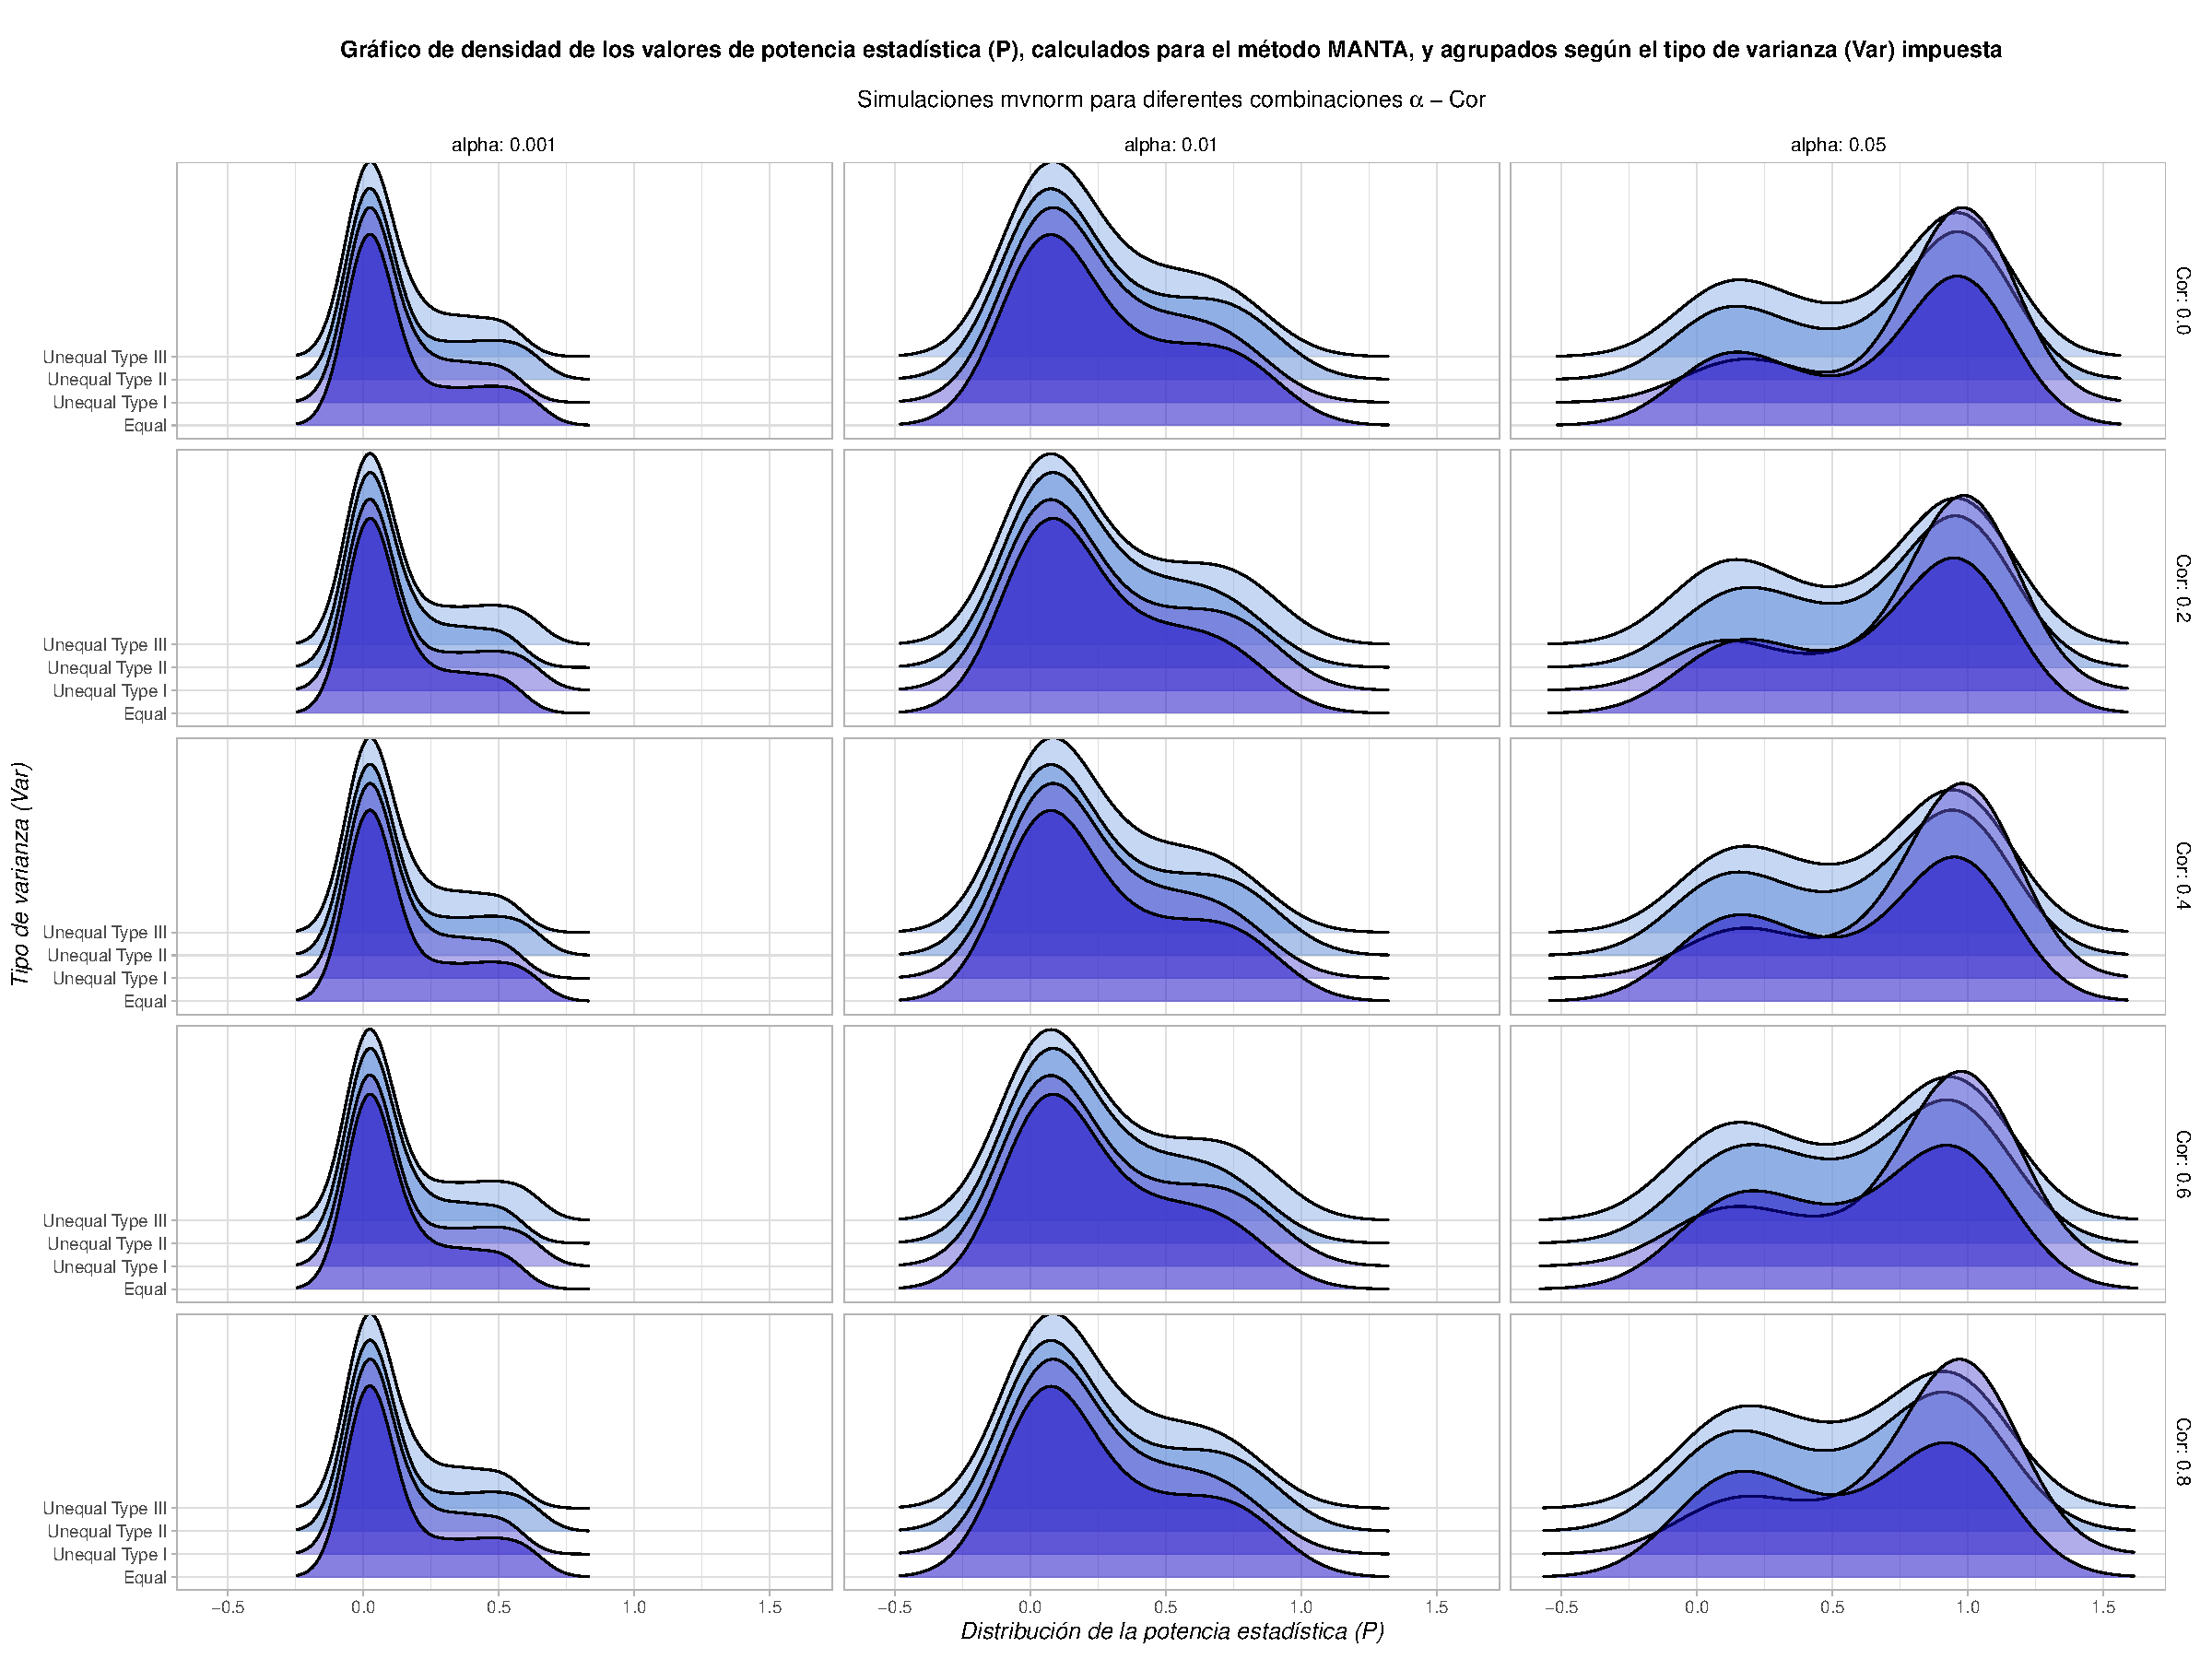
\includegraphics[width = \textwidth]{OBJ1mvnormStatsHomogMANTACorAlpha.pdf}
\caption{OBJ1mvnormStatsHomogMANTACorAlpha}
\label{figAppend:OBJ1mvnormStatsHomogMANTACorAlpha}
\end{subfigure}
\begin{subfigure}{0.49\textwidth}
\centering
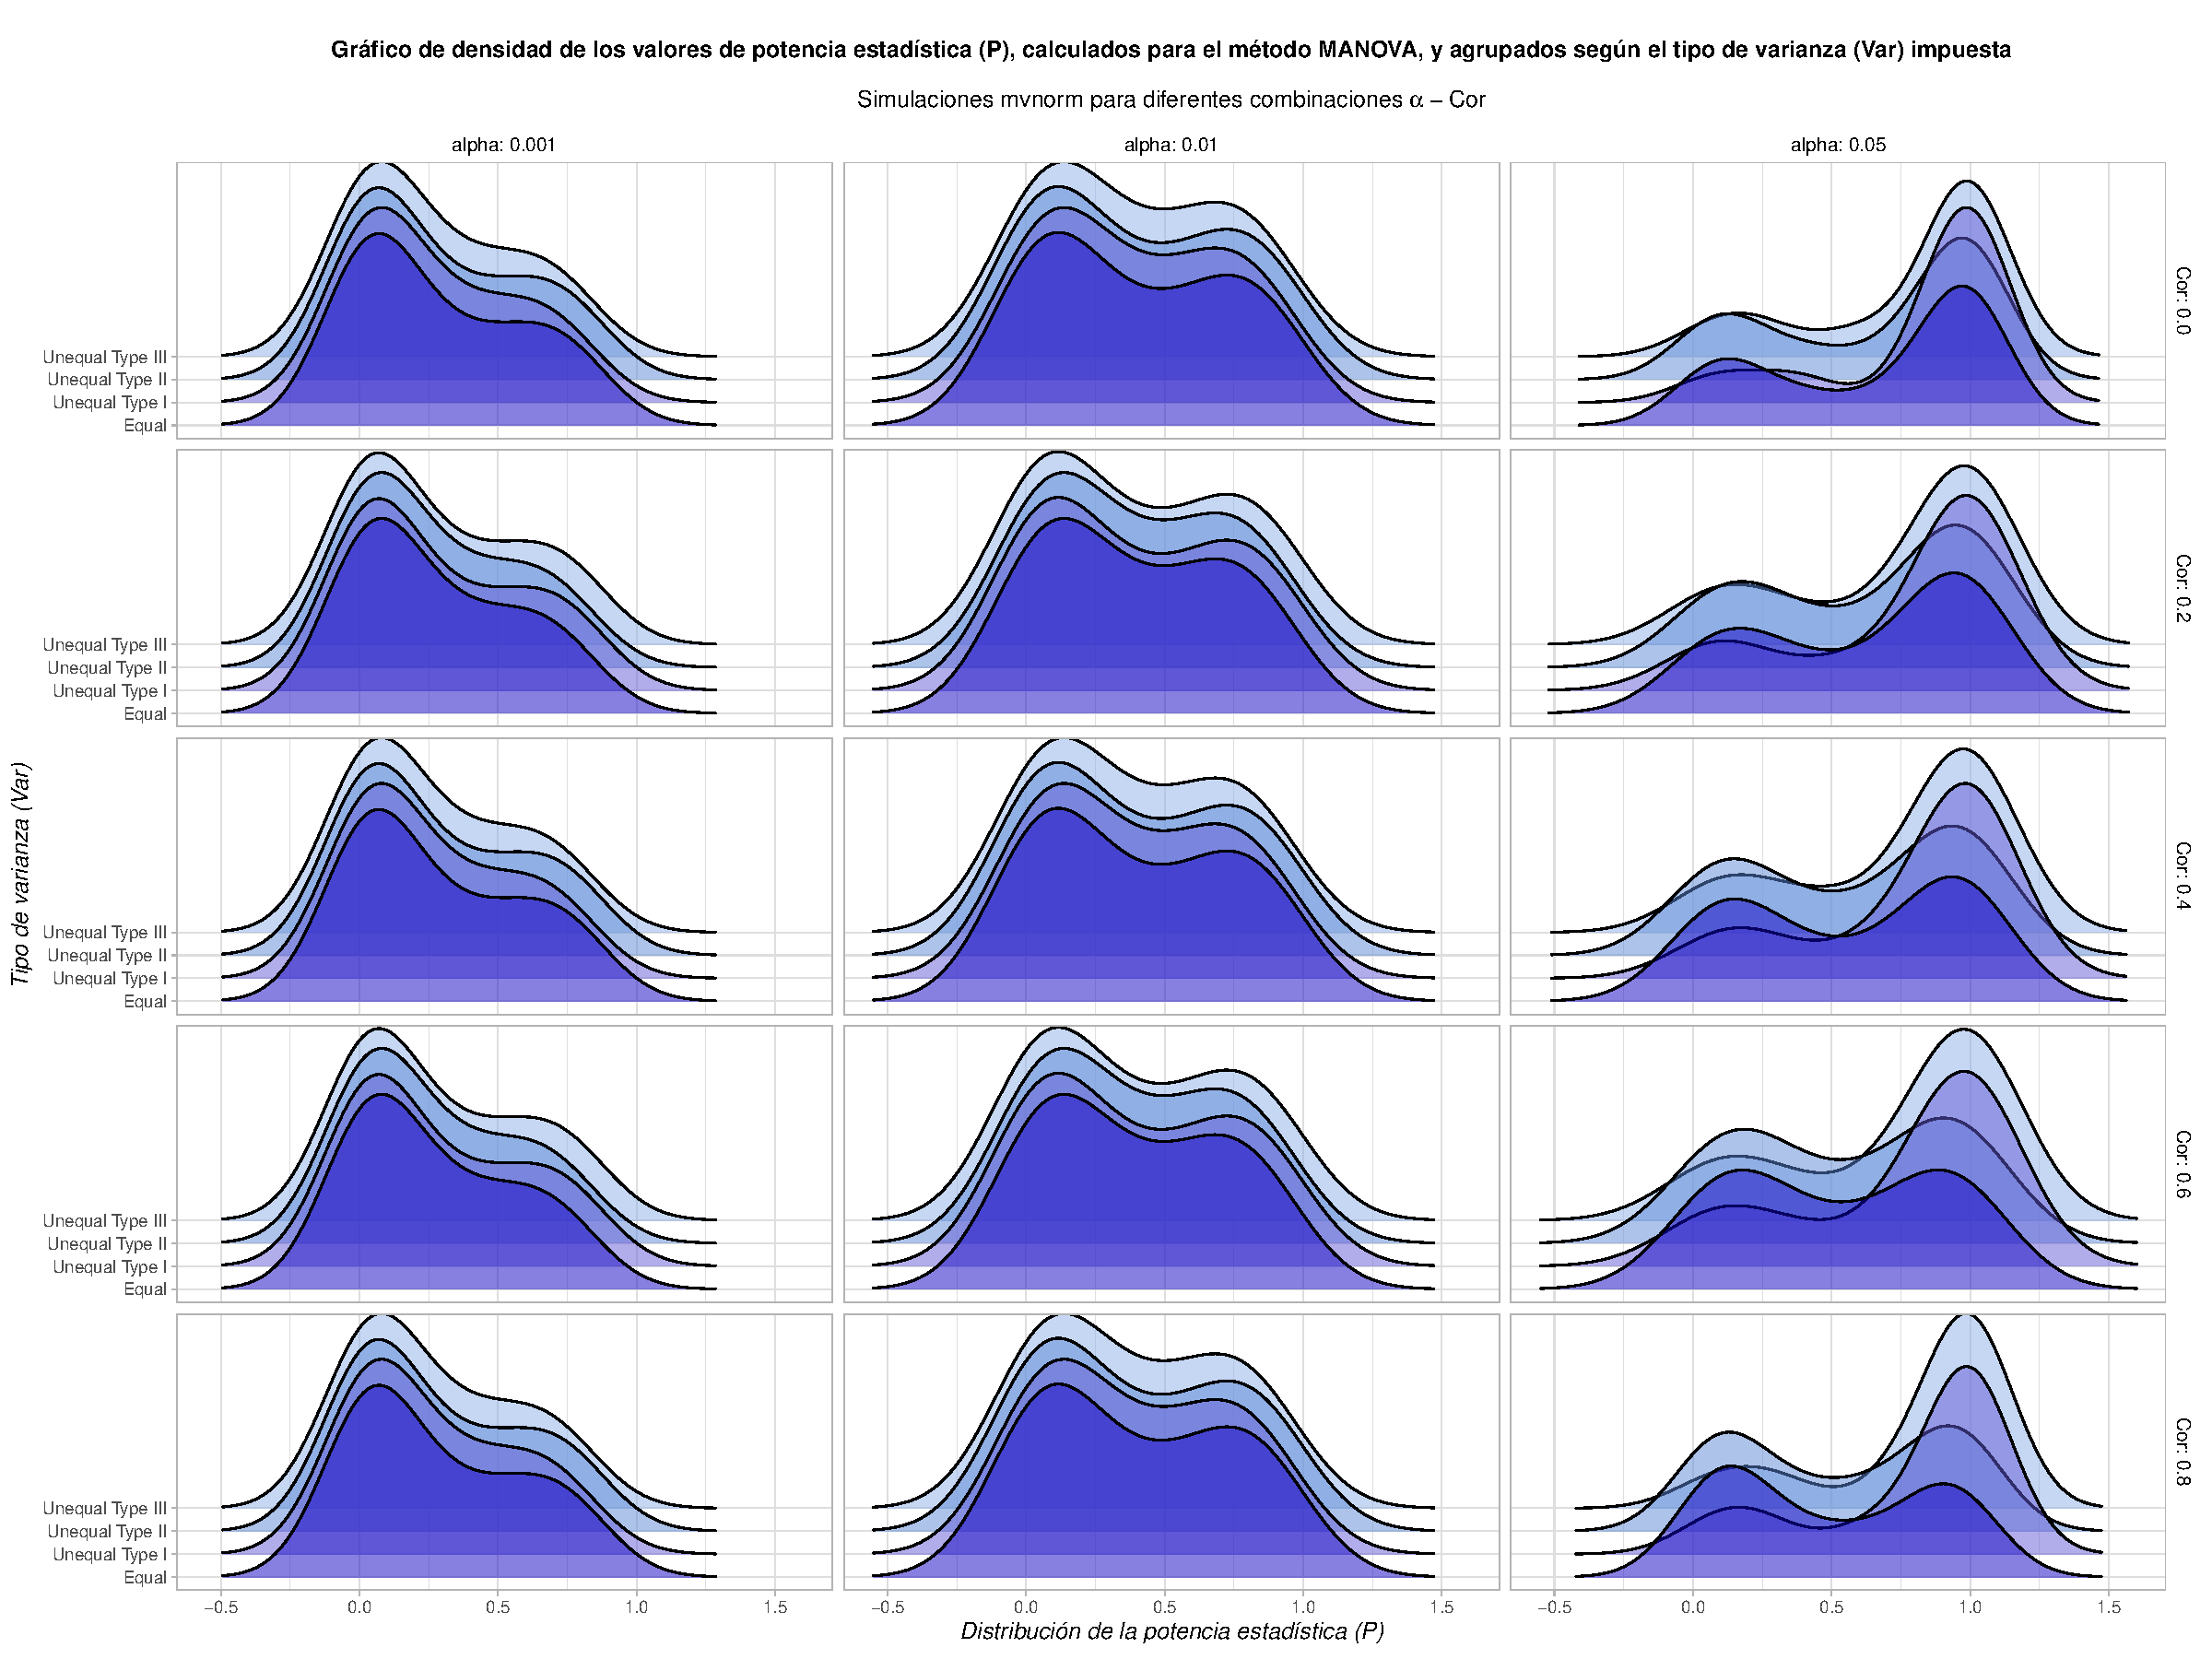
\includegraphics[width = \textwidth]{OBJ1mvnormStatsHomogMANOVACorAlpha.pdf}
\caption{OBJ1mvnormStatsHomogMANOVACorAlpha}
\label{figAppend:OBJ1mvnormStatsHomogMANOVACorAlpha}
\end{subfigure}
\\
\begin{subfigure}{0.49\textwidth}
\centering
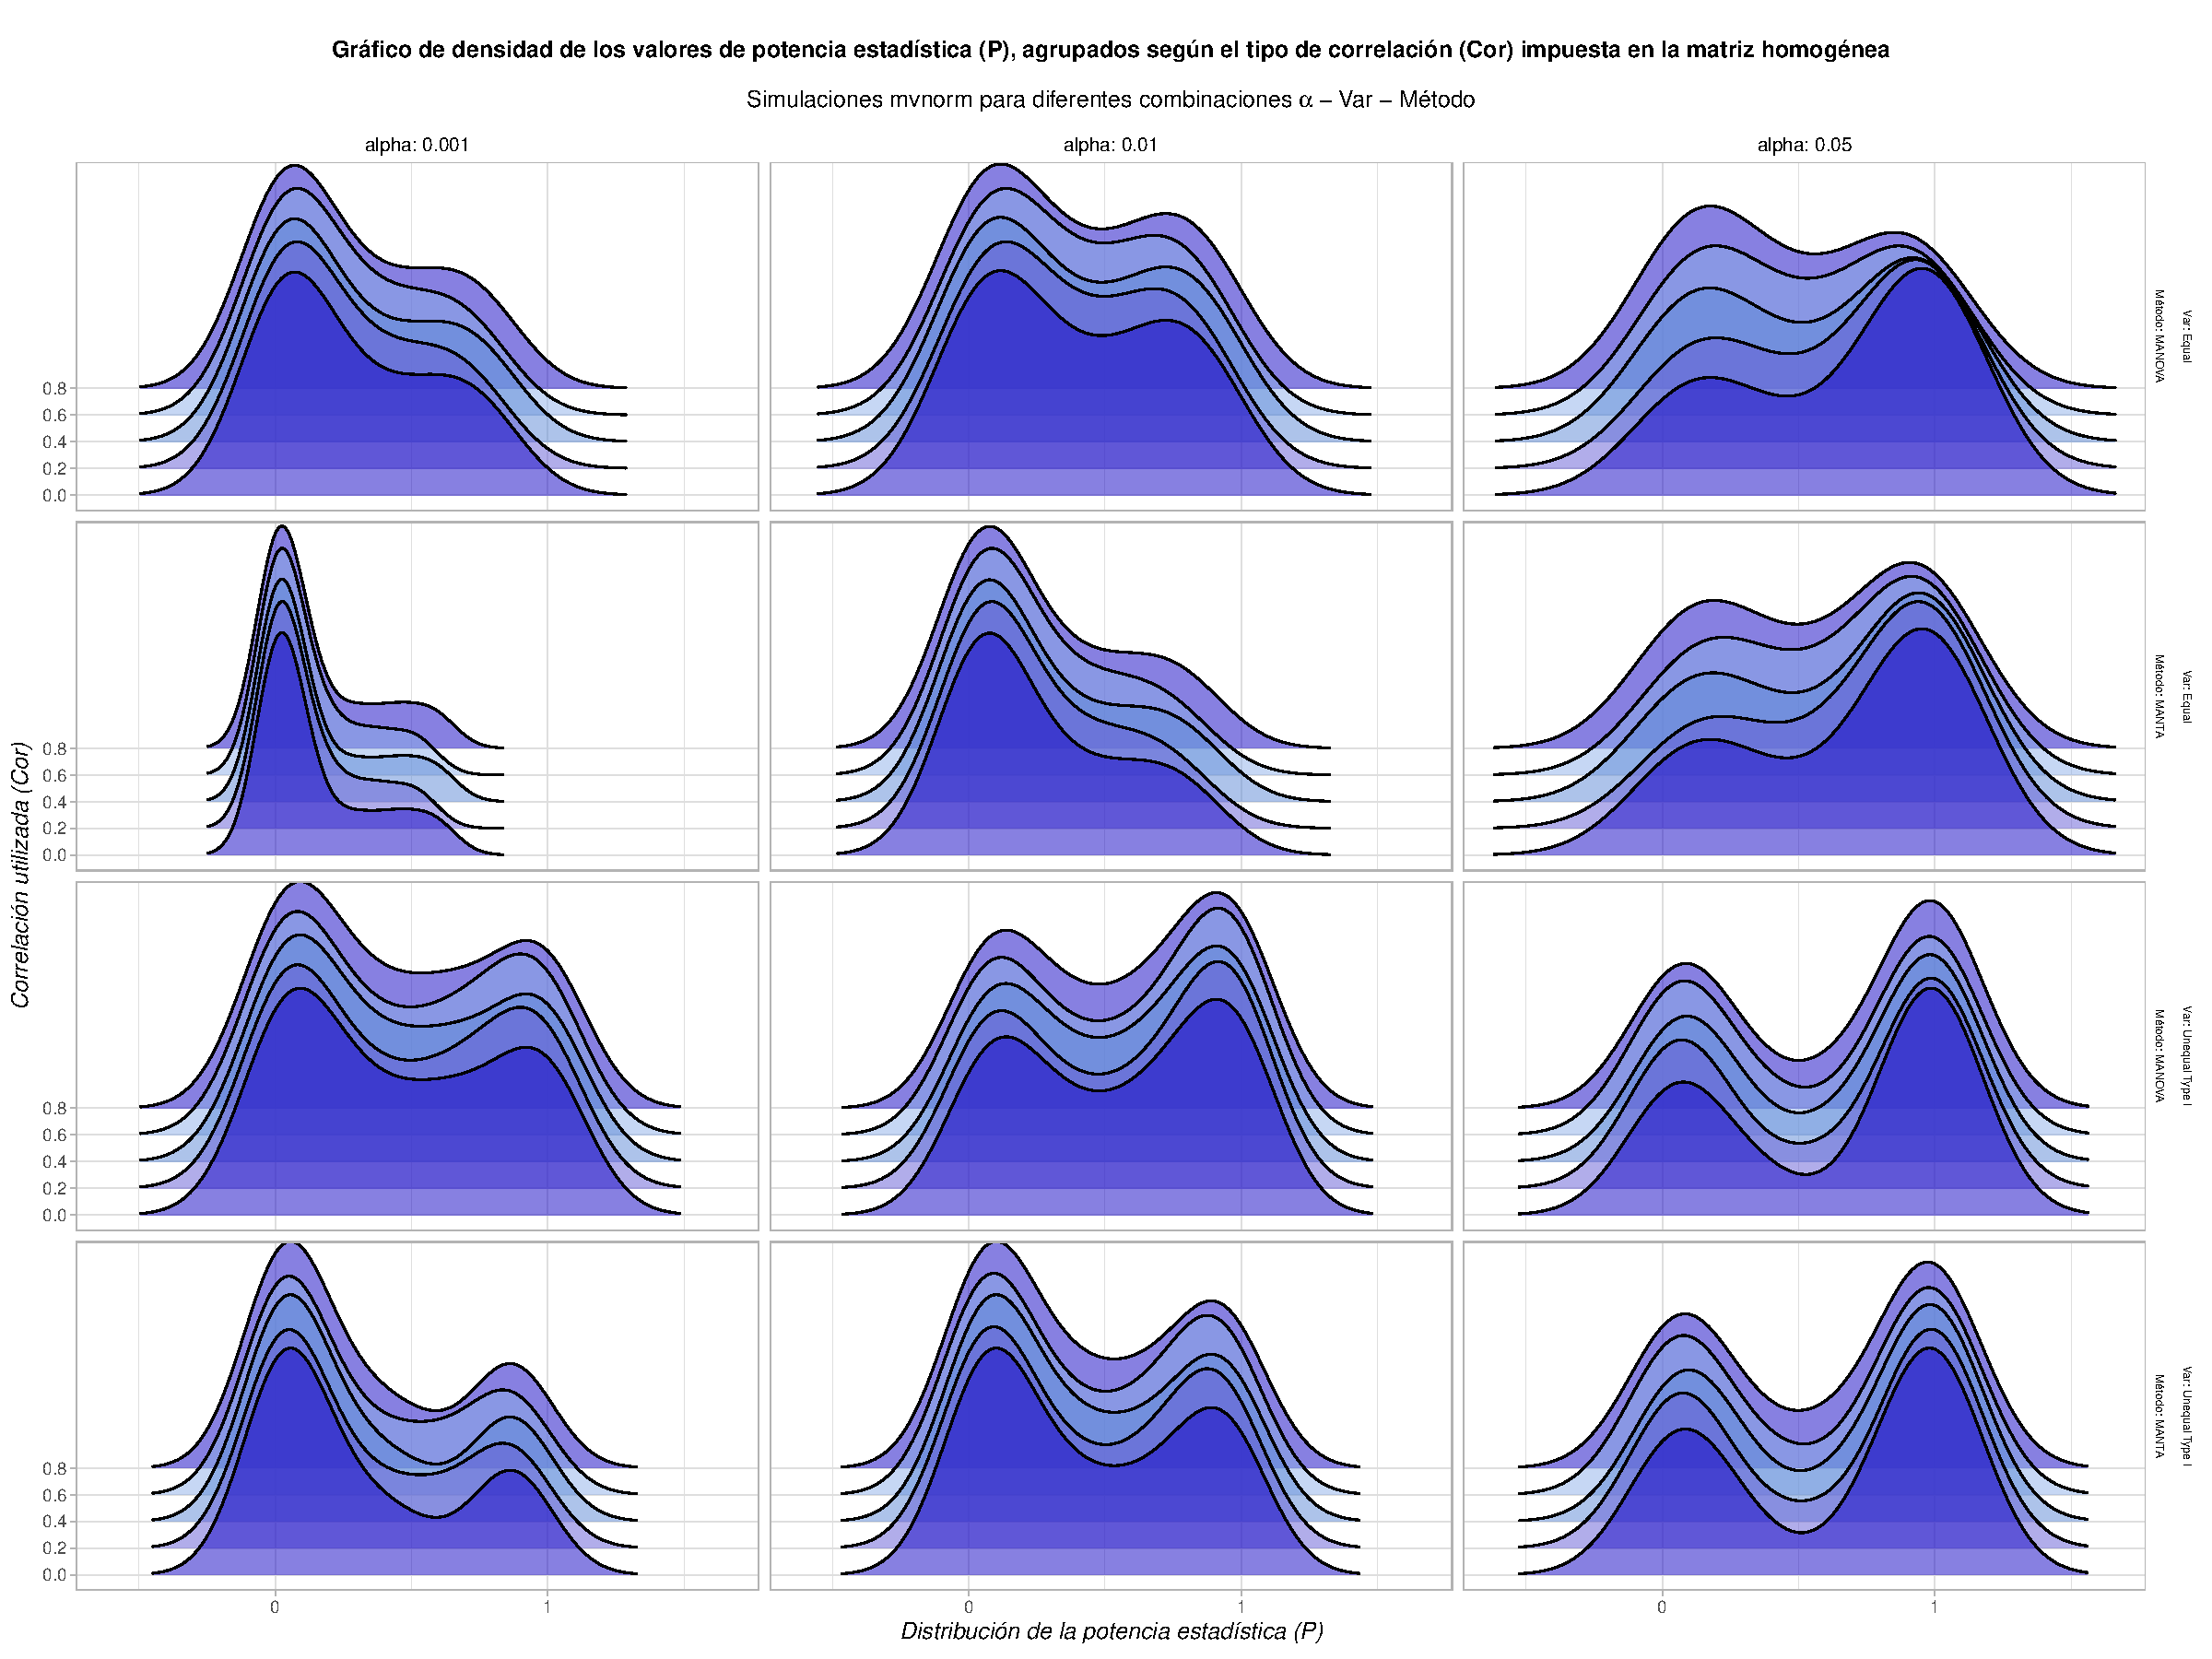
\includegraphics[width = \textwidth]{OBJ1mvnormStatsHomogMANTAMANOVAVar1.pdf}
\caption{OBJ1mvnormStatsHomogMANTAMANOVAVar1}
\label{figAppend:OBJ1mvnormStatsHomogMANTAMANOVAVar1}
\end{subfigure}
\begin{subfigure}{0.49\textwidth}
\centering
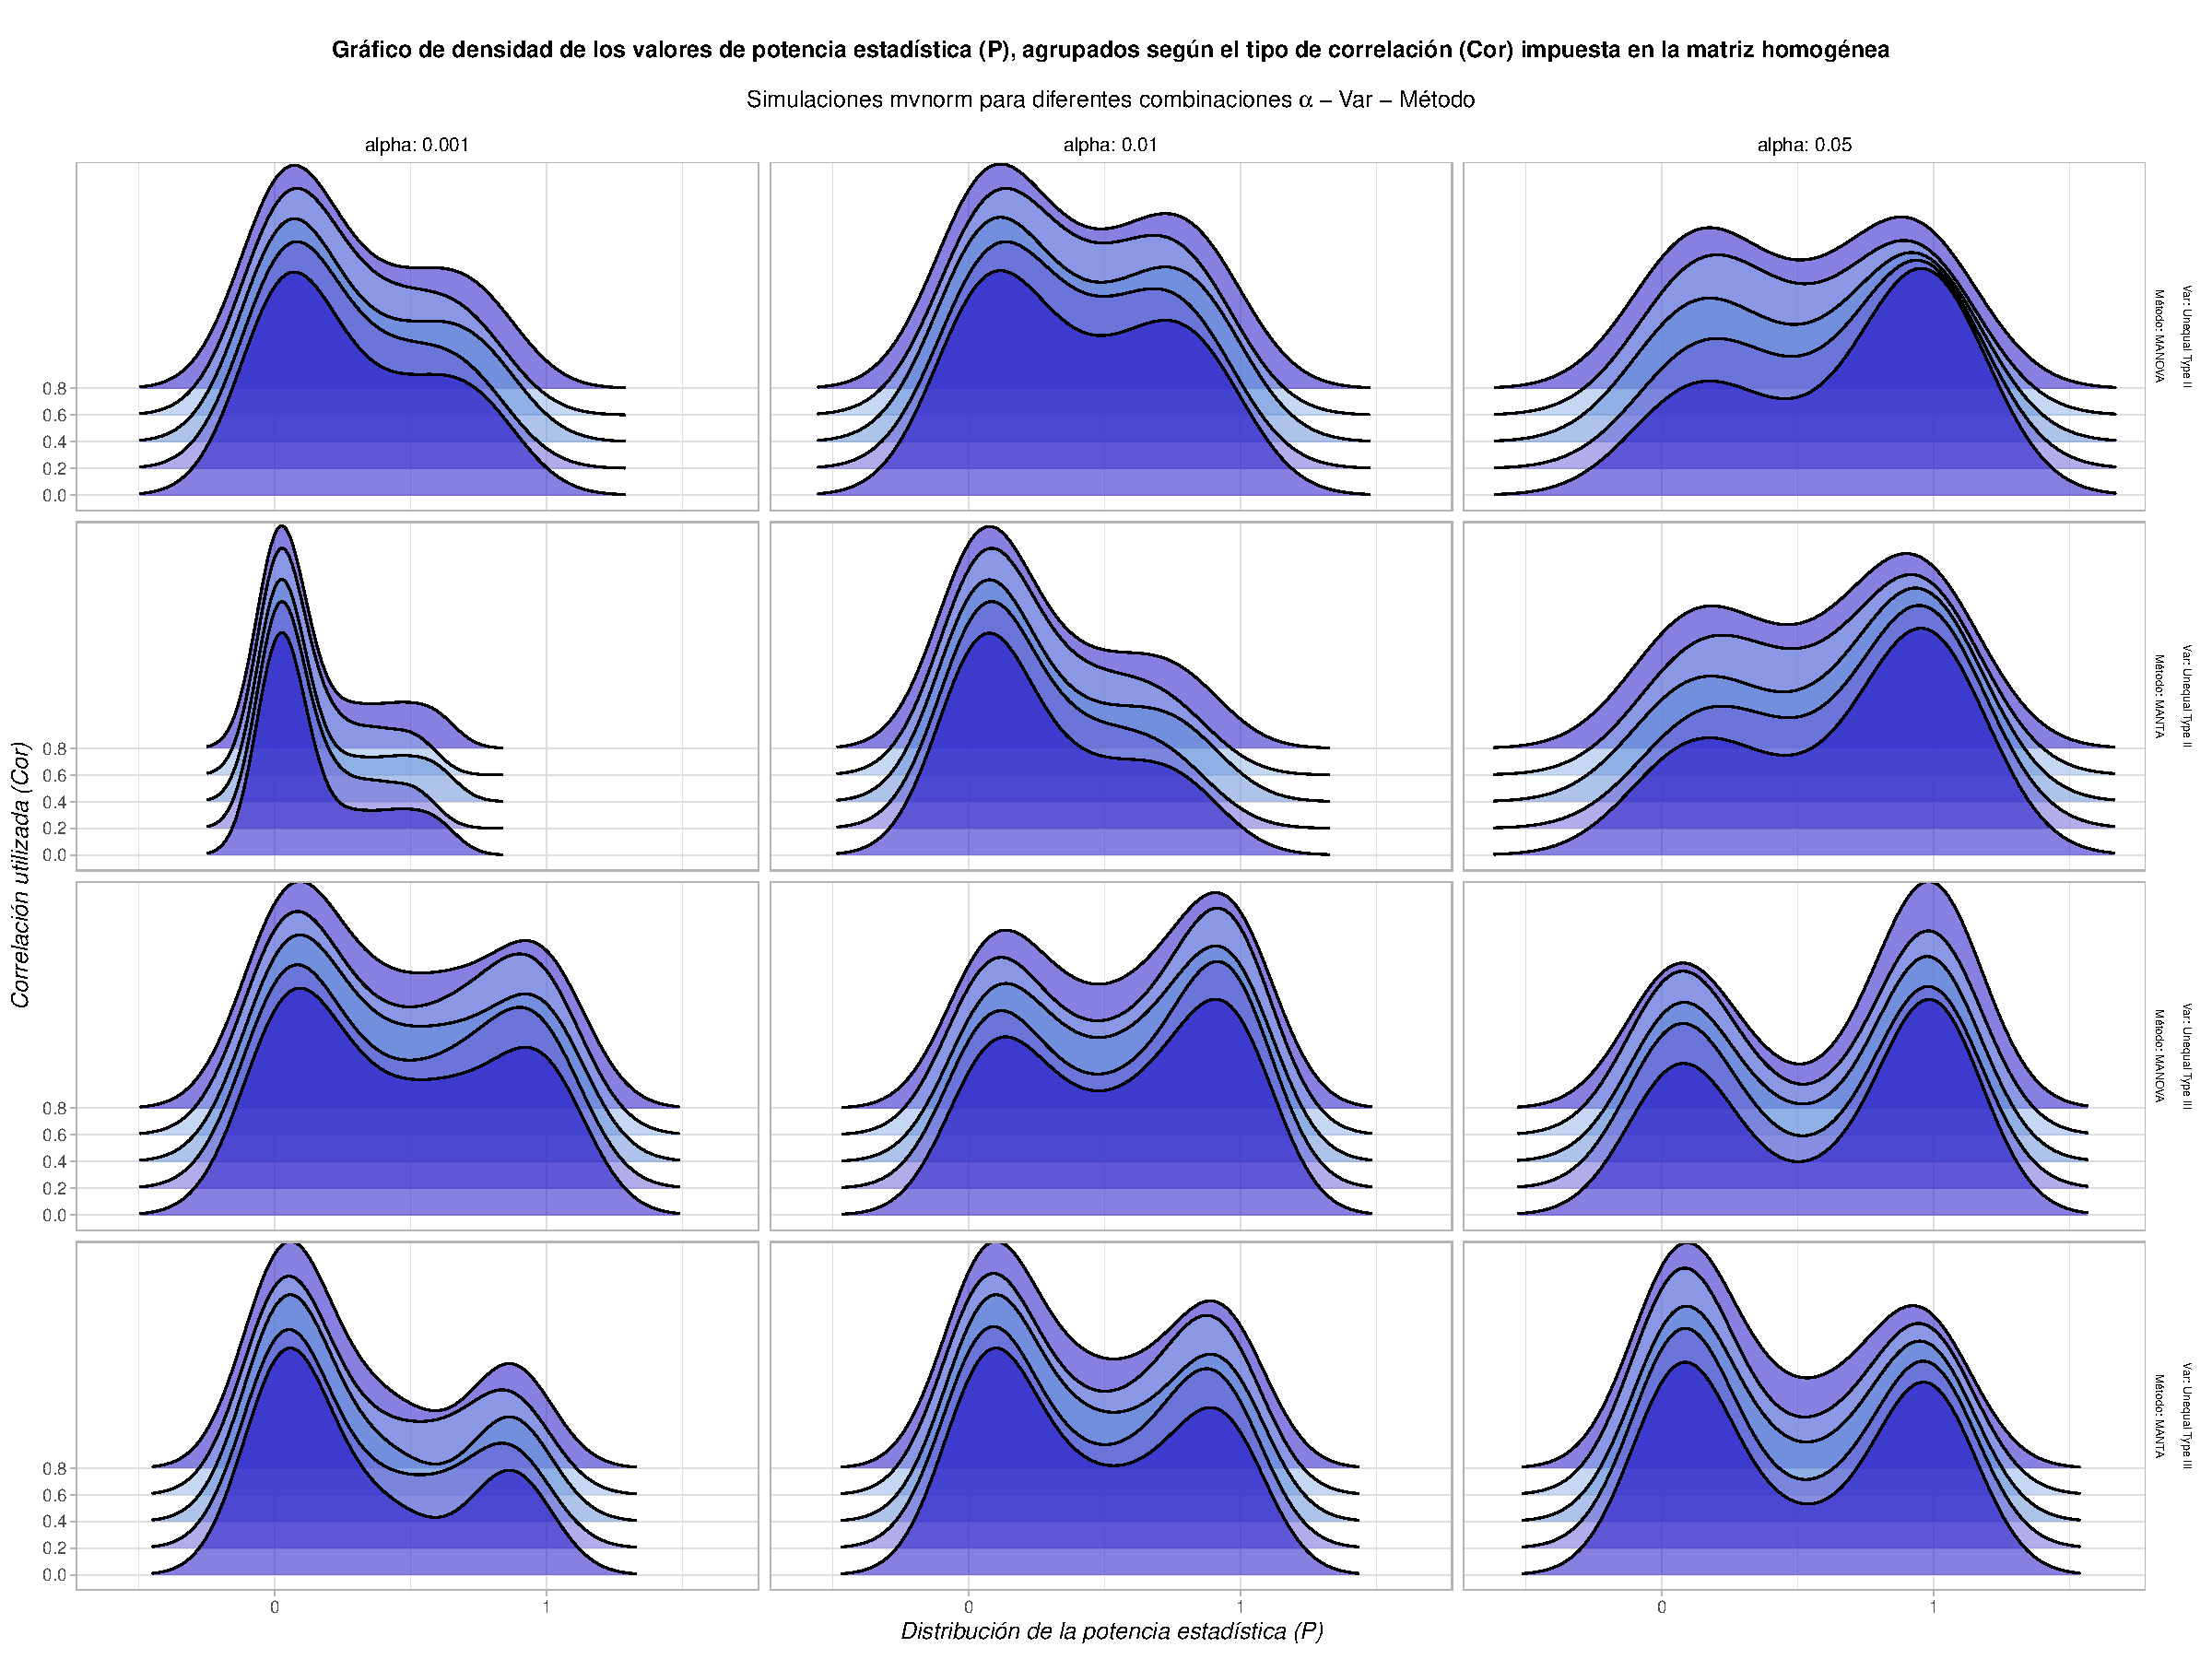
\includegraphics[width = \textwidth]{OBJ1mvnormStatsHomogMANTAMANOVAVar2.pdf}
\caption{OBJ1mvnormStatsHomogMANTAMANOVAVar2}
\label{figAppend:OBJ1mvnormStatsHomogMANTAMANOVAVar2}
\end{subfigure}
\caption{OBJ1mvnormStatsHomog}
\label{figAppend:combined}
\end{figure}

% OBJ1mvnormStatsNoHomog.pdf 
\begin{figure}[!htbp]
\hspace*{-2.1cm} % Movimiento relativo del gráfico
    \centering
    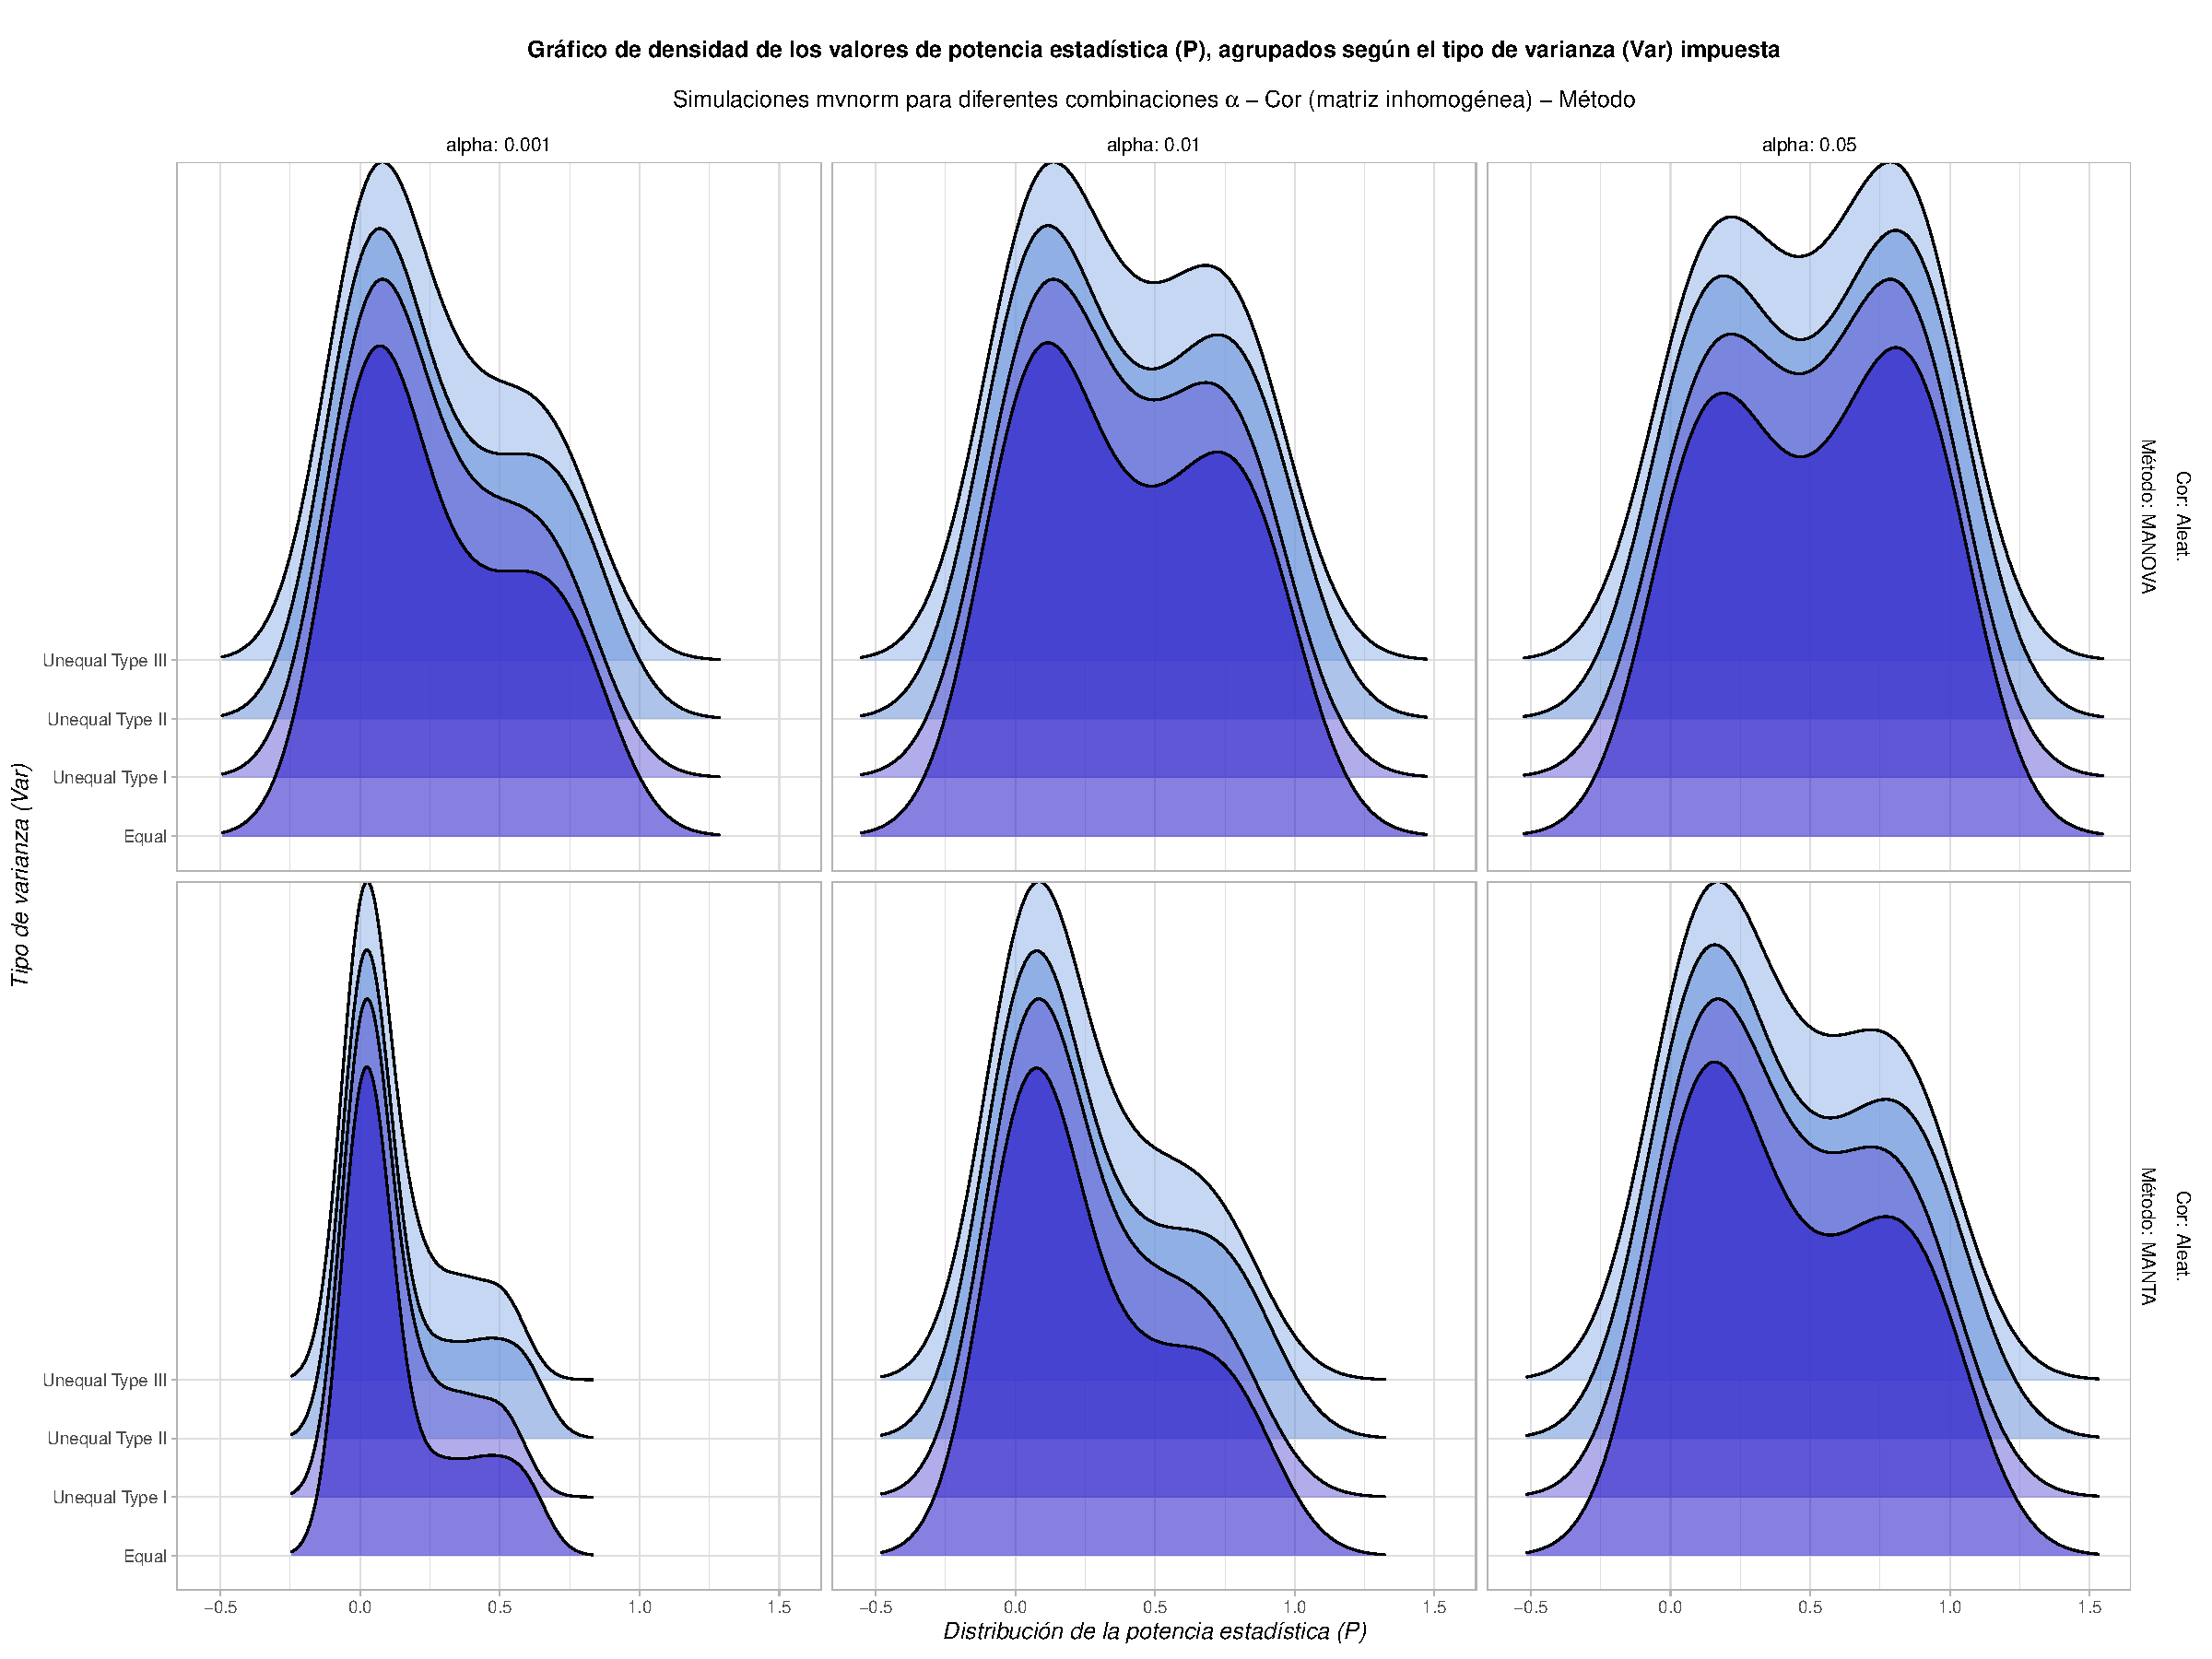
\includegraphics[scale=.3]{OBJ1mvnormStatsNoHomog.pdf}
    \caption{\scriptsize{A.}}
    \label{figAppend:OBJ1mvnormStatsNoHomog}
\end{figure}

% OBJ1a005.pdf
\begin{figure}[!htbp]
% \hspace*{-1.6cm} % Movimiento relativo del gráfico
    \centering
    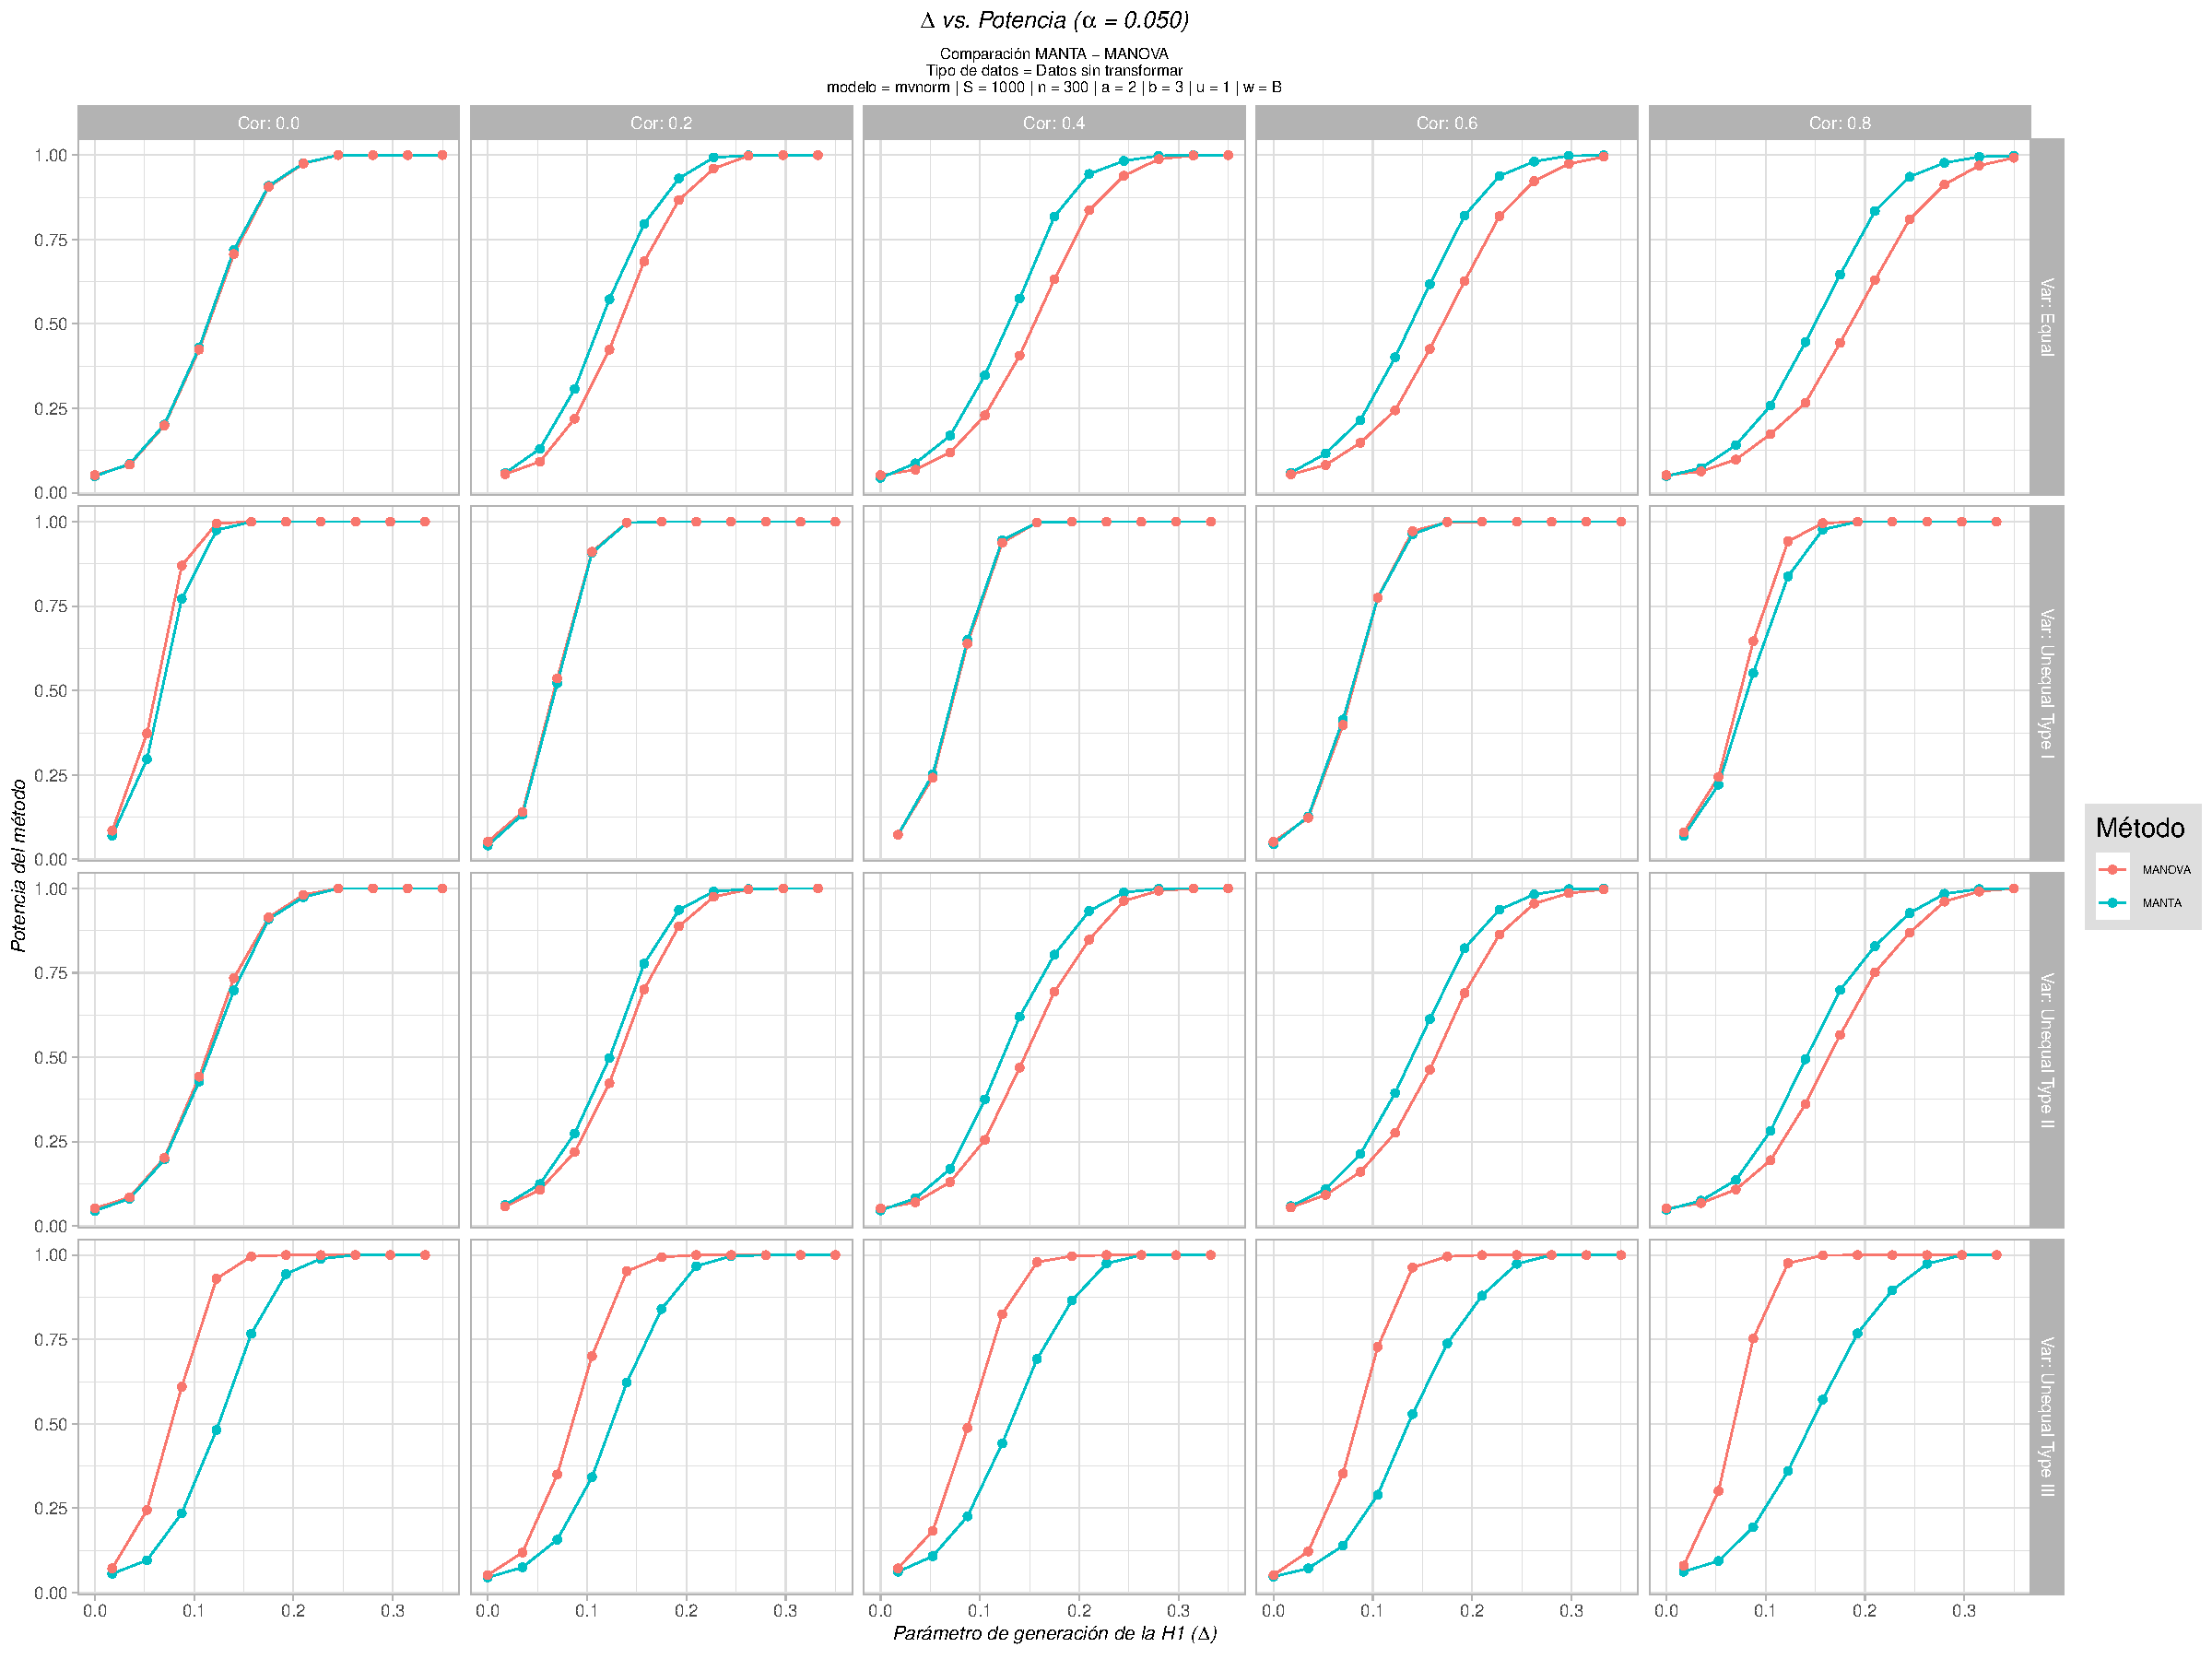
\includegraphics[scale=.45]{OBJ1a005.pdf}
    \caption{\scriptsize{A.}}
    \label{figAppend:OBJ1a005}
\end{figure}

% OBJ1bALEAT005.pdf
% OBJ1bALEATInvMANTAMANOVA001.pdf
% OBJ1bALEATInvMANTAMANOVA0001.pdf
% OBJ1bALEATInvMANTAMANOVA005.pdf
% OBJ1bHomclr001.pdf
% OBJ1bHomclr0001.pdf
% OBJ1bHomclr005.pdf
% OBJ1bHomInvMANOVA001.pdf
% OBJ1bHomInvMANOVA0001.pdf
% OBJ1bHomInvMANOVA005.pdf
% OBJ1bHomInvMANTA001.pdf
% OBJ1bHomInvMANTA0001.pdf
% OBJ1bHomInvMANTA005.pdf
% OBJ1bHomlog001.pdf
% OBJ1bHomlog0001.pdf
% OBJ1bHomlog005.pdf
% OBJ1bHomNoTransf001.pdf
% OBJ1bHomNoTransf0001.pdf
% OBJ1bHomNoTransf005.pdf
% OBJ1bHomsqrt001.pdf
% OBJ1bHomsqrt0001.pdf
% OBJ1bHomsqrt005.pdf
\begin{figure}[!htbp]
\hspace*{-1.6cm} % Movimiento relativo del gráfico
    \centering
    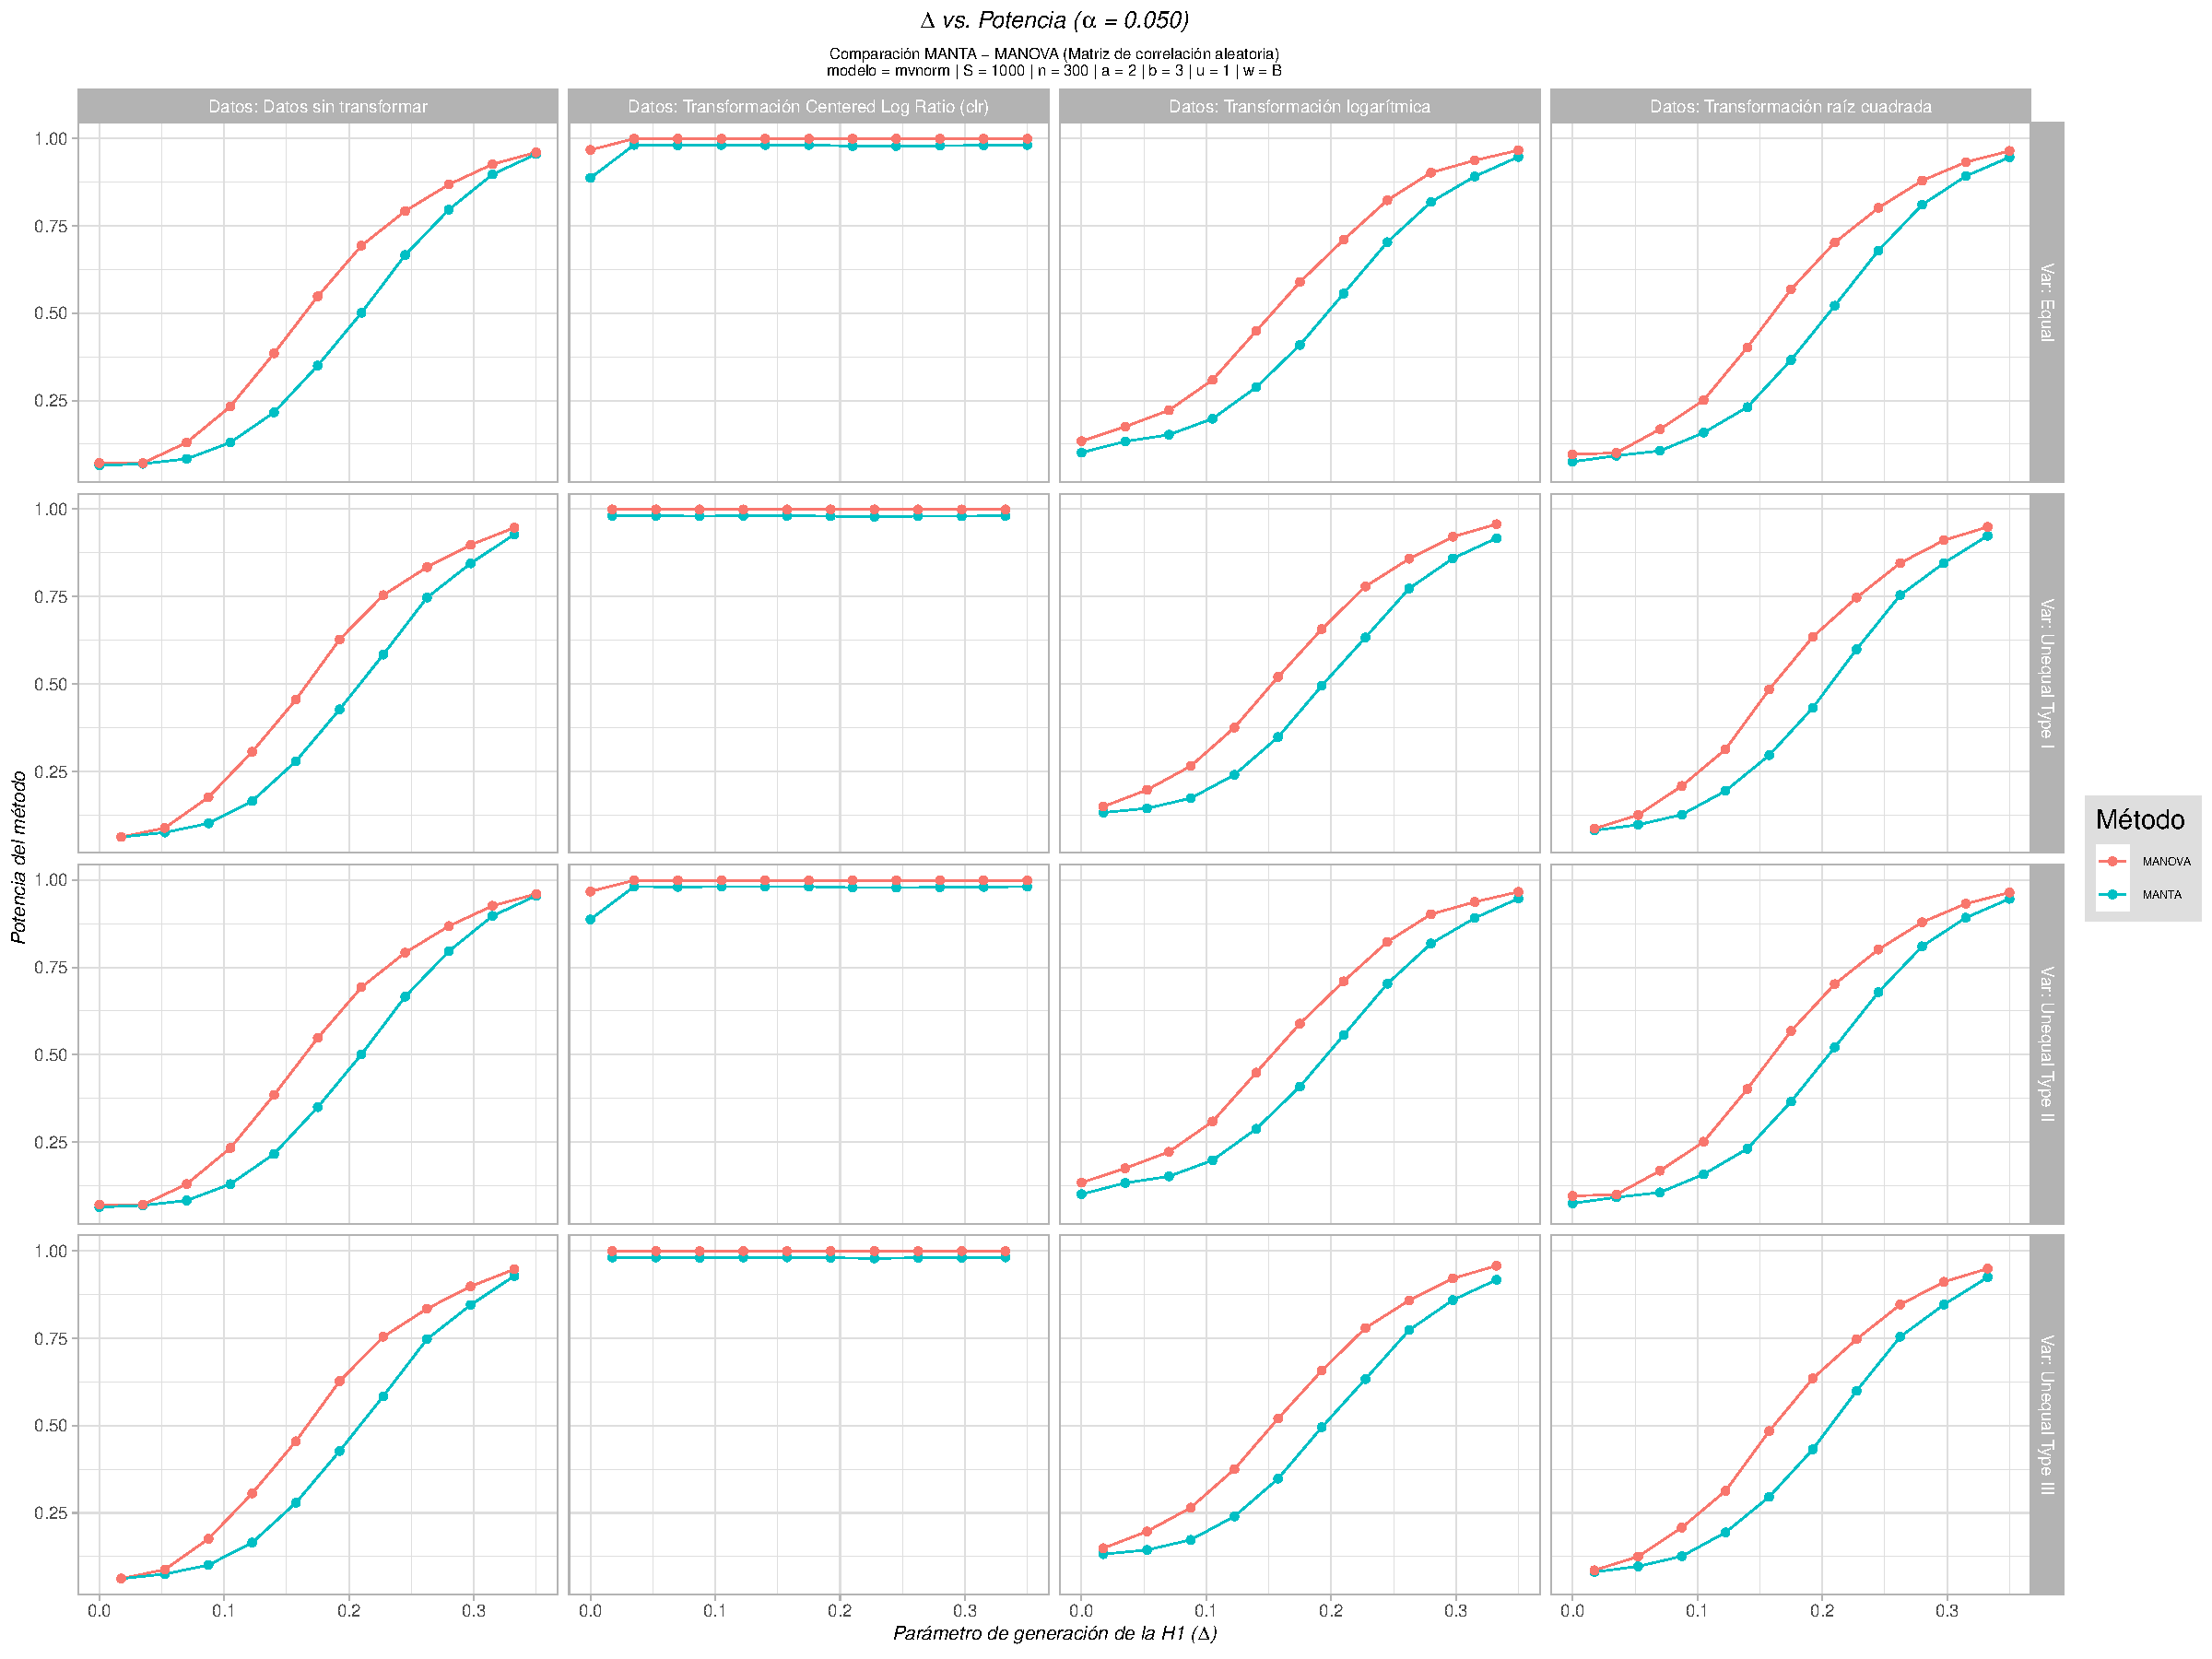
\includegraphics[scale=.51]{OBJ1bALEAT005.pdf}
    \caption{\scriptsize{A.}}
    \label{figAppend:OBJ1bALEAT005}
\end{figure}

% OBJ1c1005.pdf
% OBJ1c2001.pdf
% OBJ1c30001.pdf
\begin{figure}[!htbp]
\hspace*{-2cm} % Movimiento relativo del gráfico
\begin{subfigure}{.65\textwidth}
  \centering
  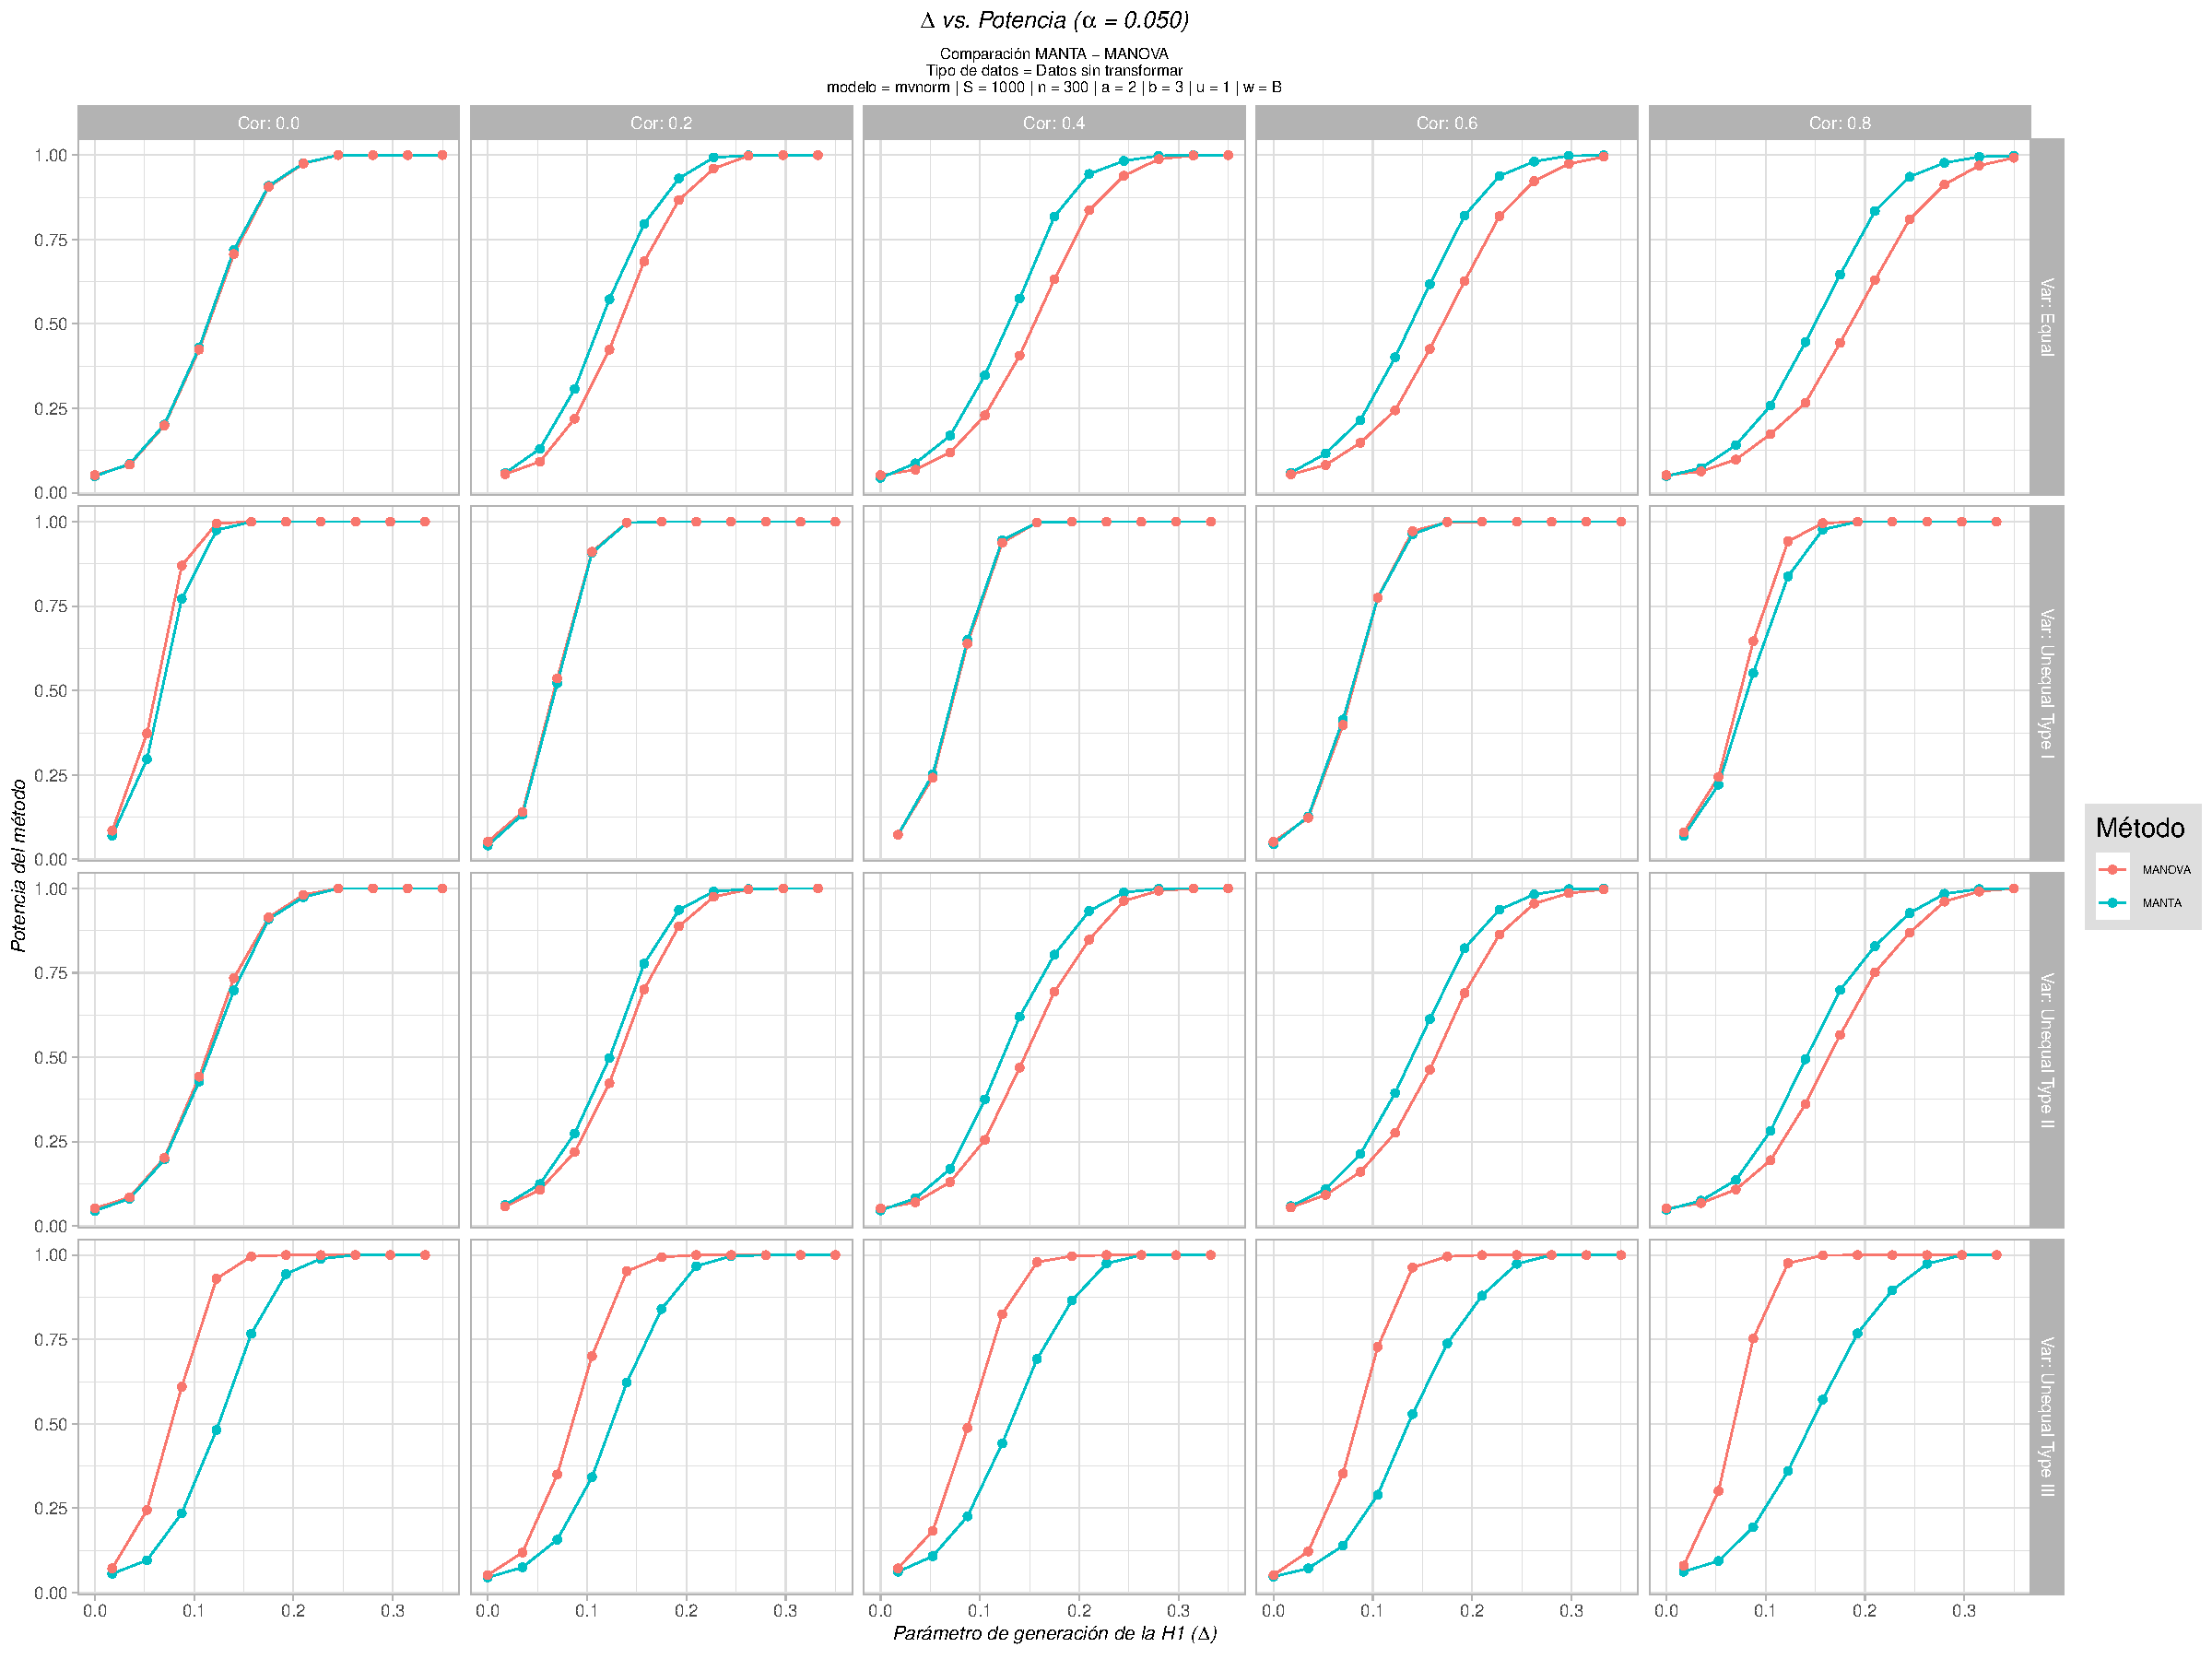
\includegraphics[width=.9\linewidth]{OBJ1c1005.pdf}
  \caption{\scriptsize{A.}}
  \label{figAppend:OBJ1c1005}
\end{subfigure}%
\begin{subfigure}{.65\textwidth}
\hspace*{-2.3cm} % Movimiento relativo del gráfico
  \centering
  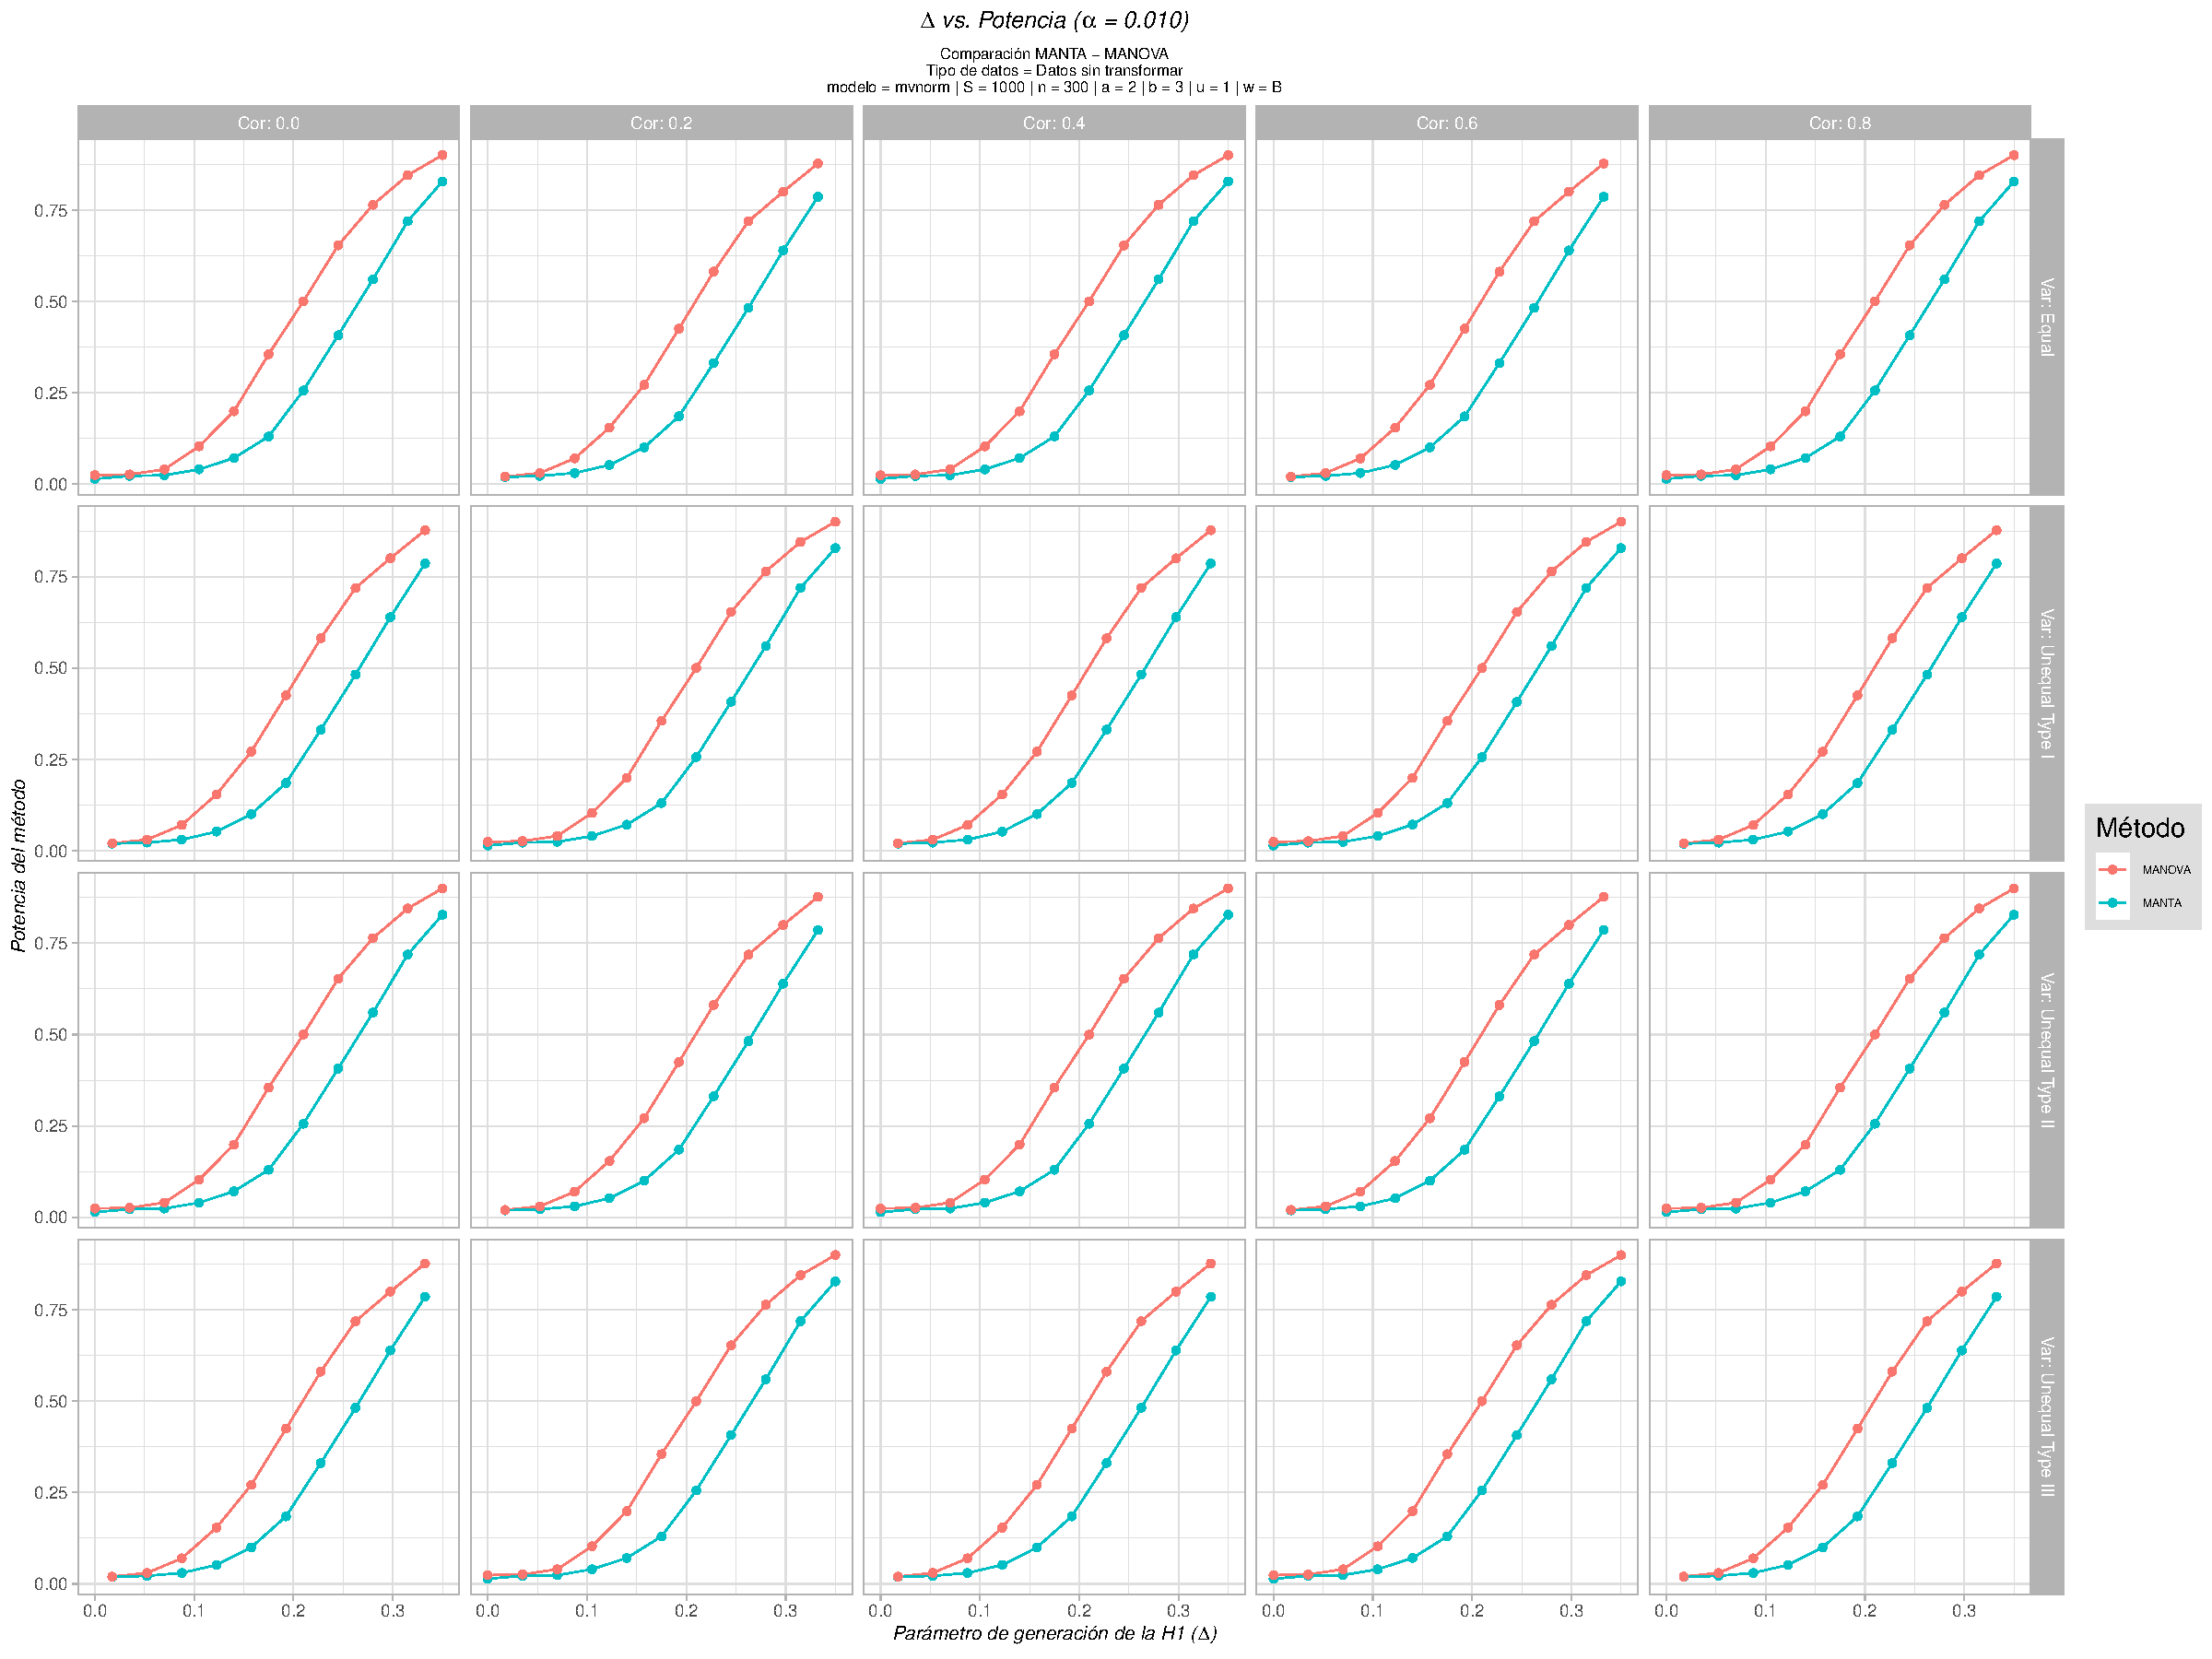
\includegraphics[width=.9\linewidth]{OBJ1c2001.pdf}
  \caption{\scriptsize{A.}}
  \label{figAppend:OBJ1c2001}
\end{subfigure}%
\\
\\
\begin{subfigure}{.65\textwidth}
\hspace*{3.5cm} % Movimiento relativo del gráfico
  \centering
  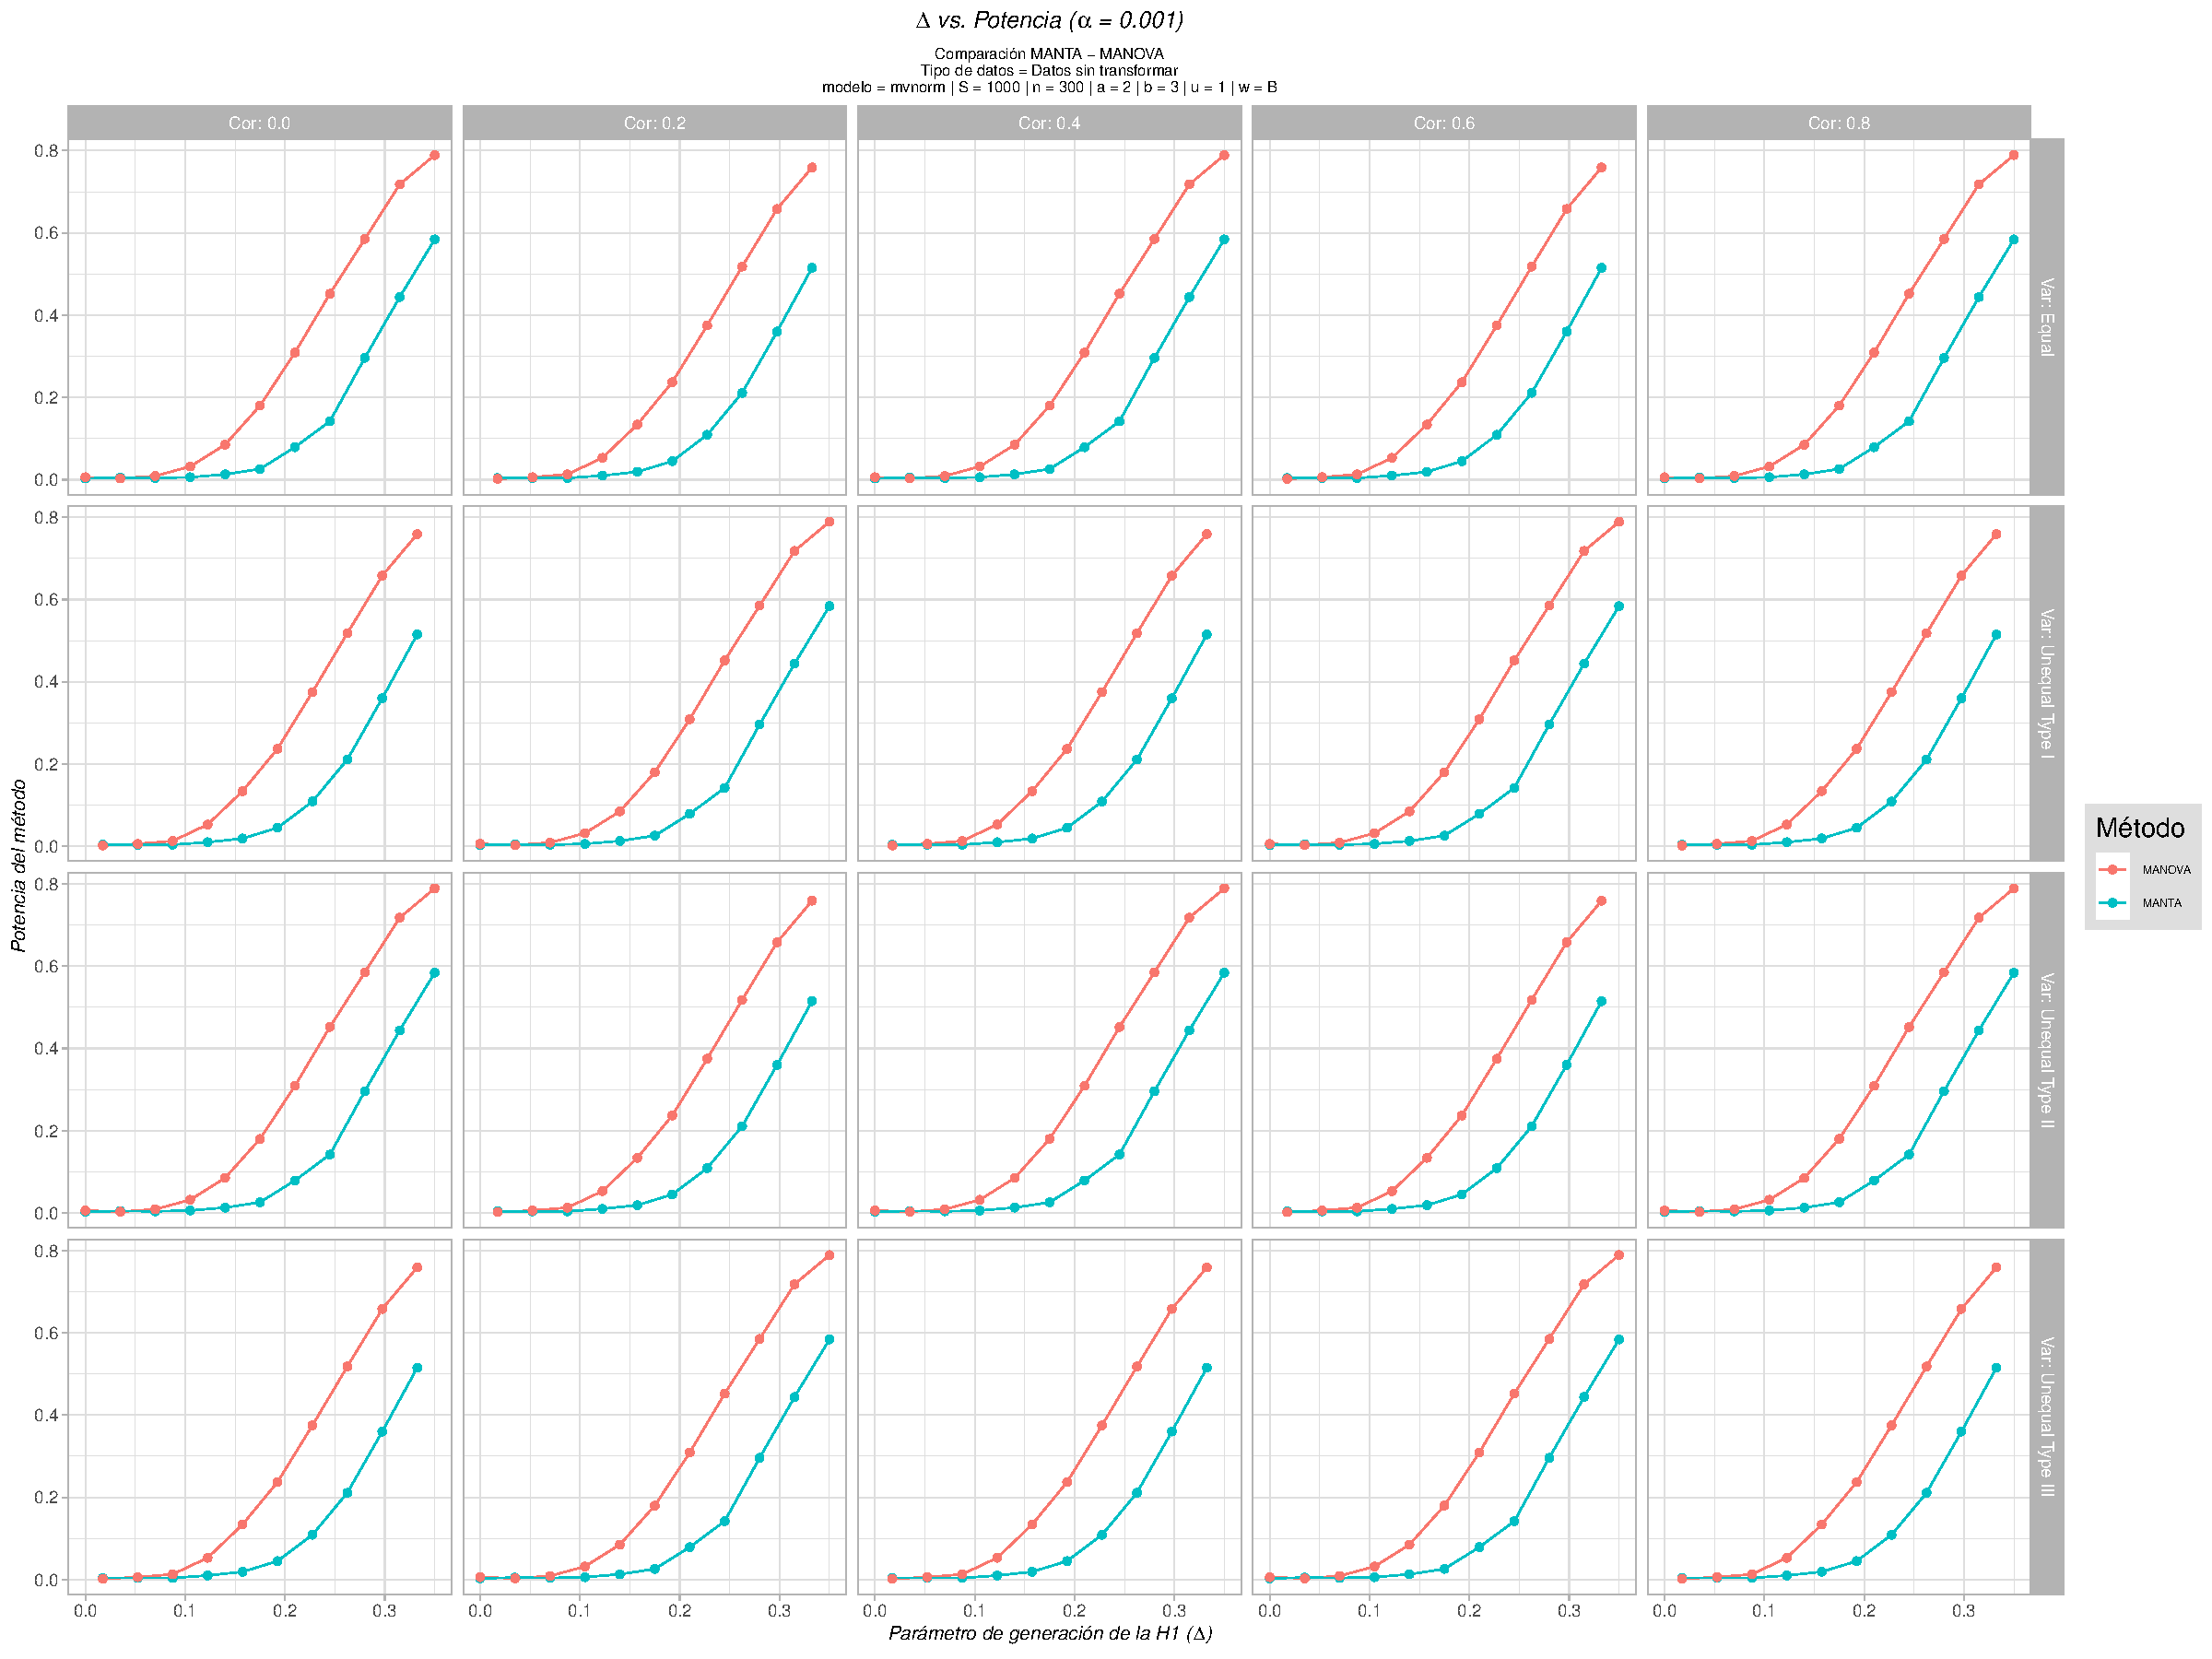
\includegraphics[width=.9\linewidth]{OBJ1c30001.pdf}
  \caption{\scriptsize{A.}}
  \label{figAppend:OBJ1c30001}
\end{subfigure}
\caption{\scriptsize{A.}}
\label{figAppend:OBJ1c}
\end{figure}

% OBJ1dallalpha.pdf
\begin{figure}[!htbp]
\hspace*{-1.6cm} % Movimiento relativo del gráfico
    \centering
    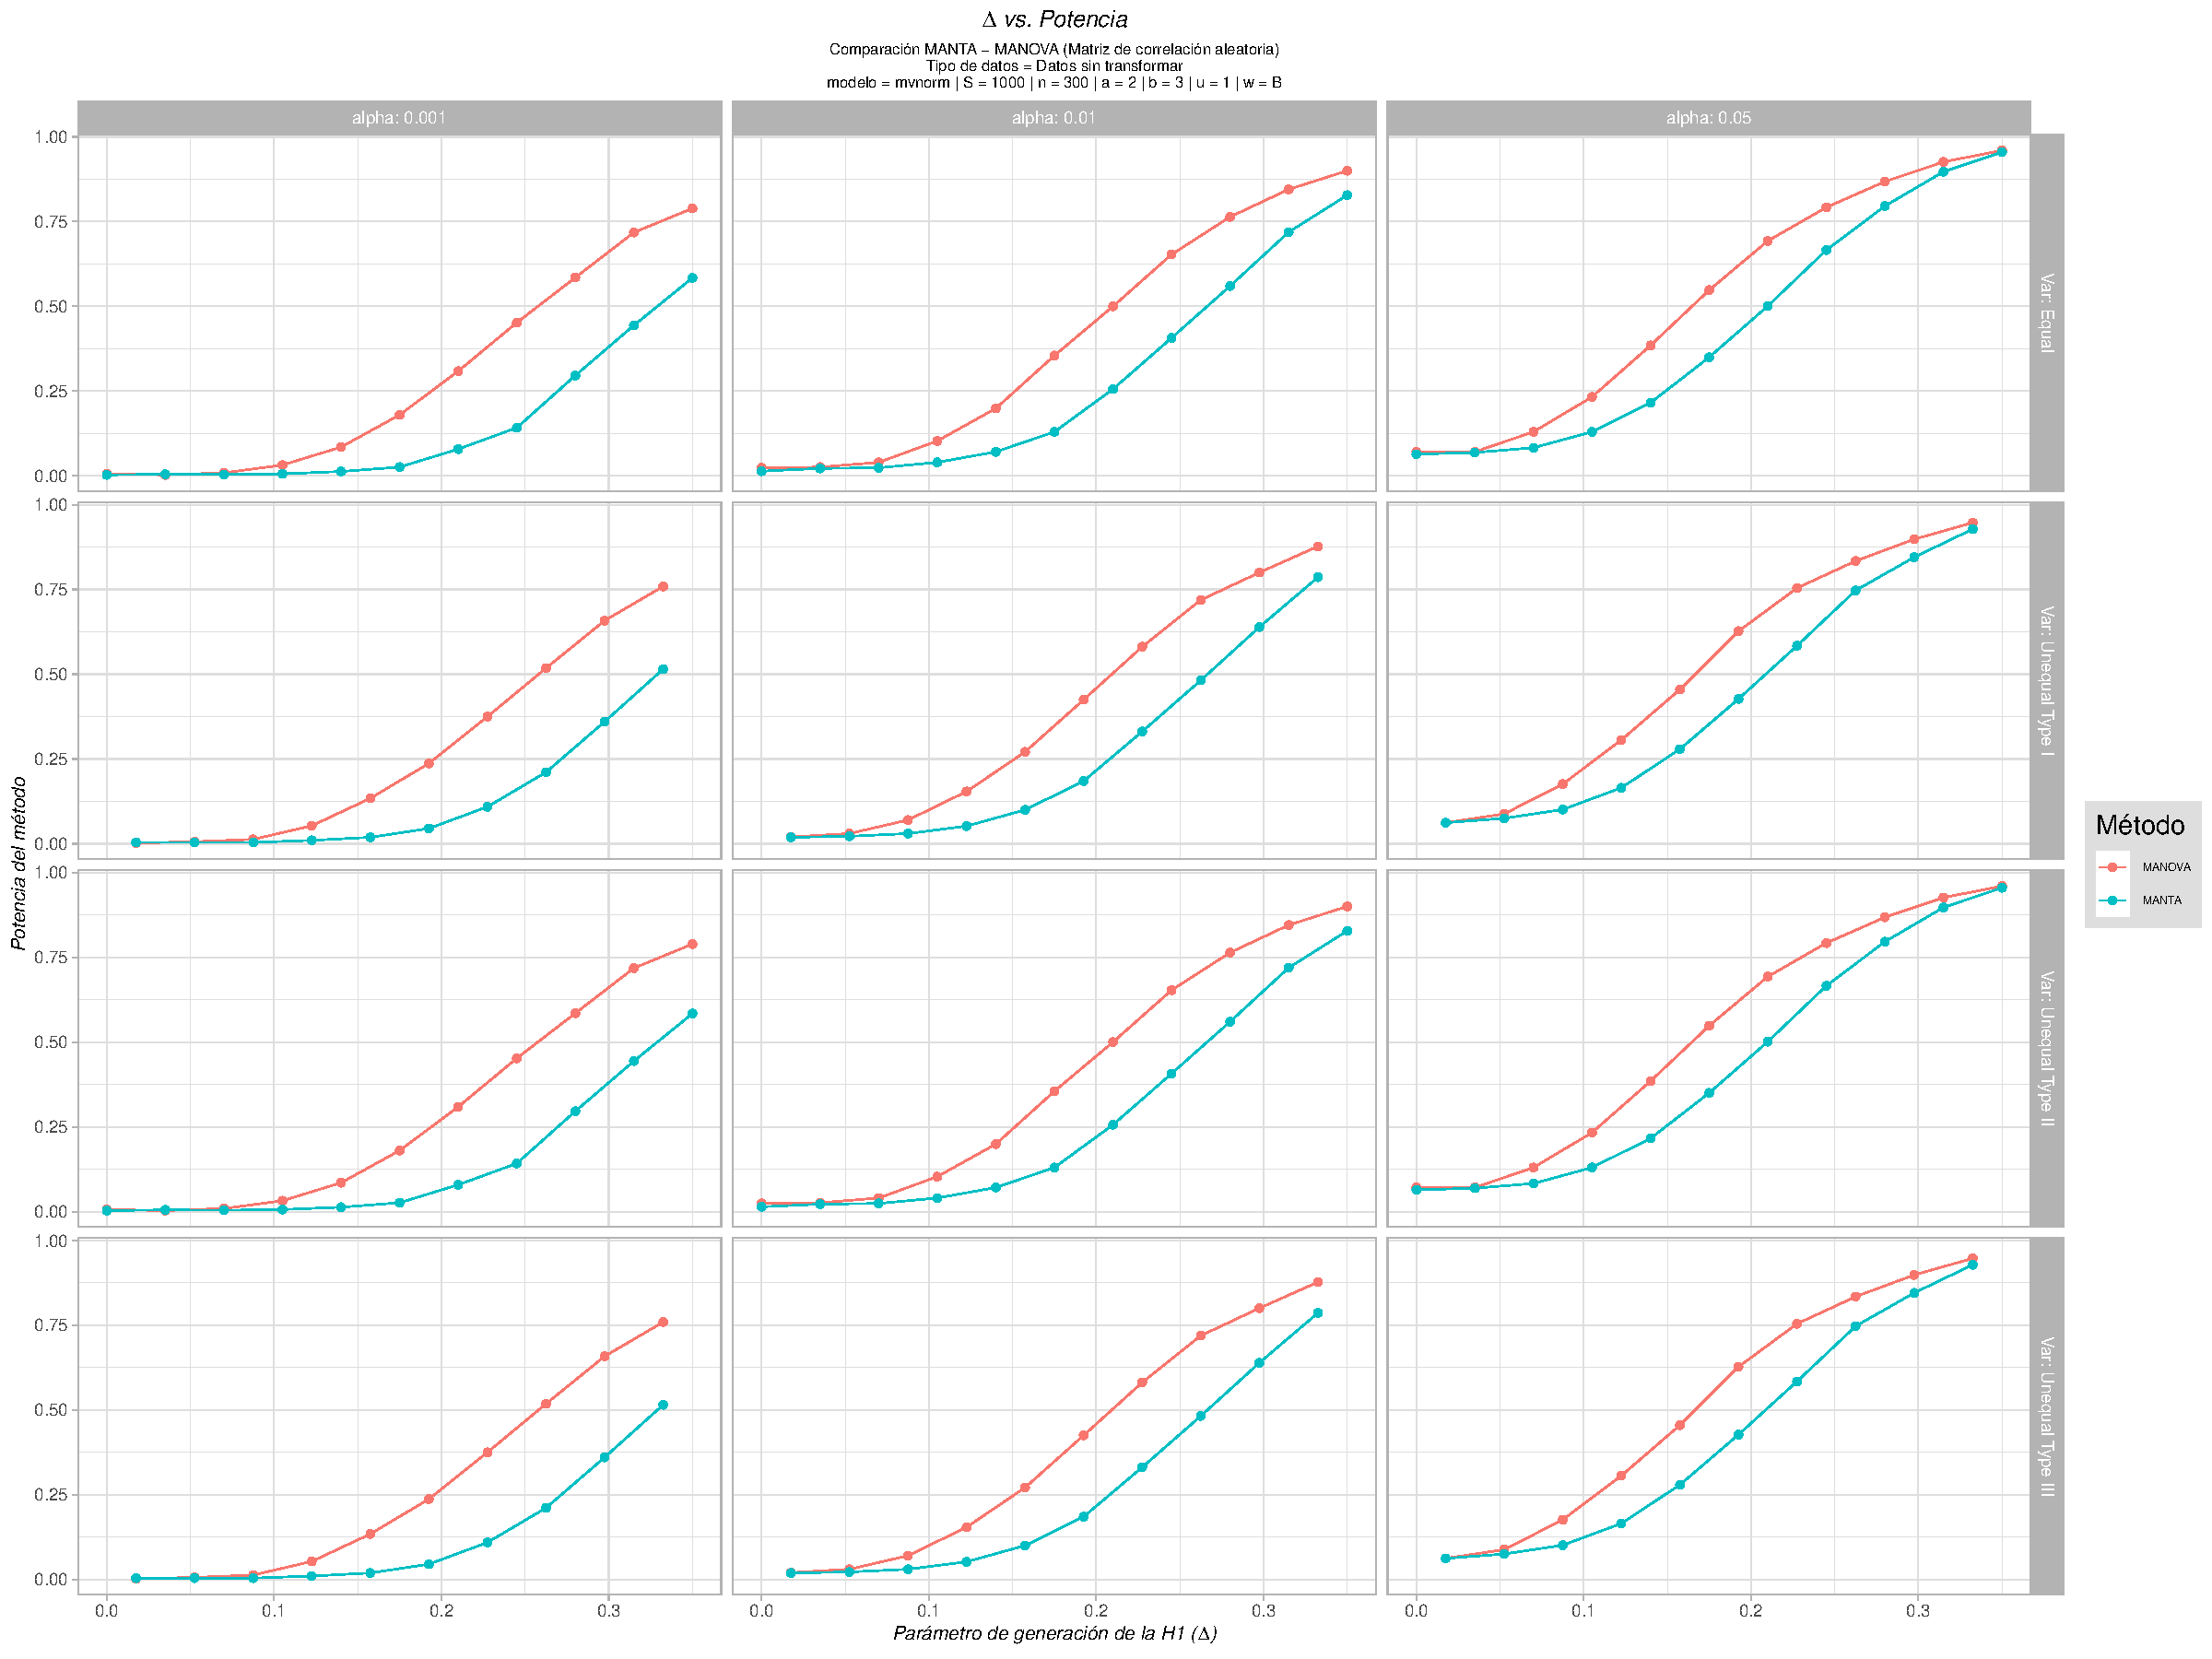
\includegraphics[scale=.51]{OBJ1dallalpha.pdf}
    \caption{\scriptsize{A.}}
    \label{figAppend:OBJ1dallalpha}
\end{figure}

%OBJ2SimplexStatswrapAlpha.pdf
\begin{figure}[!htbp]
\hspace*{-2.1cm} % Movimiento relativo del gráfico
    \centering
    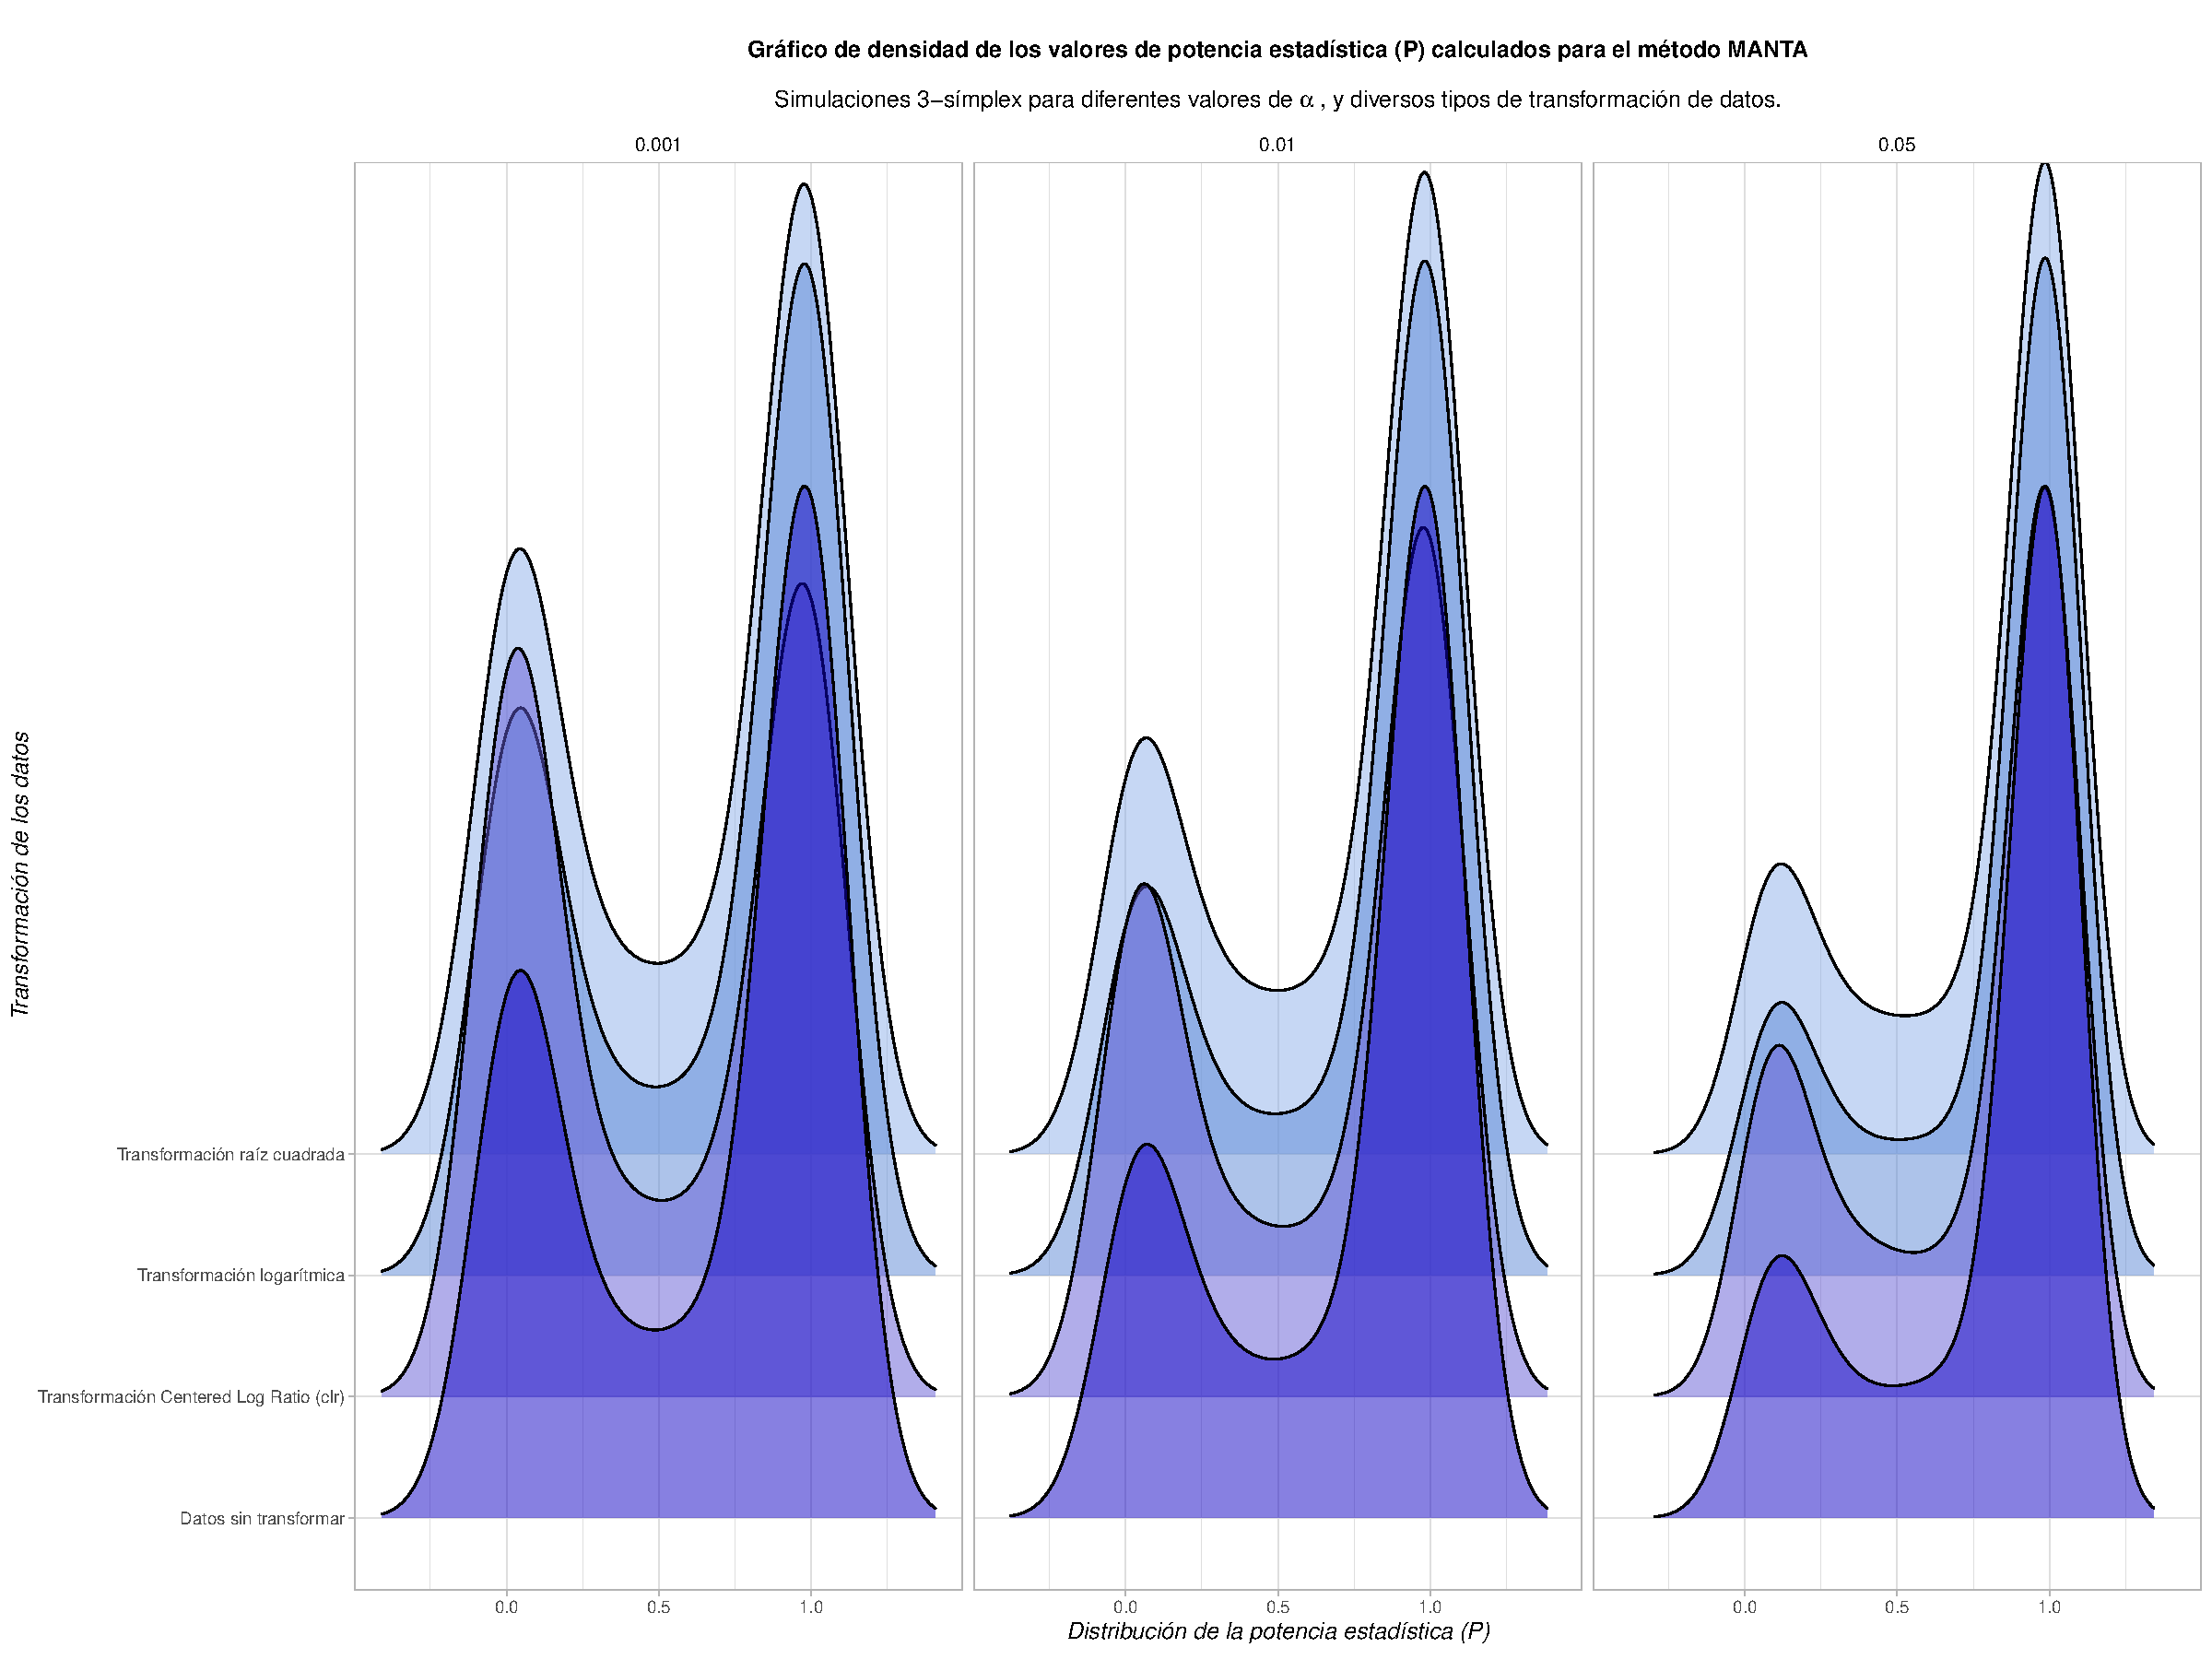
\includegraphics[scale=.3]{OBJ2SimplexStatswrapAlpha.pdf}
    \caption{\scriptsize{A.}}
    \label{figAppend:OBJ2SimplexStatswrapAlpha}
\end{figure}

%OBJ2SimplexStatsGridqloc.pdf
\begin{figure}[!htbp]
\hspace*{-2.1cm} % Movimiento relativo del gráfico
    \centering
    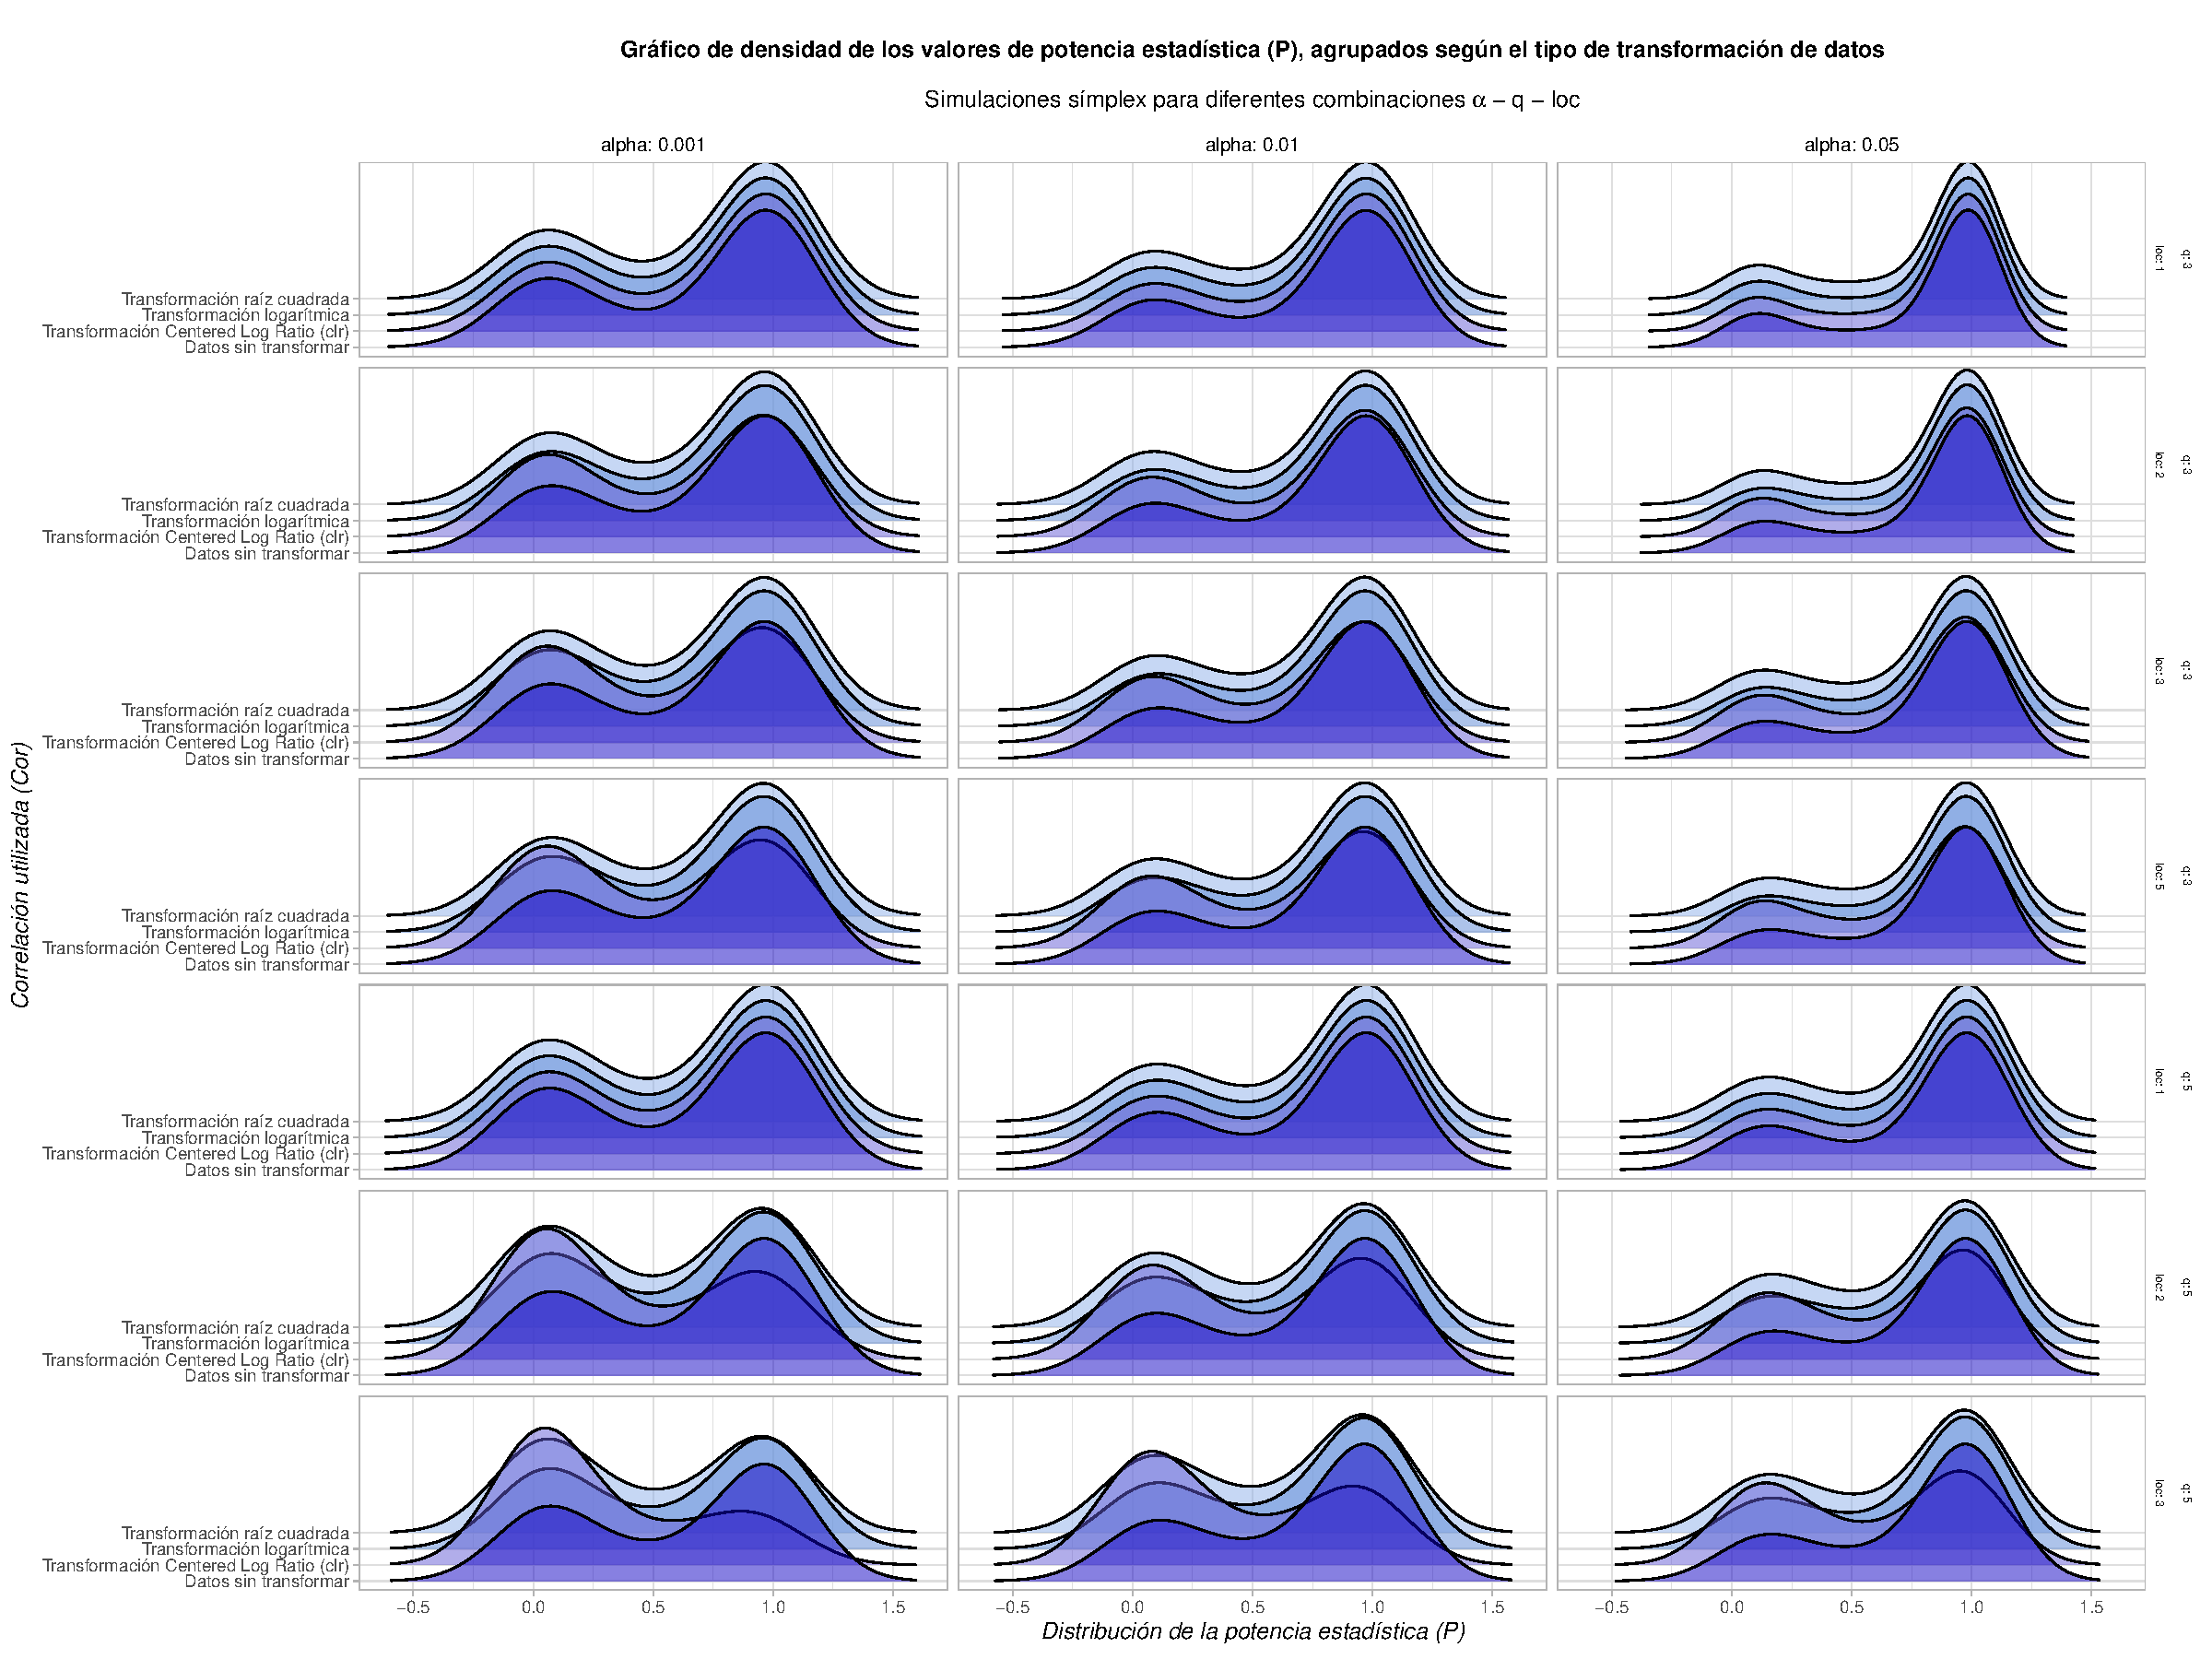
\includegraphics[scale=.3]{OBJ2SimplexStatsGridqloc.pdf}
    \caption{\scriptsize{A.}}
    \label{figAppend:OBJ2SimplexStatsGridqloc}
\end{figure}

% OBJ2SimplexMANTAqloc005.pdf
\begin{figure}[!htbp]
\hspace*{-0.8cm} % Movimiento relativo del gráfico
    \centering
    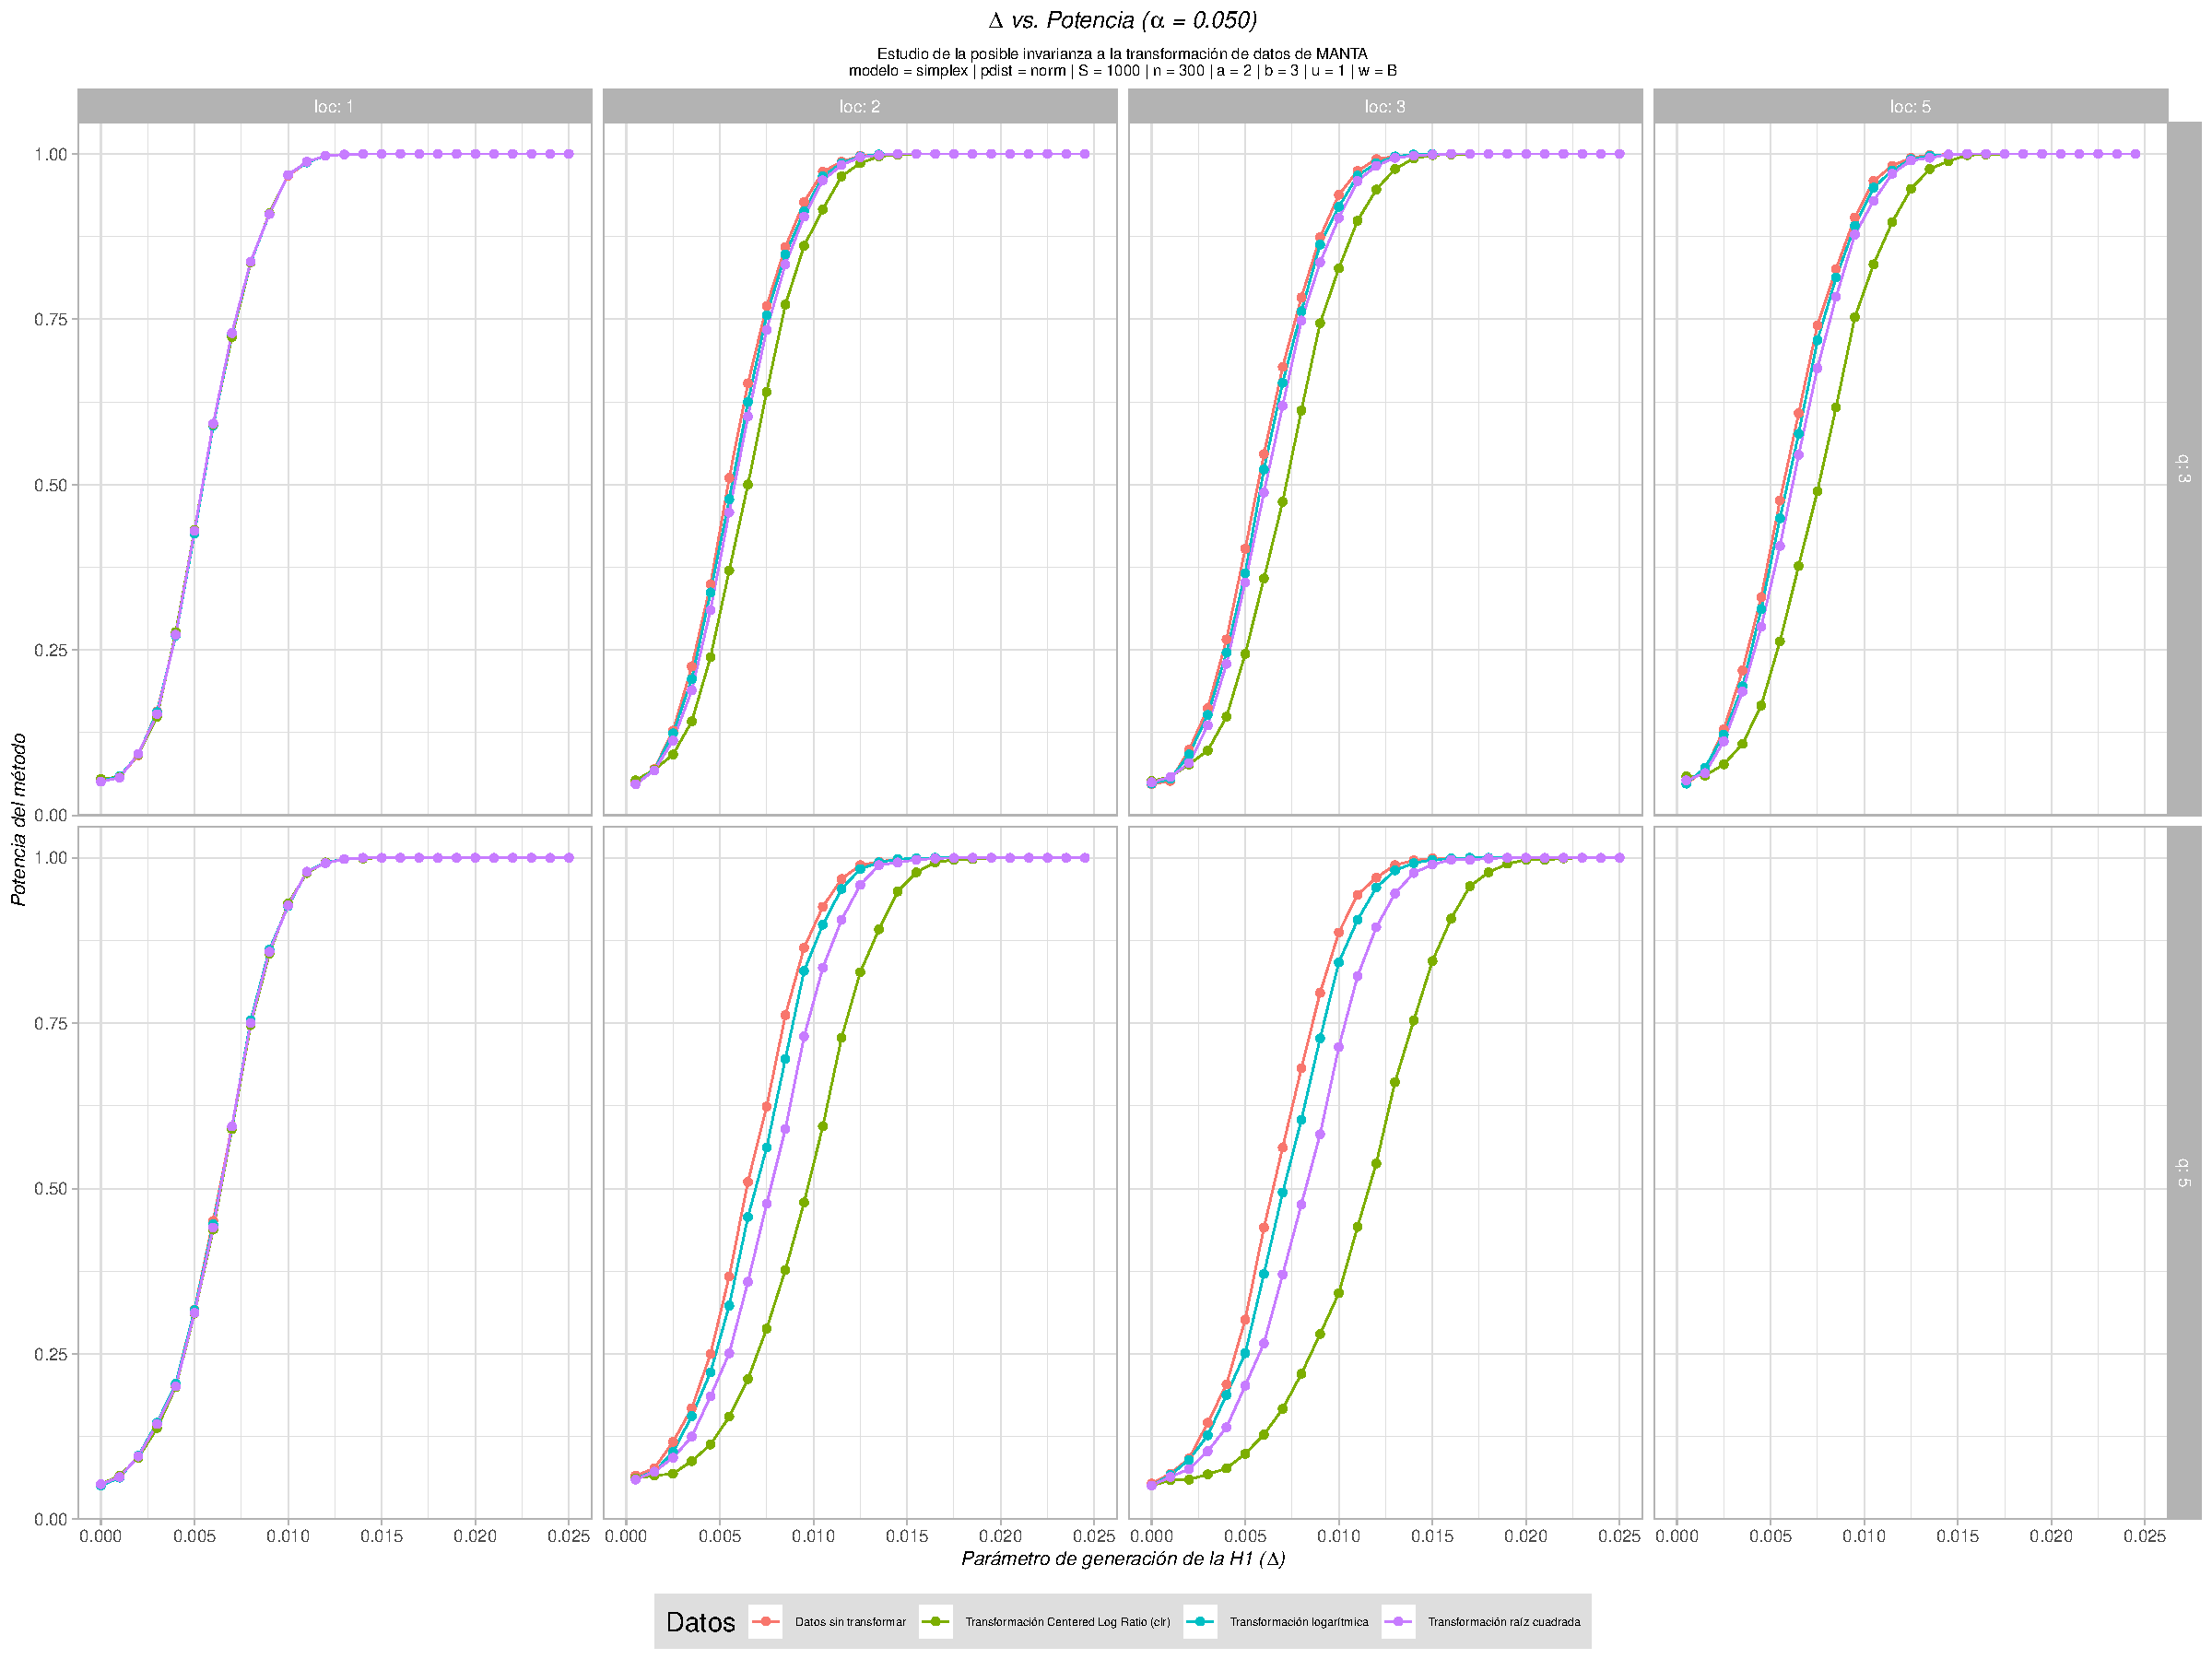
\includegraphics[scale=.45]{OBJ2SimplexMANTAqloc005.pdf}
    \caption{\scriptsize{A.}}
    \label{figAppend:OBJ2SimplexMANTAqloc005}
\end{figure}

% OBJ2SimplexMANTAqloc005ColaIzq.pdf
% OBJ2SimplexMANTAqloc005Coladch.pdf
\begin{figure}[!htbp]
\hspace*{-2cm} % Movimiento relativo del gráfico
\begin{subfigure}{.65\textwidth}
  \centering
  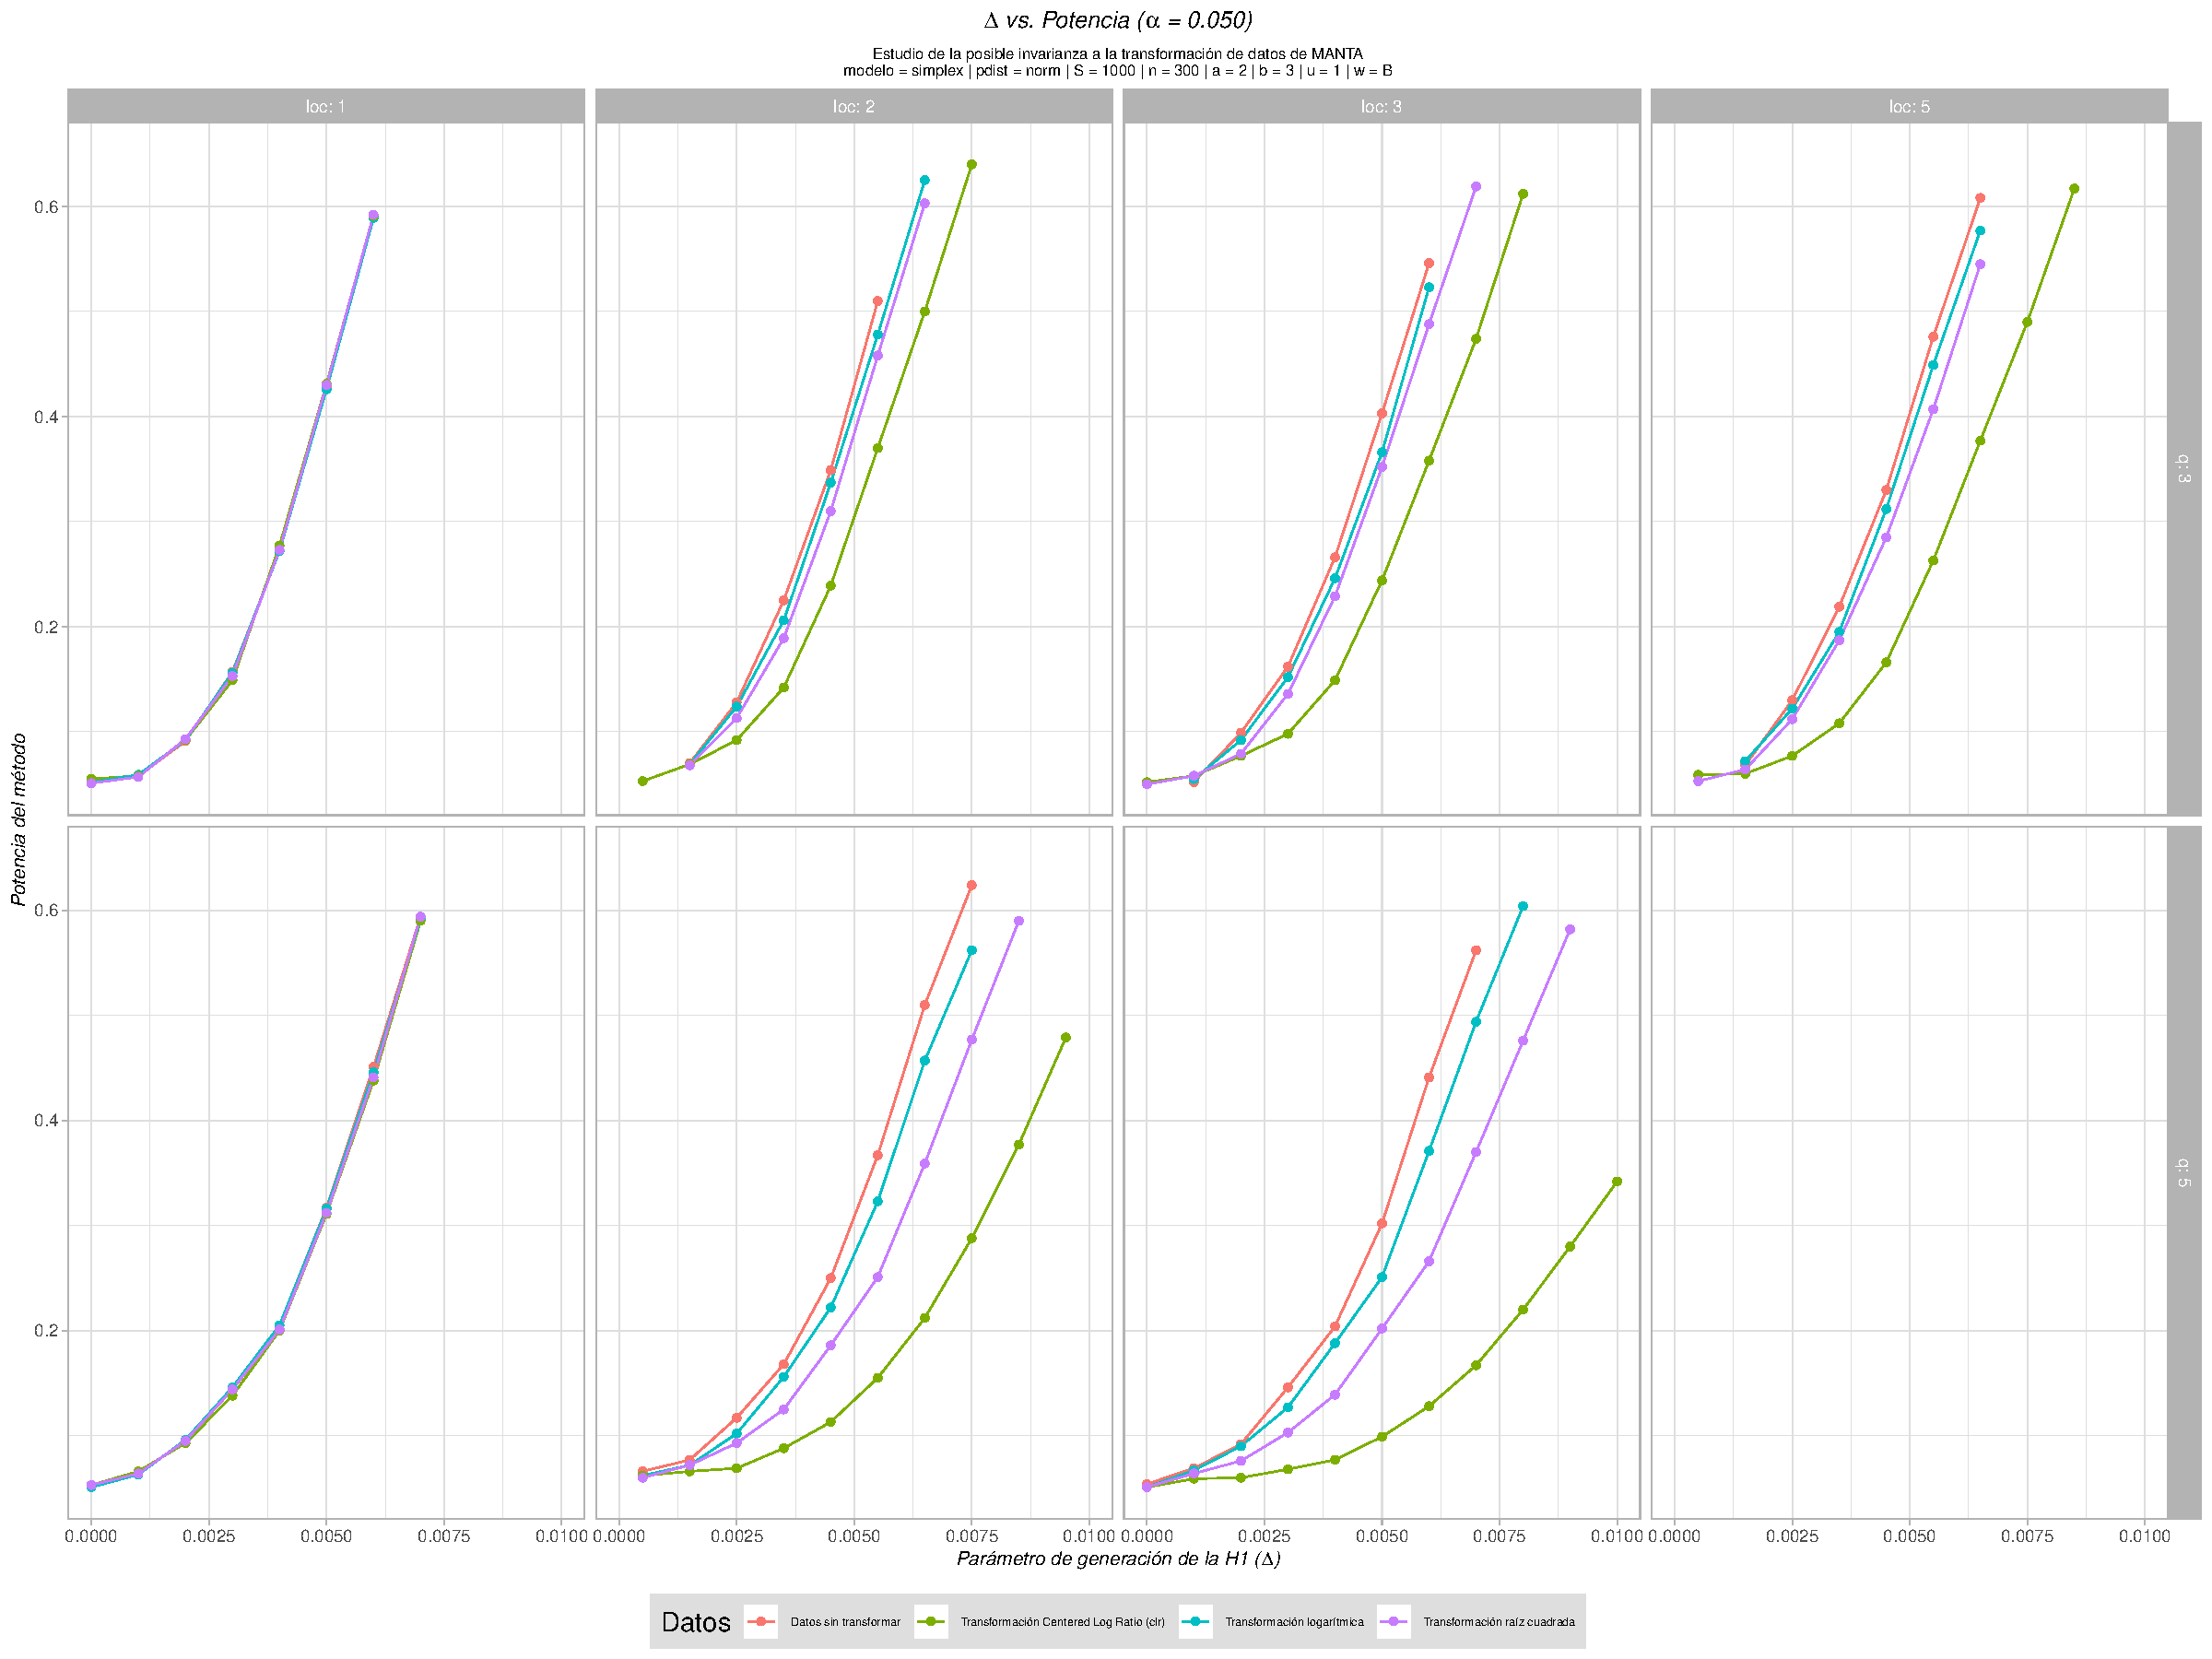
\includegraphics[width=.7\linewidth]{OBJ2SimplexMANTAqloc005ColaIzq.pdf}
  \caption{\scriptsize{A.}}
  \label{figAppend:OBJ2SimplexMANTAqloc005ColaIzq}
\end{subfigure}%
\begin{subfigure}{.65\textwidth}
\hspace*{-2.3cm} % Movimiento relativo del gráfico
  \centering
  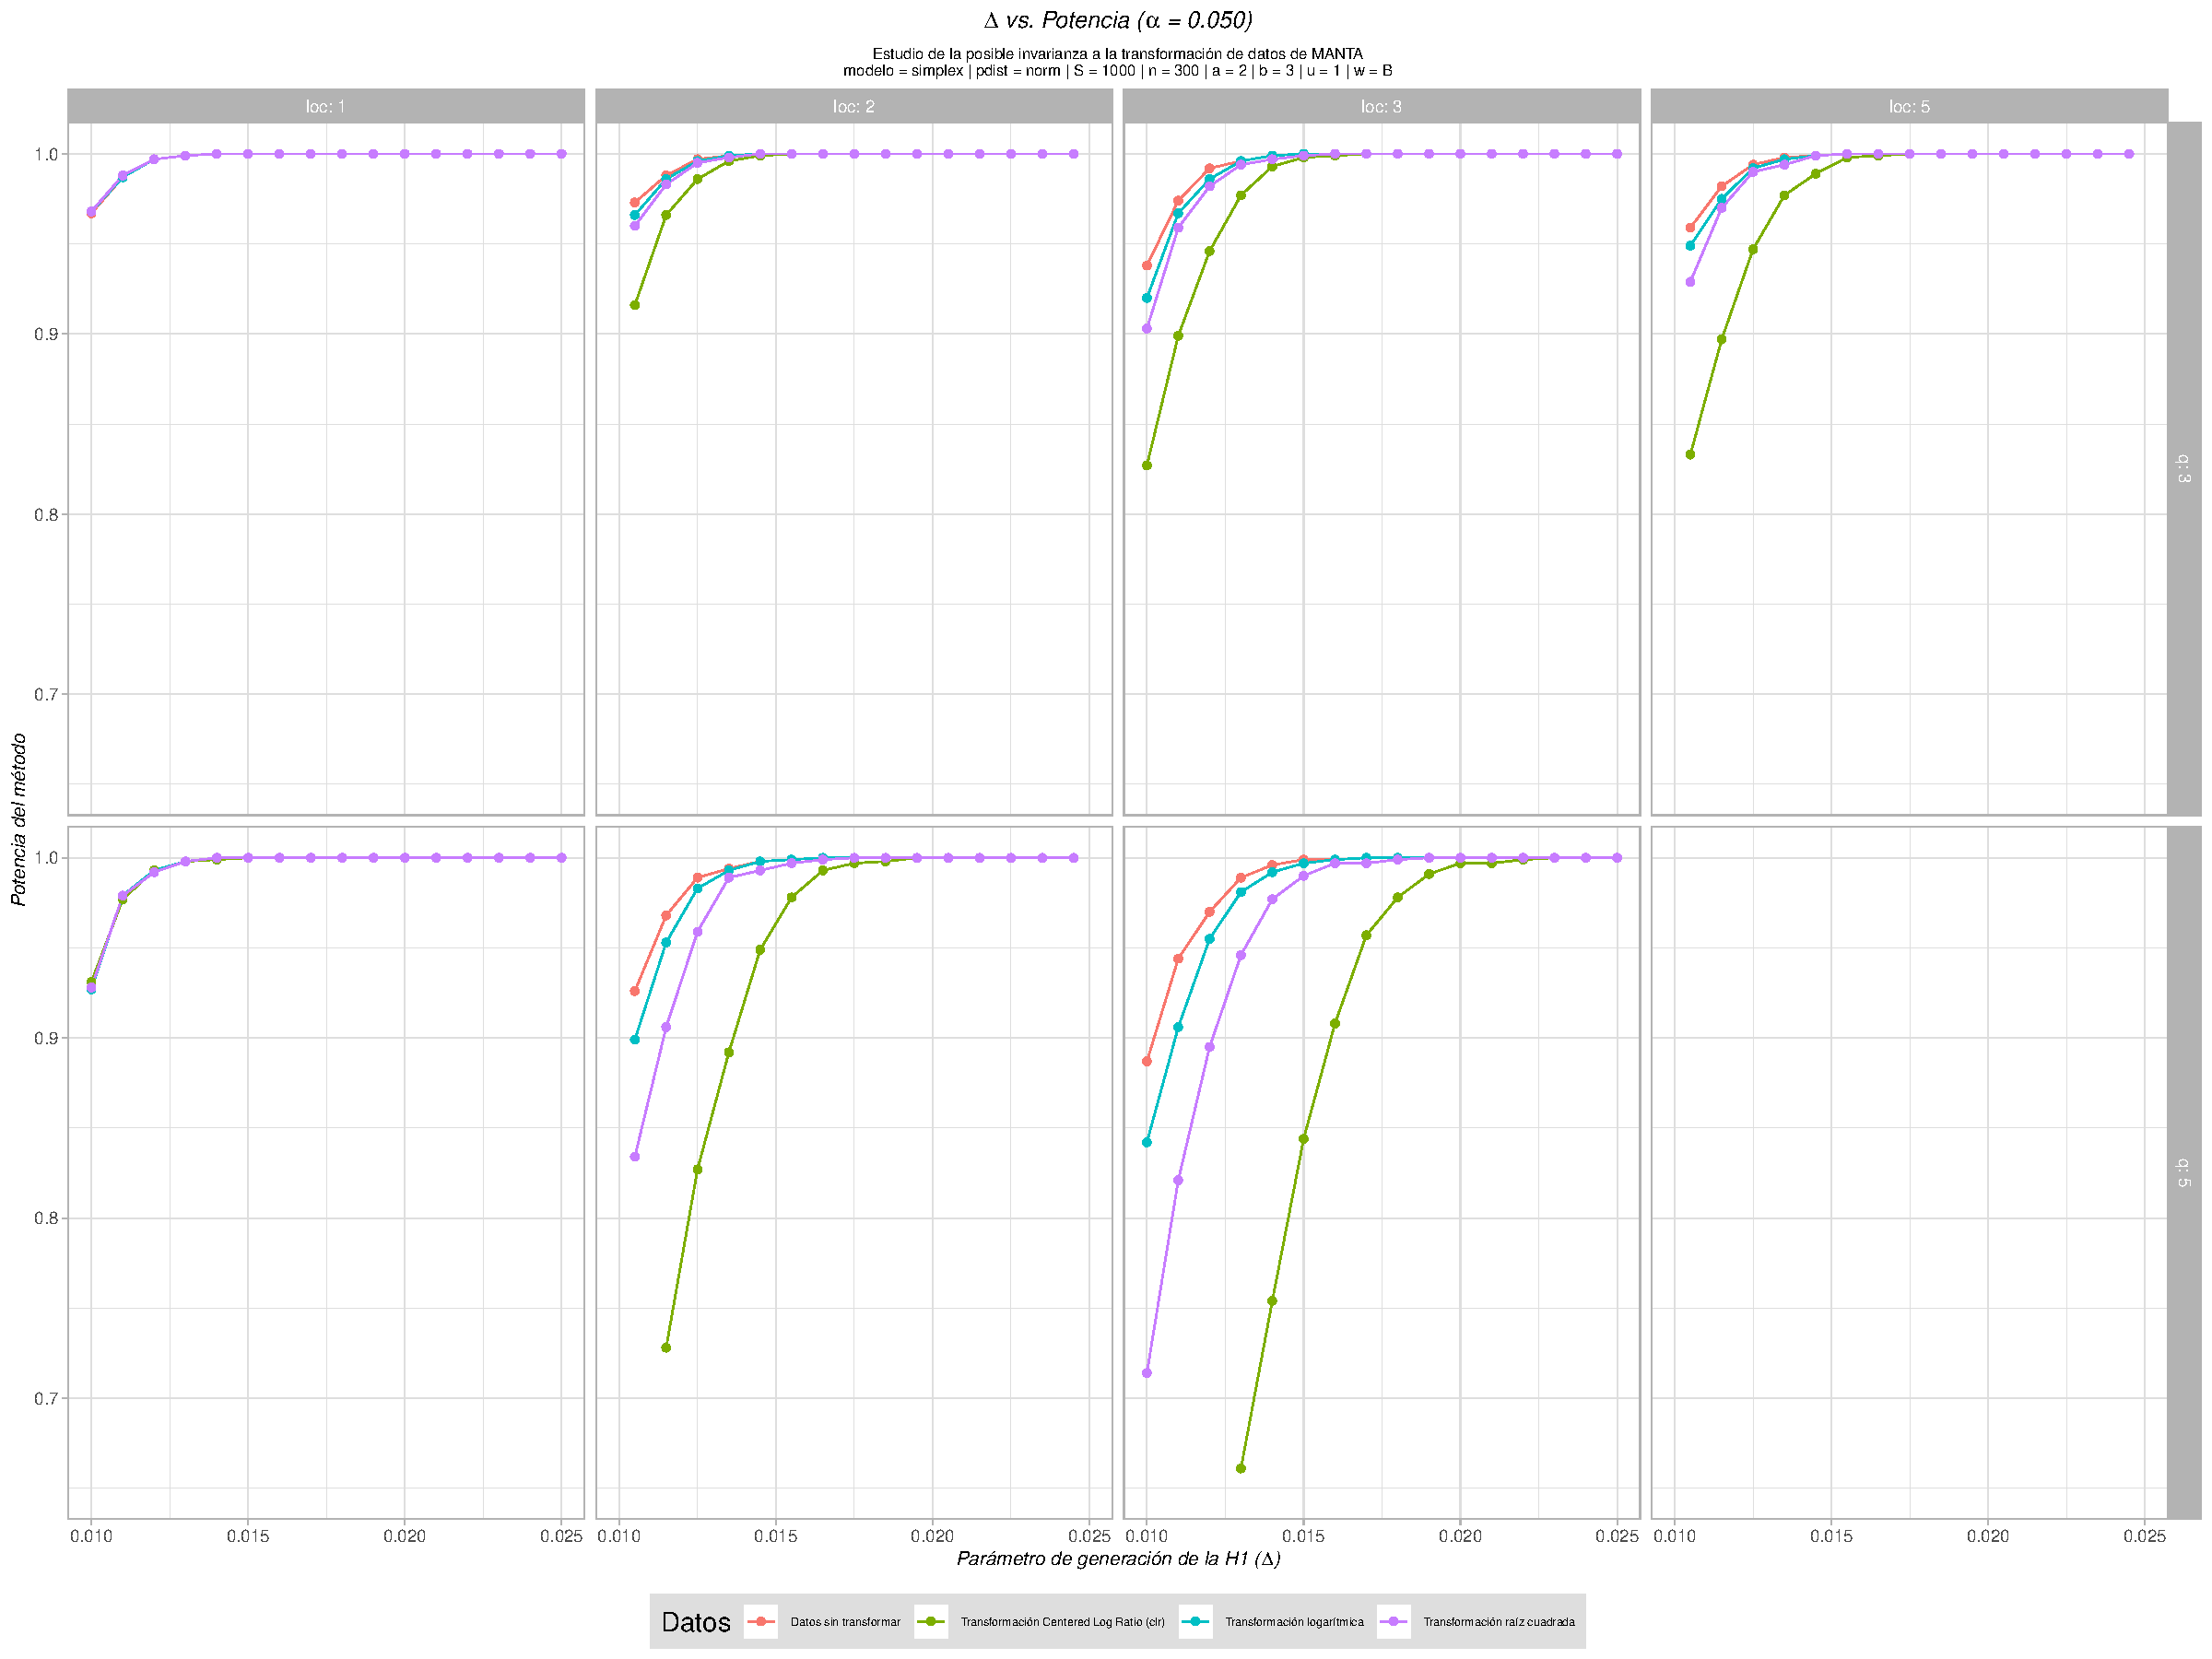
\includegraphics[width=.7\linewidth]{OBJ2SimplexMANTAqloc005Coladch.pdf}
  \caption{\scriptsize{A.}}
  \label{figAppend:OBJ2SimplexMANTAqloc005Coladch}
\end{subfigure}
\caption{\scriptsize{A.}}
\label{figAppend:OBJ2005zoom}
\end{figure}

% OBJ2SimplexMANTAqloc001.pdf
\begin{figure}[!htbp]
\hspace*{-0.8cm} % Movimiento relativo del gráfico
    \centering
    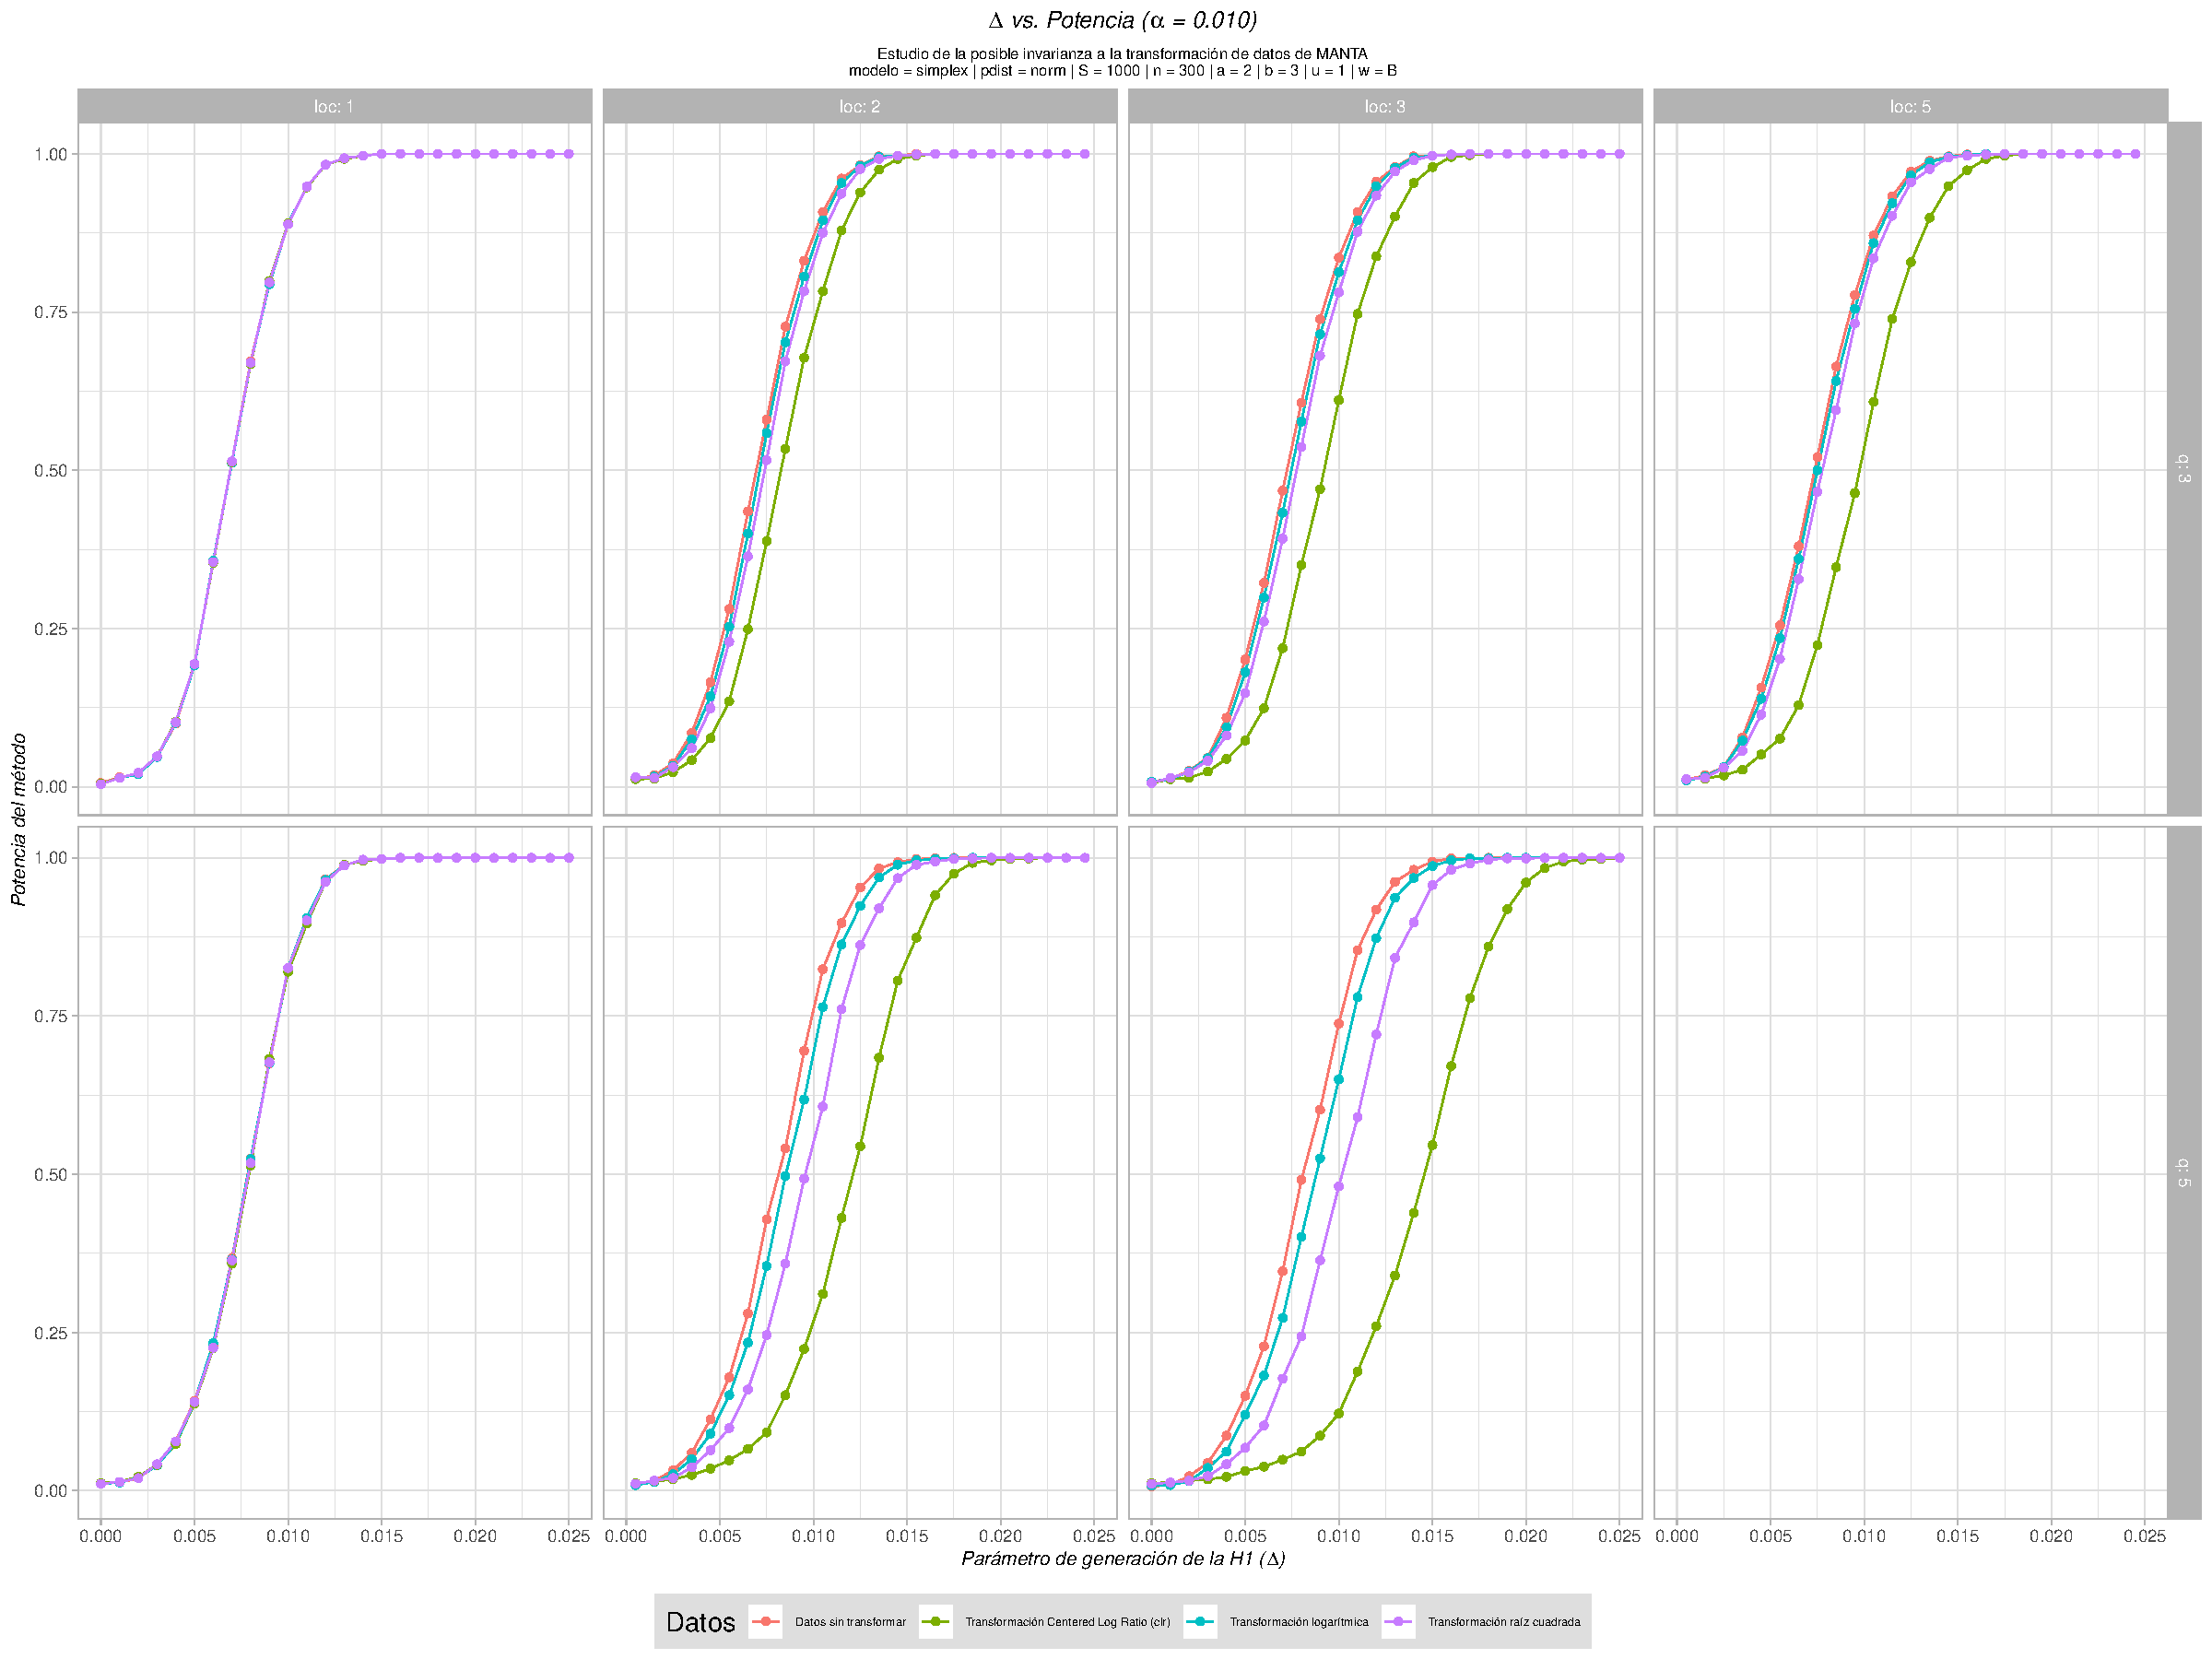
\includegraphics[scale=.45]{OBJ2SimplexMANTAqloc001.pdf}
    \caption{\scriptsize{A.}}
    \label{figAppend:OBJ2SimplexMANTAqloc001}
\end{figure}

% OBJ2SimplexMANTAqloc001ColaIzq.pdf
% OBJ2SimplexMANTAqloc001Coladch.pdf
\begin{figure}[!htbp]
\hspace*{-2cm} % Movimiento relativo del gráfico
\begin{subfigure}{.65\textwidth}
  \centering
  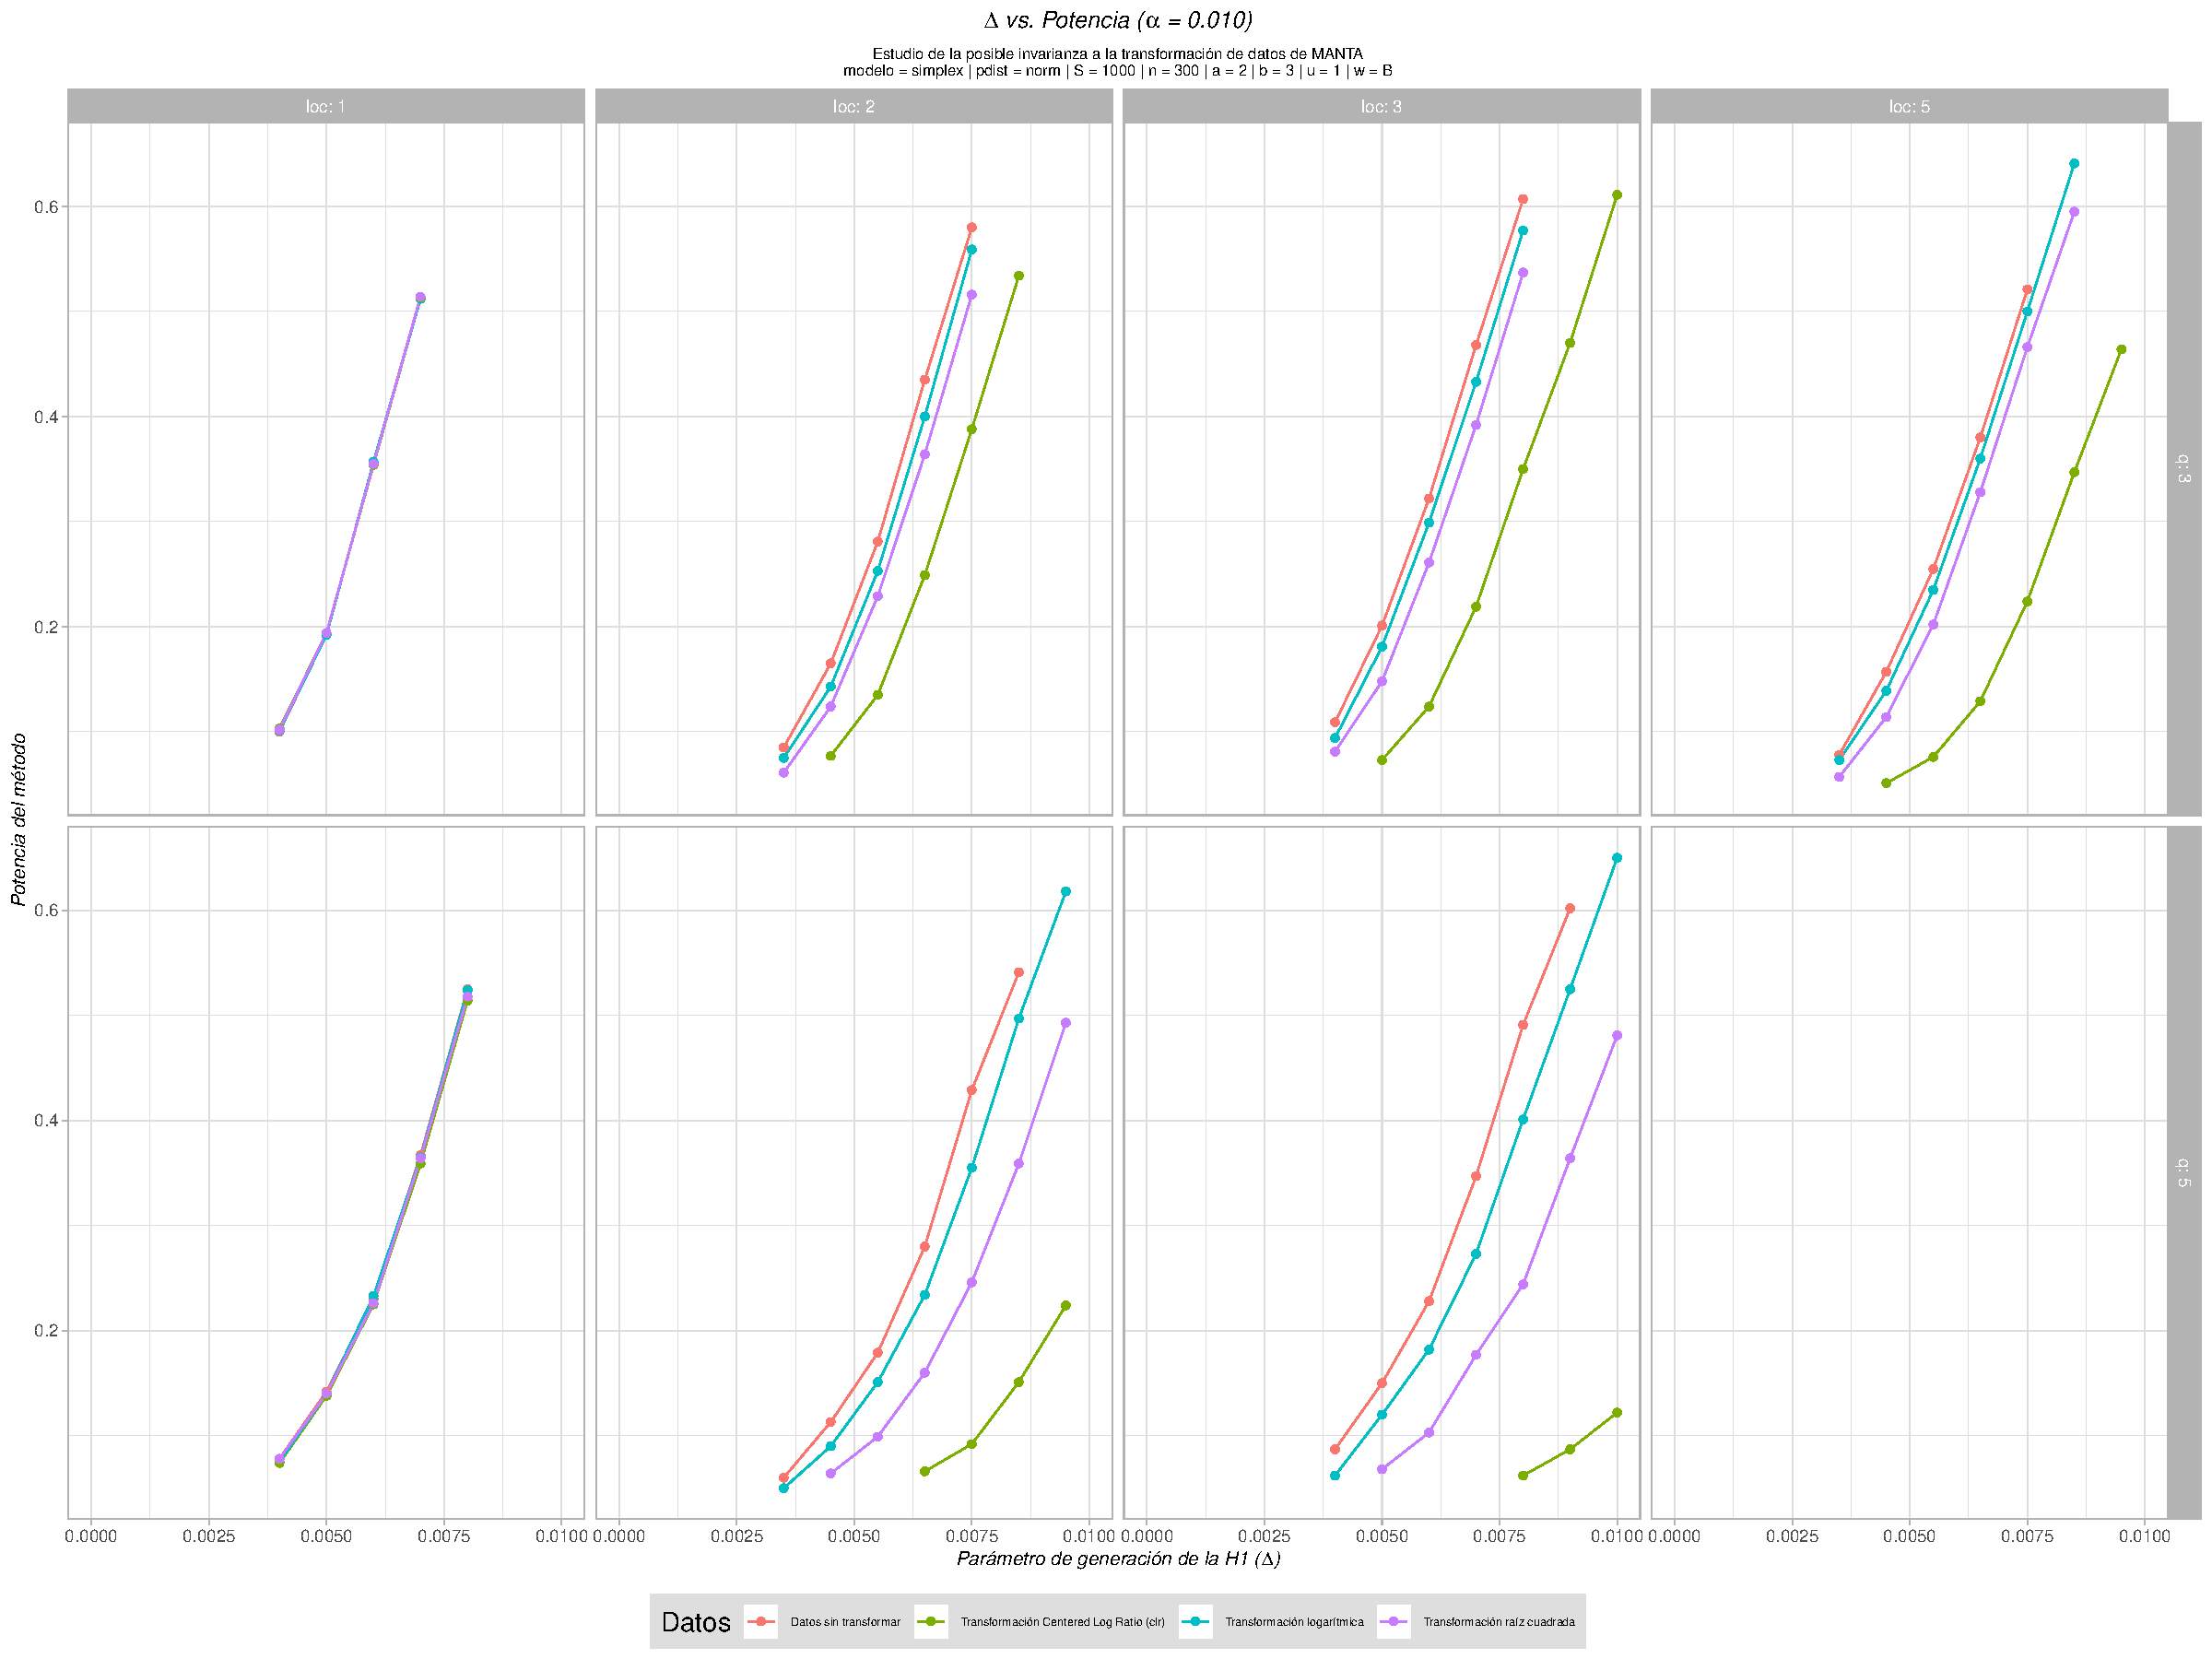
\includegraphics[width=.7\linewidth]{OBJ2SimplexMANTAqloc001ColaIzq.pdf}
  \caption{\scriptsize{A.}}
  \label{figAppend:OBJ2SimplexMANTAqloc001ColaIzq}
\end{subfigure}%
\begin{subfigure}{.65\textwidth}
\hspace*{-2.3cm} % Movimiento relativo del gráfico
  \centering
  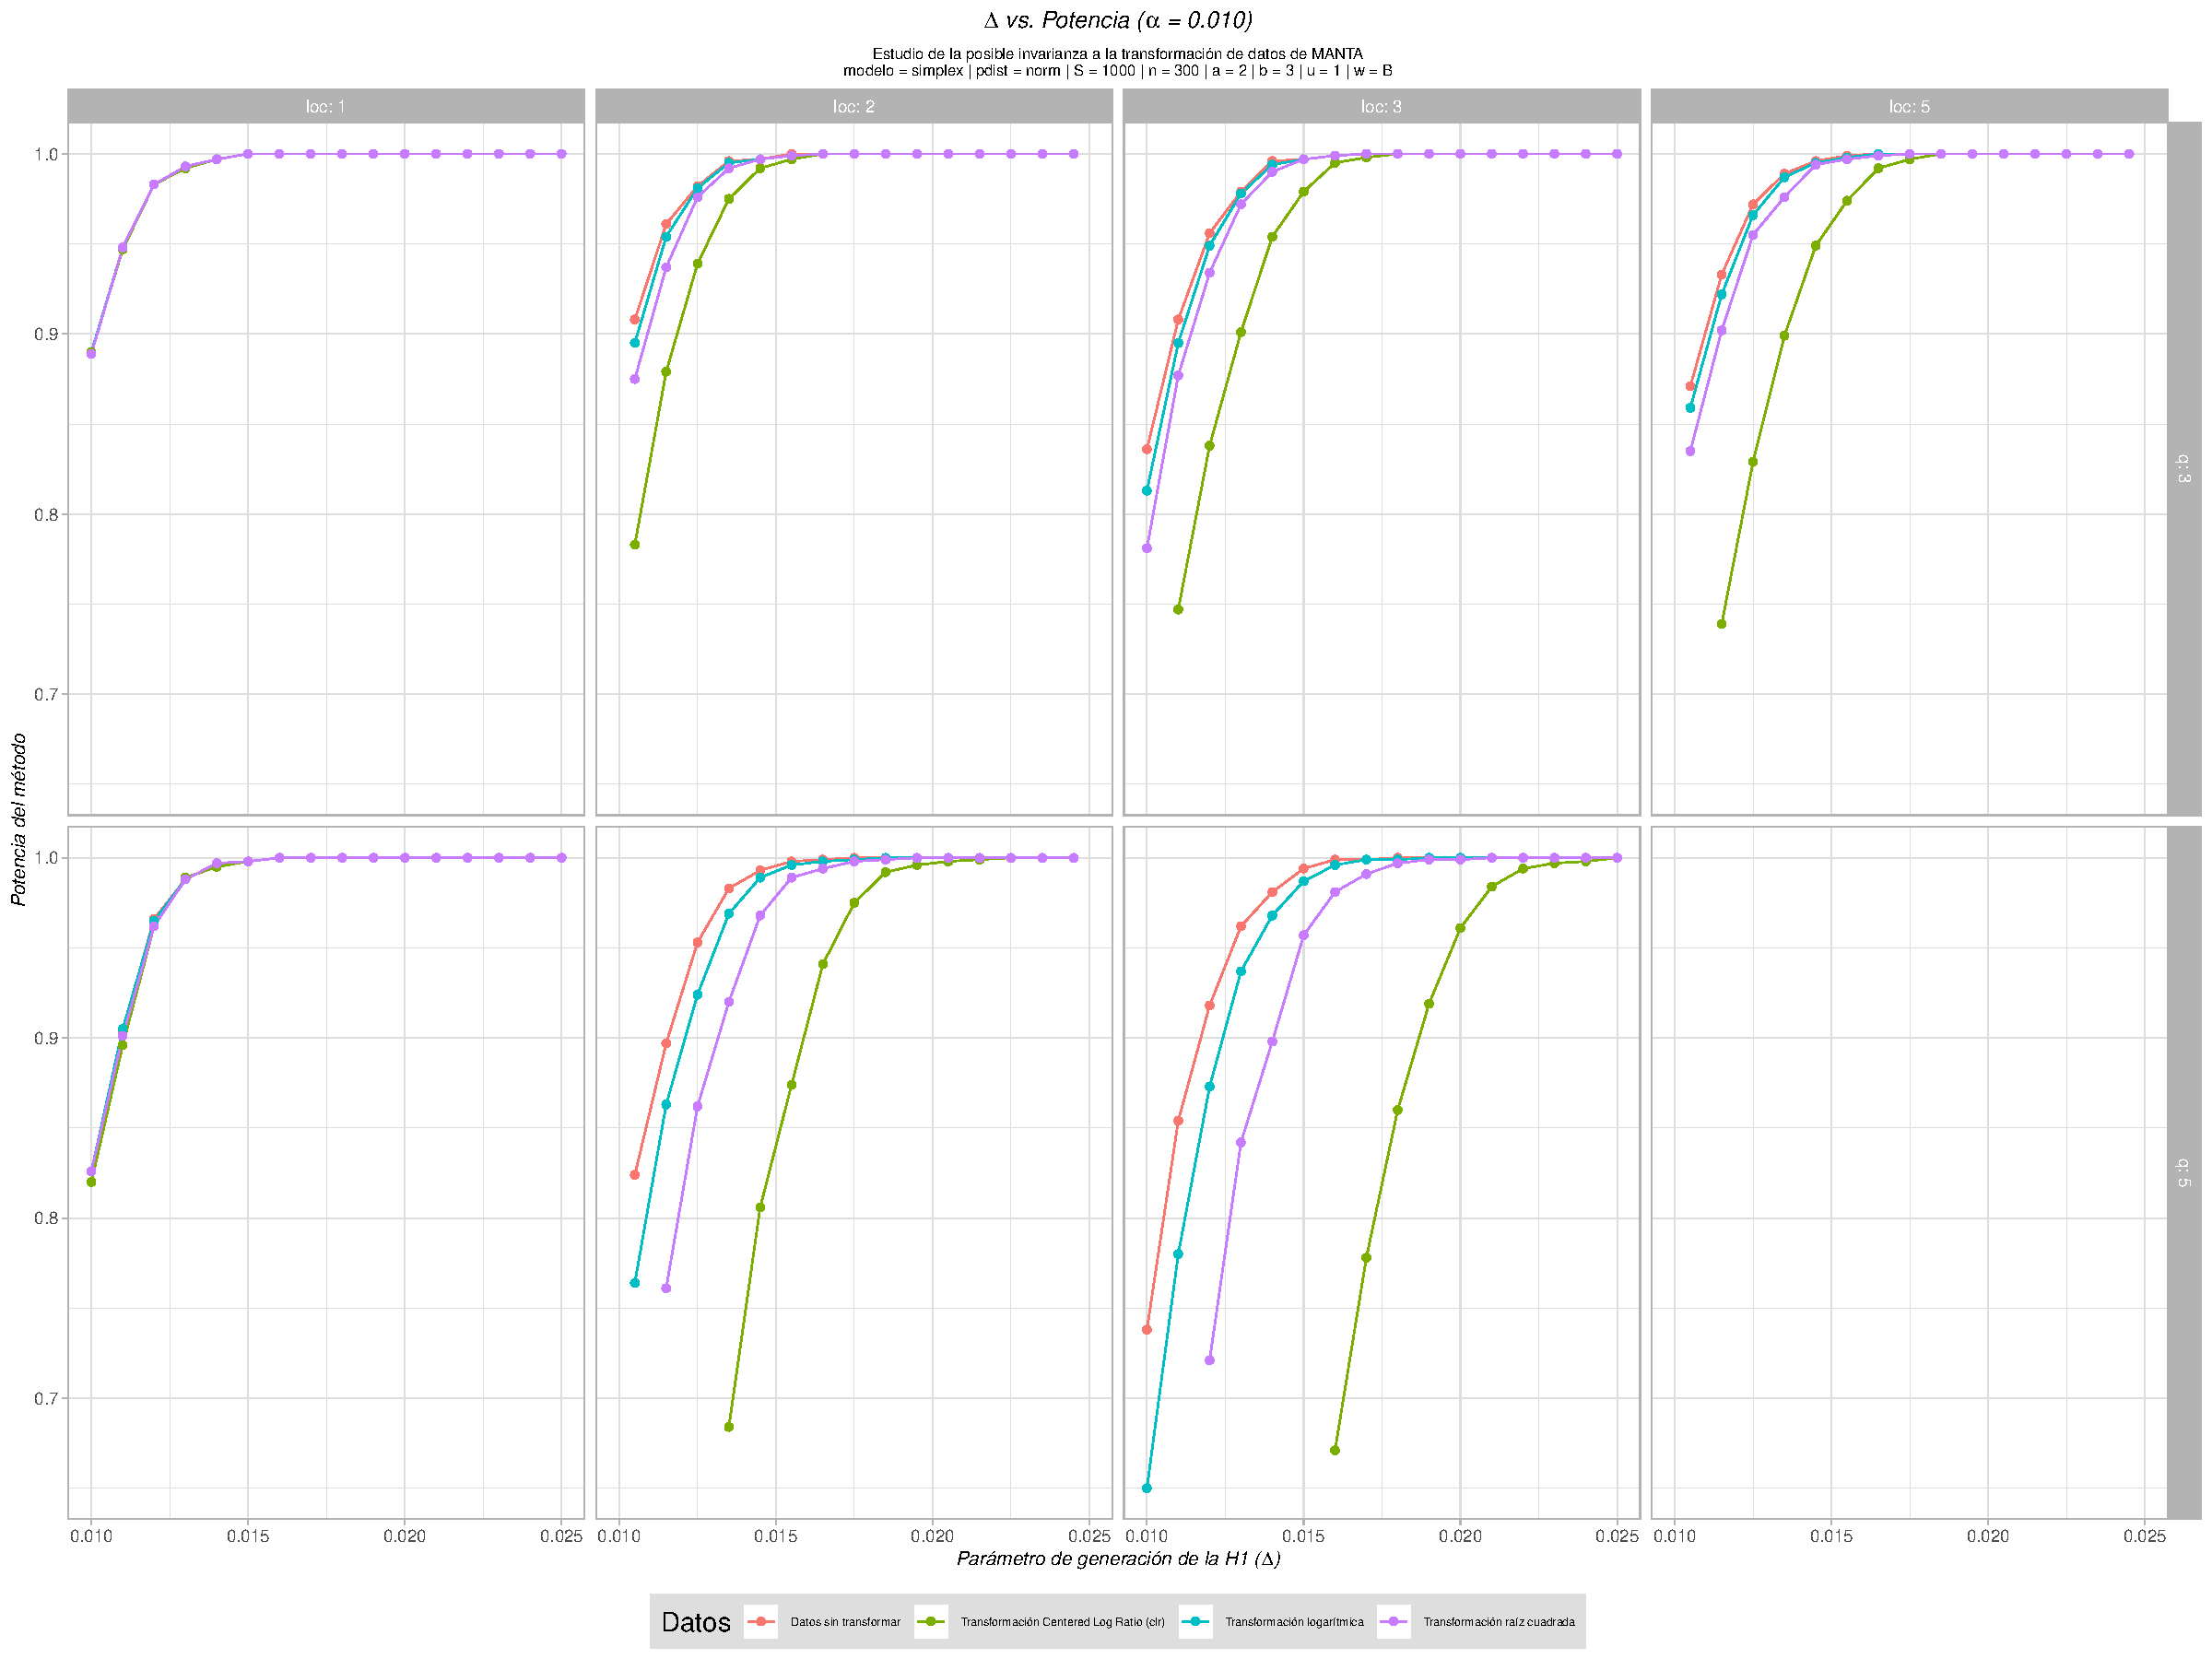
\includegraphics[width=.7\linewidth]{OBJ2SimplexMANTAqloc001Coladch.pdf}
  \caption{\scriptsize{A.}}
  \label{figAppend:OBJ2SimplexMANTAqloc001Coladch}
\end{subfigure}
\caption{\scriptsize{A.}}
\label{figAppend:OBJ2001zoom}
\end{figure}

% OBJ2SimplexMANTAqloc0001.pdf
\begin{figure}[!htbp]
\hspace*{-0.8cm} % Movimiento relativo del gráfico
    \centering
    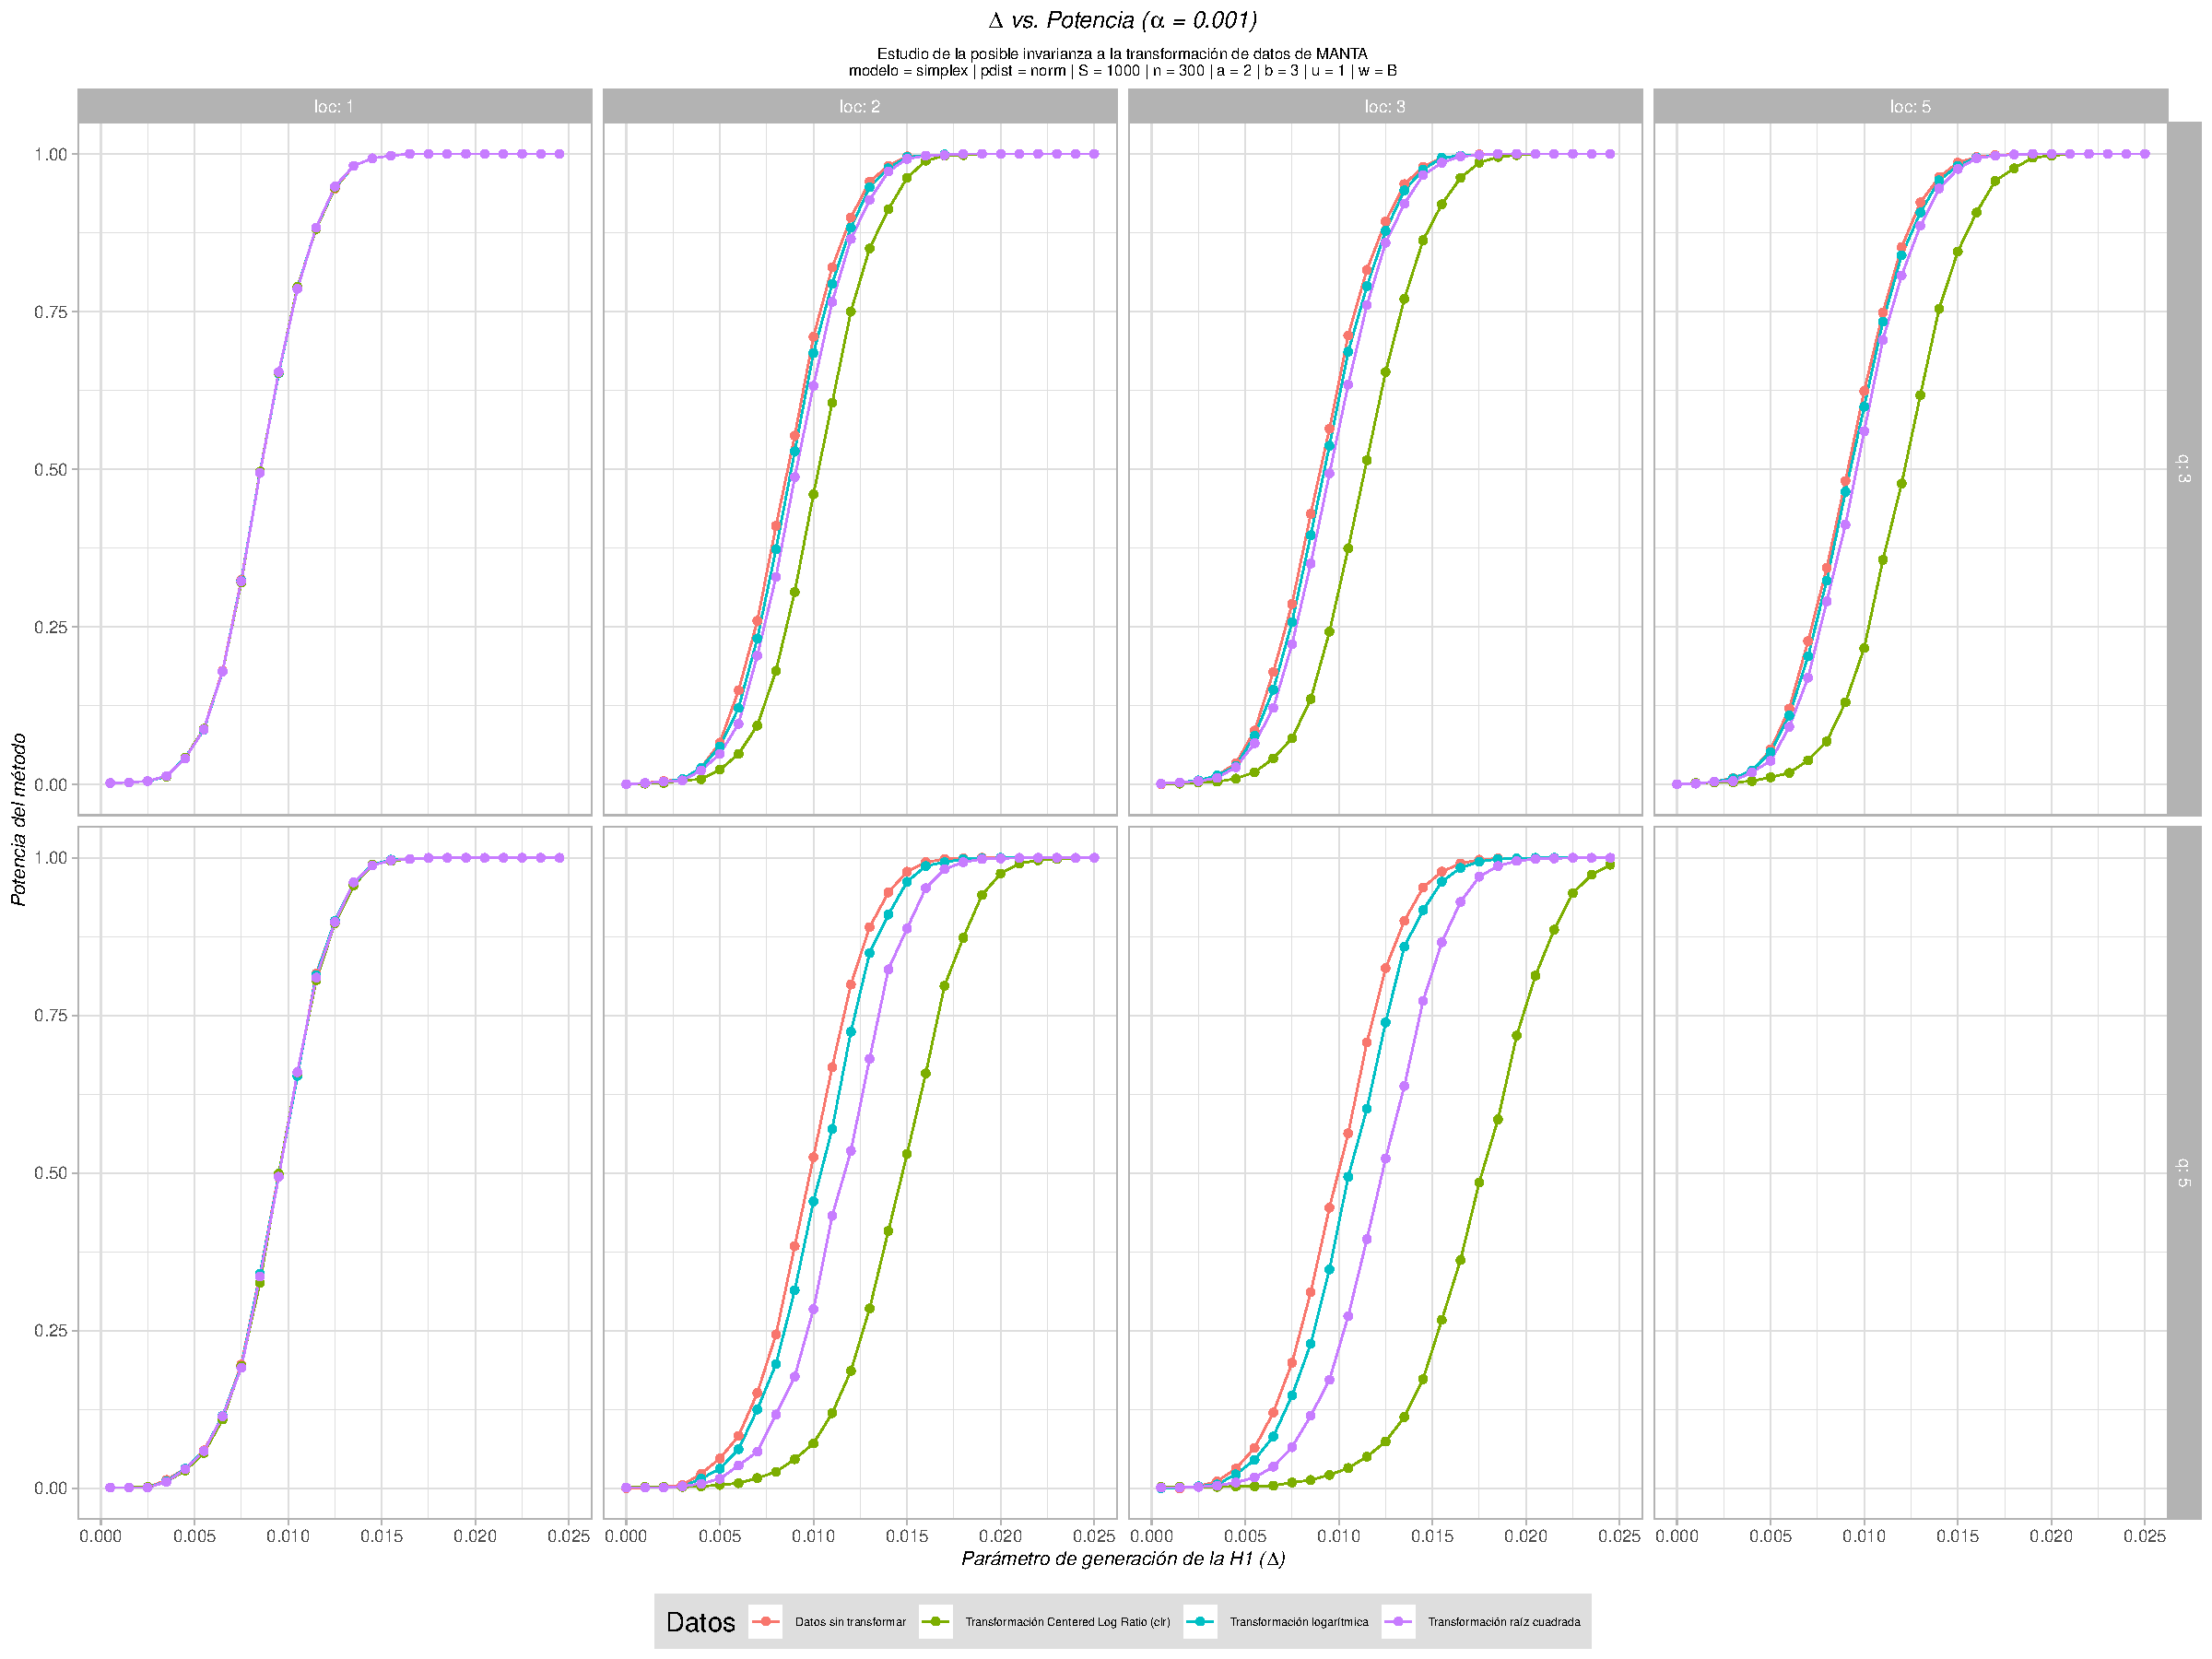
\includegraphics[scale=.45]{OBJ2SimplexMANTAqloc0001.pdf}
    \caption{\scriptsize{A.}}
    \label{figAppend:OBJ2SimplexMANTAqloc0001}
\end{figure}

% OBJ2SimplexMANTAqloc0001ColaIzq.pdf
% OBJ2SimplexMANTAqloc0001Coladch.pdf
\begin{figure}[!htbp]
\hspace*{-2cm} % Movimiento relativo del gráfico
\begin{subfigure}{.65\textwidth}
  \centering
  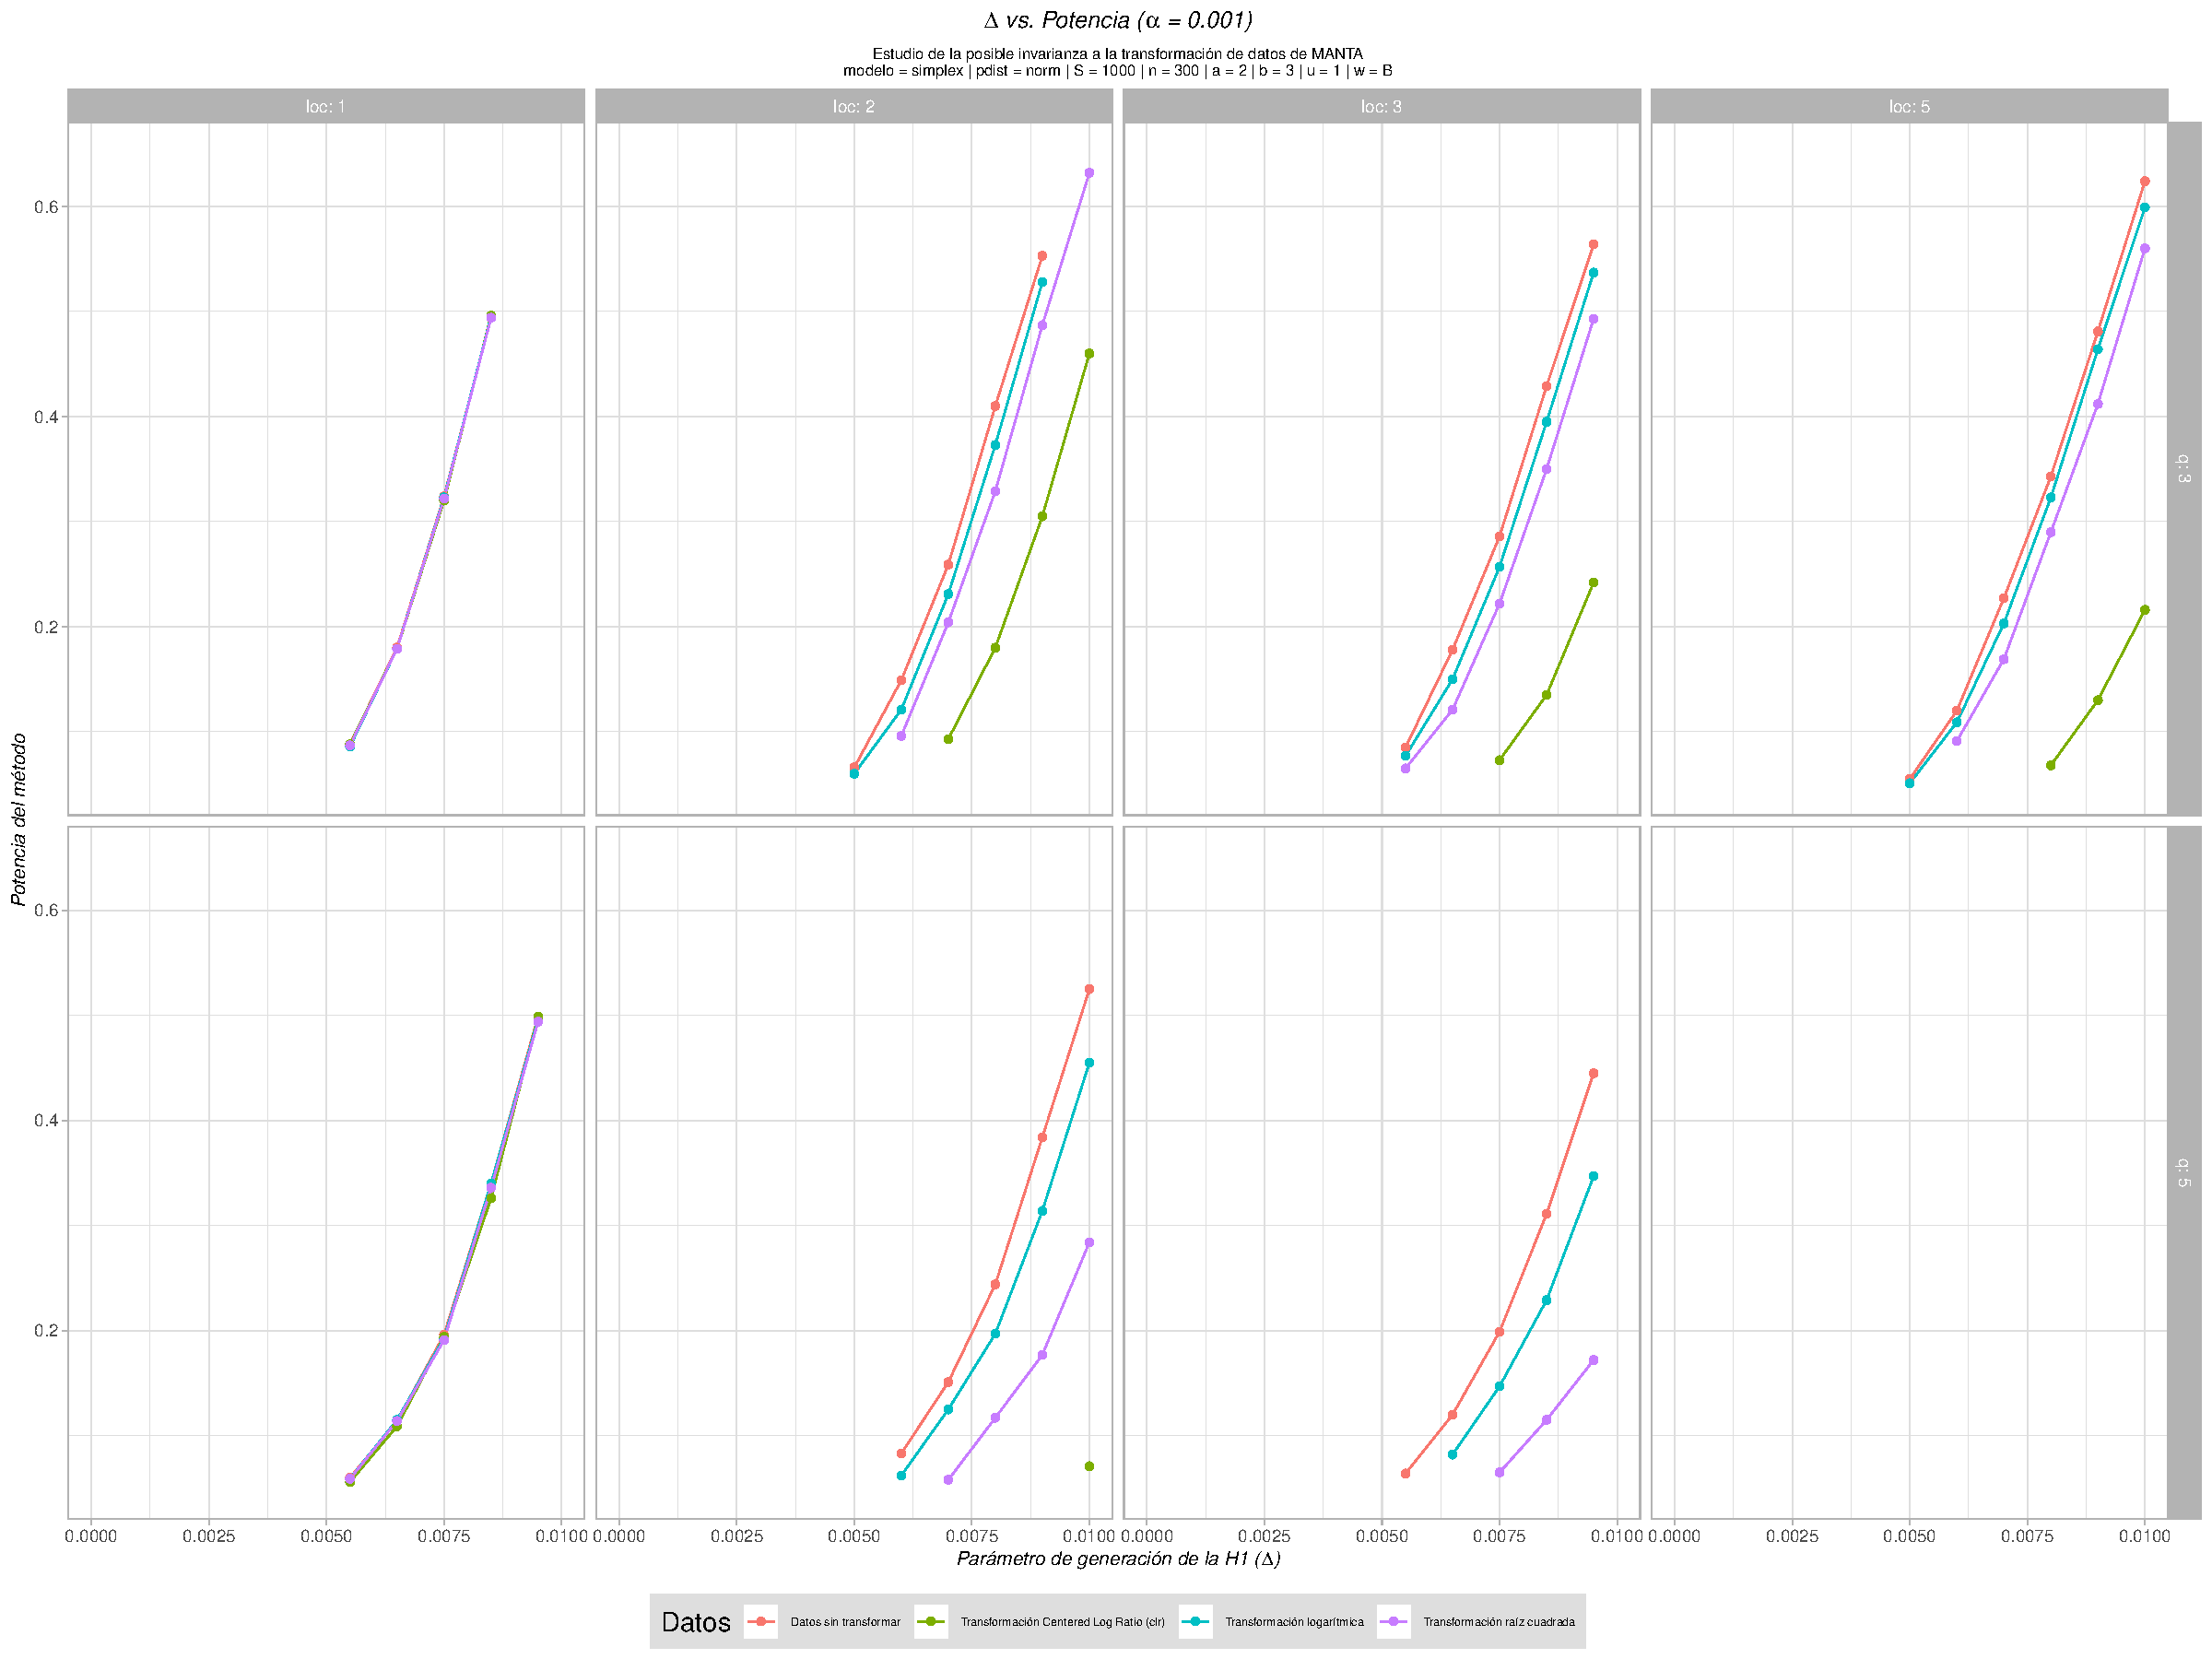
\includegraphics[width=.7\linewidth]{OBJ2SimplexMANTAqloc0001ColaIzq.pdf}
  \caption{\scriptsize{A.}}
  \label{figAppend:OBJ2SimplexMANTAqloc0001ColaIzq}
\end{subfigure}%
\begin{subfigure}{.65\textwidth}
\hspace*{-2.3cm} % Movimiento relativo del gráfico
  \centering
  \includegraphics[width=.7\linewidth]{OBJ2SimplexMANTAqloc0001Coladch.pdf}
  \caption{\scriptsize{A.}}
  \label{figAppend:OBJ2SimplexMANTAqloc0001Coladch}
\end{subfigure}
\caption{\scriptsize{A.}}
\label{figAppend:OBJ20001zoom}
\end{figure}



% -------------------------------------------------------------------------------------------------------%
% -------------------------------------------------------------------------------------------------------%
% ----------------------------------- U  T  I  L  I  D  A  D  E  S --------------------------------------%
% -------------------------------------------------------------------------------------------------------%
% -------------------------------------------------------------------------------------------------------%

% %%%%%%%%%%%%%%%%%%%%%%%%%%%%%%
% % Para introducir ecuaciones %
% %%%%%%%%%%%%%%%%%%%%%%%%%%%%%%
% 
% % Introducir una ecuación numerada y con etiqueta:
% % ------------------------------------------------
% 
% \begin{equation}\label{eq:etiquetaEq}
% Eq
% \end{equation}
% \myequations{Descripción Eq}
% 
% % Referenciar una ecuación:
% % -------------------------
% 
% La ecuación ~\ref{eq:etiquetaEq} es ...
% 
% % Poner paréntesis alrededor de una referencia de ecuación:
% % ---------------------------------------------------------
% 
% La ecuación \eqref{eq:pythagoras} es ...
% 
% % Para introducir ecuaciones no numeradas:
% % ----------------------------------------
% 
% \begin{equation*}
% Eq
% end{equation*}
% \myequations{Descripción Eq}
% 
% % Para introducir ecuaciones con diversas fórmulas:
% % -------------------------------------------------
% 
% \begin{align}
% e^{i\pi} & = \cos(\pi) + i\sin(\pi) \notag \\
%          & = -1 .
% \end{align}
% 
% \begin{equation}
%     1 + 1 = 2
% \end{equation}
% \label{eq:2.1}


% -------------------------------------------------------------------------------------------------------%


\end{document}
